% ------------------------------------------------

% 封面內頁 Inner Cover
%
% 封面: 顯示所有封面內容, 但沒有學校Logo)
%     主要用在印刷版, 如精裝版 或 平裝版
%     (使用cover.tex來產生)
%
% 內頁: 顯示所有封面內容, 但有學校Logo
%     主要用在電子版 + 印刷版
%
% 只要是印刷版, 不論是精裝版或平裝版, 都是 封面 (殼/皮) + 內頁.
% 只有在電子版時, 第一頁就是封面內頁.

\DisplayInnerCover

% ------------------------------------------------

% 口試証明文件
\DisplayOral

% ------------------------------------------------

% 摘要 Abstract
% 請根據你的需求去選用中文或英文版
%
% 學校要求如果是寫中文版的話
% 則要同時交出英文版
%
% 只交英文版就不用交中文版
%
% 詳細學校的要求可去附件看
%
% Place your Chinese abstract here. The abstract heading will be
% generated automatically.
% Note: do NOT use \begin{abstract} ... \end{abstract}
%
\begin{figure}[h]
\centering
\vspace{-29mm}
\begin{tabular}{c}
\hspace{-36mm} 
\includegraphics[]{./abstract/ChineseAbstract1.pdf}
\end{tabular}
\end{figure}
\newpage
\newpage

\begin{figure}[h]
\centering
\vspace{-29mm}
\begin{tabular}{c}
\hspace{-36mm} 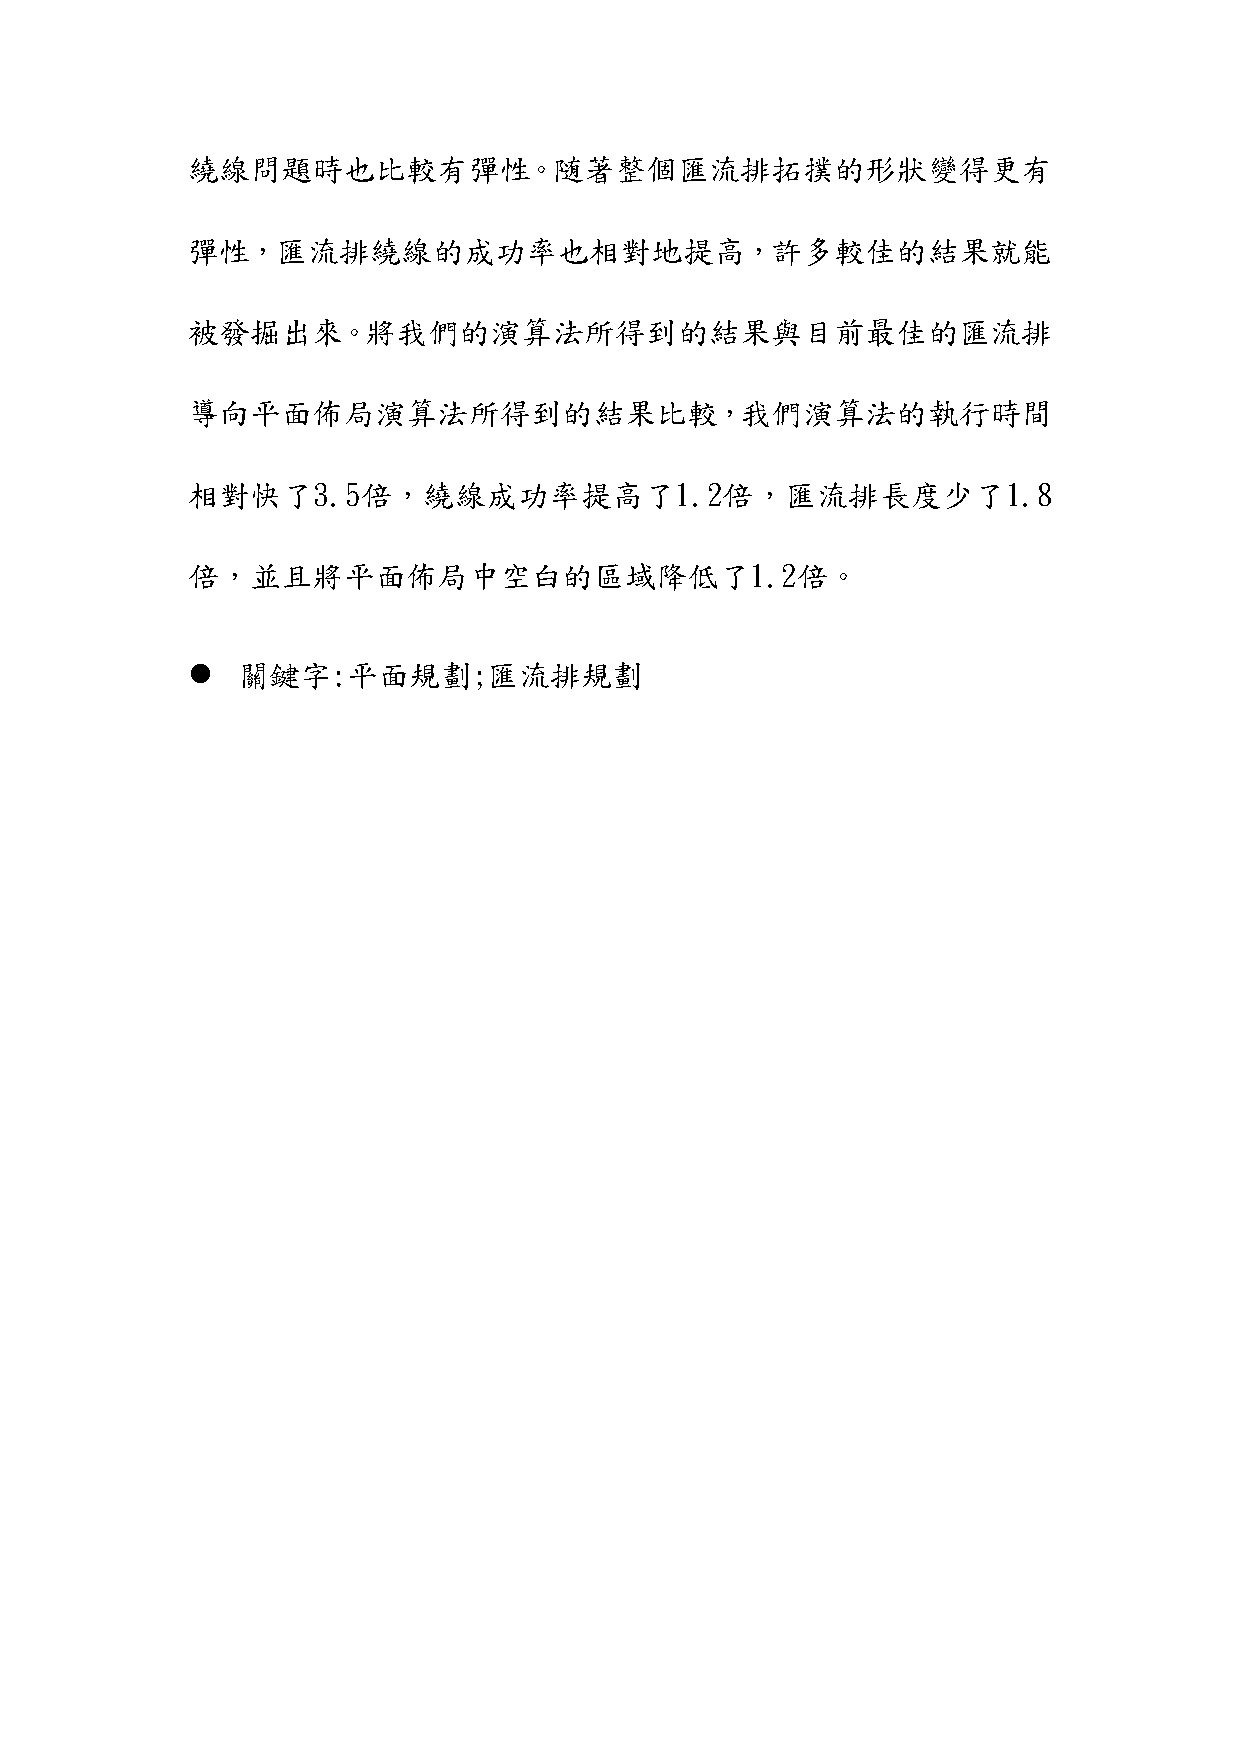
\includegraphics[]{./abstract/ChineseAbstract2.pdf}
\end{tabular}
\end{figure}
\newpage
\newpage



%
% Place your English abstract here. The abstract heading will be
% generated automatically.
% Note: do NOT use \begin{abstract} ... \end{abstract}
%
\begin{center}
\large \textbf{Bus-Pin-Aware Bus-Driven Floorplanning} \\[15mm]
\normalsize \textbf{Student: Po-Hsun Wu \hspace{5mm} Advisor: Dr. Tsung-Yi Ho\\[7mm]}
\normalsize \textbf{Department of Computer Science and\\
                    Information Engineering \\
                    National Cheng Kung University\\
                    Tainan, Taiwan, R.O.C.\\[7mm]}
\large \textbf{Abstract}
\end{center}
%%%%%%%%%%%%%%%%%%%%%%%%%%
\label{abs}
%%%%%%%%%%%%%%%%%%%%%%%%%%

\baselineskip=26pt


As the number of buses increase substantially in multi-core SoC
designs, the bus planning problem has become the dominant factor
in determining the performance and power consumption of SoC
designs. To cope with the bus planning problem, it is desirable to
consider this issue in early floorplanning stage. Recently,
bus-driven floorplanning problem has attracted much attention in
the literature. However, current algorithms adopt an
over-simplified formulation ignoring the position and
orientation of the bus pins, the chip performance may be deteriorated.
In this paper, we propose the bus-driven
floorplanning algorithm that fully considers the impacts of the bus
pins. By fully utilizing the position and orientation of the bus pins,
bus bendings are not restricted to occur at the modules on the bus,
then it has more flexibility during bus routing. With more
flexibility on the bus shape, the size of the solution
space is increased and a better bus-driven floorplanning solution
can be obtained. Compared with the bus-driven
floorplanner \cite{Ma08}, the experimental results show that our
algorithm performs better in runtime by 3.5$\times$, success rate
by 1.2$\times$, wirelength by 1.8$\times$, and reduced the
deadspace by 1.2$\times$.


\begin{itemize}
\item {\bf Keywords:} Floorplanning; Bus planning

\end{itemize}
               % English Abstract


% ------------------------------------------------

% 致謝 Acknowledgments
% ------------------------------------------------

\ifthenelse{\GetLangEnableChi = 1}
{
  % ------------------------------------------------
\StartAcknowledgmentsChi
% ------------------------------------------------

在這邊寫你的感謝 (對父母, 老師, 同學, 朋友等的感謝).

% ------------------------------------------------
\EndAcknowledgments
% ------------------------------------------------

}{}

\ifthenelse{\GetLangEnableEng = 1}
{
  % ------------------------------------------------
\StartAcknowledgments{chapter:acknowledgments}
% ------------------------------------------------

Thanks someone you want here.

Ask Google\cite{website:google} if you need. (If you set some references file, you need to use at least one cite to make Latex work.)

% ------------------------------------------------
\EndAcknowledgments
% ------------------------------------------------

}{}

% ------------------------------------------------


% ------------------------------------------------

% 目錄 (內容, 圖表和圖片) Index of contents, tables and figures.
% 內容會自動產生 The indices will generate in automate.
\DisplayIndex                 % 顯示索引
\DisplayTablesIndex   % 顯示表格索引
\DisplayFiguresIndex  % 顯示圖片索引

% ------------------------------------------------

% Introduction chapter
%% ------------------------------------------------
\StartChapter{Introduction}{chapter:introduction}
% ------------------------------------------------

\StartSection{介紹}

這是國立成功大學碩博士用畢業論文的LaTex模板. 本模板是使用學校最新的畢業論文要求來設計(參考: 附錄 - 撰寫論文須知 P.\RefPage{appendix:thesis-spec}).

雖然本模板的目標是為了提供學生可以使用LaTex來寫畢業論文. 但是各系所有各自的格式, 所以做了一個表列出已知的系所情況(參考: 附錄 - 可使用的系所 P.\RefPage{appendix:acceptable-dept}), 故請在使用前先留意自己的系所有沒有格式要求. 如果沒有, 則本模板應該是可以用來使用; 否則要看系所上的格式, 是否跟本模板有相同的寫法.

本模板分以下幾個主要部份來進行教學:
\begin{enumerate}
  \item 本模板的架構設計
  \item 設定本模板的一些資料以轉成你的論文
  \item 介紹Latex和本模板所提供的語法
  \item 最後有一個chapter為"老師們的話"(Chap. \RefTo{chapter:words-from-teacher})寫了一些老師對論文的想法和意見, 以供同學們留意
\end{enumerate}
同學們只要閱讀完後, 把部份的檔案直接copy和修改內容, 應該很快就能上手本模板去寫自己的論文.

另外在附錄(appendix)附上了一些重要的學校的文件, 由於本模板很接近完善, 故直接使用本模板後可不需再閱過學校相關規定之文件, 所以該類文件置於此僅為備考用.

% ------------------------------------------------
%\newpage

\begin{description}
  \item[版權 License] \hfill
  \InsertImage
    [scale=0.8, align=center,
      caption={CC Attribution-NonCommercial-ShareAlike License},
      label={fig:appendix:by-nc}]
    {./example/introduction/pic/by-nc-sa.png}

    本著作(ncku-thesis-templete-latex\RefBib{web:this-project:github})採用創用 CC 姓名標示-非商業性-相同方式分享 4.0 授權條款.

    This work(ncku-thesis-templete-latex\RefBib{web:this-project:github}) is licensed under Creative Commons Attribution-NonCommercial-ShareAlike 4.0 International License.

  詳細請看'LICENSE'這檔案中的條款說明.

  \item[版本修改 ChangeLog] \hfill
    % ------------------------------------------------
\begin{description}
  \item[v1.3.0] 重大改版 (如果是使用升級方式, 請注意以下所修改的部份有沒有影響自身的版本)\hfill
    \begin{description}
      \item[其他] \hfill
        \begin{enumerate}
          \item 更新CONTRIBUTE中的名單和使用的稱號
        \end{enumerate}
    \end{description}

  \item[v1.2.8] 修正日期在英文書脊中, 會因月份文字的長度而影響位置不一樣的問題

  \item[v1.2.7] \hfill
    \begin{enumerate}
      \item 增加可放置論文題目的長度. 修正在封面和Oral文件的樣板中, 會在題目沒有很長情況下, 被強迫斷行. 長度控制交由同學自己斷行, 以造出比較漂亮題目
      \item 修正書脊中題目跟學位不是同一個高度的問題
      \item 修正英文Oral文件的樣板會出現頁碼的問題
    \end{enumerate}

  \item[v1.2.5] 修正在'Objective'和'Acknowledgments'的錯誤內容

  \item[v1.2.4] 增加英文封面可同時顯示中英文 (\href{https://github.com/wengan-li/ncku-thesis-templete-latex/issues/3}{Issue \#3})

  \item[v1.2.3] \hfill
    \begin{enumerate}
      \item 修正統一使用'Fig'去取代'Fig.', 因為當使用'Fig.'時會產生更大的空格
      \item 修正在'表格 Table'中的圖片位置
      \item 移除在'圖片 Image'的'多張'中舊API的說明文字
      \item 修正在'圖片 Image'中插入多張的圖片時, 不管是主圖或子圖片都推薦使用'align = center'來進行置中, 除非是為了特殊的原因
    \end{enumerate}

  \item[v1.2.2] 修正在'Induection'中的'ChangeLog'和'License'中一些奇怪多餘的空白

  \item[v1.2.1] 修正中文書脊文字位置錯誤問題

  \item[v1.2.0] \hfill
    \begin{enumerate}
      \item Appendix新增'常見問題Q\&A'
      \item 把'Induection'中的'ChangeLog'改使用為單一'.tex'檔去存放
      \item 增加字眼'共同指導'或'Co-advisor'在封面上 (\href{https://github.com/wengan-li/ncku-thesis-templete-latex/issues/2}{Issue \#2})
      \item 重新調整中文封面中的中英文名字2邊的中間空間的大小, 以防止中文名字有4個字時, 出現overlap的問題
    \end{enumerate}

  \item[v1.1.6] 刪除'Induection'和'README.md'中的'版本 Version'

  \item[v1.1.5] 修正每個Chapter的第一頁的頁碼位置跟其他頁面不同的問題 (\href{https://github.com/wengan-li/ncku-thesis-templete-latex/issues/1}{Issue \#1})

  \item[v1.1.4] 修正目錄自己沒有在目錄的Linking中出現

  \item[v1.1.3] 修正README.md中內容的位置錯誤

  \item[v1.1.2] \hfill
    \begin{enumerate}
      \item 重寫有關figure API的code, 增加和優化那些功能 (如增加align)
      \item 更新README.md的內容
      \item 增加ChangeLog
    \end{enumerate}

  \item[v1.1.1] \hfill
    \begin{enumerate}
      \item 把'Abstract'的中文版本是以'摘要'來顯示
      \item 修改和改良有關oral文件的一些path位置
    \end{enumerate}

  \item[v1.1.0] \hfill
    \begin{enumerate}
      \item 增加版權資料到一些核心檔案
      \item 修改和增加一些圖書館要求的內容
      \item 修改有關abstract的一些path位置
      \item 正式得到學校有關部門對這模板的接受
    \end{enumerate}

  \item[v1.0.1] 修改少量錯誤的內容和URL連接

  \item[<= v1.0.0] 正式完成版本
\end{description}

% ------------------------------------------------

\end{description}

% ------------------------------------------------
\EndChapter
% ------------------------------------------------


% Objective chapter
%% ------------------------------------------------
\StartChapter{Objective}{chapter:objective}
% ------------------------------------------------

\StartSection{起因}

做這個模版的原因其實很簡單:

\begin{enumerate}
  \item
  {
    去投國外paper時, 對方可能會要求使用LaTeX, 所以未來要懂LaTeX是不意外的.
  } % End of \item{}

  \item
  {
    想拿LaTeX來寫畢業論文, 卻發現學校只提供Mircosoft Word模版, 但卻沒有提供LaTeX的, 所以證明本模版對學校是有存在價值的.
  } % End of \item{}

  \item
  {
    因為看到發現台灣科技大學\RefBib{web:latex:template:ntust}, 台灣大學\RefBib{web:latex:template:ntu}, 元智大學\RefBib{web:latex:yzu}都能找到LaTeX的模版, 連大陸那邊都有一些學校有在提供, 更不用說國外的學校.

    那些學校的畢業論文模版不只提供是Mircosoft Word版本(.doc), 是會連Latex(.tex)版本都有, 而我們學校卻沒有. 唯一我們學校在Google上找到的有提到的卻是數學系系網頁上的功能\RefBib{web:latex:ncku_math_introduction}和建在數學系上的一個討論區\RefBib{web:latex:ncku_math_forum}.
  } % End of \item{}

  \item
  {
    因為學校對Phd跟Master的畢業論文要求是同一個格式, 所以如果完成後對學校任何學生應該都有其好處.

    對大家都有多一個選擇來寫畢業論文, 而不是被限在使用Mircosoft Word來寫.
  } % End of \item{}

  \item
  {
    經過詢問我們資訊工程系(CSIE)的系上一些老師後, 意外發現原來某些實驗室其實已經有各自的版本存在, 但每個版本都有各自的優缺點, 例如:

    \begin{enumerate}

      \item
      {
        新的使用者或接手的人不容易修改或使用.
      } % End of \item{}

      \item
      {
        或是需要安裝的步驟十分麻煩 (e.g cwTeX\RefBib{web:latex:cwtex}).
      } % End of \item{}

      \item
      {
        另外有一些因為是只針對英文版本, 沒有考量在編寫或初稿時會有中英混雜的時候(同時因學校奇怪的要求, 例如英文內容的論文卻要寫中文論文名字等), 所以需要把整個論文分開成不同格式的檔案.
      } % End of \item{}
    \end{enumerate}
  } % End of \item{}
\end{enumerate}

% ------------------------------------------------

\StartSection{目標}
所以為了解決以上的問題, 這個模版針對了好幾點來處理:

\begin{enumerate}

  \item
  {
    把本模版做到連笨蛋都可以很快懂得使用(所謂的Books for Dummies), 所以只留下使用者要填寫的部份外, 其他都交由模版去負責.
  } % End of \item{}

  \item
  {
    希望做到使用者只讀這份模版, 就會懂得去修改和寫自己所需的內容(所謂的Self-contained. 但其實是不太可能的, 因為Latex的使用手冊就算寫成一本幾百頁的書, 都可以缺少很多東西), 所以會同時提供很基本使用Latex的方式, 和填寫本模版步驟.
  } % End of \item{}

  \item
  {
    希望一份模版, 能同時應用在中文或是英文版本, 只要修改內容和一些的設定.
  } % End of \item{}

  \item
  {
    把本模版open source, 讓以後任何的同學們都可以使用和修改, 以合適當時的需求.
  } % End of \item{}

\end{enumerate}

而選擇使用XeLaTex的原因, 是經過分析cwTeX, CJK和XeLaTex後. 發現cwTeX的寫法太糟, 要背多新一種語法, 而且安裝複雜\RefBib{web:latex:cwtex}; 而CJK有一定程度的設定才能在整個論文中自由使用, 感覺設定麻煩而不太能笨蛋化來用, 所以放棄選用; 故最後選用最簡單加一些包裝, 就可以簡單使用中英混合的XeLaTex.

% ------------------------------------------------

\StartSection{缺點}
但是同樣任何東西都會有缺點, 故本模版都不意外:

\begin{enumerate}

  \item
  {
    本模版是以台灣國立成功大學所最新訂下的畢業論文要求(參考: 附錄 - 撰寫論文須知 P.\RefPage{appendix:thesis-spec})來設計, 所以不一定能對非本校的人有用.
  } % End of \item{}

  \item
  {
    對沒有程式基礎, 只會用Mircosoft Word的人來講, 可能會在修改或使用上會十分吃力.
  } % End of \item{}

  \item
  {
    因為我針對某些使用者不用去接觸的部份, 進行了大量的包裝(Wrapping), 所以如果懂得Latex的人可能會覺得我破壞了Latex的語法. 但是本模版是針對笨蛋化和全自動, 我相信對不會的人來講, 才不管這問題 (如同一般理論派和應用派的差別, 在意的方向完全不一樣).
  } % End of \item{}

  \item
  {
    某些包裝出來的語法, 可能會在一些情況下會產生衝突而令Latex不接受, 這時候有2種做法:
    \begin{enumerate}
      \item
      {
        不使用某些寫法, 例如已知的\begin{verbatim}\InsertFigure\end{verbatim}沒法被包在Table, minipage或framebox中.
      } % End of \item{}

      \item
      {
        如真的要使用那些情況, 那只好自己真的不使用我的語法, 而直接去寫Latex原版的語法.
      } % End of \item{}
    \end{enumerate}
  } % End of \item{}
\end{enumerate}

% ------------------------------------------------

\StartSection{總結}

以上是個人對這份模版的一些想法和起源, 同時希望本模版能對你提供到一些幫助.

% ------------------------------------------------
\EndChapter
% ------------------------------------------------


% Related Work chapter
%% ------------------------------------------------
\StartChapter{Related Work}{chapter:related-work}
% ------------------------------------------------

% ------------------------------------------------
\EndChapter
% ------------------------------------------------


% Algorithm chapter
%% ------------------------------------------------
% Page start
% ------------------------------------------------
\chapter{Algorithm}
\label{chapter:algorithm}

\baselineskip=26pt
\thispagestyle{empty}
% ------------------------------------------------

\subsection{Design}

\subsubsection{Li's Hash}

Li's Hash is an algorithm that combines the concept of n-gram indexing \cite{web:wiki:n-gram} (Figure \ref{fig:algorithm:n-gram}), JSON (JavaScript Object Notation) \cite{web:wiki:json} (Figure \ref{fig:algorithm:json_example}) and hash table \cite{web:wiki:hash-table}.\\

JSON to store data which is exactly as same as hash table, but only different of the value's data type, which is because of the mapping design. And the n-gram indexing normally only target the data in string.\\

\begin{figure}[h]
\centering
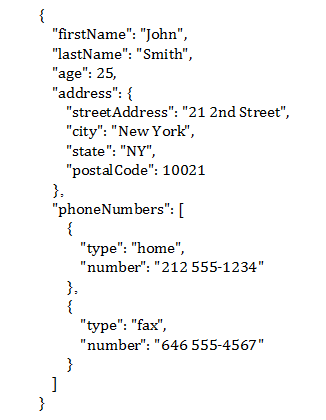
\includegraphics[scale=0.7]{./algorithm/pic/json_example_v1.png}
%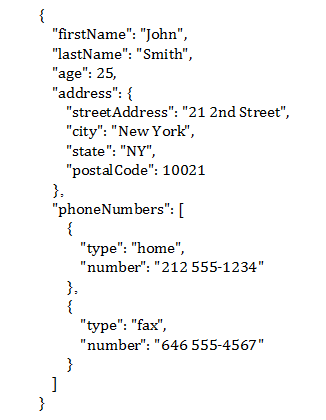
\includegraphics[width=0.4\textwidth]{./algorithm/pic/json_example_v1.png}
\caption{A example of JSON.}
\label{fig:algorithm:json_example}
\end{figure}

\begin{figure}[h]
\centering
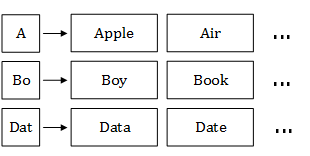
\includegraphics[scale=0.6]{./algorithm/pic/n-gram_v1.png}
%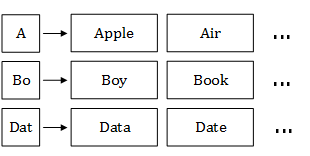
\includegraphics[width=0.4\textwidth]{./algorithm/pic/n-gram_v1.png}
\caption{A example of n-gram indexing.}
\label{fig:algorithm:n-gram}
\end{figure}

Combining all of them can form a special indexing structure which can store the data and query different data type of data, which can very useful for all kind of query and storage system design.\\

Also because Li's Hash is just an algorithm, so it can easily to suit for all kind of key-value stores, or just swap the back-end database that can use another without change any front-end code.\\

%\clearpage

% Data type section
\subsubsection{Data type}

Li's Hash try to fellow KISS (Keep It Simple \& Stupid) principle for user, so Li's Hash will only provide few basic data type to replace the general data type in SQL database \cite{web:mysql:data-types,web:mysql:data-types-store-requirements,web:sqlite:data-types-3,web:transact-sql:data-types}, to decrease the time that user need to understand all kind of data type before writing the code, and can be ignore the range of data type, to let them focus on their system design.\\

The provided data type are \textit{STRING}, \textit{INTEGER}, \textit{REAL}, \textit{BOOLEAN} and \textit{BLOB}. Table \ref{table:algorithm:database-layer:code-example} shows part of data type comparison between Li's Hash and relational database.

Table \ref{table:algorithm:data_type_description} is the description that the storage size and range about each data type.\\

\begin{table}[h]
\centering
\caption{Data type comparison}
\label{table:algorithm:database-layer:code-example}
\begin{tabular}{|c|c|}

\hline
\multicolumn{1}{|c|}{\textbf{Li's Hash}} &
\multicolumn{1}{c|}{\textbf{Relational database}} \\

\hline
\multicolumn{1}{|c|}{STRING} &
\multicolumn{1}{c|}
{\tabincell{c}{
TEXT \\ CHAR \\ VARCHAR
}} \\

\hline
\multicolumn{1}{|c|}{BOOLEAN} &
\multicolumn{1}{c|}
{\tabincell{c}{
CHAR(1) \\ BOOLEAN
}} \\

\hline
\multicolumn{1}{|c|}{BLOB} &
\multicolumn{1}{c|}
{\tabincell{c}{
BLOB
}} \\

\hline
\multicolumn{1}{|c|}{INTEGER} &
\multicolumn{1}{c|}
{\tabincell{c}{
INT \\ INTEGER \\ BIGINT
}} \\

\hline
\multicolumn{1}{|c|}{REAL} &
\multicolumn{1}{c|}
{\tabincell{c}{
REAL \\ DOUBLE \\ FLOAT \\ DECIMAL
}} \\

\hline
\end{tabular}
\end{table}


\begin{table}[h]
\centering
\caption{Data type description}
\label{table:algorithm:data_type_description}
\begin{tabular}{|c|c|c|c|c|c|}

\hline
\multicolumn{1}{|c|}{Type name} &
\multicolumn{1}{c|}{STRING} &
\multicolumn{1}{c|}{BOOLEAN} &
\multicolumn{1}{c|}{INTEGER} &
\multicolumn{1}{c|}{REAL} &
\multicolumn{1}{c|}{BLOB} \\

\hline
\multicolumn{1}{|c|}{indexing} &
\multicolumn{1}{c|}{Y} &
\multicolumn{1}{c|}{Y} &
\multicolumn{1}{c|}{Y} &
\multicolumn{1}{c|}{Y} &
\multicolumn{1}{c|}{N} \\

\hline
\multicolumn{1}{|c|}{byte length (\textit{b})} &
\multicolumn{1}{c|}{dynamic} &
\multicolumn{1}{c|}{1} &
\multicolumn{1}{c|}{8} &
\multicolumn{1}{c|}{dynamic} &
\multicolumn{1}{c|}{dynamic} \\

\hline
\multicolumn{1}{|c|}{data range} &
\multicolumn{1}{c|}{-} &
\multicolumn{1}{c|}{0 $\thicksim$ 1} &
\multicolumn{1}{c|}{
\tabincell{c}
{0 $\thicksim 2^{64}$ - 1 \\ or \\-$2^{63} \thicksim 2^{63}$ - 1}} &
\multicolumn{1}{c|}{No limited} &
\multicolumn{1}{c|}{-} \\

\hline
\end{tabular}
\end{table}

Table \ref{table:algorithm:lishash_type_operation} shows what operation of each data type can do in Li's Hash.

\begin{table}[h]
\centering
\caption{Type of operation}
\label{table:algorithm:lishash_type_operation}
\begin{tabular}{|c|c|c|c|c|c|}

\hline
\multicolumn{1}{|c|}{Type name} &
\multicolumn{1}{c|}{STRING} &
\multicolumn{1}{c|}{BOOLEAN} &
\multicolumn{1}{c|}{INTEGER} &
\multicolumn{1}{c|}{REAL} &
\multicolumn{1}{c|}{BLOB} \\

\hline
\multicolumn{1}{|c|}{\tabincell{c}{Search\\(Exact matching)}} &
\multicolumn{1}{c|}{Y} &
\multicolumn{1}{c|}{Y} &
\multicolumn{1}{c|}{N} &
\multicolumn{1}{c|}{N} &
\multicolumn{1}{c|}{N} \\

\hline
\multicolumn{1}{|c|}{\tabincell{c}{Search\\(Prefix matching)}} &
\multicolumn{1}{c|}{Y} &
\multicolumn{1}{c|}{N} &
\multicolumn{1}{c|}{N} &
\multicolumn{1}{c|}{N} &
\multicolumn{1}{c|}{N} \\

\hline
\multicolumn{1}{|c|}{\tabincell{c}{Search\\(Suffix matching)}} &
\multicolumn{1}{c|}{Y} &
\multicolumn{1}{c|}{N} &
\multicolumn{1}{c|}{N} &
\multicolumn{1}{c|}{N} &
\multicolumn{1}{c|}{N} \\

\hline
\multicolumn{1}{|c|}{\tabincell{c}{Search\\(Partial matching)}} &
\multicolumn{1}{c|}{Y} &
\multicolumn{1}{c|}{N} &
\multicolumn{1}{c|}{N} &
\multicolumn{1}{c|}{N} &
\multicolumn{1}{c|}{N} \\

\hline
\multicolumn{1}{|c|}{Equal} &
\multicolumn{1}{c|}{Y} &
\multicolumn{1}{c|}{Y} &
\multicolumn{1}{c|}{Y} &
\multicolumn{1}{c|}{Y} &
\multicolumn{1}{c|}{N} \\

\hline
\multicolumn{1}{|c|}{\tabincell{c}{Equal\\(muti-value)}} &
\multicolumn{1}{c|}{Y} &
\multicolumn{1}{c|}{Y} &
\multicolumn{1}{c|}{Y} &
\multicolumn{1}{c|}{Y} &
\multicolumn{1}{c|}{N} \\

\hline
\multicolumn{1}{|c|}{Not equal} &
\multicolumn{1}{c|}{Y} &
\multicolumn{1}{c|}{Y} &
\multicolumn{1}{c|}{Y} &
\multicolumn{1}{c|}{Y} &
\multicolumn{1}{c|}{N} \\

\hline
\multicolumn{1}{|c|}{\tabincell{c}{Not equal\\(muti-value)}} &
\multicolumn{1}{c|}{Y} &
\multicolumn{1}{c|}{Y} &
\multicolumn{1}{c|}{Y} &
\multicolumn{1}{c|}{Y} &
\multicolumn{1}{c|}{N} \\

\hline
\multicolumn{1}{|c|}{Less than} &
\multicolumn{1}{c|}{N} &
\multicolumn{1}{c|}{N} &
\multicolumn{1}{c|}{Y} &
\multicolumn{1}{c|}{Y} &
\multicolumn{1}{c|}{N} \\

\hline
\multicolumn{1}{|c|}{Less than or equal} &
\multicolumn{1}{c|}{N} &
\multicolumn{1}{c|}{N} &
\multicolumn{1}{c|}{Y} &
\multicolumn{1}{c|}{Y} &
\multicolumn{1}{c|}{N} \\

\hline
\multicolumn{1}{|c|}{Greater than} &
\multicolumn{1}{c|}{N} &
\multicolumn{1}{c|}{N} &
\multicolumn{1}{c|}{Y} &
\multicolumn{1}{c|}{Y} &
\multicolumn{1}{c|}{N} \\

\hline
\multicolumn{1}{|c|}{Greater than or equal} &
\multicolumn{1}{c|}{N} &
\multicolumn{1}{c|}{N} &
\multicolumn{1}{c|}{Y} &
\multicolumn{1}{c|}{Y} &
\multicolumn{1}{c|}{N} \\

\hline
\multicolumn{1}{|c|}{Between} &
\multicolumn{1}{c|}{N} &
\multicolumn{1}{c|}{N} &
\multicolumn{1}{c|}{Y} &
\multicolumn{1}{c|}{Y} &
\multicolumn{1}{c|}{N} \\

\hline
\end{tabular}
\end{table}

And Table \ref{table:algorithm:data_type_represent_in_sql} is listed the data type will represent that data type in SQL database.

\begin{table}[h]
\centering
\caption{Data type represent in SQL database}
\label{table:algorithm:data_type_represent_in_sql}
\begin{tabular}{|c|c|c|c|c|c|}

\hline
\multicolumn{1}{|c|}{Type} &
\multicolumn{1}{c|}{STRING} &
\multicolumn{1}{c|}{BOOLEAN} &
\multicolumn{1}{c|}{INTEGER} &
\multicolumn{1}{c|}{REAL} &
\multicolumn{1}{c|}{BLOB} \\

\hline
\multicolumn{1}{|c|}{\tabincell{c}{
MySQL\\
\cite{web:mysql:data-types,web:mysql:data-types-store-requirements}
}} &
\multicolumn{1}{c|}{\tabincell{c}{
VARCHAR \\ VARBINARY \\ CHAR \\ BINARY
}} &
\multicolumn{1}{c|}{\tabincell{c}{
CHAR(1) \\ BINARY(1) \\ TINYINT(1)
}} &
\multicolumn{1}{c|}{\tabincell{c}{
TINYINT \\ SMALLINT \\ MEDIUMINT \\ INT \\ INTEGER \\ BIGINT
}} &
\multicolumn{1}{c|}{\tabincell{c}{
FLOAT \\ DOUBLE \\ DECIMAL \\ NUMERIC
}} &
\multicolumn{1}{c|}{\tabincell{c}{
TINYBLOB \\ TINYTEXT \\ BLOB \\ TEXT \\ MEDIUMBLOB \\ MEDIUMTEXT \\ LONGBLOB \\ LONGTEXT
}} \\

\hline
\multicolumn{1}{|c|}{\tabincell{c}{
SQLite\\
\cite{web:sqlite:data-types-3}
}} &
\multicolumn{1}{c|}{\tabincell{c}{
CHARACTER \\ VARCHAR \\ VARYING CHARACTER \\ NCHAR \\ NATIVE CHARACTER \\ NVARCHAR \\ TEXT \\ CLOB
}} &
\multicolumn{1}{c|}{\tabincell{c}{
BOOLEAN
}} &
\multicolumn{1}{c|}{\tabincell{c}{
INT \\ INTEGER \\ TINYINT \\ SMALLINT \\ MEDIUMINT \\ BIGINT \\ UNSIGNED BIG INT \\ INT2 \\ INT8 \\ NUMERIC
}} &
\multicolumn{1}{c|}{\tabincell{c}{
REAL \\ DOUBLE \\ FLOAT
}} &
\multicolumn{1}{c|}{\tabincell{c}{
BLOB
}} \\

\hline
\multicolumn{1}{|c|}{\tabincell{c}{
SQL server\\
\cite{web:transact-sql:data-types}
}} &
\multicolumn{1}{c|}{\tabincell{c}{
char \\ varchar \\ text \\ nchar \\ nvarchar \\ ntext
}} &
\multicolumn{1}{c|}{\tabincell{c}{
bit
}} &
\multicolumn{1}{c|}{\tabincell{c}{
bigint \\ numeric \\ smallint \\ decimal \\ smallmoney \\ int \\ tinyint \\ money
}} &
\multicolumn{1}{c|}{\tabincell{c}{
float \\ real
}} &
\multicolumn{1}{c|}{\tabincell{c}{
binary \\ varbinary \\ image
}} \\

\hline
\end{tabular}
\end{table}

\clearpage

% Index table section
\subsubsection{Index table}

To make the data queryable, Li's Hash design a custom indexing for each data type, so that each data type has their own index tables. The index table is the core concept of Li's Hash. The tables are JSON objects design, there are two kind of index table, \textit{"Index table"} and \textit{"Invert index table"}. Figure \ref{fig:algorithm:lishash_example} is shows the example that the tables looks like contain data \textit{"cow"} with the data type \textit{STRING} which will have more detail later.\\

The tables are using the multi-gram indexing but one table is use the invert way to do the indexing as its name. Because the table is a JSON object, so it is a name-value design, the \textit{"value"} is a collection which means it can store everything no matter an array or a data. In Li's Hash, the \textit{"value"} is pointing to a array which will contain element or data node, but for easy visualization that the array will using a list to show on figure, so call it as \textit{"Bucket"} is quite suitable. This means the index table in Li's Hash as a \textit{"name-bucket"} format.\\

Each element node contain few metadata: the value of this node storing (value), the count of this node is be using (count), and the count of the value repeating (repeat). The data nodes is pointing to the data \textit{id} of the data record.

\begin{figure}[h]
\centering
%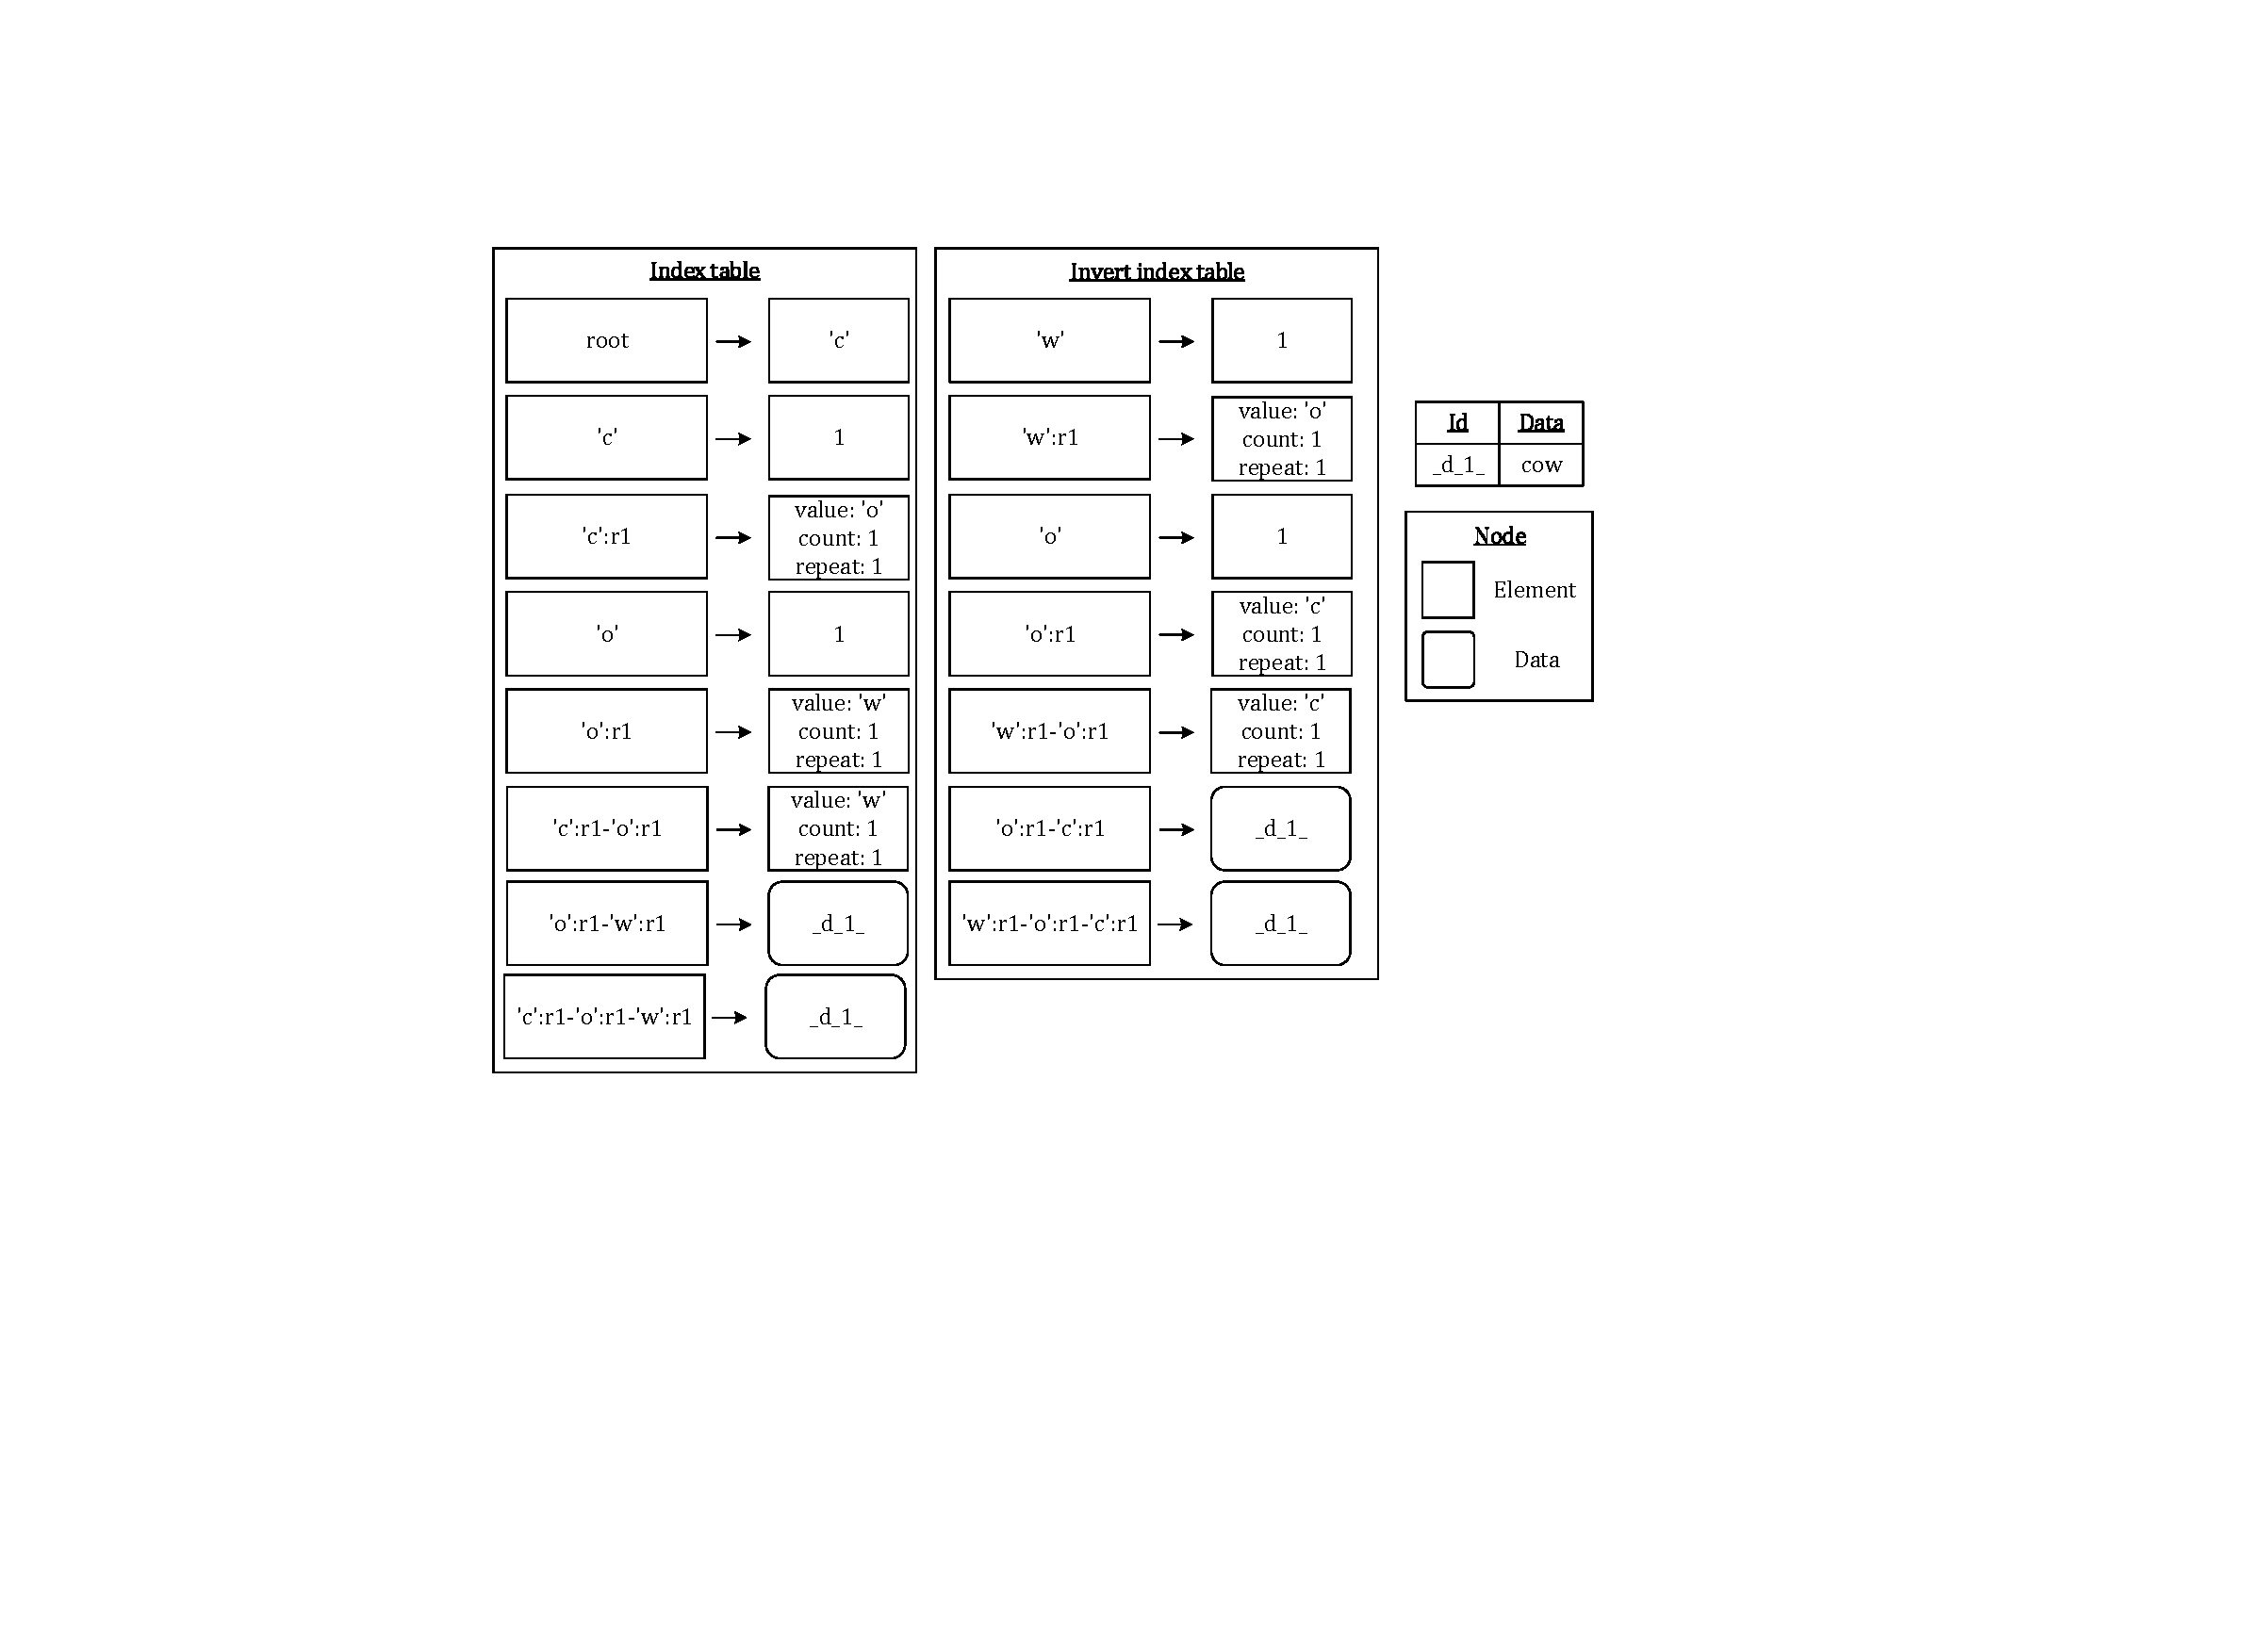
\includegraphics[scale=0.4]{./algorithm/pic/index_table/table_format_v13.pdf}
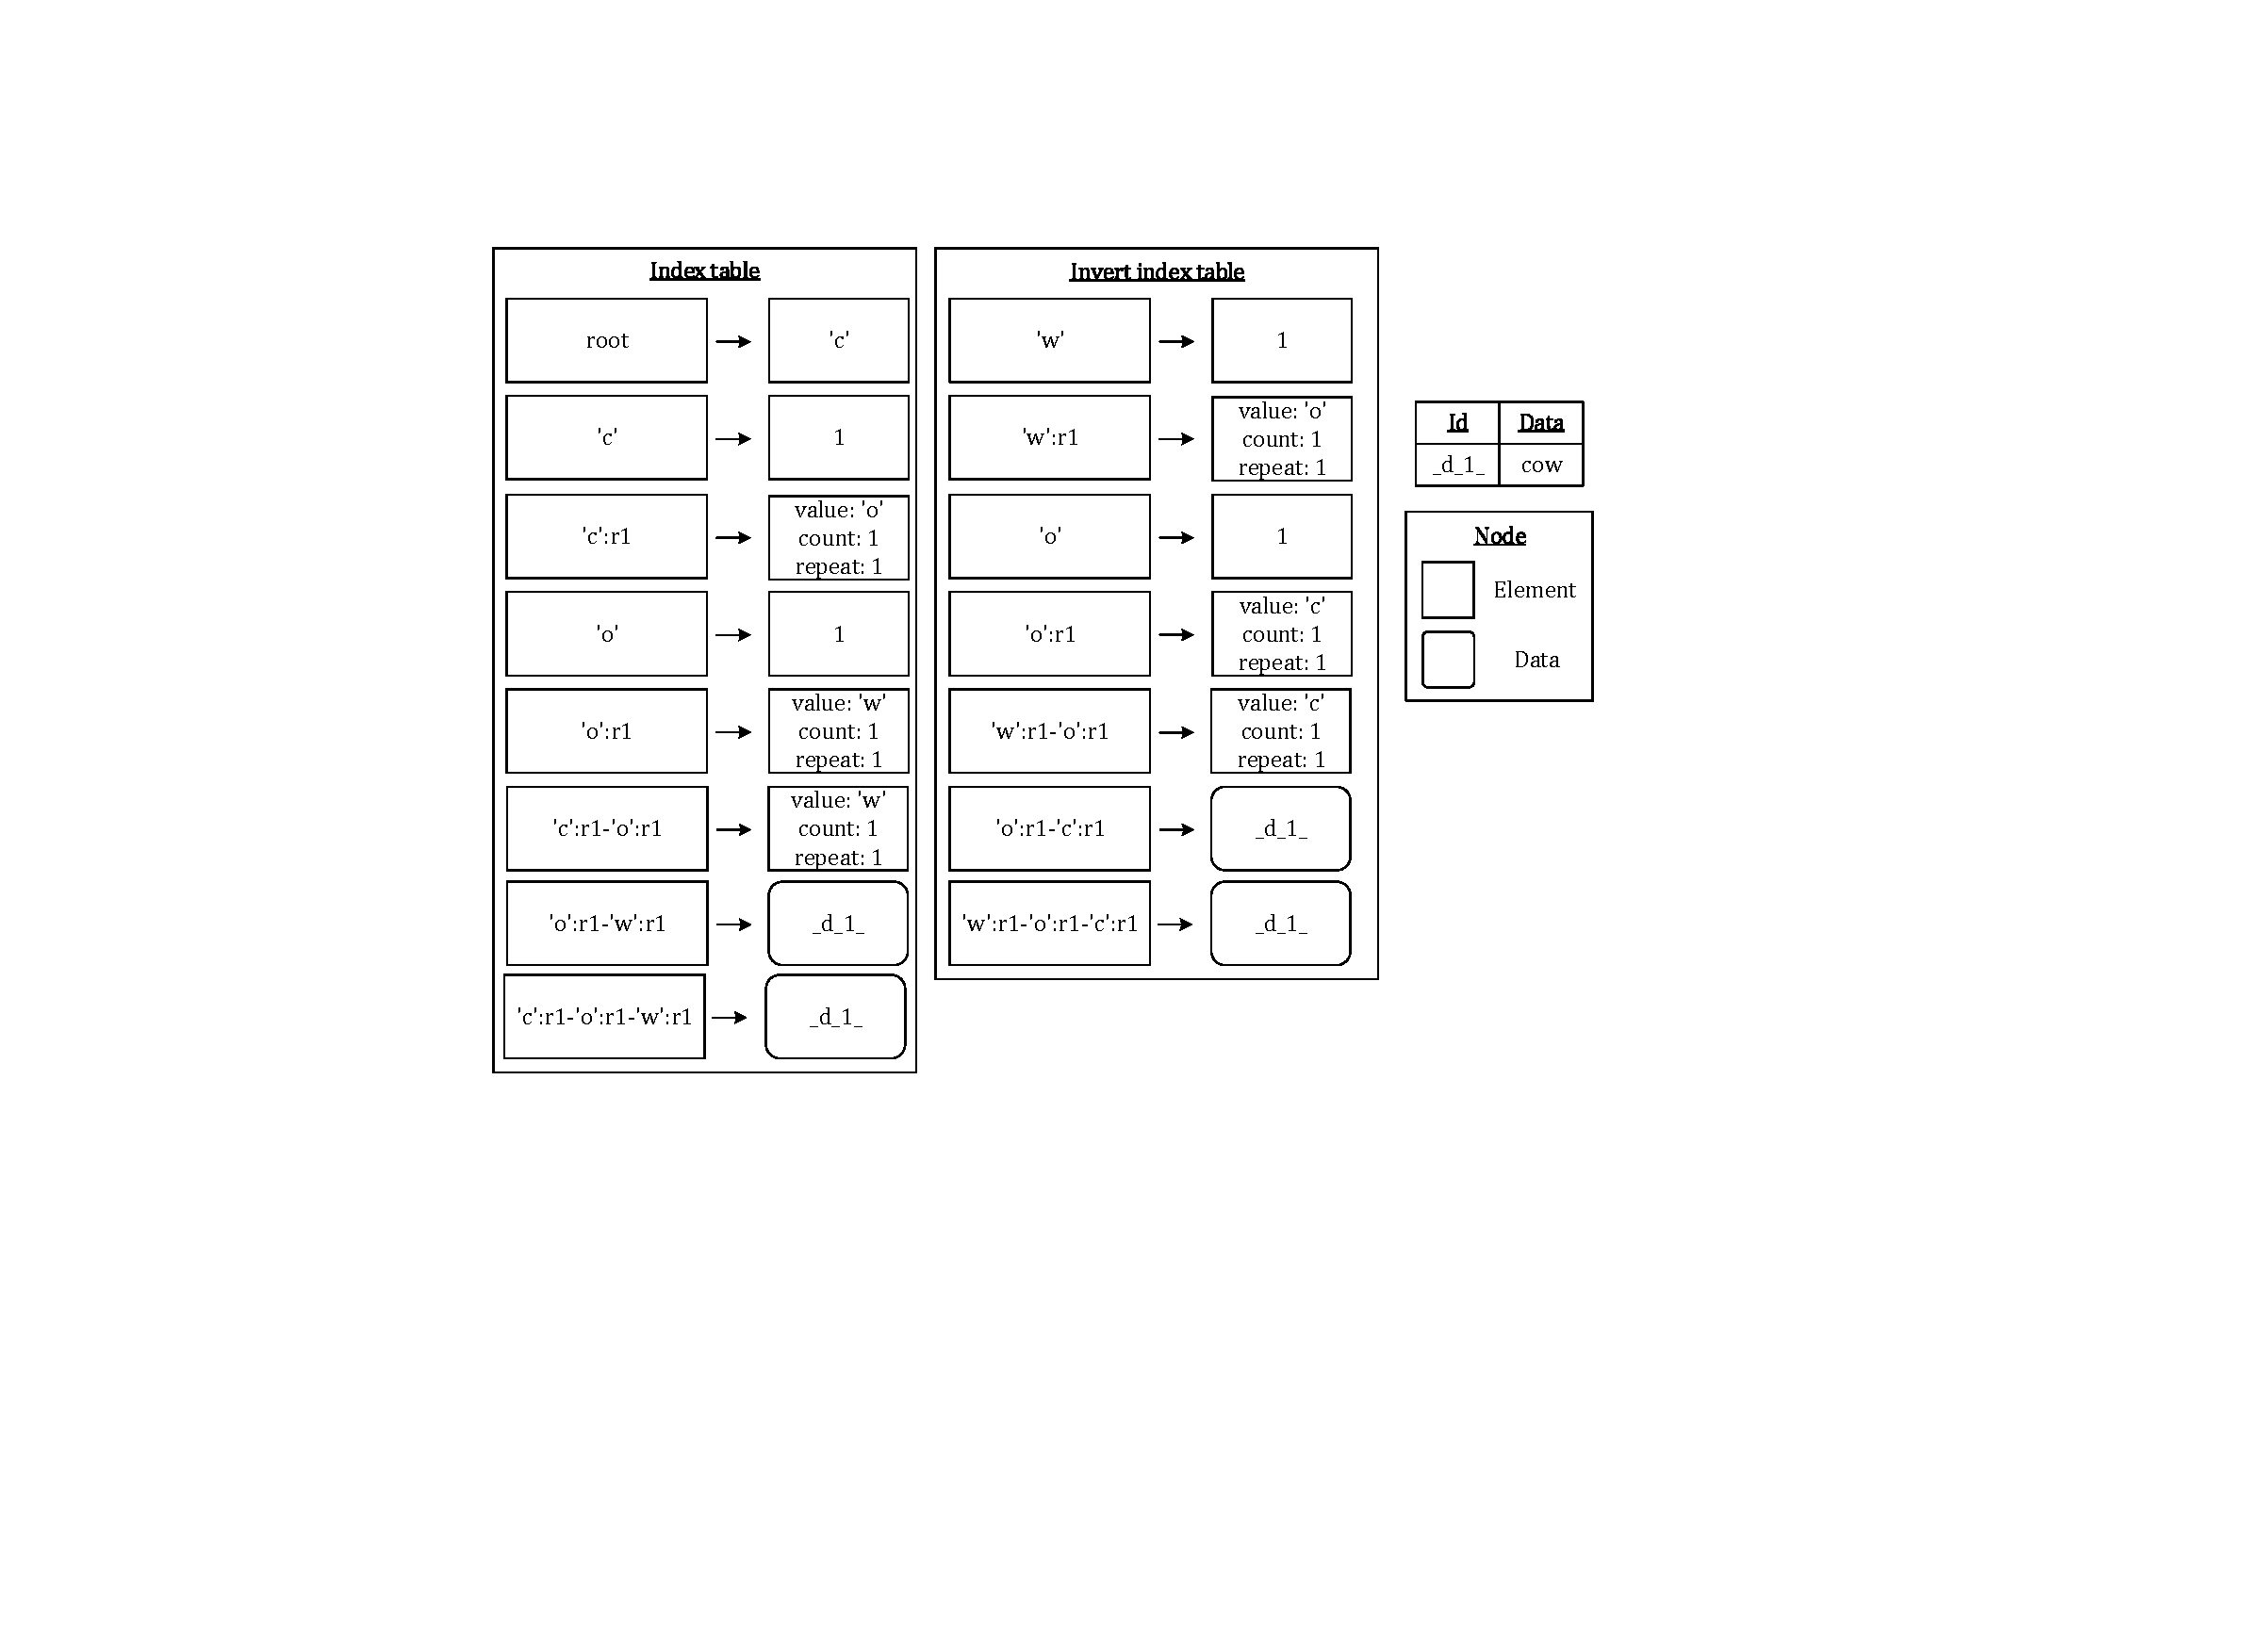
\includegraphics[width=0.8\textwidth]{./algorithm/pic/index_table/table_format_v13.pdf}
\caption{A example of Li's Hash.}
\label{fig:algorithm:lishash_example}
\end{figure}

The time complexity of initial the tables is $O(1)$. About the meanings of all tables, which will more clearly in each operation of all data type.

\clearpage

% STRING section
\subsection{STRING type}

% Insertion section
\subsubsection{Insertion}

When insert a data into the empty table (Figure \ref{fig:algorithm:string:insertion:empty_table}), every data will assign a unique \textit{id} for this data, this \textit{id} will use for the index to look for.

\begin{figure}[h]
\centering
%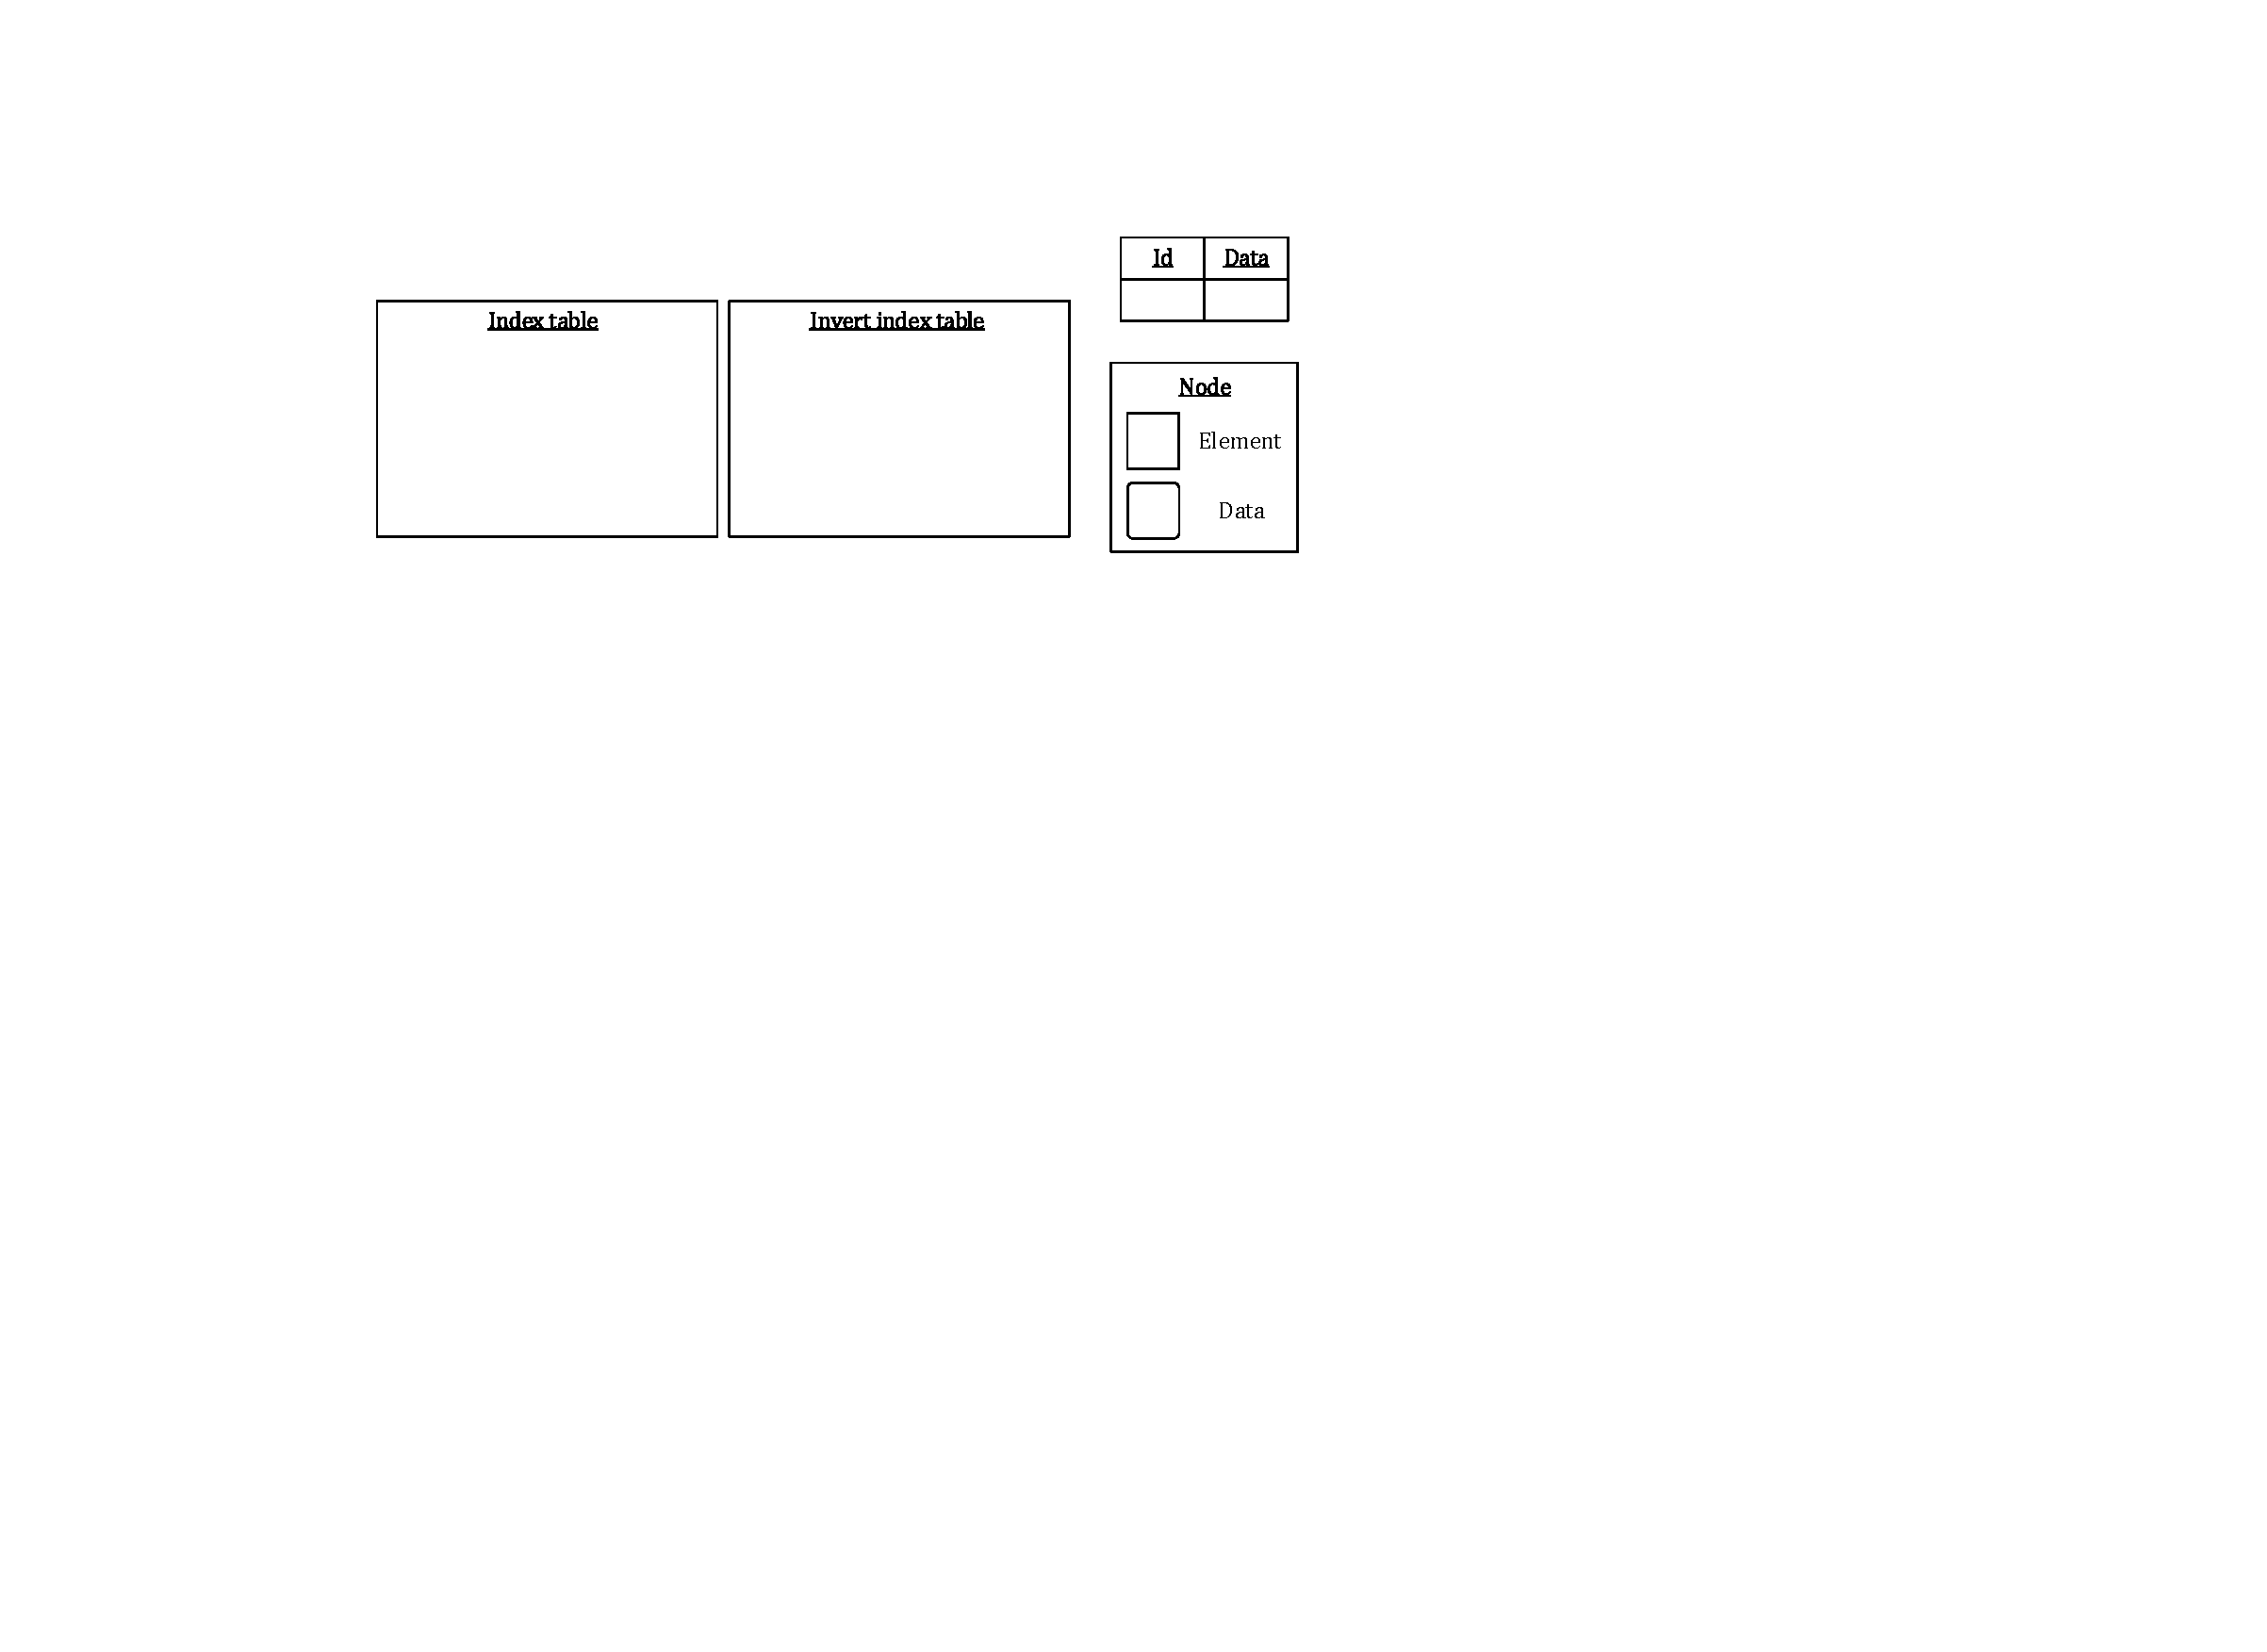
\includegraphics[scale=0.4]{./algorithm/string/pic/insertion/empty_table_v2.pdf}
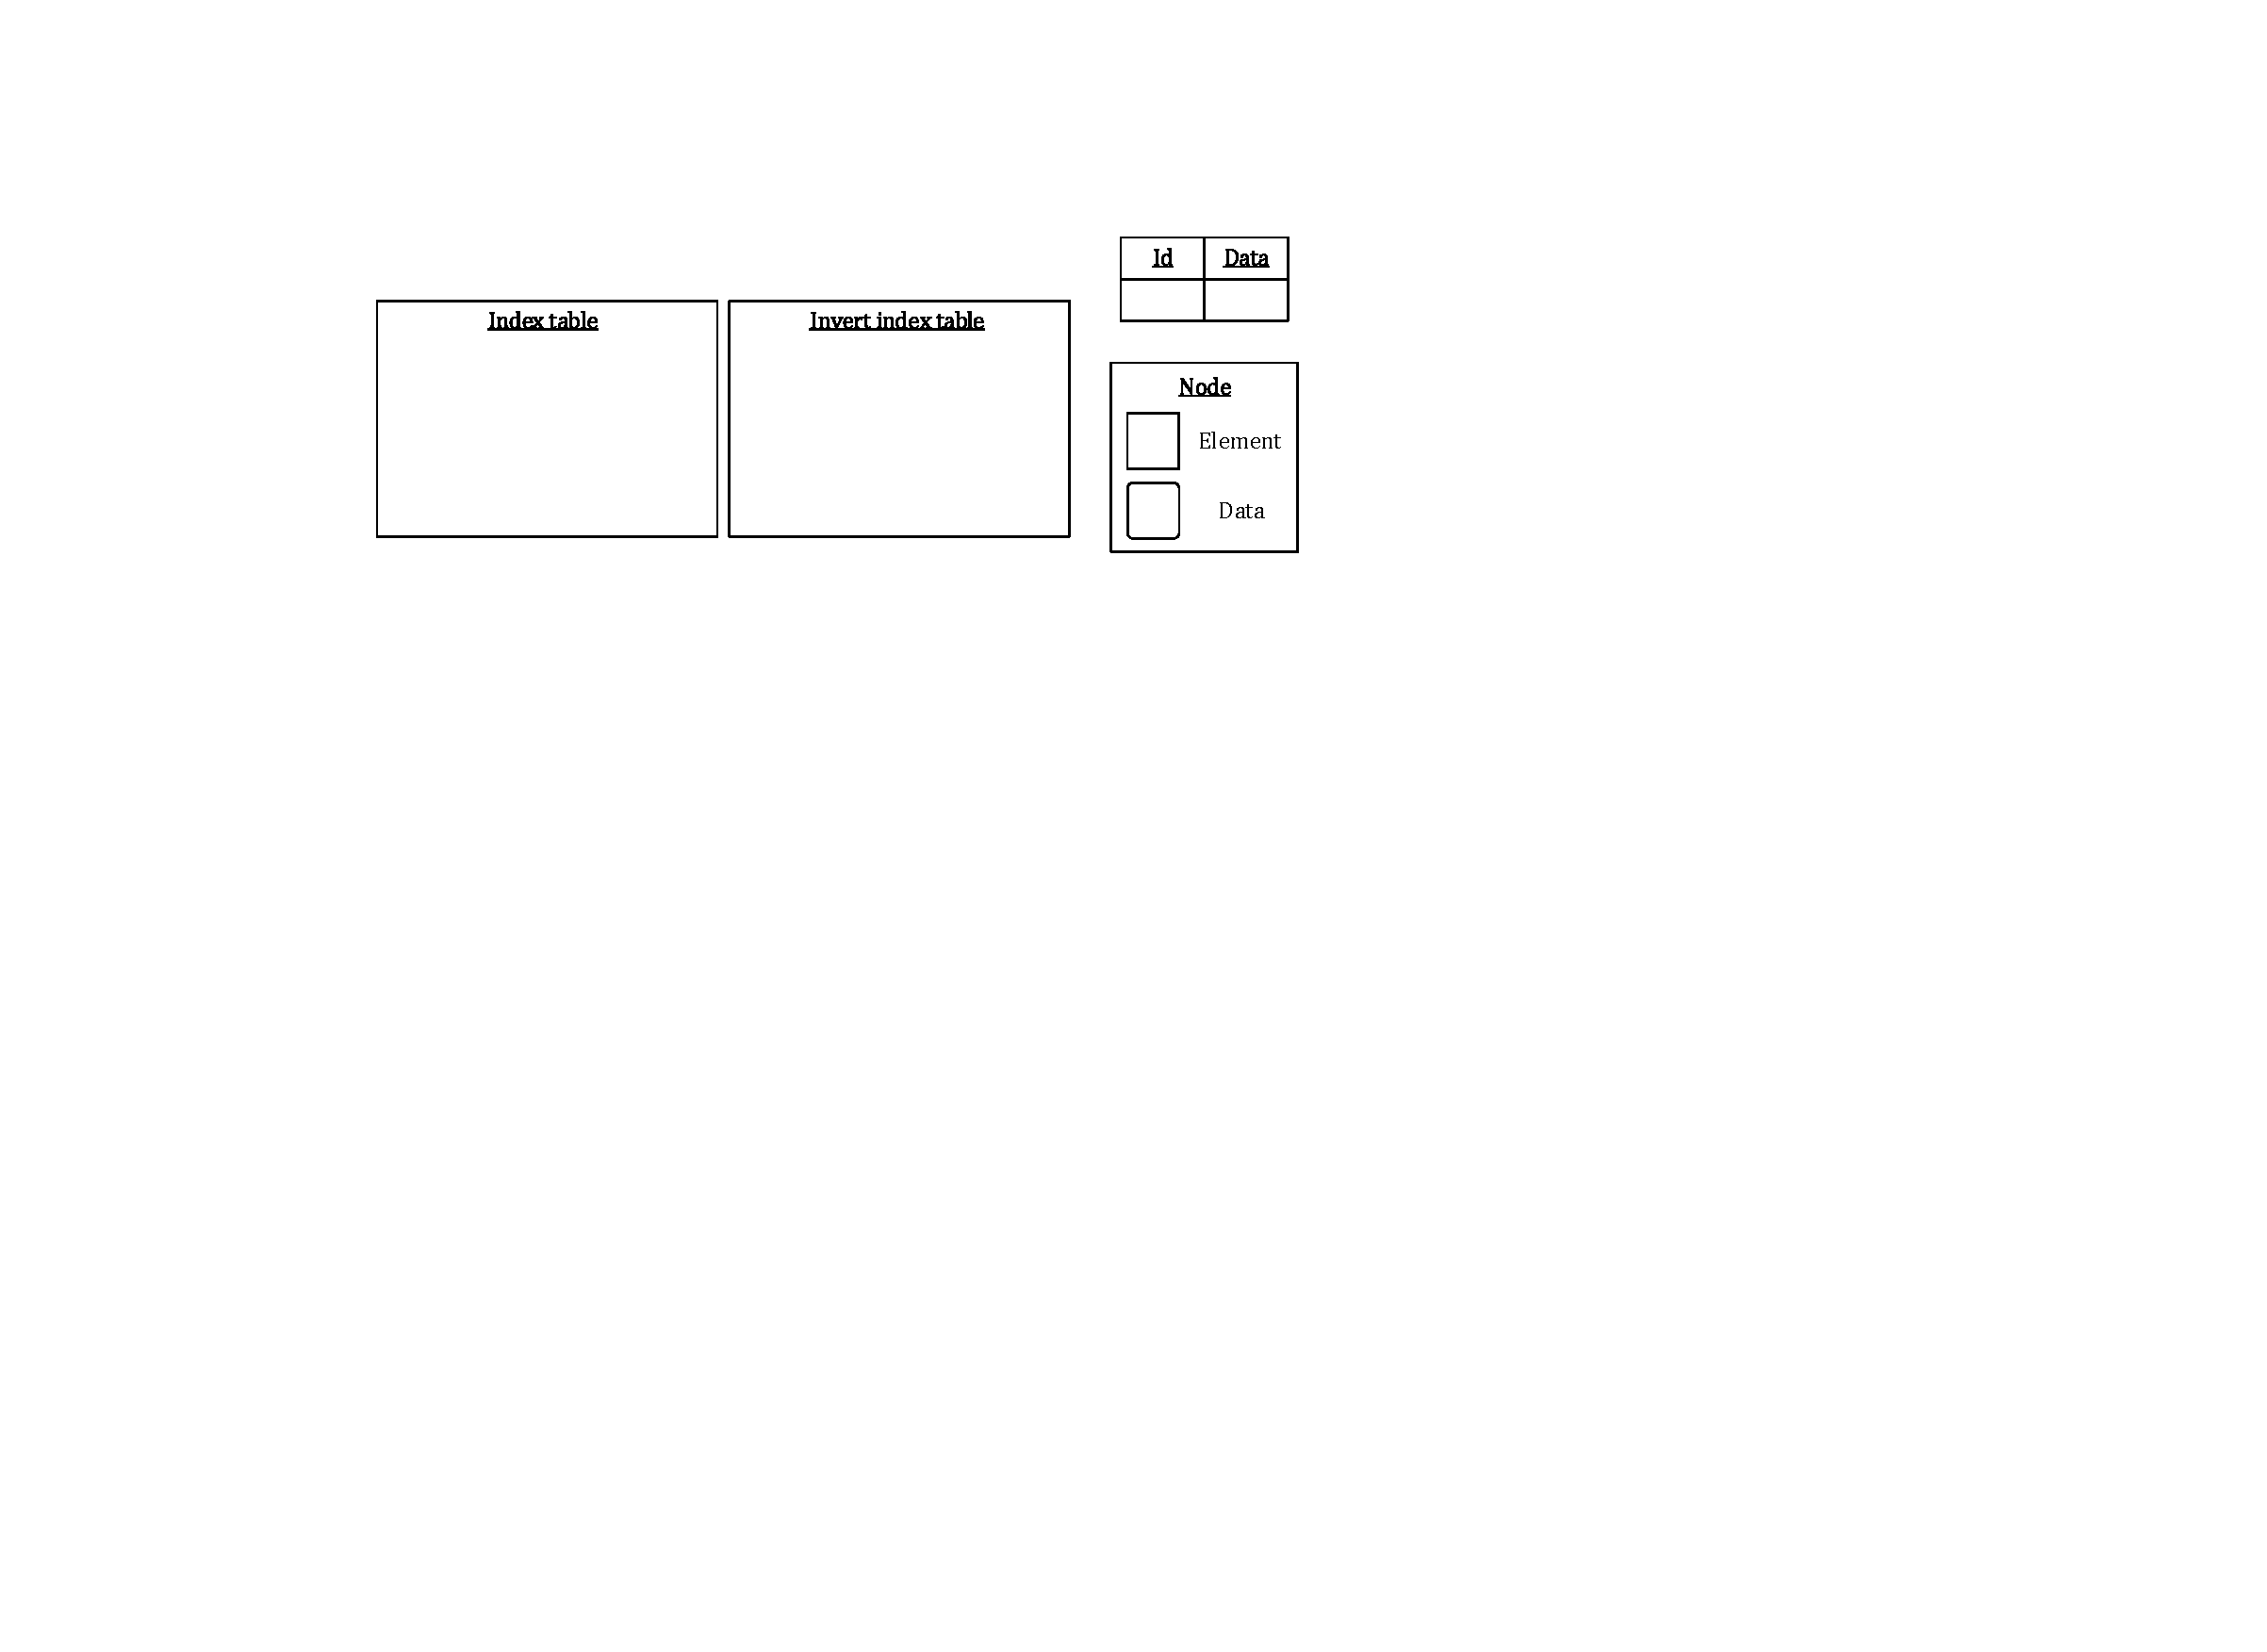
\includegraphics[width=0.5\textwidth]{./algorithm/string/pic/insertion/empty_table_v2.pdf}
\caption{A empty index table.}
\label{fig:algorithm:string:insertion:empty_table}
\end{figure}

So for example if inputting a data \textit{"book"}, first assign the \textit{id} as \textit{"\_d\_1\_"}, next step is separate the bytes using n-gram indexing with counting the repeat value to from the keys. So \textit{"book"} can count as \textit{b-\textgreater1}, \textit{o-\textgreater2} and \textit{k-\textgreater1} by counting the repeat value. And formed into \textit{"b"}, \textit{"bo"}, \textit{"boo"}, \textit{"book"}, \textit{"oo"}, \textit{"ook"} by n-gram but because using count the repeat byte that \textit{"bo"} is domained by \textit{"boo"}.\\

Every byte will have their own key such as \textit{'b'} and \textit{'o'} for record their repeat count, which is using in searching to know there have the keys like \textit{"'b':r1"} or \textit{"'o':r2"} which can use. The \textit{'r'} in key means the repeat times of that value. But the last byte wouldn't have that key in index table because of the key will exist in invert index table, also this happen in the opposite.\\

So the data will index as figure \ref{fig:algorithm:string:insertion:example_1}.

\begin{figure}[h]
\centering
%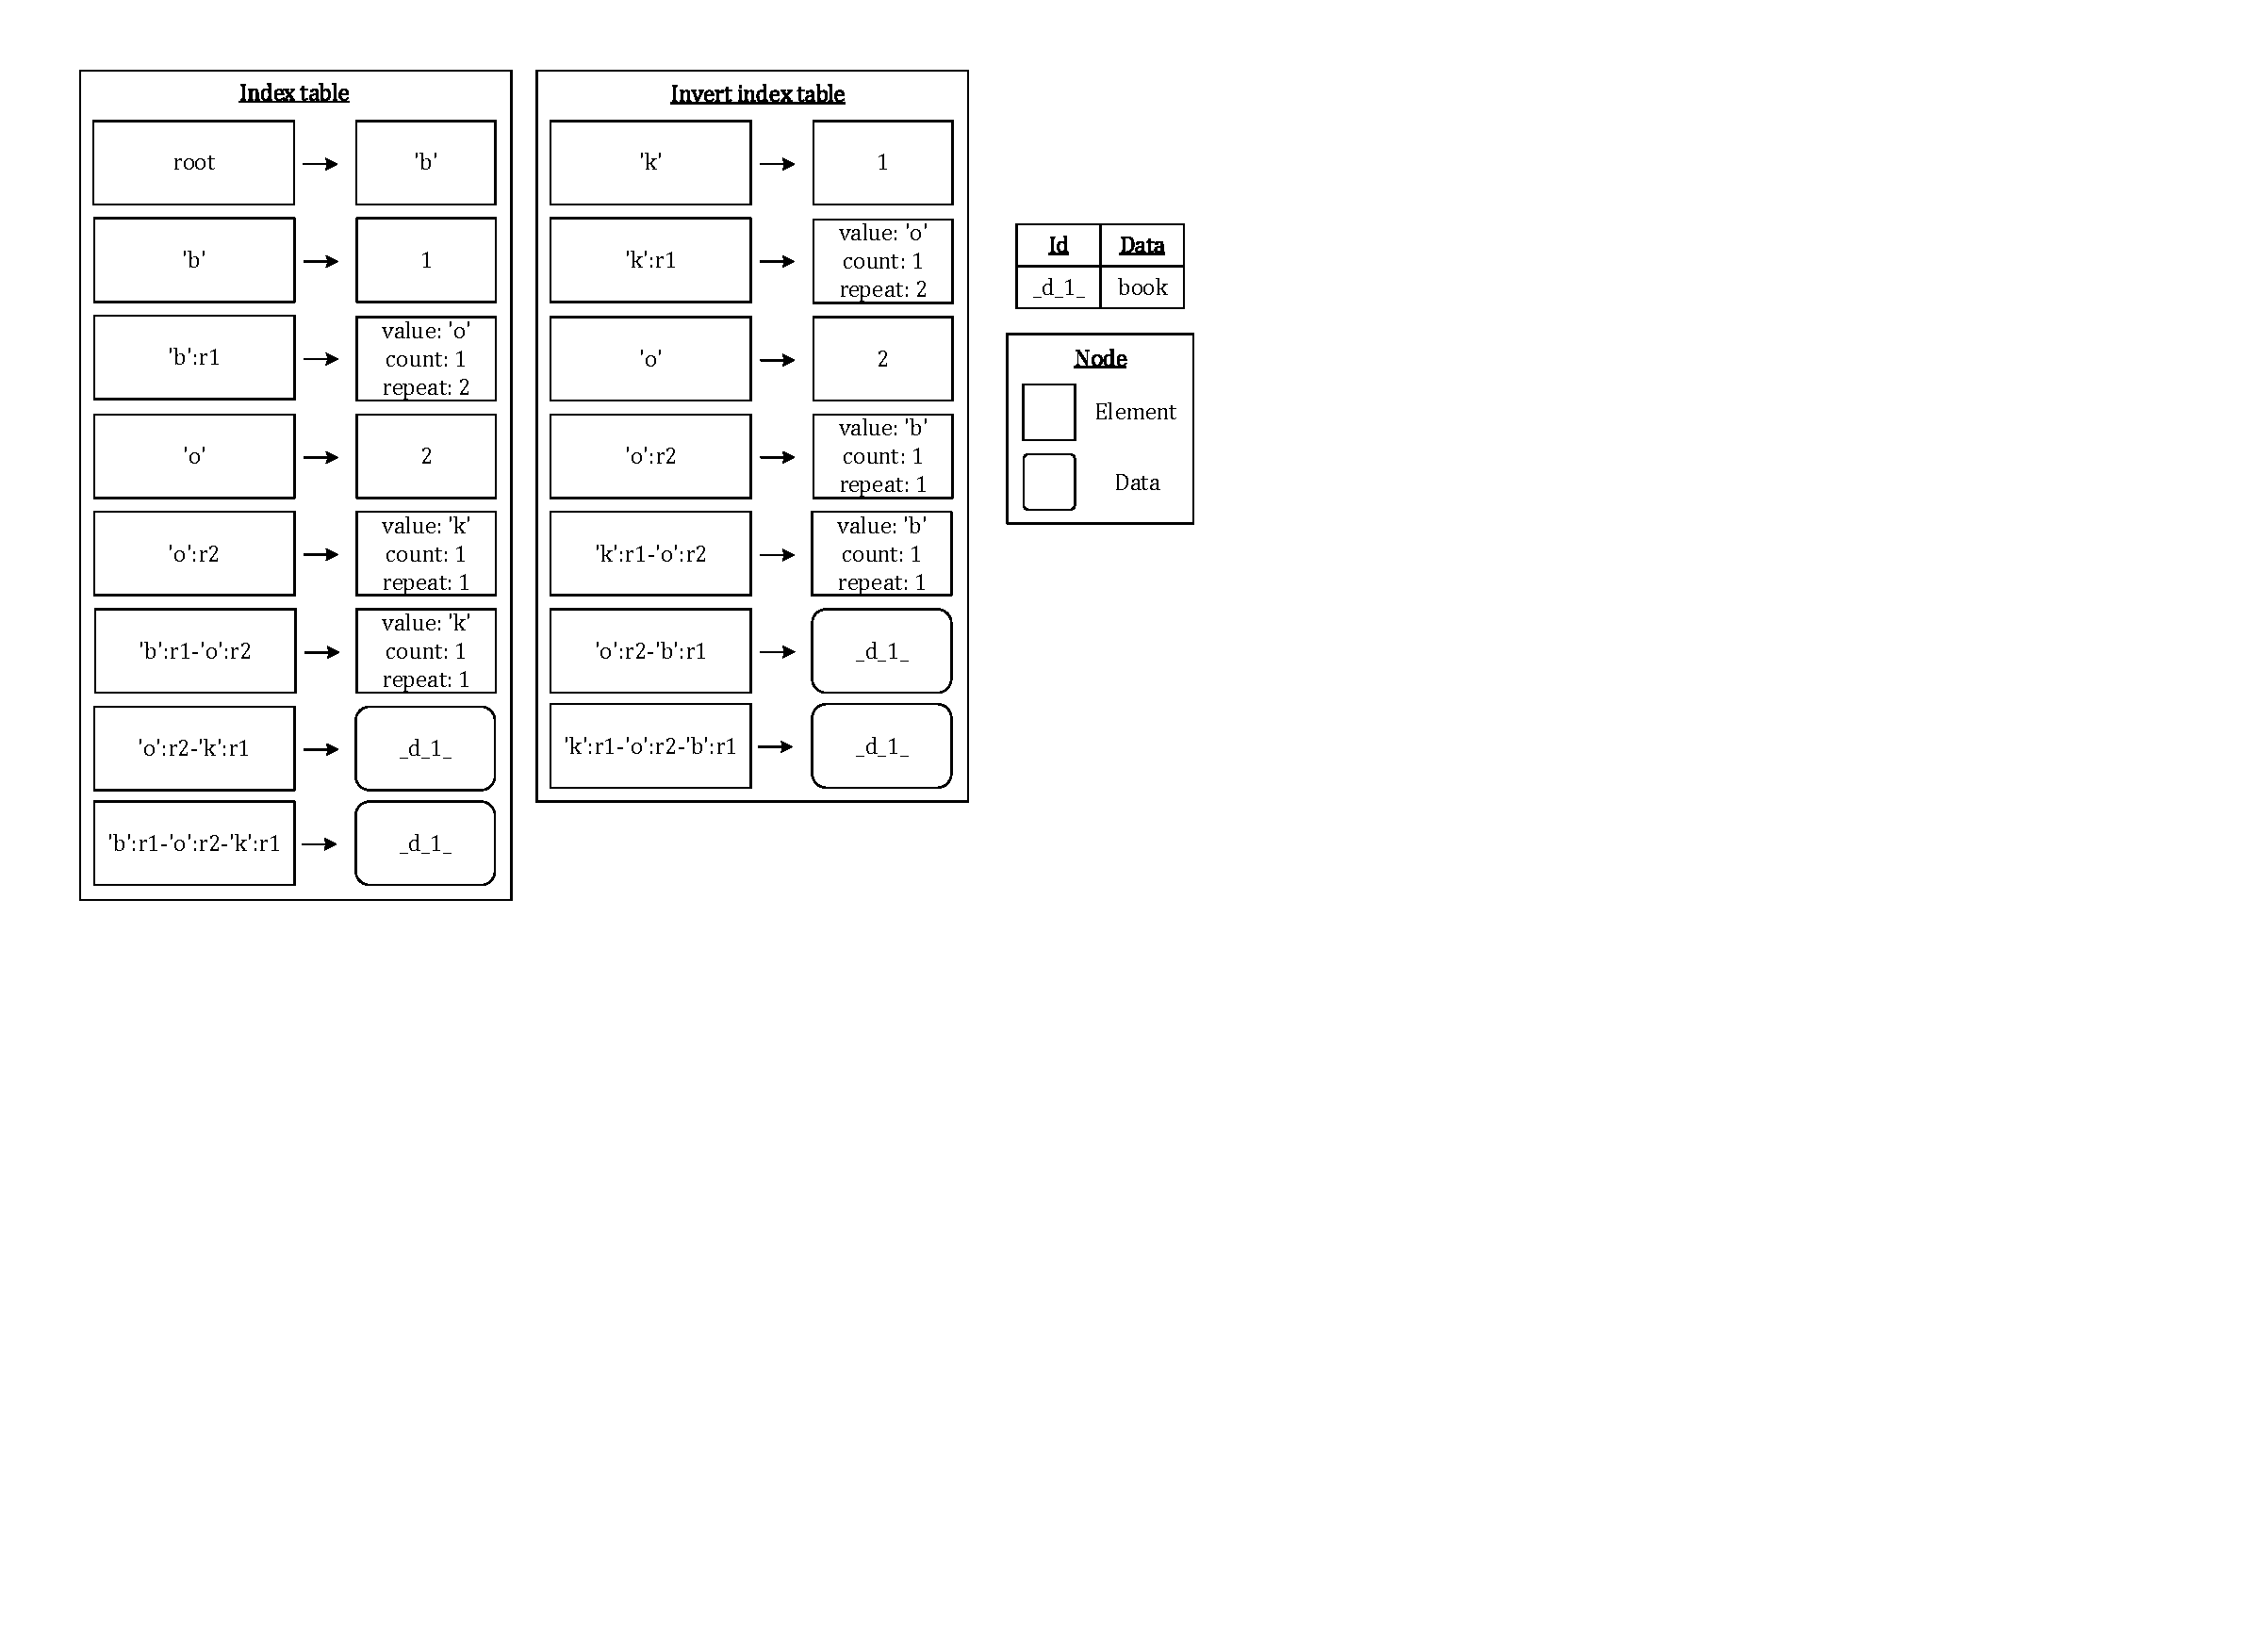
\includegraphics[scale=1.0]{./algorithm/string/pic/insertion/example_1_v5.pdf}
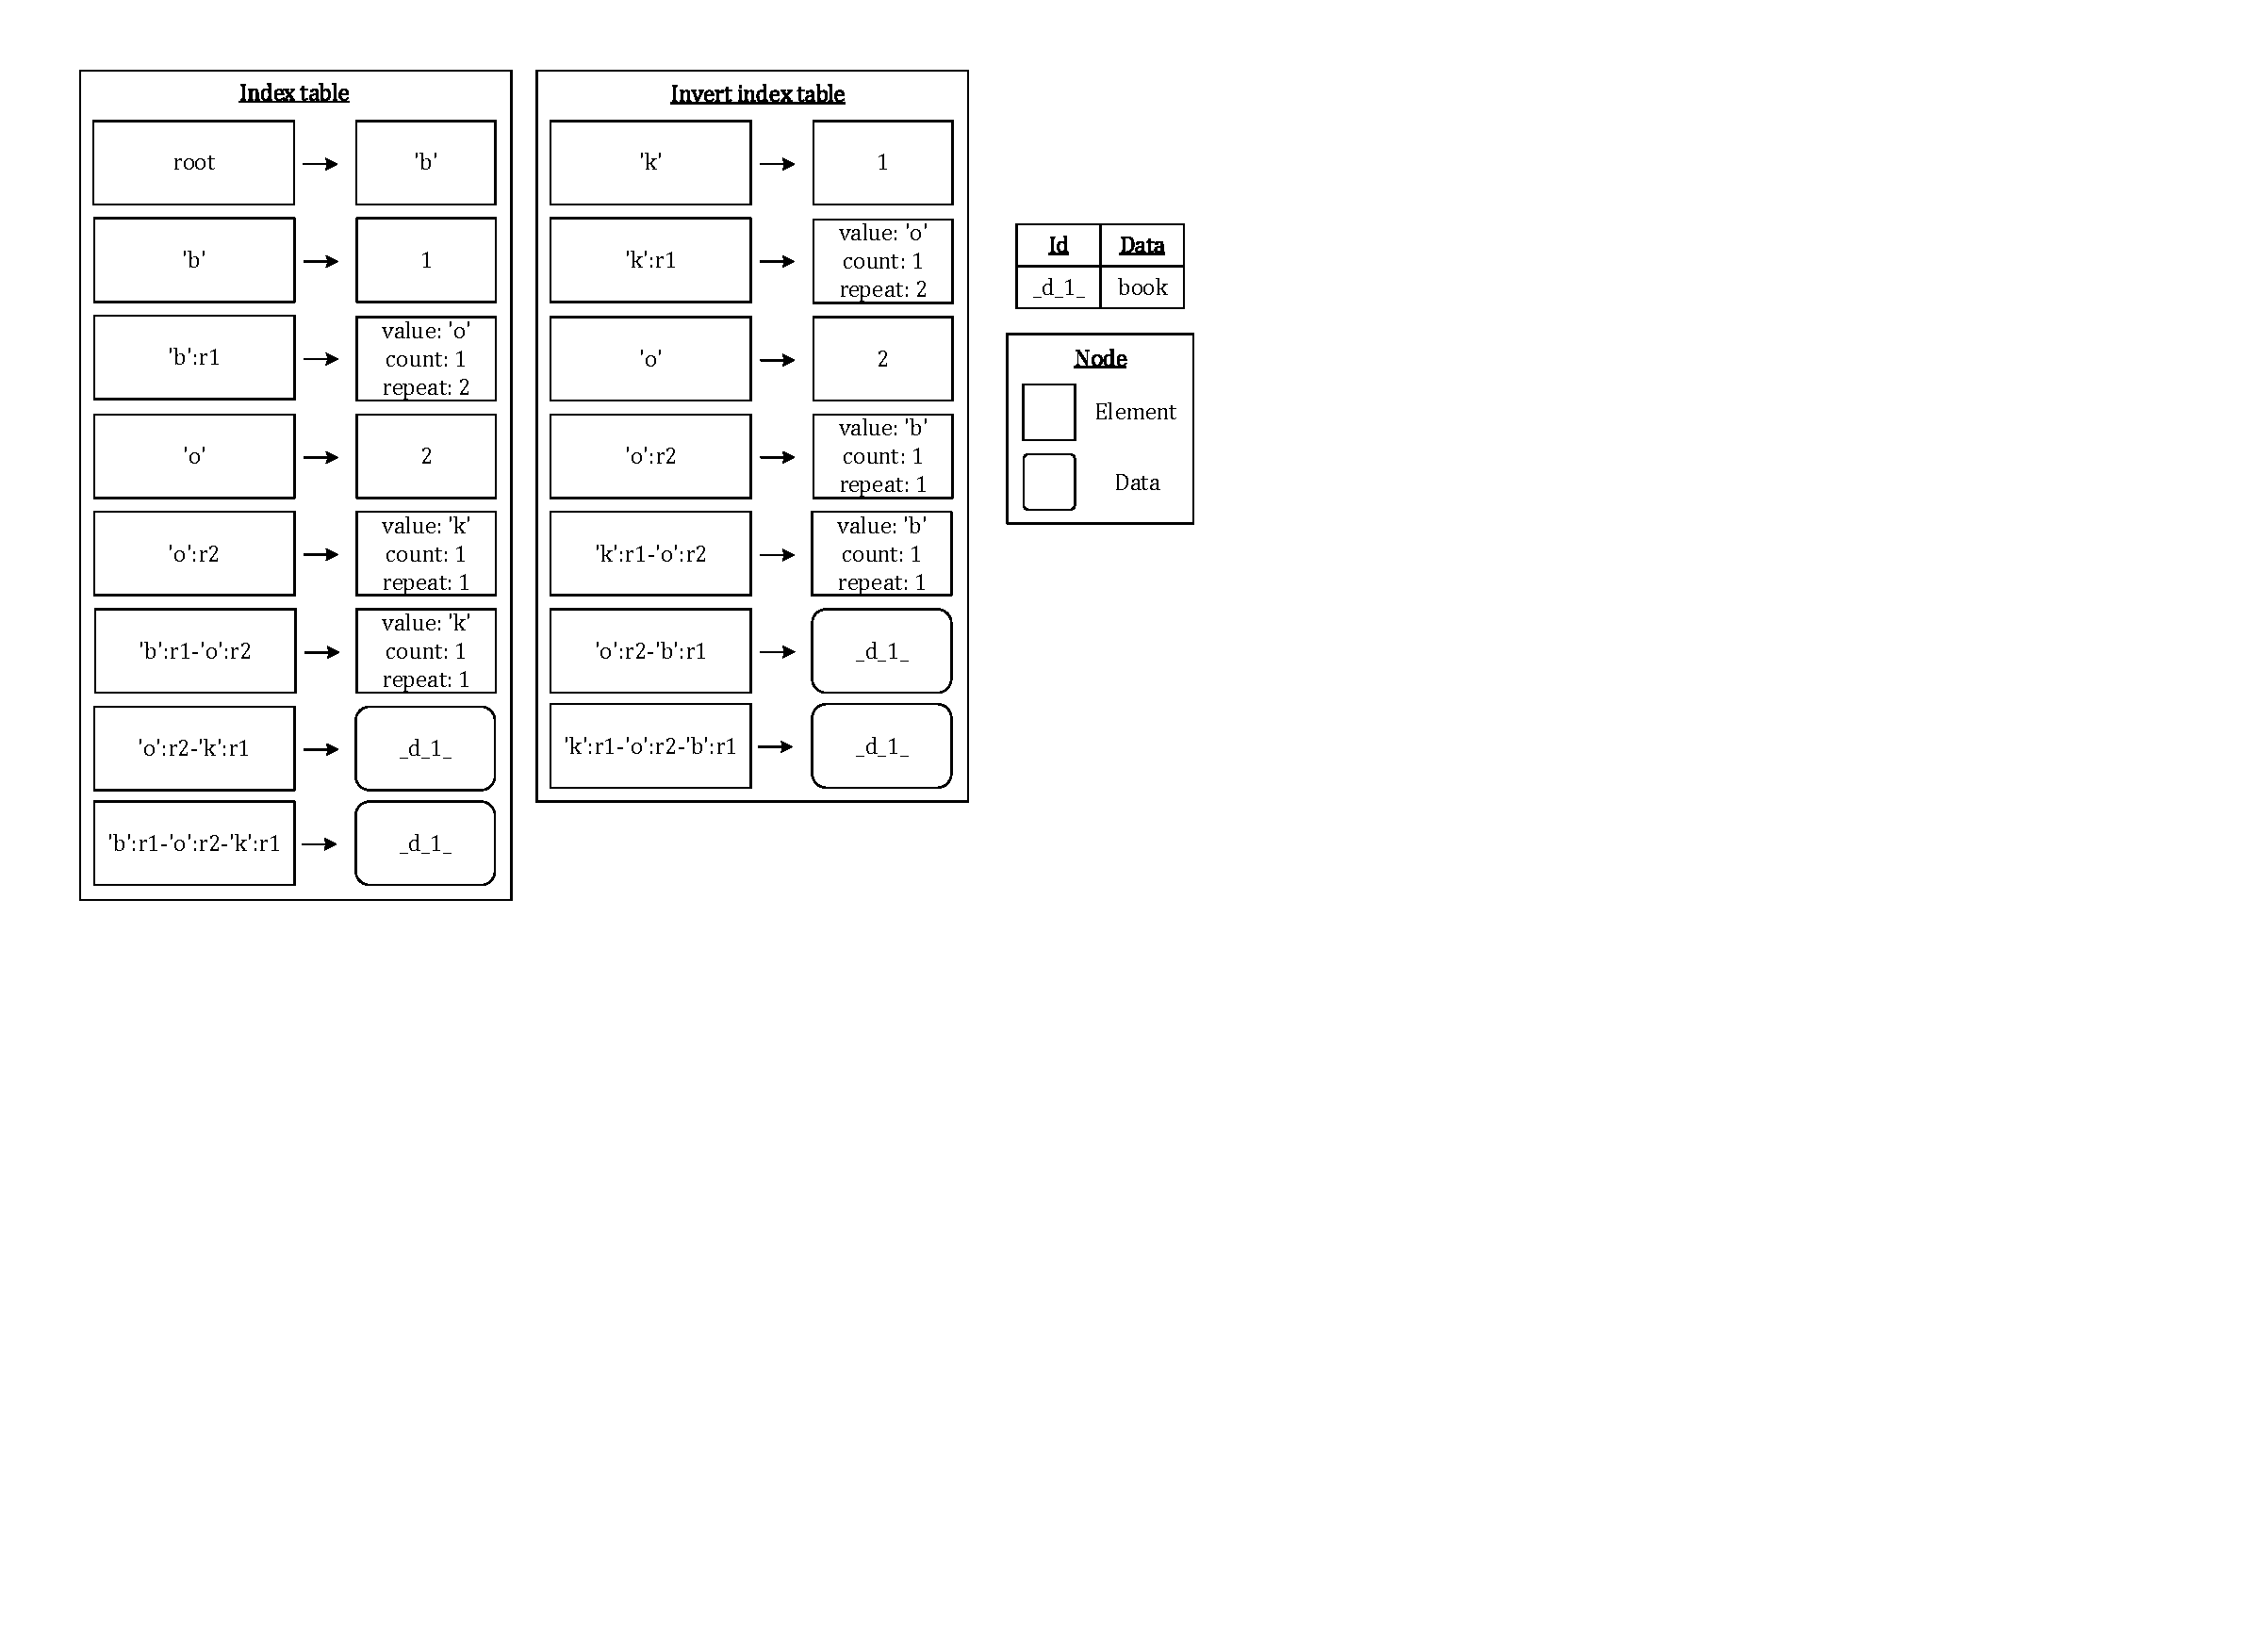
\includegraphics[width=0.7\textwidth]{./algorithm/string/pic/insertion/example_1_v5.pdf}
\caption{Insert data "book".}
\label{fig:algorithm:string:insertion:example_1}
\end{figure}

The time complexity of insertion should look like figure \ref{fig:algorithm:string:insertion:time_complexity}. The time complexity of insert a data should be $O(b)$, $b!$ is the number of for loop which is equal to the byte length of data, and $O(1)$ is means the key of the data like \textit{"'b':r1-'o':r2-'k':r1"} in the example.\\

\begin{figure}[h]
\centering
%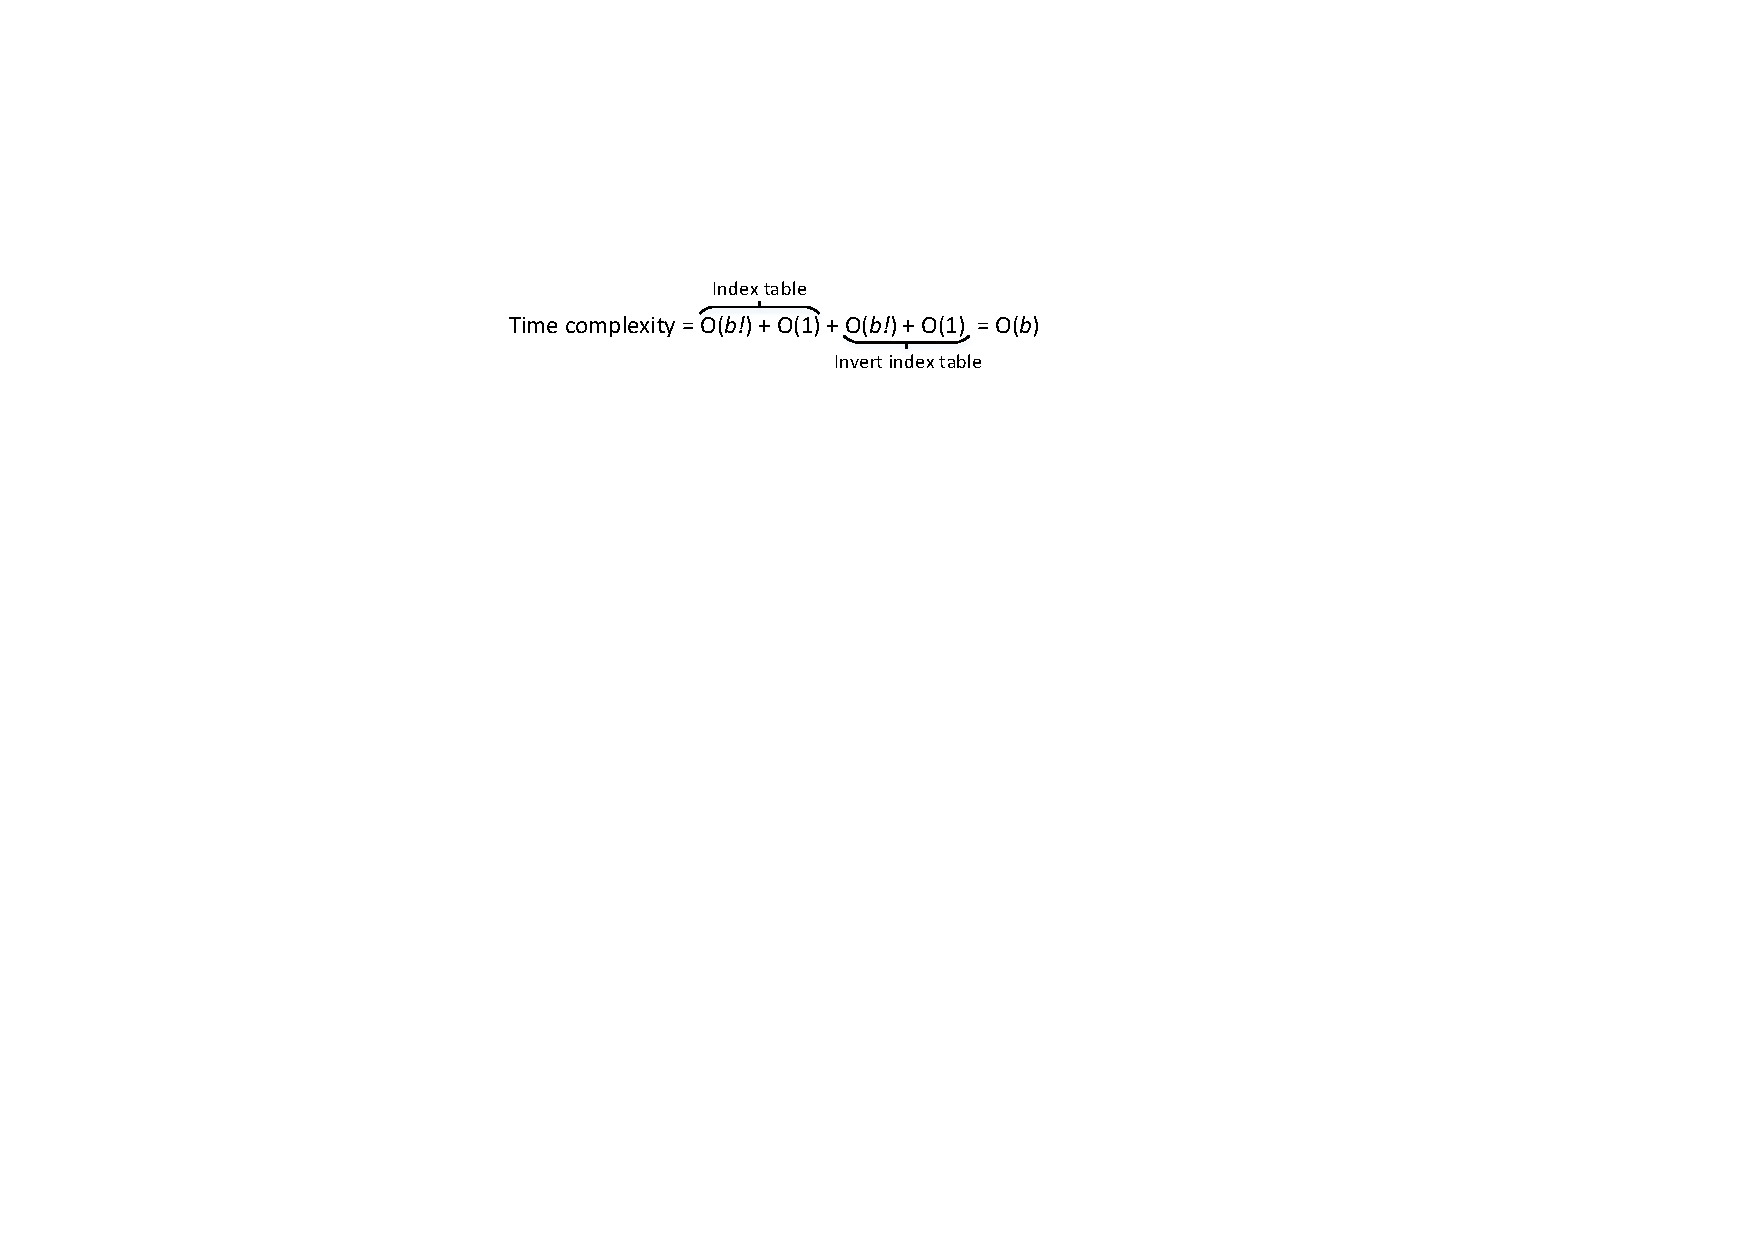
\includegraphics[scale=1.0]{./algorithm/string/pic/insertion/time_complexity_v5.pdf}
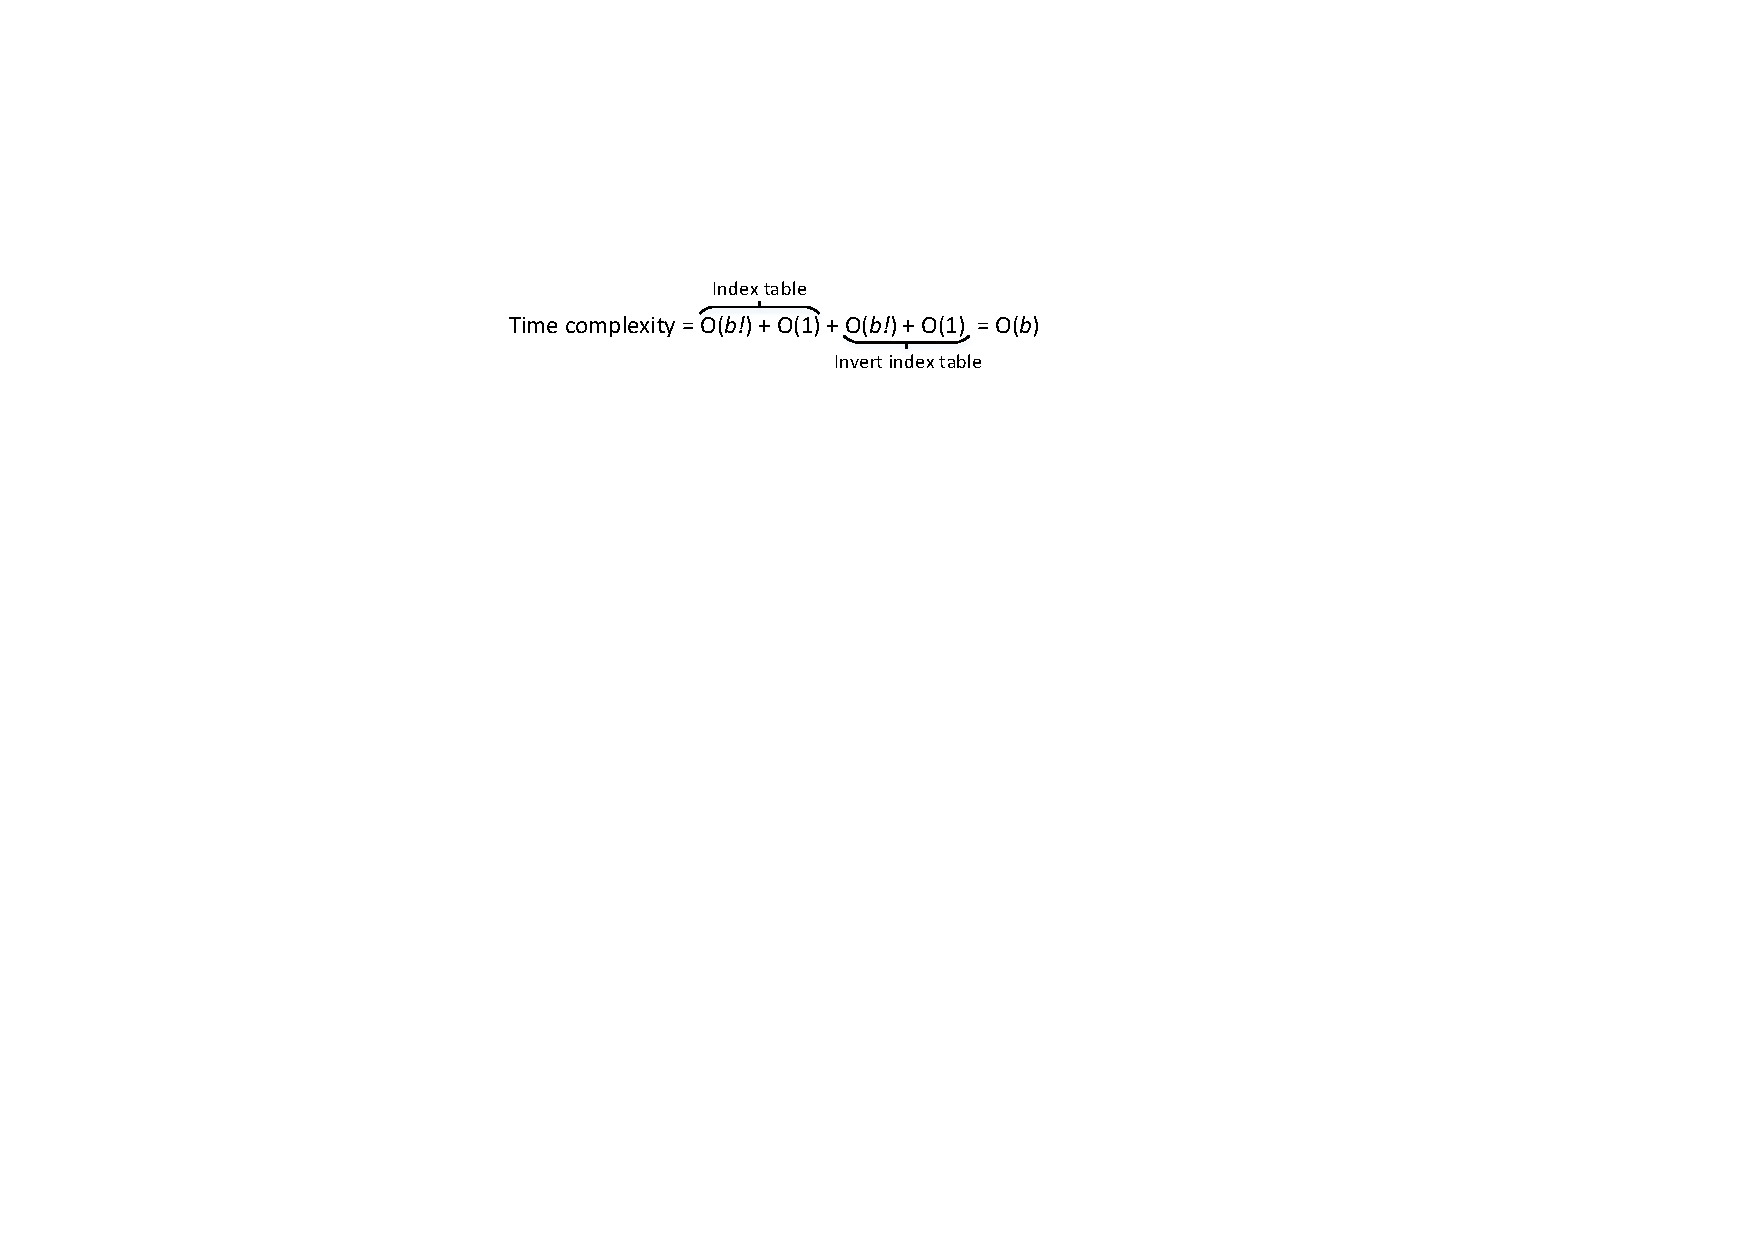
\includegraphics[width=0.6\textwidth]{./algorithm/string/pic/insertion/time_complexity_v5.pdf}
\caption{Time complexity of insertion.}
\label{fig:algorithm:string:insertion:time_complexity}
\end{figure}

Next if insert the data \textit{"box"}, the tables will look like figure \ref{fig:algorithm:string:insertion:example_2}. As the figure shows that \textit{"box"} and \textit{"book"} have a common key, so some of the node will deduplicated.

\begin{figure}[h]
\centering
%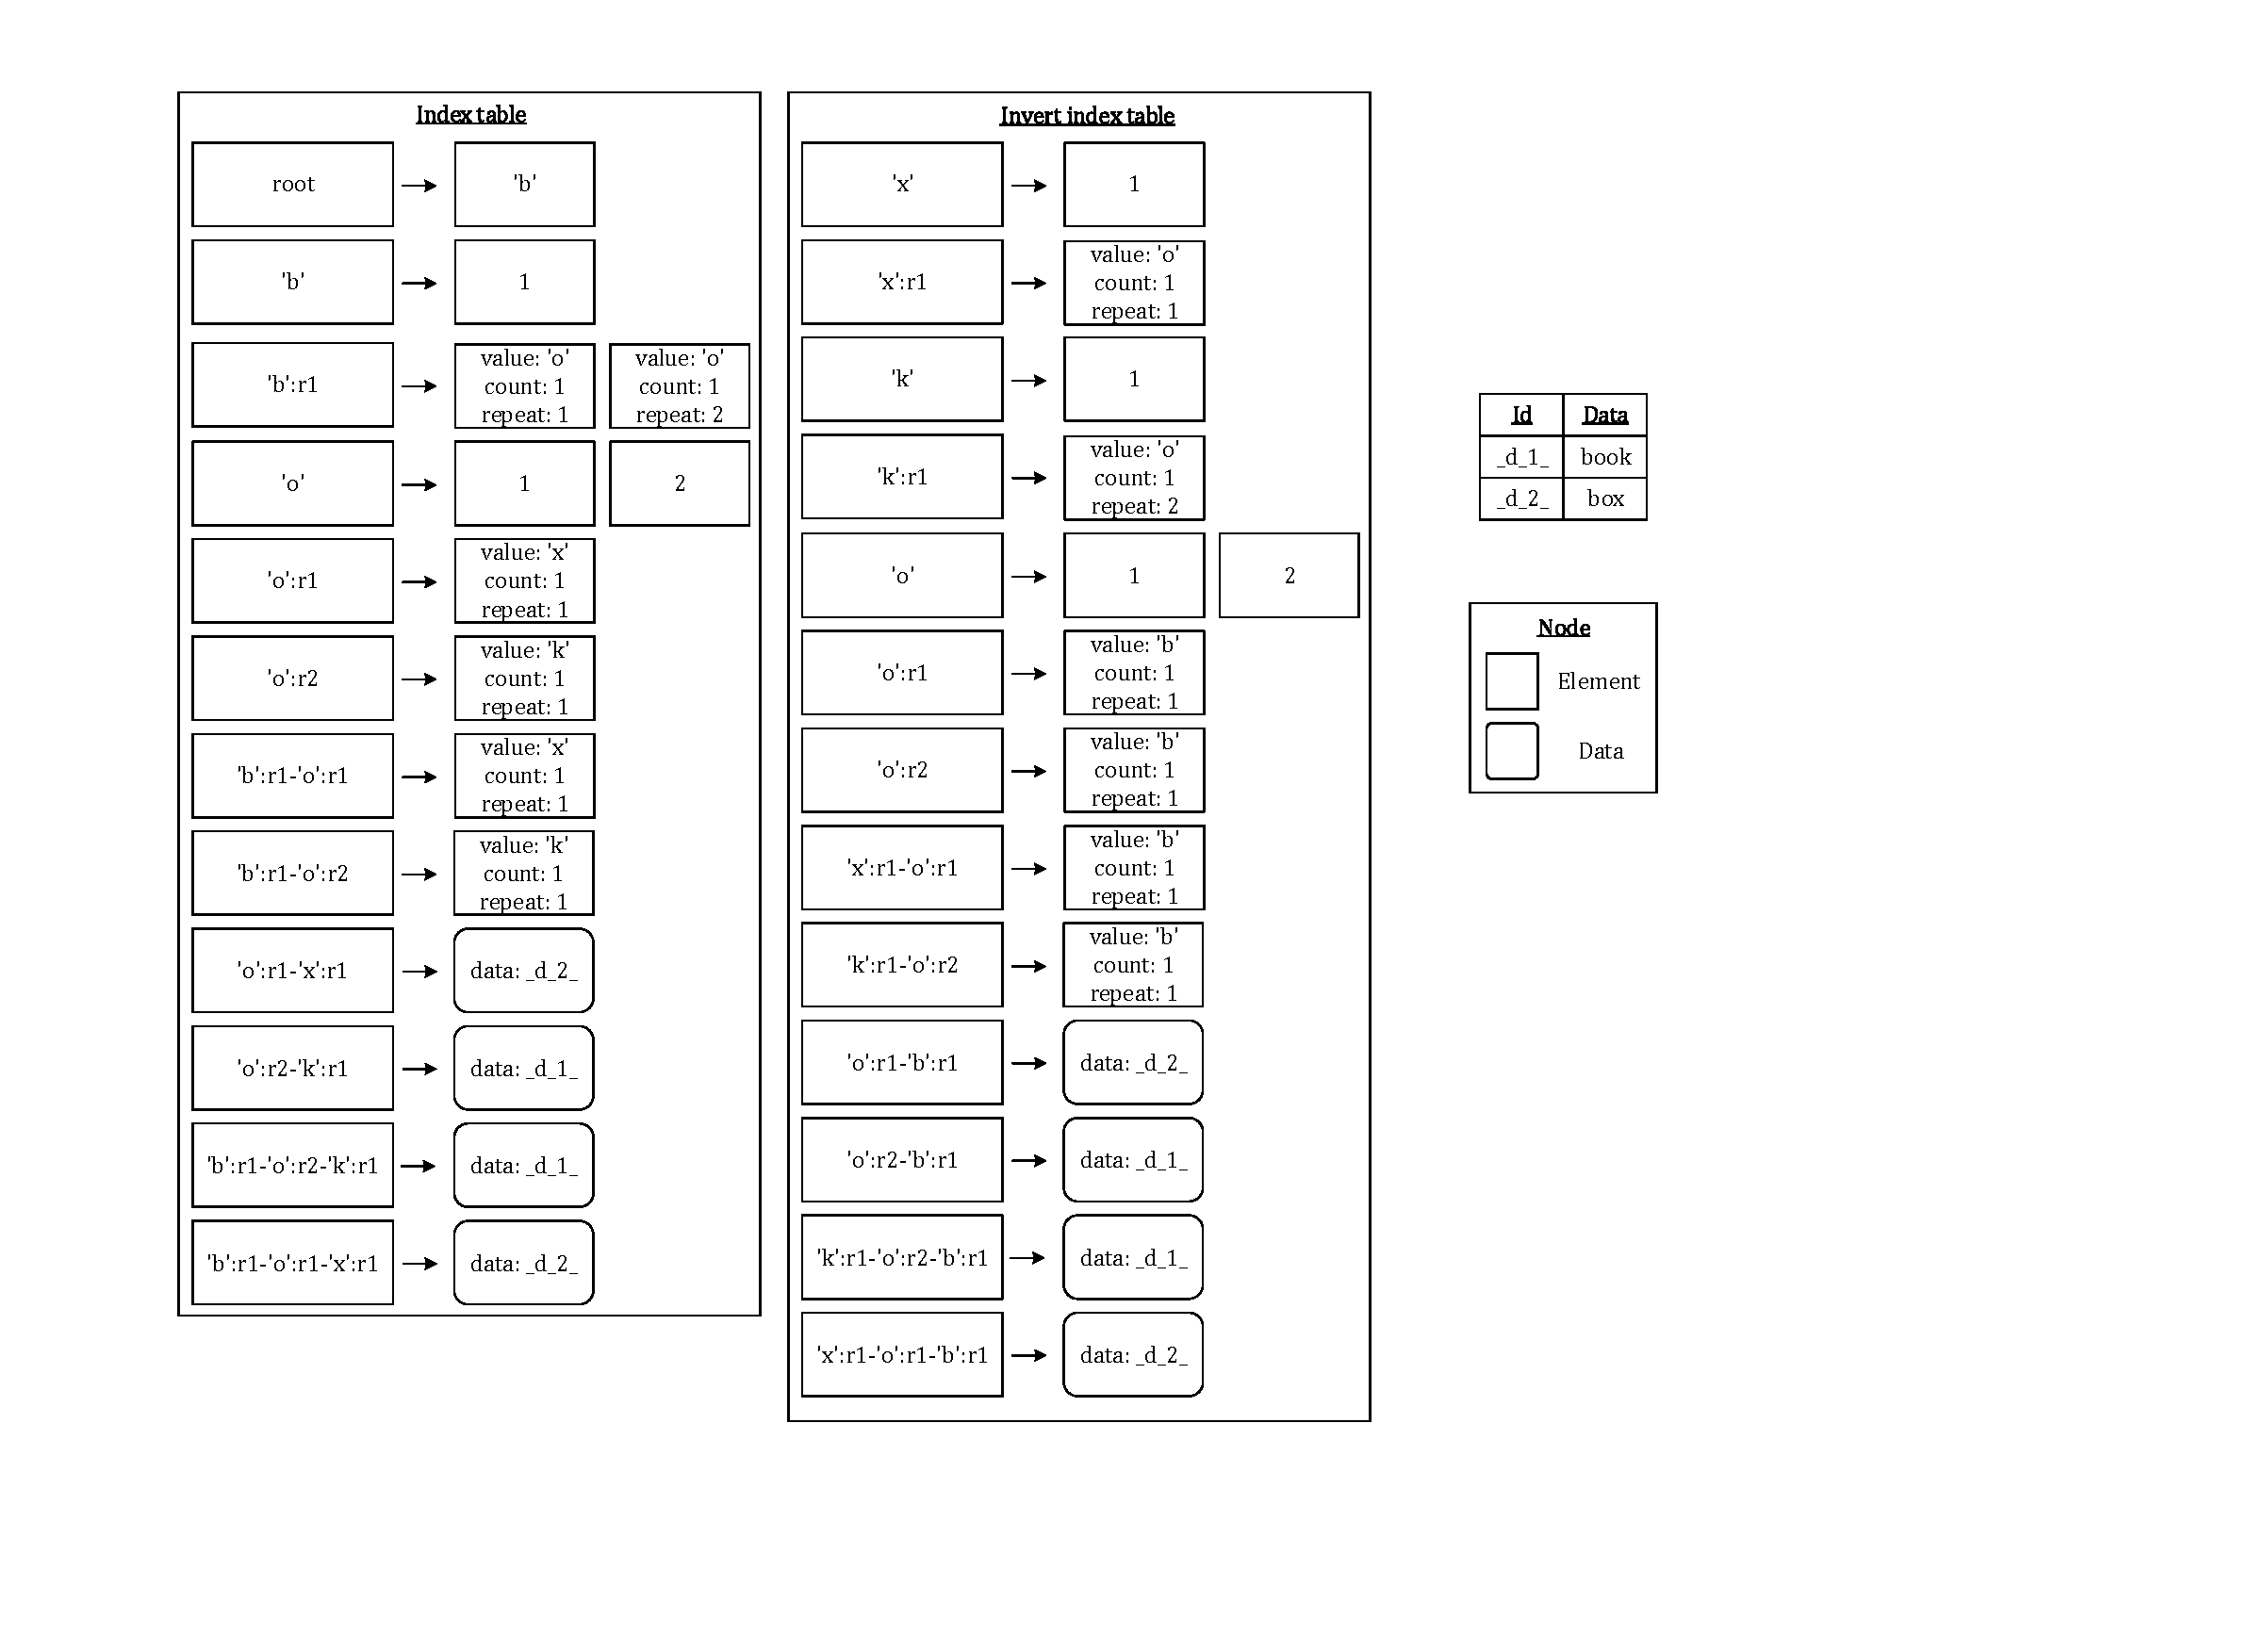
\includegraphics[scale=0.6]{./algorithm/string/pic/insertion/example_2_v5.pdf}
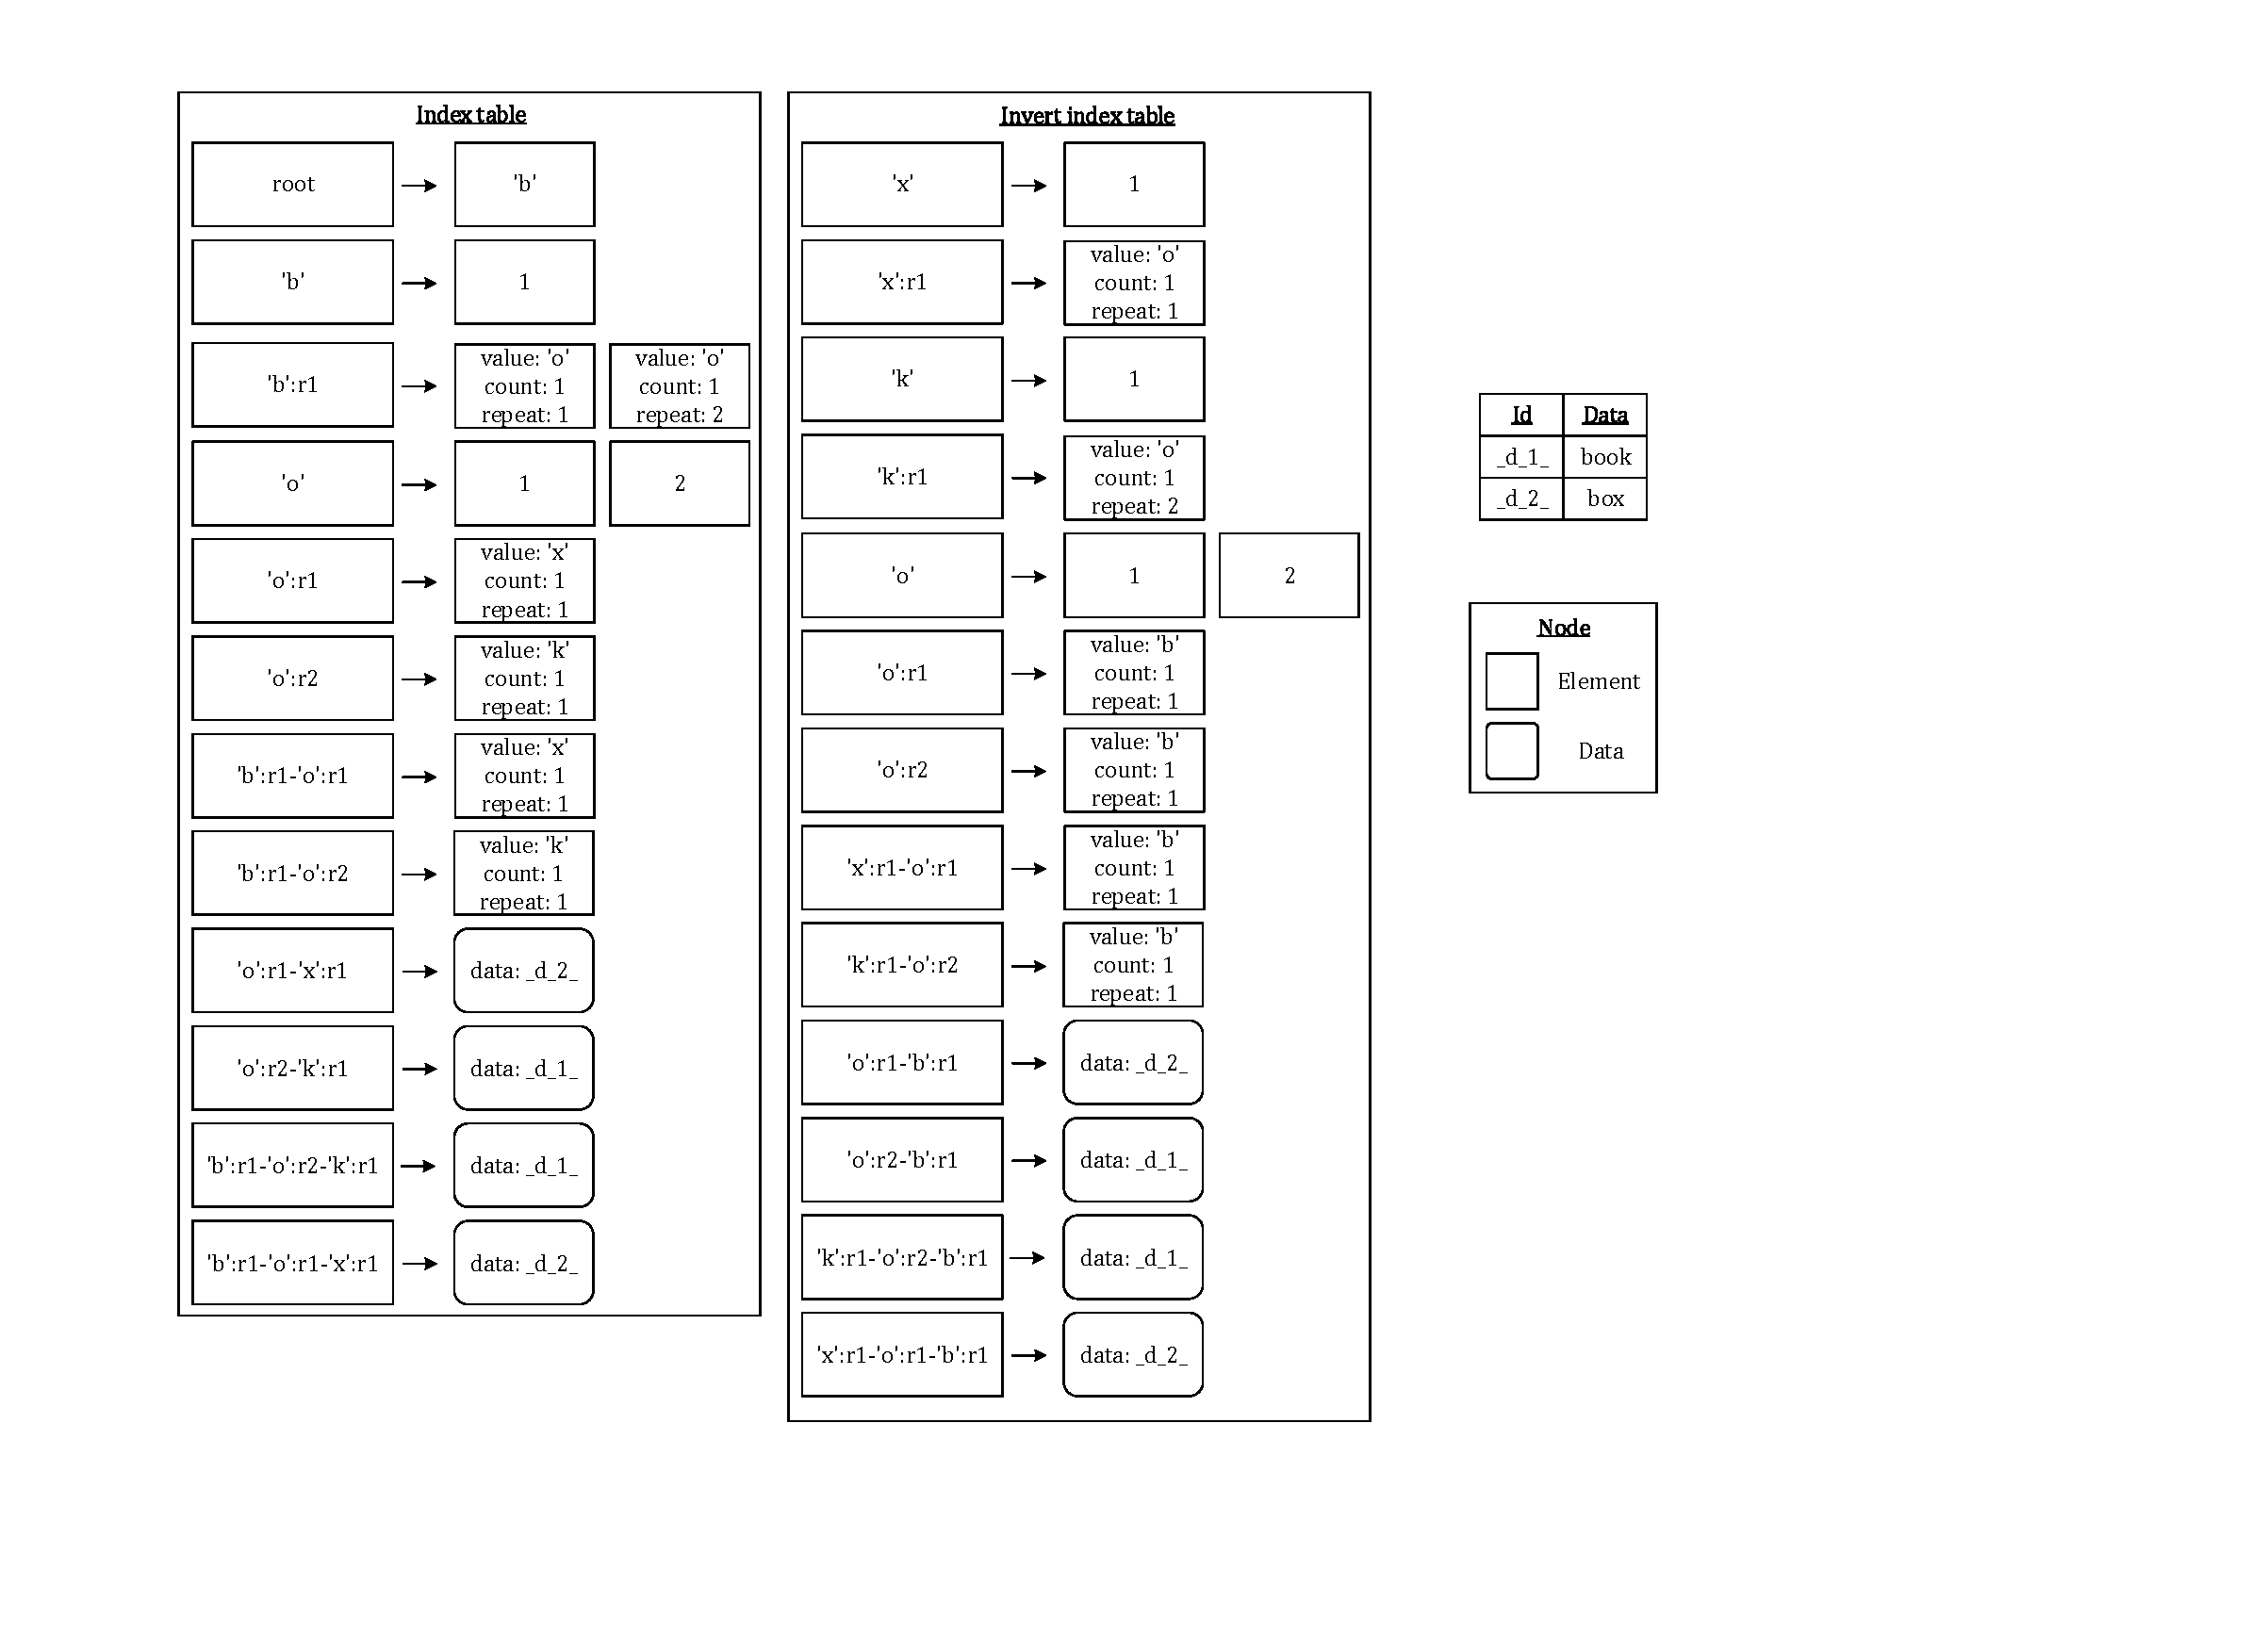
\includegraphics[width=0.8\textwidth]{./algorithm/string/pic/insertion/example_2_v5.pdf}
\caption{Insert data \textit{"box"}.}
\label{fig:algorithm:string:insertion:example_2}
\end{figure}



% Deletion section
\subsubsection{Deletion}

In deletion, if a data need to be delete, and the bucket is only contain one node or data, then this mapping will be delete, otherwise only the count in the node will minus one. Next, delete the n-gram indexing in all index table.\\

Using the same example in figure \ref{fig:algorithm:string:insertion:example_2}. If removing the $"book"$ which will remove some nodes in both index table, and then the tables should look like figure \ref{fig:algorithm:string:deletion:example_1}. For better understanding, the nodes which need to remove will use the line over it.

\begin{figure}[h]
\centering
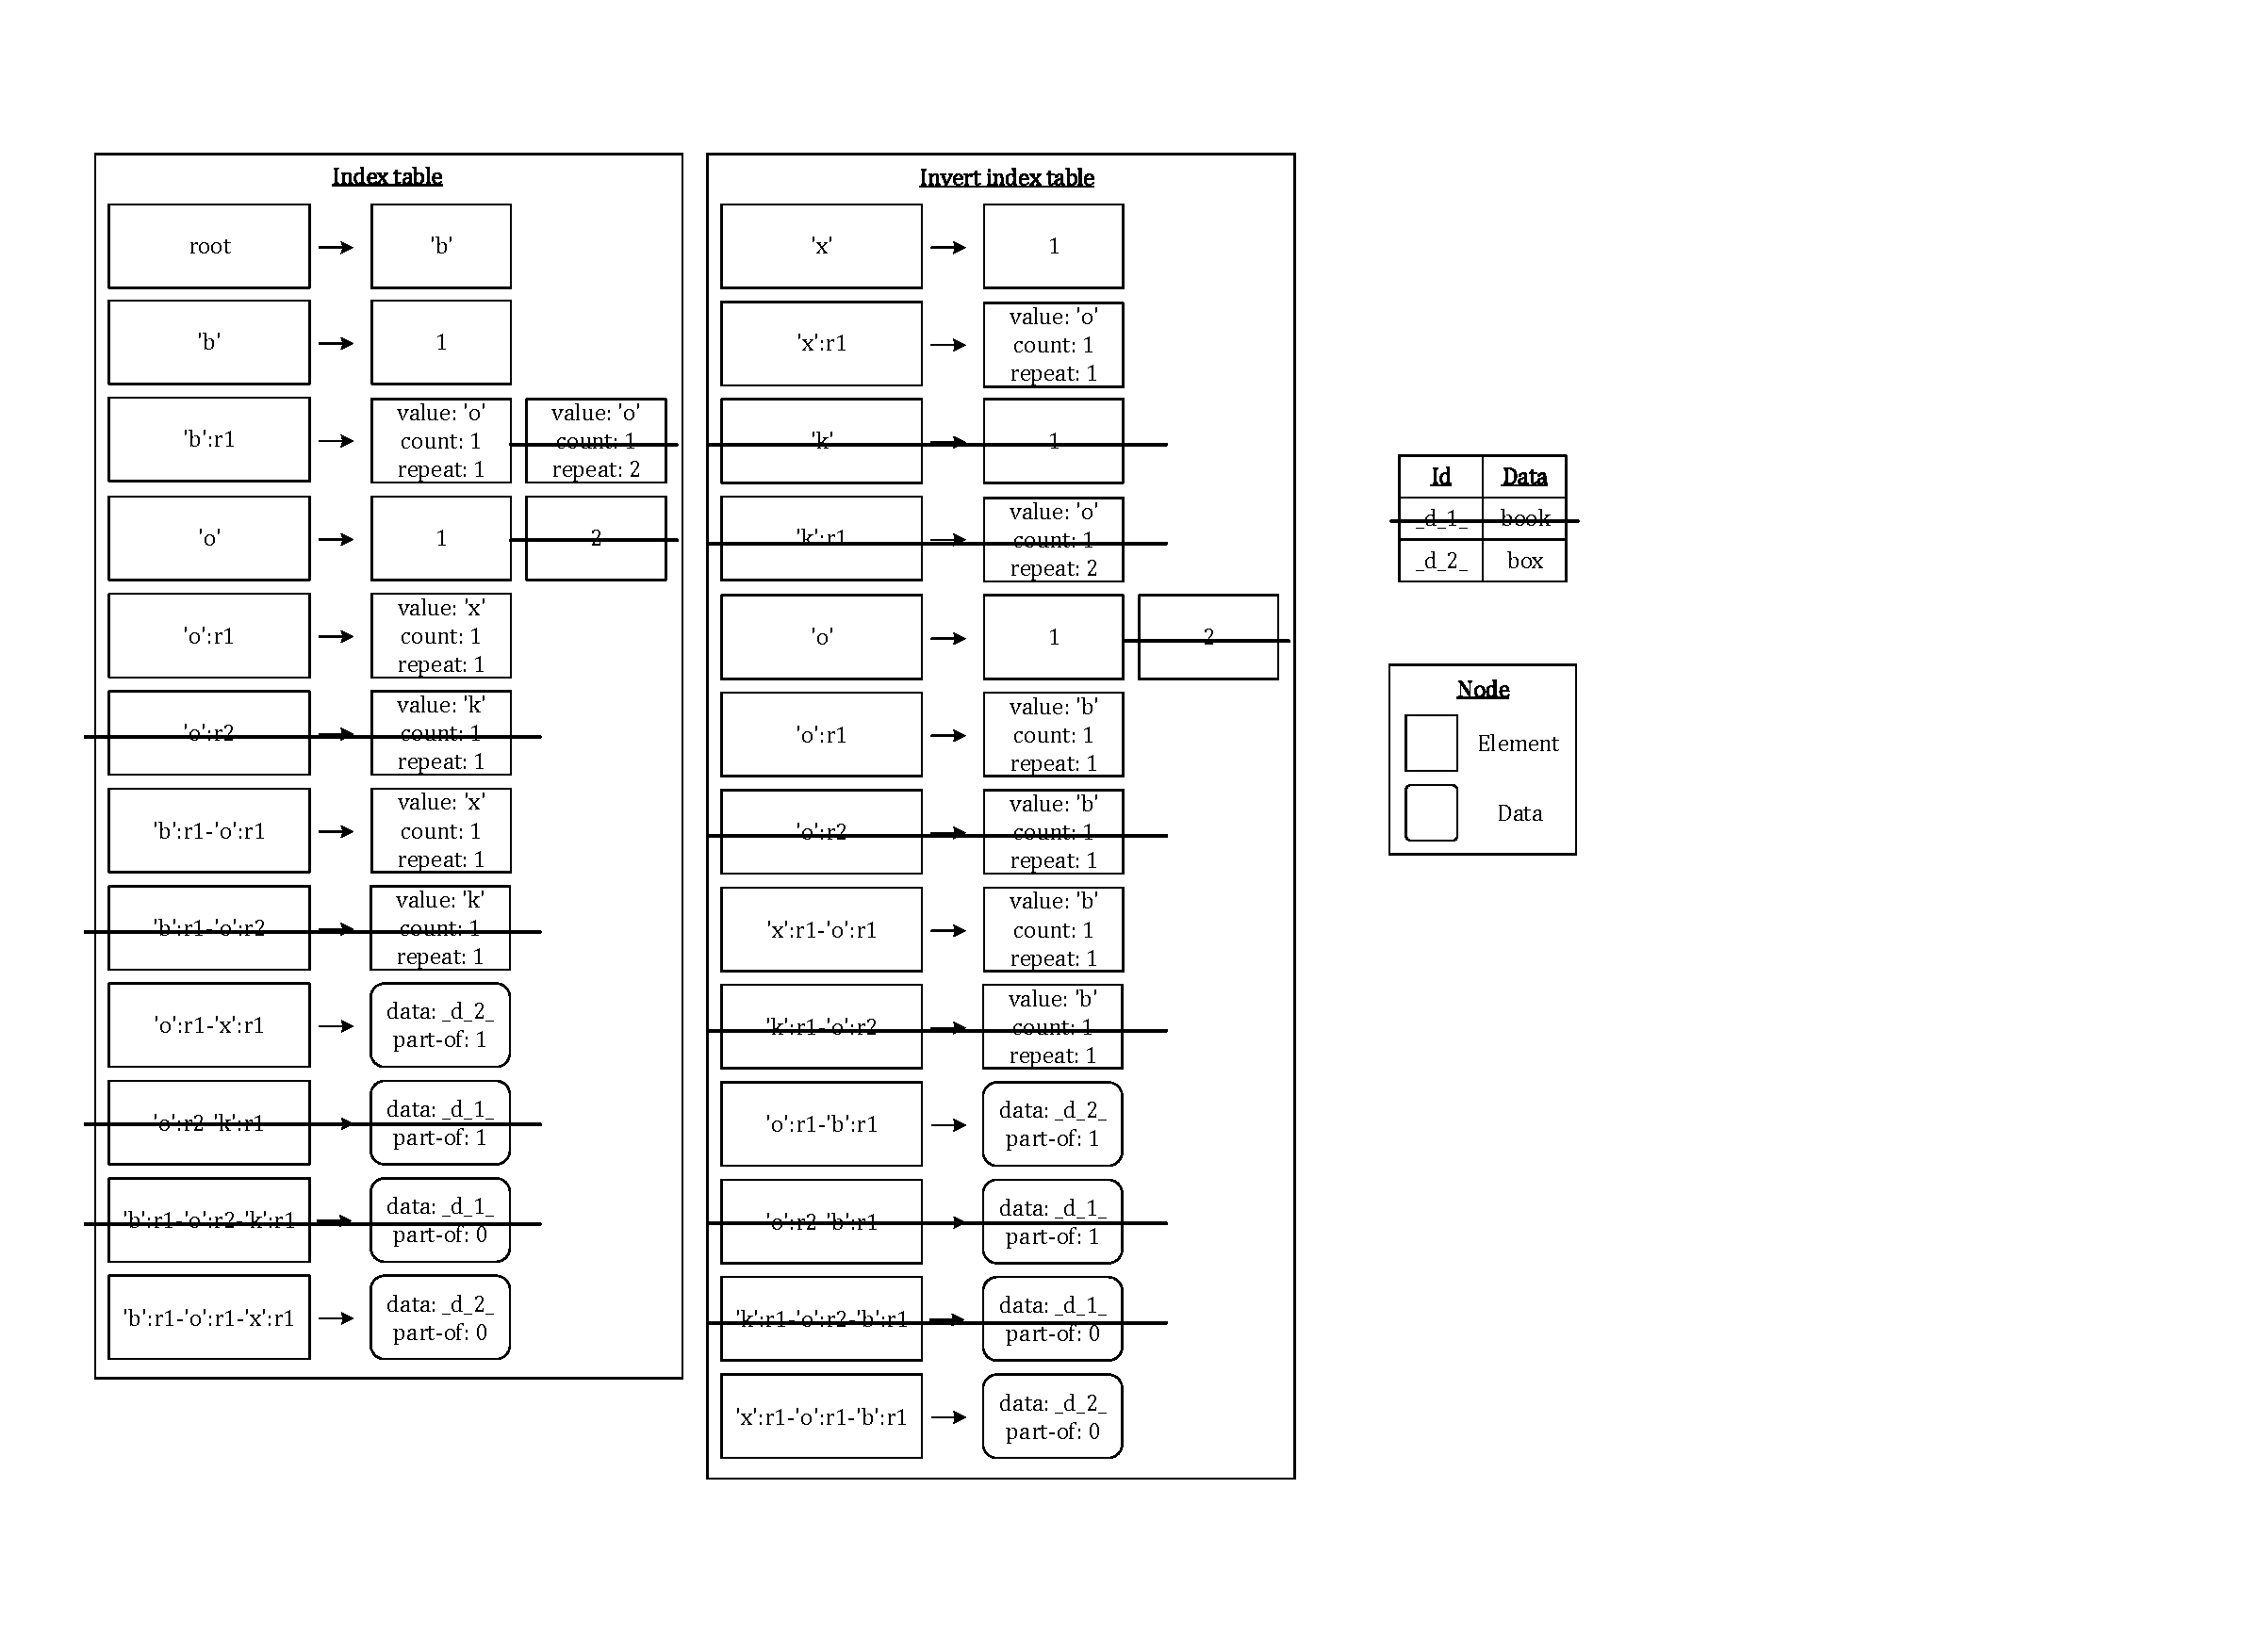
\includegraphics[scale=0.4]{./algorithm/string/pic/deletion/example_1_v3.pdf}
\caption{Delete $"book"$ from table.}
\label{fig:algorithm:string:deletion:example_1}
\end{figure}

The time needed is equals to $2 * O(b!)$, $b$ is the number of for loop which is equal to the byte length of string in one table (Normally it is equal, but in this case $(b = 3)$ which is because the $"o"$ have handled by the repeat counting). Because $2 * O(b!)$ is domain as $O(b)$, so the time complexity of delectation is $O(b)$.



% Modification section
\subsubsection{Modification}

Modify a data, actually is combining insert and delete, but without modified the data $id$. So the time complexity is $2 * O(b)$ operation but domain as $O(b)$.


% Selection section
\subsubsection{Selection}

The selection is the main core of Li's Hash, because the purposes of the index tables is to design for high-speed searching operation which means the Li's Hash can do the searching operation for key-value store.

Using the same example of figure \ref{fig:algorithm:string:insertion:example_2} from insertion section.

% Operation
\begin{enumerate}

% --------------------------------------------------------

\item \textbf{Exact matching}

As normal key-value store, if searching the data as \textit{"book"}, which convert into the key as \textit{"'b':r1-'o':r2-'k':r1"} and search in index table, and return the result of data node \textit{"\_d\_1\_"} in $O(1)$.

% --------------------------------------------------------

\item \textbf{Prefix matching}

If searching \textit{"bo"} as prefix which as same as \textit{"LIKE 'bo\%'"} in SQL. Using the key as \textit{"'b':r1"} from index table, will get the metadata that can know the next keys \textit{"'b':r1$-$'o':r1"} and \textit{"'b':r1$-$'o':r2"}. So fellow these two keys will get \textit{"'b':r1-'o':r1-'x':r1"} and \textit{"'b':r1-'o':r2-'k':r1"}, and using this two keys will get the data node \textit{"\_d\_1\_"} and \textit{"\_d\_2\_"}.

So the concept of search is fellow the metadata if get an element node, and add the data into the return list if pointing to a data node. Repeat search in table with this way until there is no element node can fellow.

And the time complexity should be $O(b)$.

% --------------------------------------------------------

\item \textbf{Suffix matching}

Similar as prefix matching, the different is using inverted index table rather than index table. So if try to search \textit{'x'} as suffix which as same as \textit{"LIKE '\%x'"} in SQL, using the key \textit{'x'} and get \textit{"'x':r1"} as return, and the remain is as same as the searching in prefix matching which will get the data node \textit{"\_d\_2\_"} in final. The time complexity is $O(b)$.

% --------------------------------------------------------

\item \textbf{Partial matching}

Partial matching is combining the prefix and suffix matching. For example if search \textit{'o'} for result which as same as using \textit{"LIKE '\%o\%'"} in SQL, then reassign as \textit{'o'} for prefix matching (\textit{"LIKE 'o\%'"} in SQL) and suffix matching (\textit{"LIKE '\%o'"} in SQL), and the last step is to do intersection to both result.

The reason of existing the special keys is to record the repeat time like\textit{'o'-\textgreater1} or \textit{2}, or some keys like \textit{"'o':r1}-\textit{'x':r1"} which are target on this operation.

If these keys are not created, the search like above wouldn't be searchable because the \textit{'o'} is middle of the keys, it can't be found unless there is some query function provided by non-relational database where are  range scan or full scan, but we have already mentioned before.

And the time complexity should be $O(b) + O(b)$ that domain as $O(b)$.

% --------------------------------------------------------

\item \textbf{Retrieve all}

Using the key of \textit{"root"} in index table will get all the prefix byte of all result, this can simple retrieve all data in the database which the time complexity be $O(b)$.

% --------------------------------------------------------

\end{enumerate}


% Summary section
\subsubsection{Summary}

Table \ref{table:algorithm:string:summary:time_complexity} is the summary the time complexity of each opration in \textit{STRING} type.

\begin{table}[h]
\centering
\caption{Time complexity for \textit{STRING} type.}
\label{table:algorithm:string:summary:time_complexity}
\begin{tabular}{|c|c|}

\hline
\multicolumn{1}{|c|}{Operation} &
\multicolumn{1}{c|}{\tabincell{c}{
Time complexity \\ ($b$: The byte length of data)
}} \\

\hline
\multicolumn{1}{|c|}{Insert} &
\multicolumn{1}{c|}{$O(b)$} \\

\hline
\multicolumn{1}{|c|}{Modify} &
\multicolumn{1}{c|}{$O(b)$} \\

\hline
\multicolumn{1}{|c|}{Delete} &
\multicolumn{1}{c|}{$O(b)$} \\

\hline
\multicolumn{1}{|c|}{\tabincell{c}{
Search \\ (Exact matching)
}} &
\multicolumn{1}{c|}{$O(1)$} \\

\hline
\multicolumn{1}{|c|}{\tabincell{c}{
Search \\ (Prefix matching)
}} &
\multicolumn{1}{c|}{$O(b)$} \\

\hline
\multicolumn{1}{|c|}{\tabincell{c}{
Search \\ (Suffix matching)
}} &
\multicolumn{1}{c|}{$O(b)$} \\

\hline
\multicolumn{1}{|c|}{\tabincell{c}{
Search \\ (Partial matching)
}} &
\multicolumn{1}{c|}{$O(b)$} \\

\hline
\multicolumn{1}{|c|}
{\tabincell{c}{
Search \\ (Retrieve all)
}} &
\multicolumn{1}{c|}
{\tabincell{c}{
$O(b)$ \\ ($b$ is the longest string of all data)
}} \\

\hline
\end{tabular}
\end{table}


\clearpage


% BOOLEAN section
\subsection{BOOLEAN type}

The indexing in \textit{BOOLEAN} type is the simplest than other type, the invert index table is not needed because it is useless by doing the invert indexing just one single byte. So the table can be simplify as figure \ref{fig:algorithm:boolean:example_1}.

\begin{figure}[ht]
\centering
%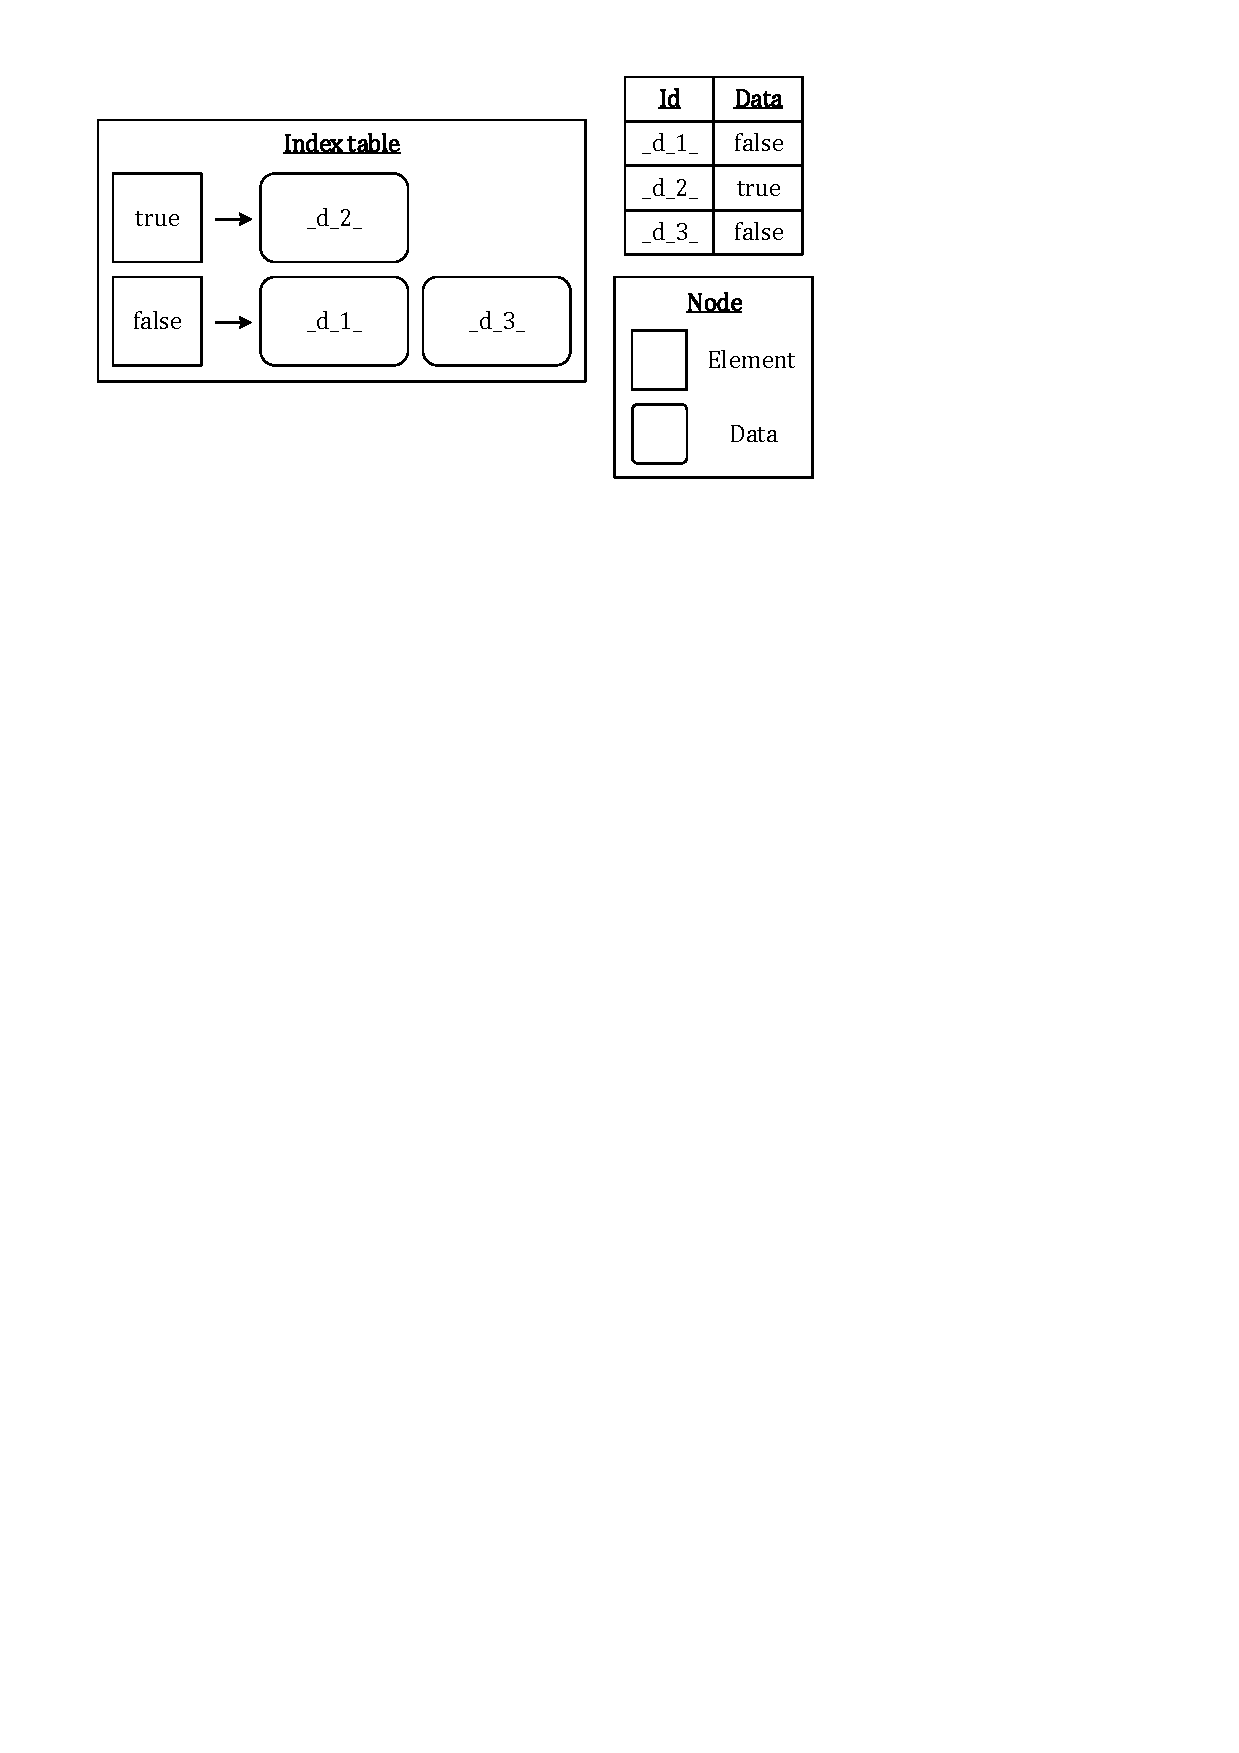
\includegraphics[scale=0.8]{./algorithm/boolean/pic/example_1_v1.pdf}
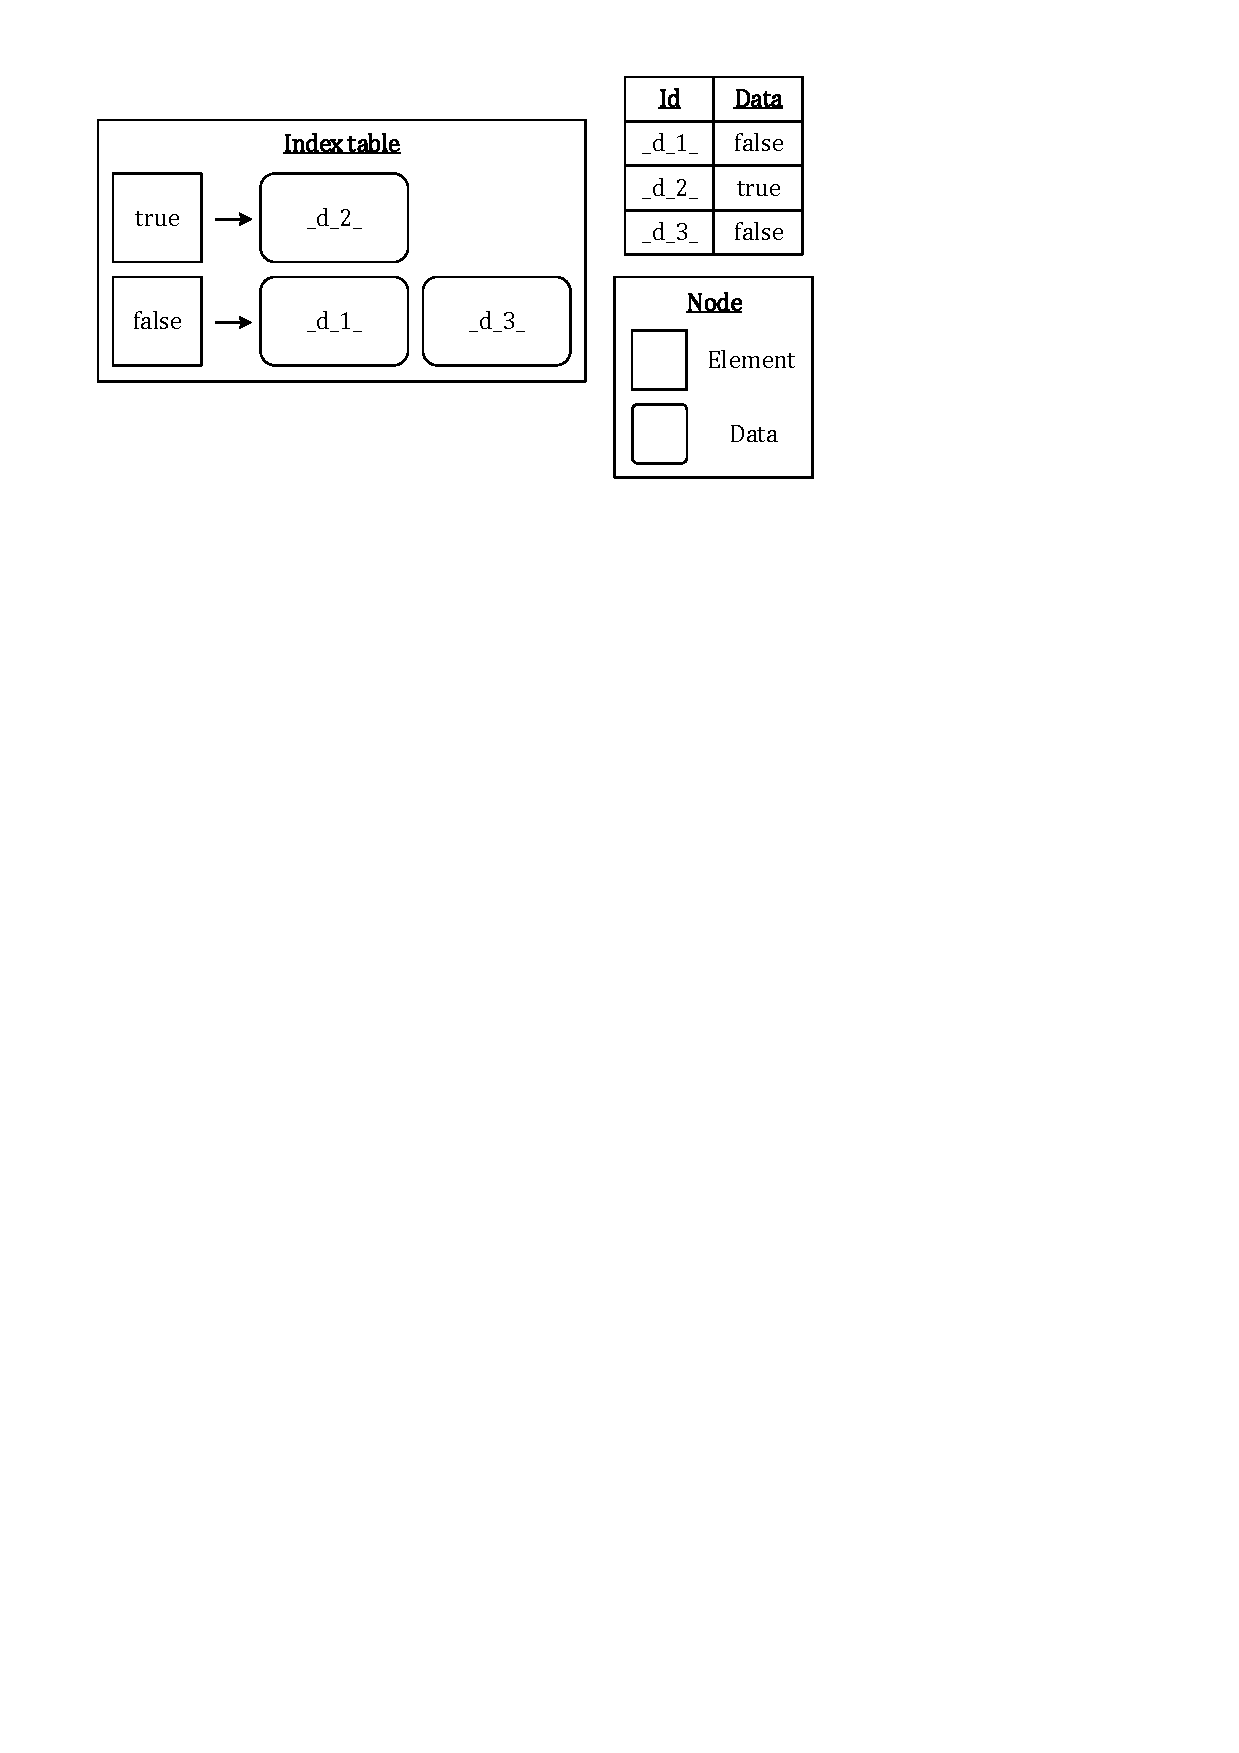
\includegraphics[width=0.8\textwidth]{./algorithm/boolean/pic/example_1_v1.pdf}
\caption{The indexing tables of in \textit{BOOLEAN} type.}
\label{fig:algorithm:boolean:example_1}
\end{figure}


% Insertion section
\subsubsection{Insertion}

When inserting a new data, it just need to add the data node into the bucket where the data belong with, so the time complexity should be $O(1)$.


% Deletion section
\subsubsection{Deletion}

Delete a data node is just get the bucket and remove the data node, so this is also a quick operation where time complexity be $O(1)$.


% Modification section
\subsubsection{Modification}

Modify the data is actually delete the node in a bucket and re-insert it again into another bucket. Time complexity should be $O(1)$.



% Selection section
\subsubsection{Selection}

Select operation is the simplest operation than the other, because the selection for \textit{BOOLEAN} type is only can select $"true"$ or $"false"$, so select the bucket then this will return the whole bucket, so this is also a quick operation. Also if user want to retrieve all, just retrieve both $"true"$ and $"false"$ bucket will get all data. That time complexity of both searching are $O(1)$.


% Summary section
\subsubsection{Summary}

Table \ref{table:algorithm:boolean:summary:time_complexity} is summarized the time complexity of each opration in \textit{BOOLEAN} type.

\begin{table}[h]
\centering
\caption{Time complexity for \textit{BOOLEAN} type.}
\label{table:algorithm:boolean:summary:time_complexity}
\begin{tabular}{|c|c|}

\hline
\multicolumn{1}{|c|}{Operation} &
\multicolumn{1}{c|}{Time complexity} \\

\hline
\multicolumn{1}{|c|}{Insert} &
\multicolumn{1}{c|}{$O(1)$} \\

\hline
\multicolumn{1}{|c|}{Modify} &
\multicolumn{1}{c|}{$O(1)$} \\

\hline
\multicolumn{1}{|c|}{Delete} &
\multicolumn{1}{c|}{$O(1)$} \\

\hline
\multicolumn{1}{|c|}{Selection} &
\multicolumn{1}{c|}{$O(1)$} \\

\hline
\end{tabular}
\end{table}


\clearpage


% INTEGER section
\subsection{INTEGER type}

The \textit{INTEGER} type is design as 8 bytes $({b} = 8)$, but for easy to explain the \textit{INTEGER} type design in Li's Hash, so the example below which will explain in 4 bytes $(b = 4)$.\\

As normal integer, the \textit{INTEGER} type can be also signed and unsigned, this information will record in the metadata, so this will not show in index table, the different between them is the operation have a little bit different, but they share the same index table. Same as the \textit{BOOLEAN} type, the invert index table is not needed. Because of the inverted index table cost spaces but don't provide a significant speed up for the operation.\\

We use figure \ref{fig:algorithm:integer:example_1} to explain these operations below:

\begin{figure}[h]
\centering
%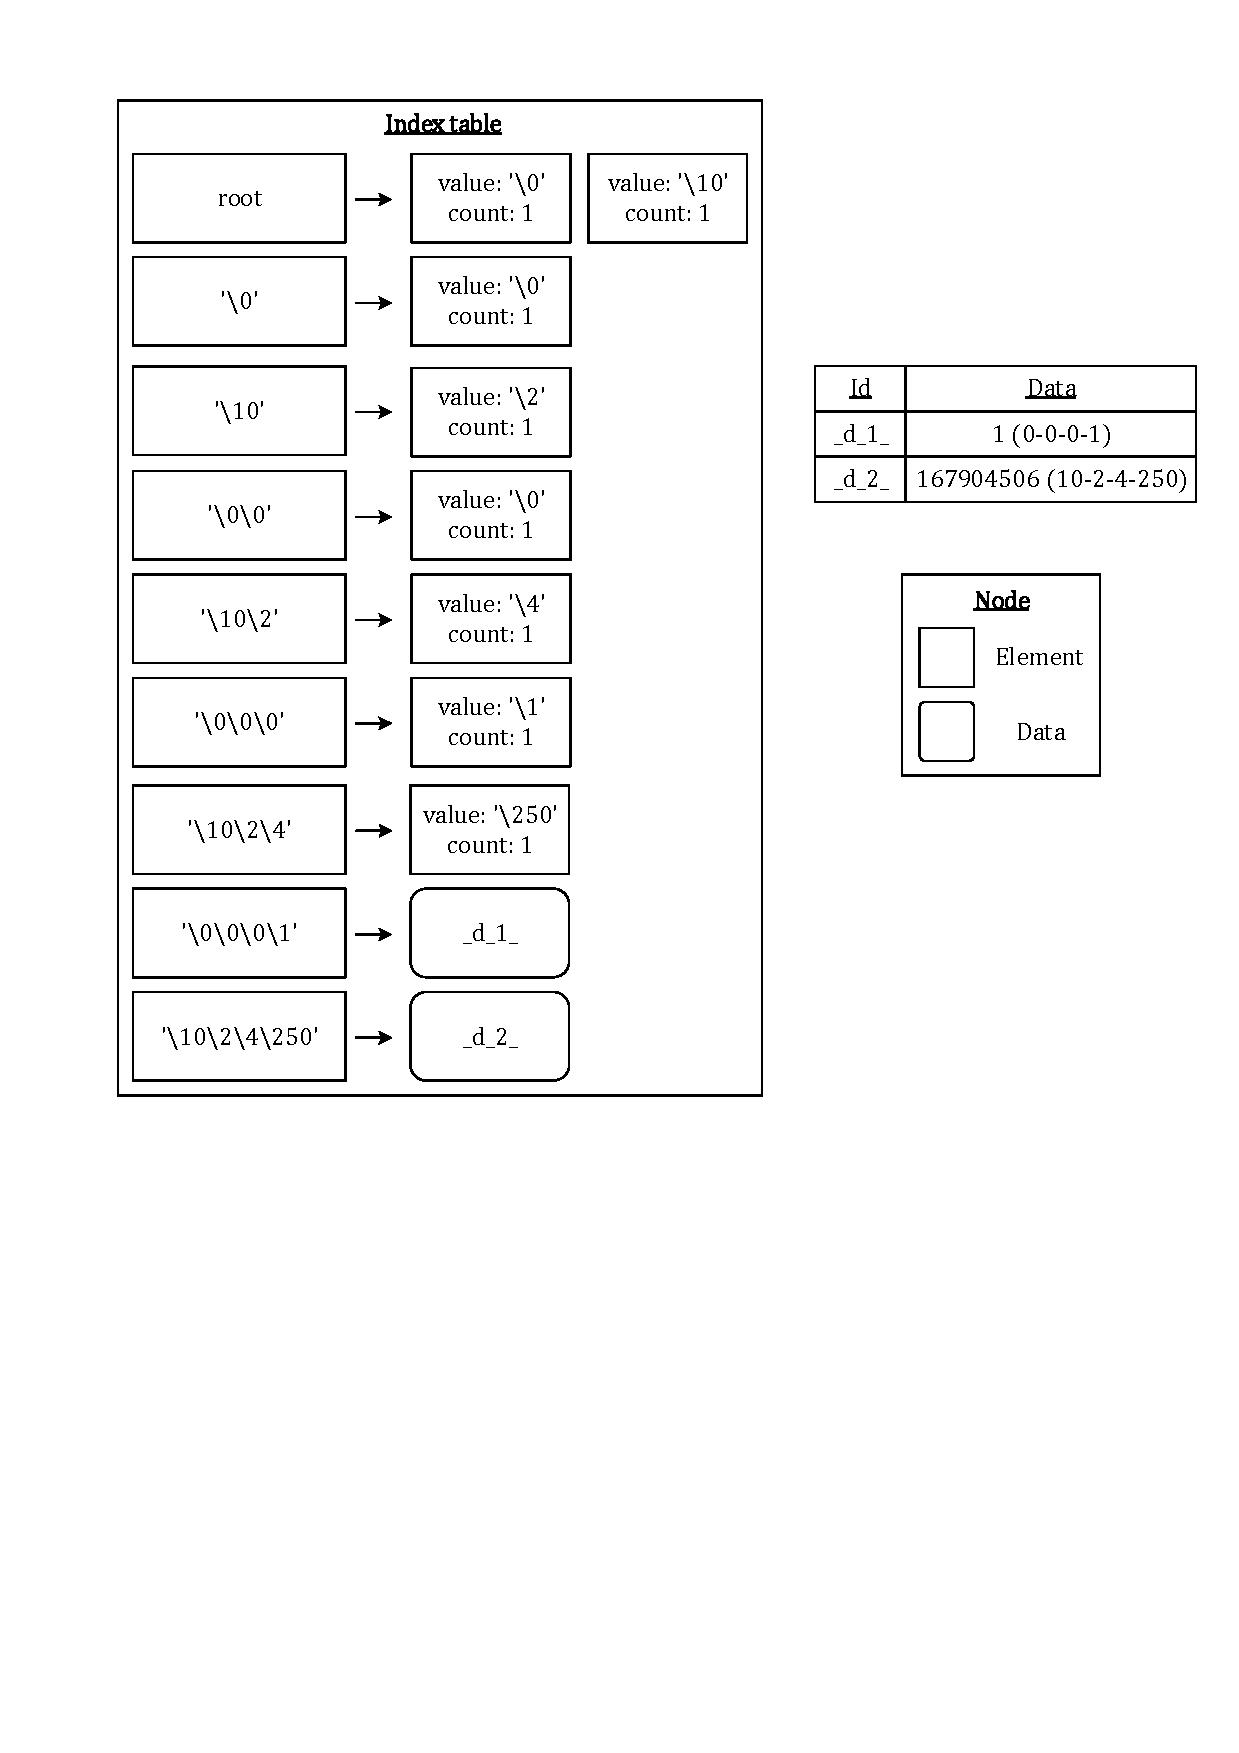
\includegraphics[scale=0.45]{./algorithm/integer/pic/example_1_v3.pdf}
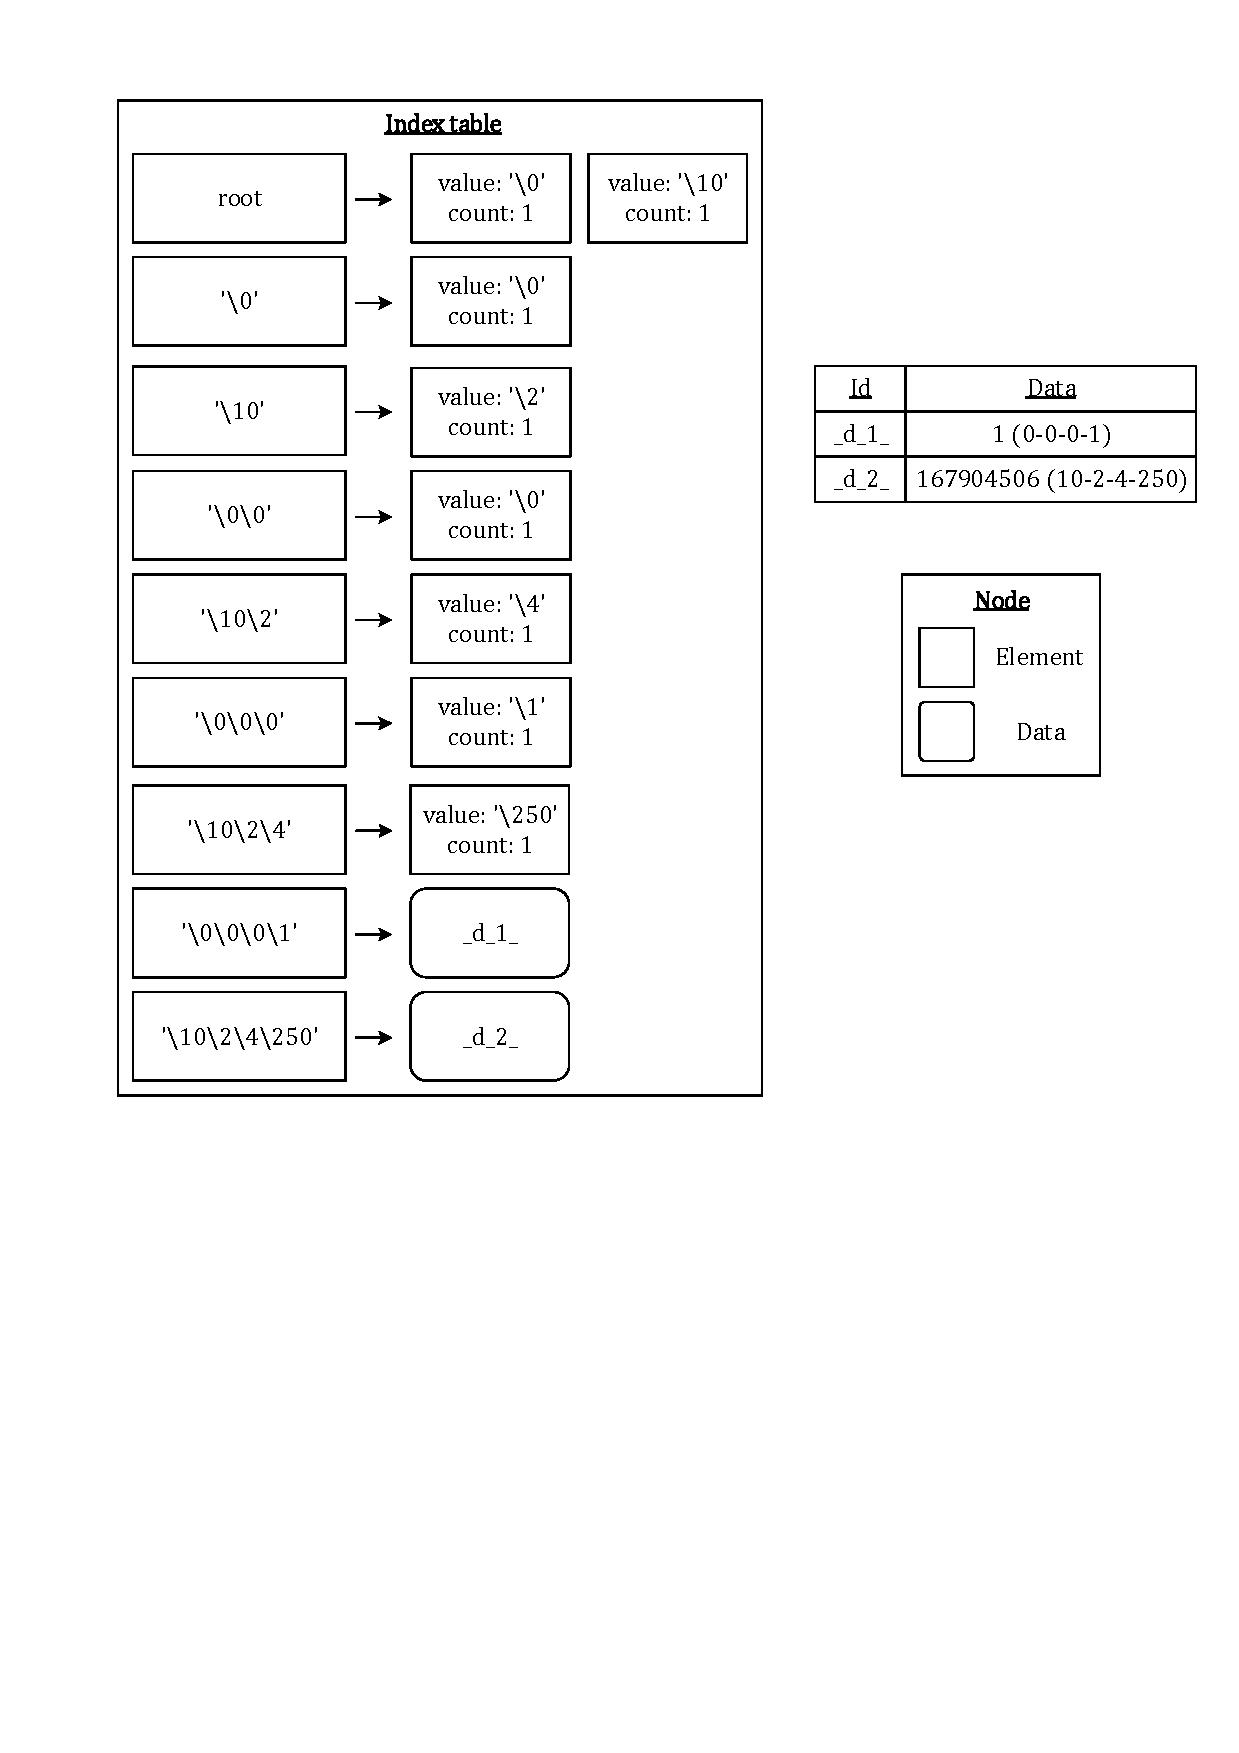
\includegraphics[width=0.8\textwidth]{./algorithm/integer/pic/example_1_v3.pdf}
\caption{The indexing tables of \textit{INTEGER} type.}
\label{fig:algorithm:integer:example_1}
\end{figure}

The index table is start with a root key \textit{'root'}. The root key is use to record the first byte of the data, so it will point to the range of 0 to 255.\\

In figure \ref{fig:algorithm:integer:example_1}, there are two data in the table. The four bytes of \textit{1} is \textit{0-0-0-1}, and \textit{167904506} is \textit{10-2-4-250} in byte. So in the table, the \textit{'root'} is pointing to \textit{'$\backslash0$'} and \textit{'$\backslash10$'}. After root key is finish its' indexing, the next step is just using n-gram indexing to index remain bytes to store data in the table.\\


% Insertion section
\subsubsection{Insertion}

Figure \ref{fig:algorithm:integer:example_1} already described some of the flow of insertion, so in here will show the table if insert a negative value into the table. Insert a -2147483647 (128-0-0-1) into table, which will become like figure \ref{fig:algorithm:integer:insertion:example_1}.

\begin{figure}[h]
\centering
%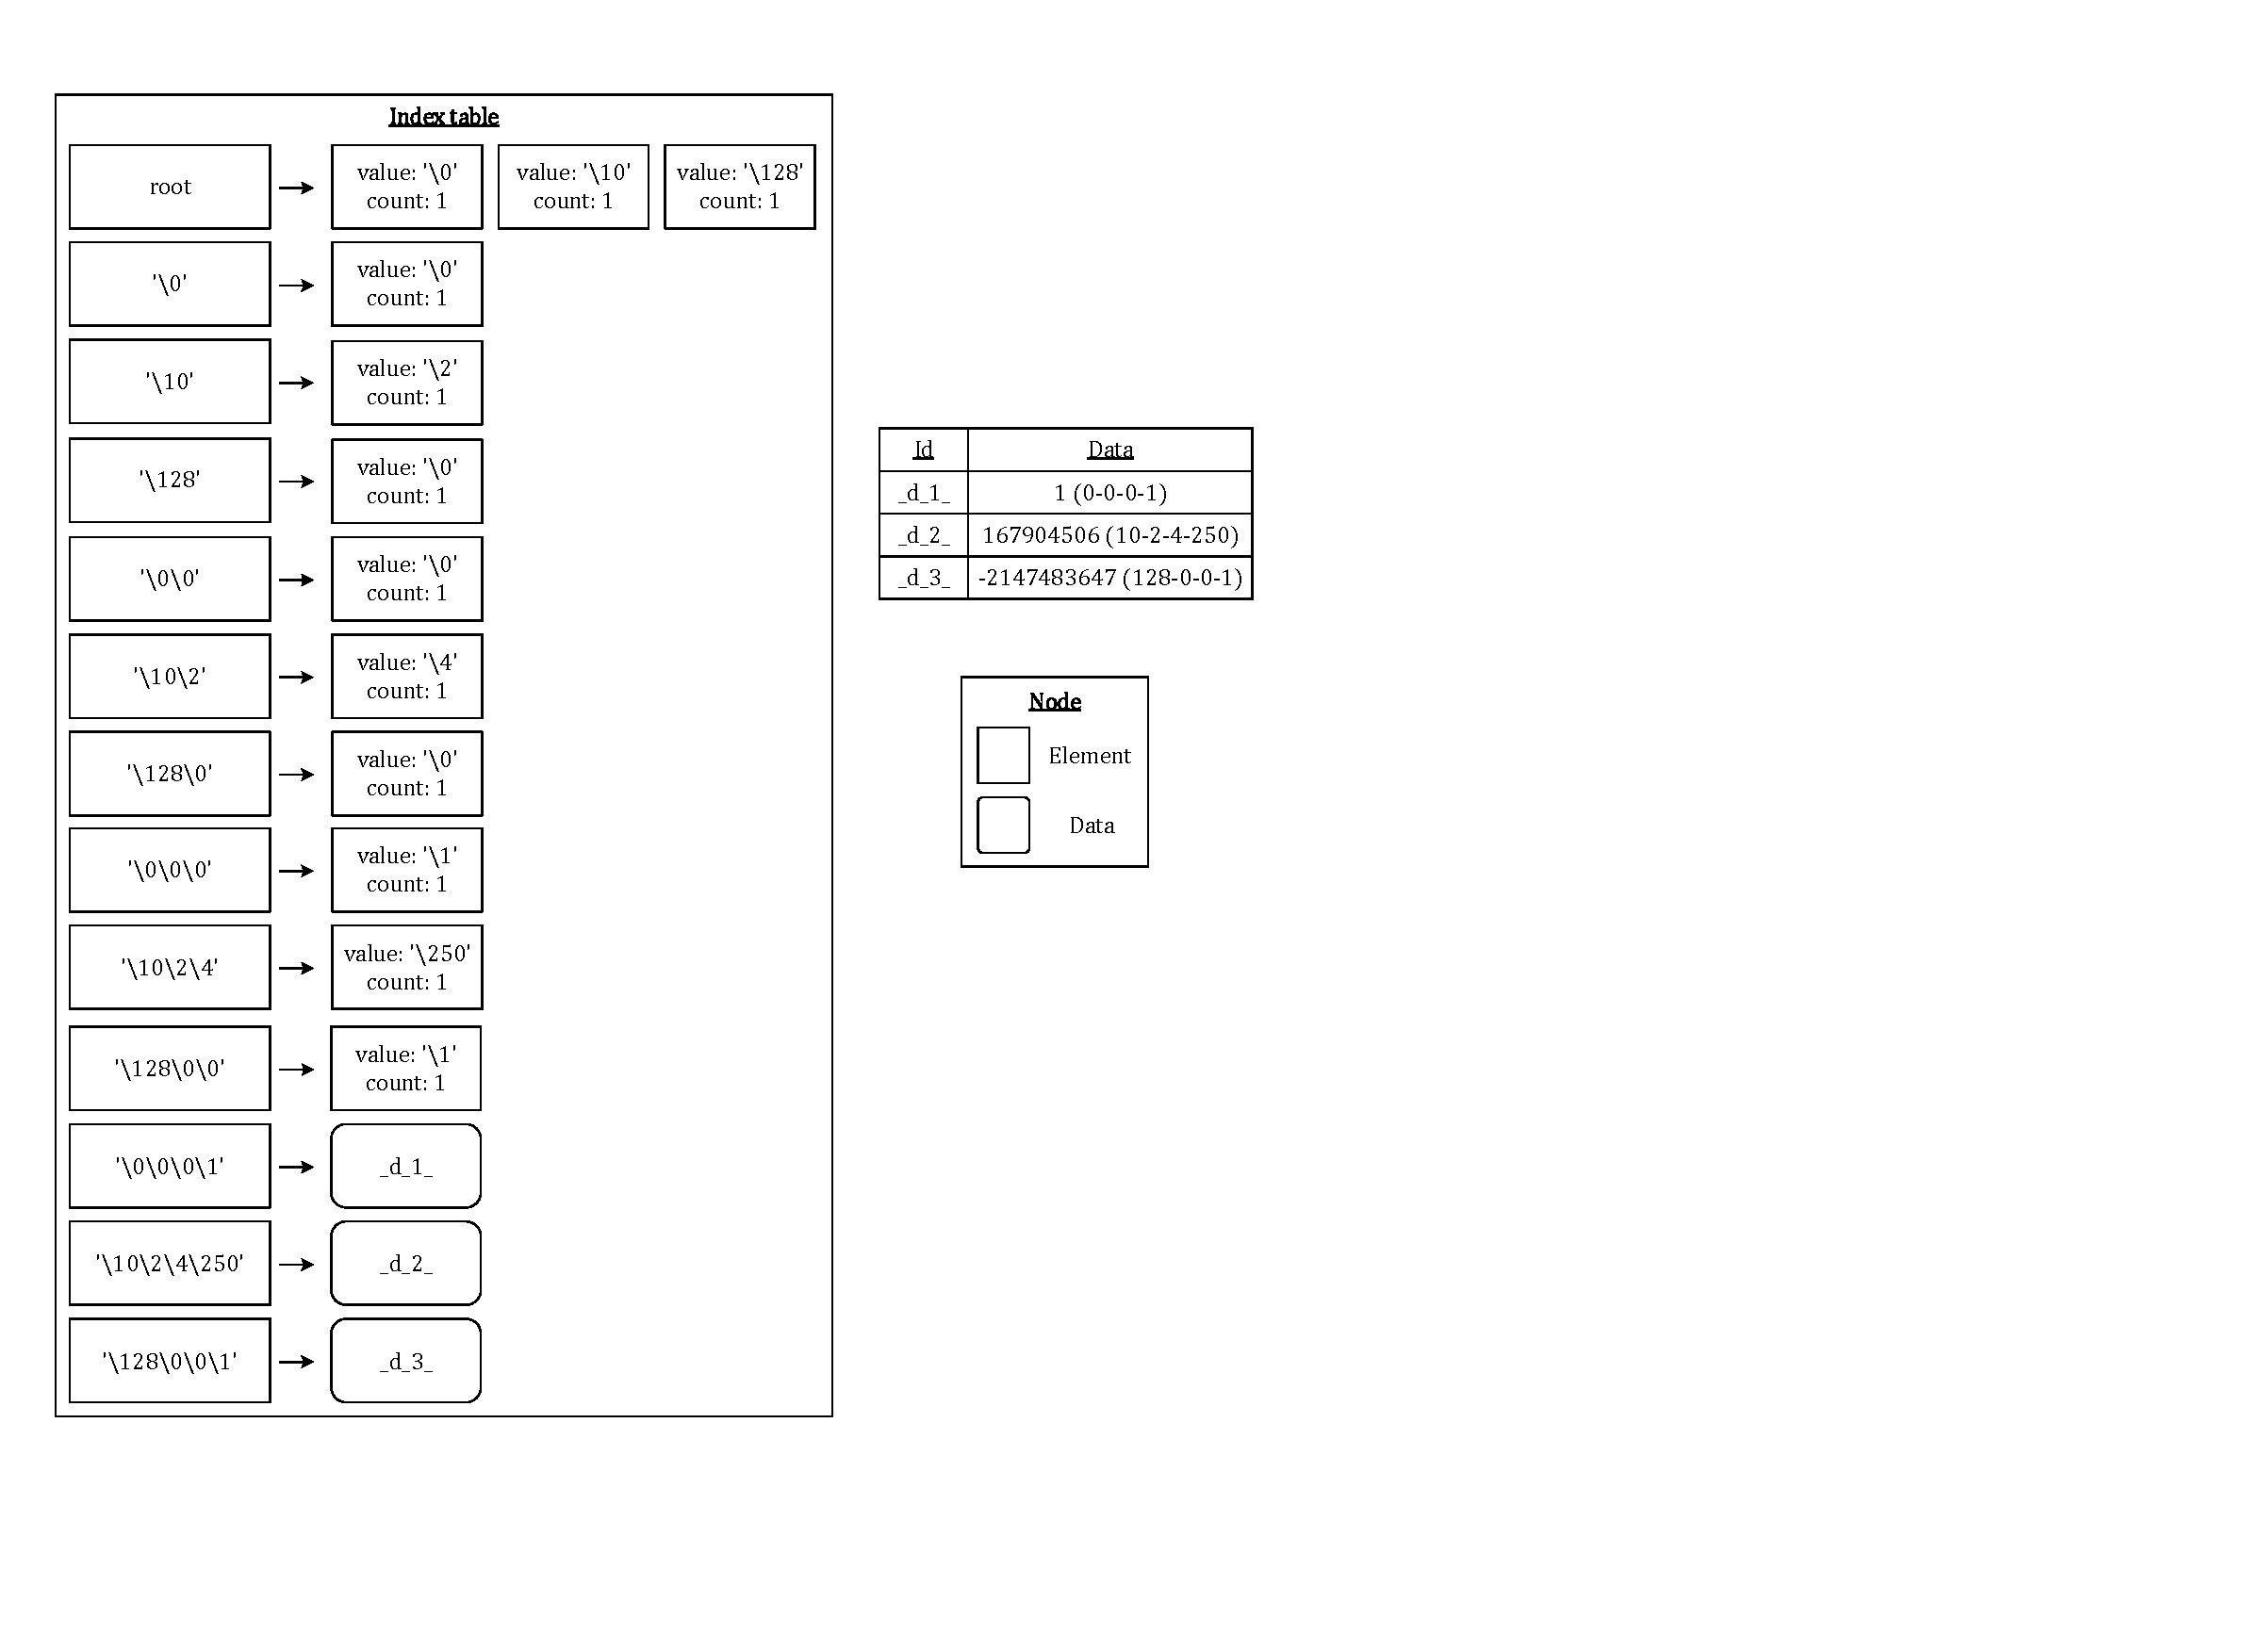
\includegraphics[scale=0.6]{./algorithm/integer/pic/insertion/example_1_v3.pdf}
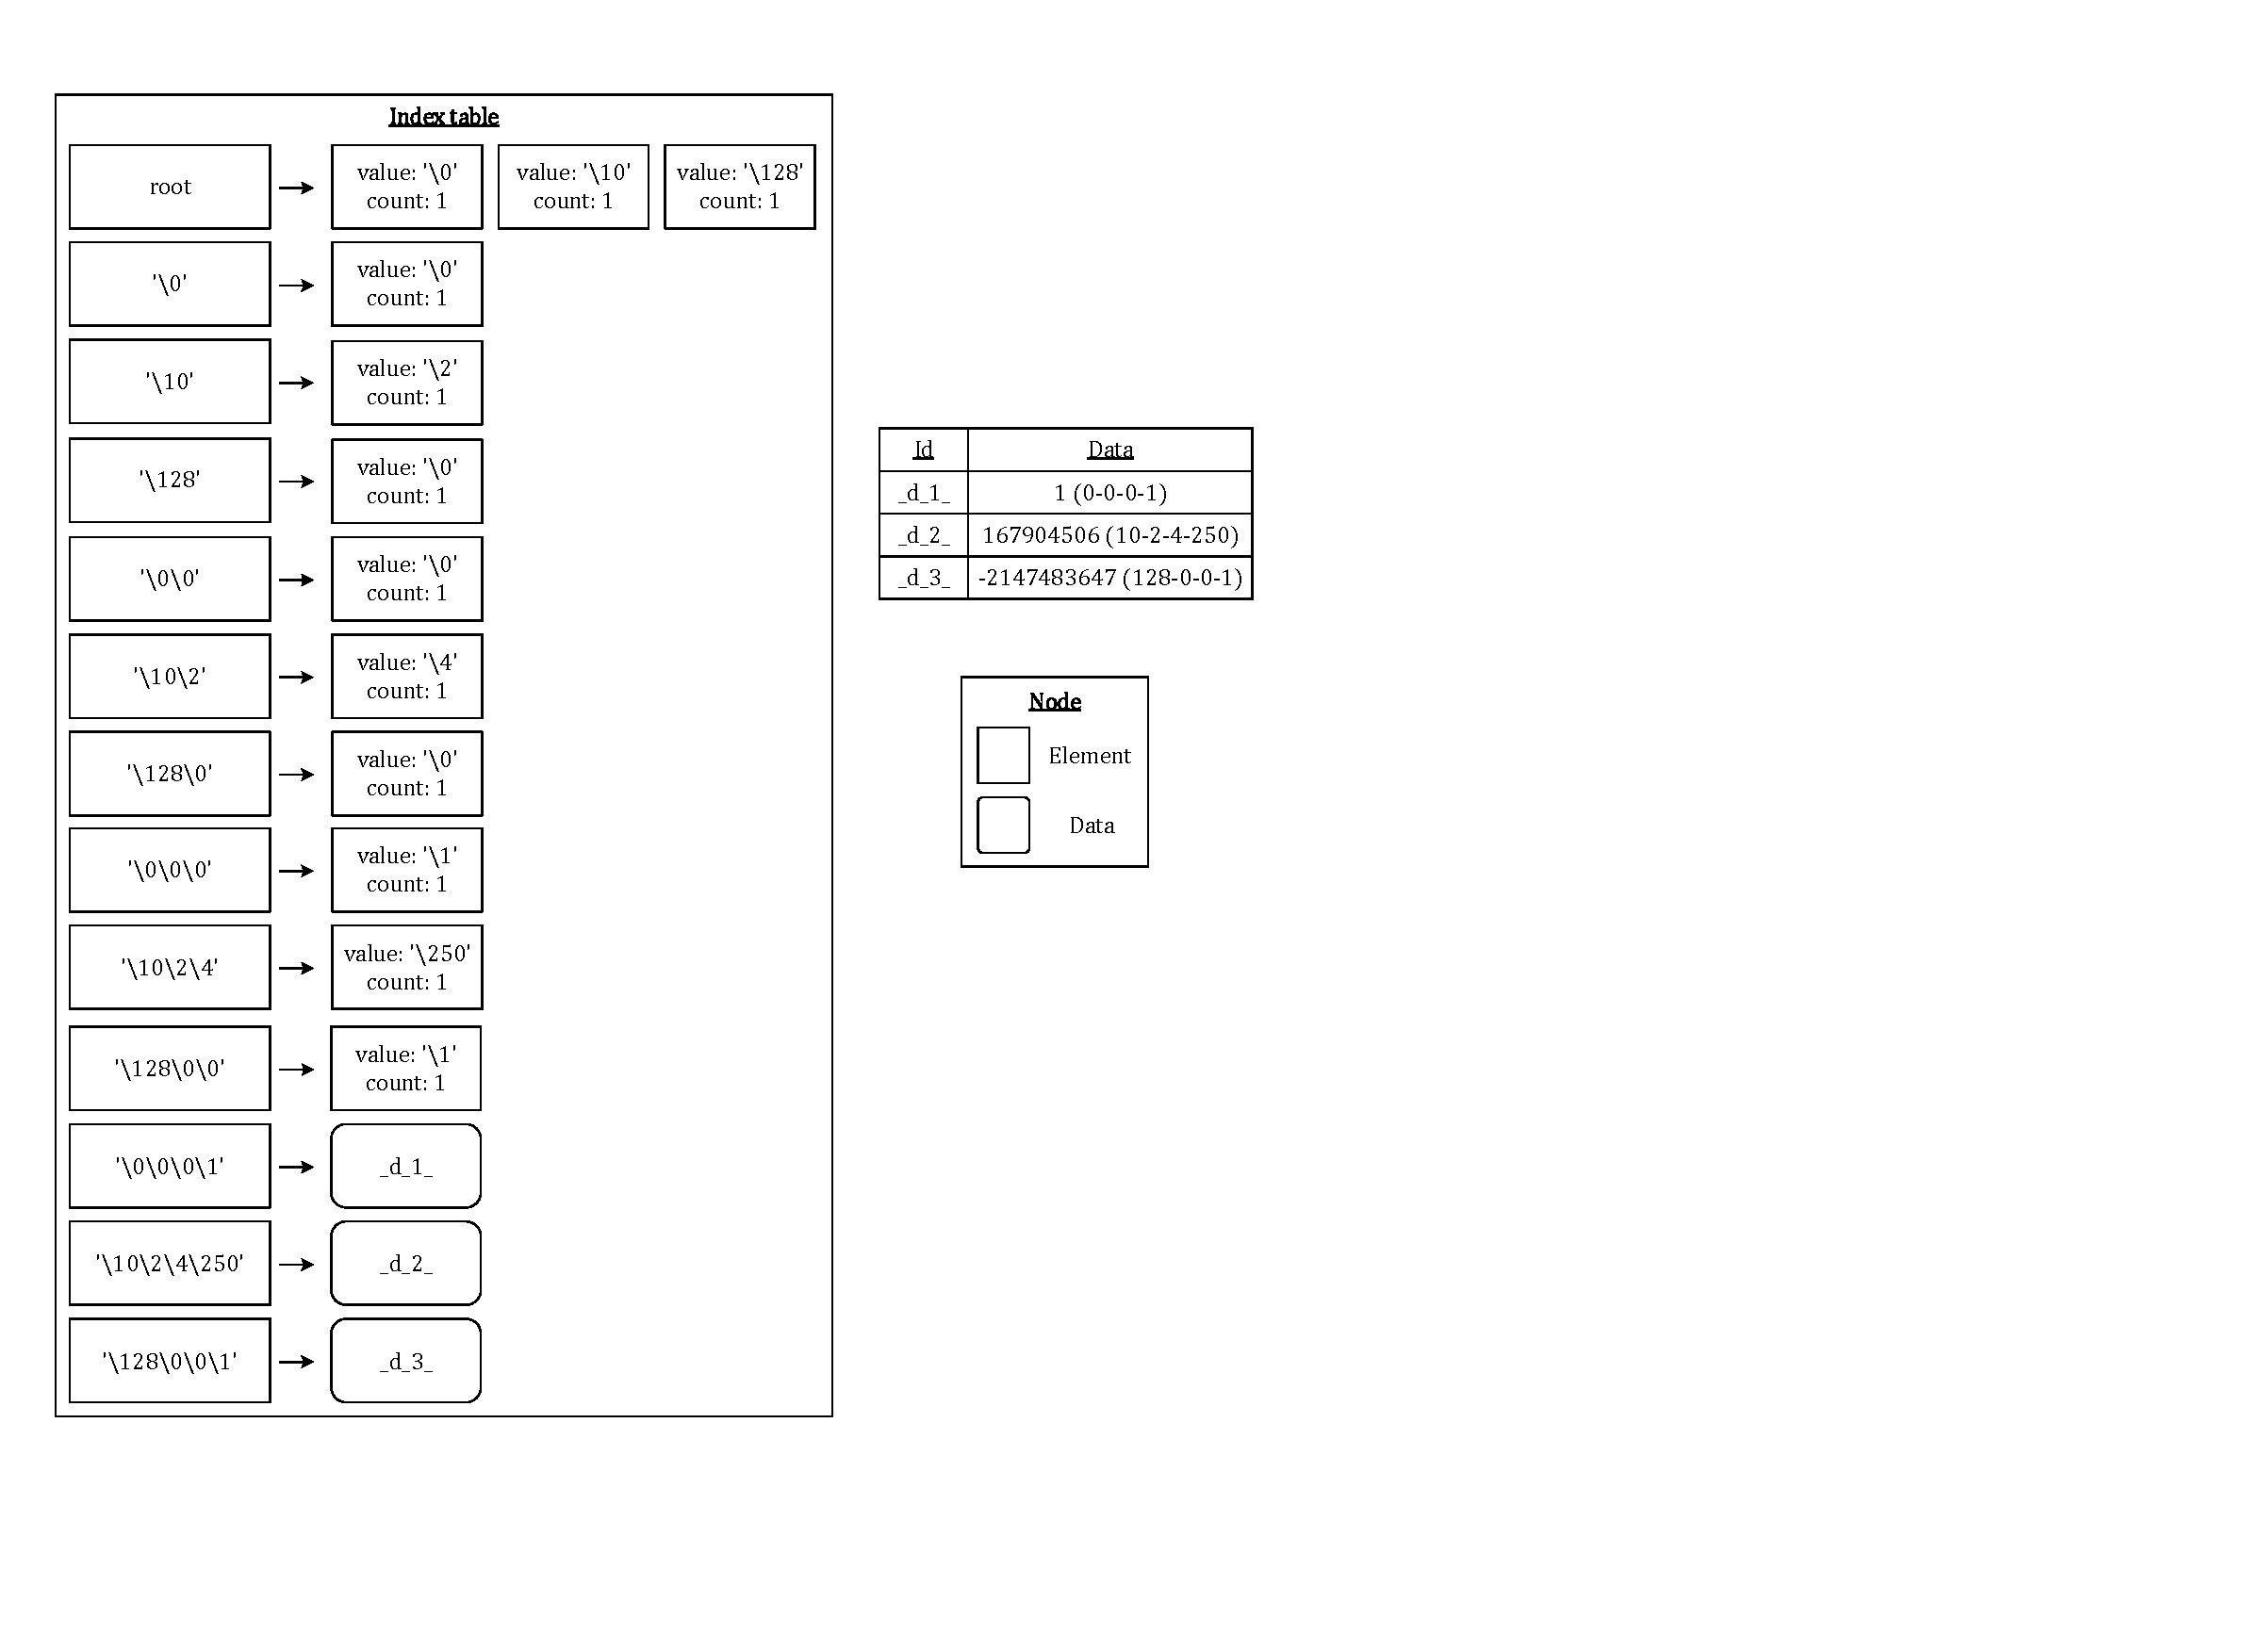
\includegraphics[width=0.8\textwidth]{./algorithm/integer/pic/insertion/example_1_v3.pdf}
\caption{The table after insert a negative value.}
\label{fig:algorithm:integer:insertion:example_1}
\end{figure}

Figure \ref{fig:algorithm:integer:insertion:example_1} shows that even a negative value will store as the same way as the positive value. And time complexity is $O(b)$.



% Deletion section
\subsubsection{Deletion}

Deletion is just do the opposite insertion to remove the byte and decrease the count. Fellow the same rule, if the count become zero, then the node will be remove. The time complexity is also $O(b)$.


% Modification section
\subsubsection{Modification}

The modify flow are similar as \textit{STRING} type, remove the key which don't needed and add the count if the byte is the same. So follow the example in figure \ref{fig:algorithm:integer:insertion:example_1} and modify 167904506 (10-2-4-250) to 2 (0-0-0-2), the table will look like figure \ref{fig:algorithm:integer:modification:example_1} and time complexity is $O(b)$.

\begin{figure}[h]
\centering
%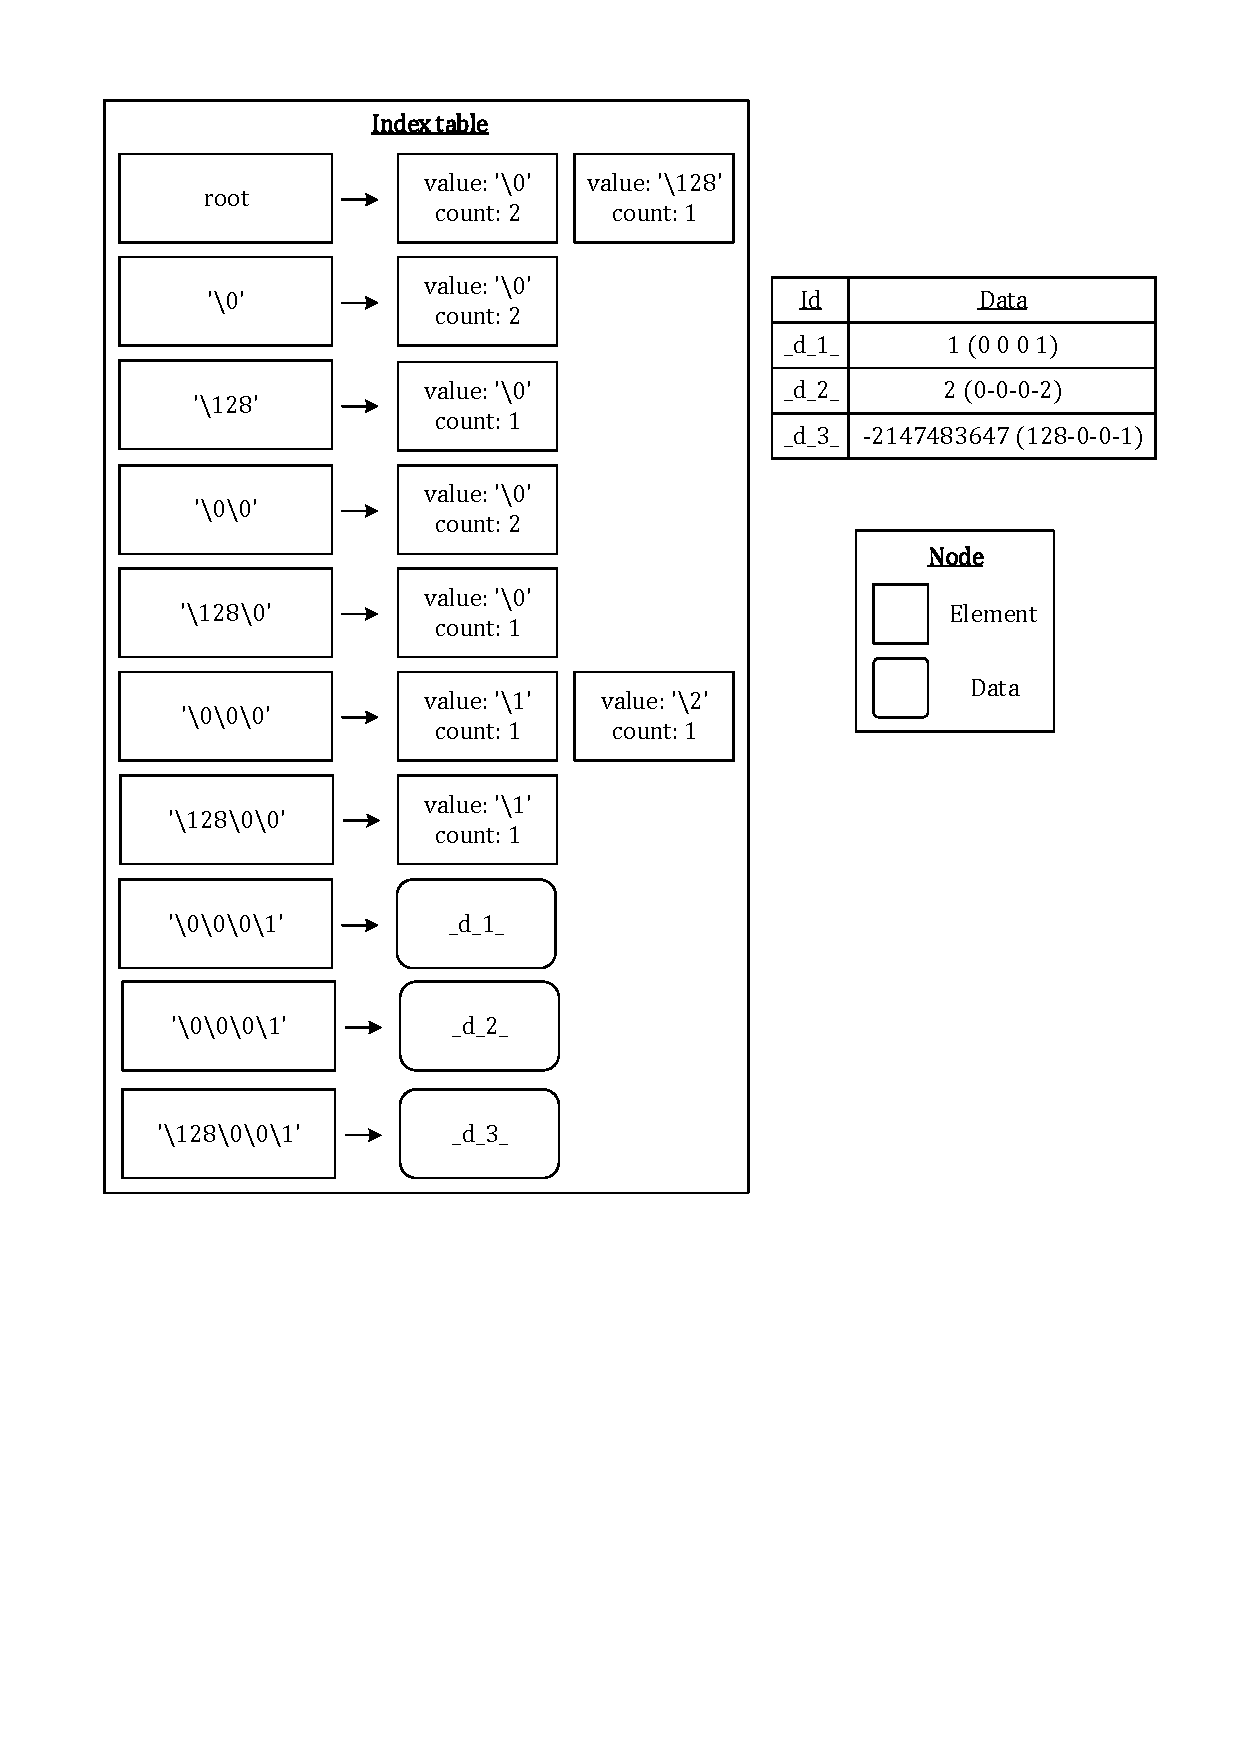
\includegraphics[scale=0.6]{./algorithm/integer/pic/modification/example_1_v3.pdf}
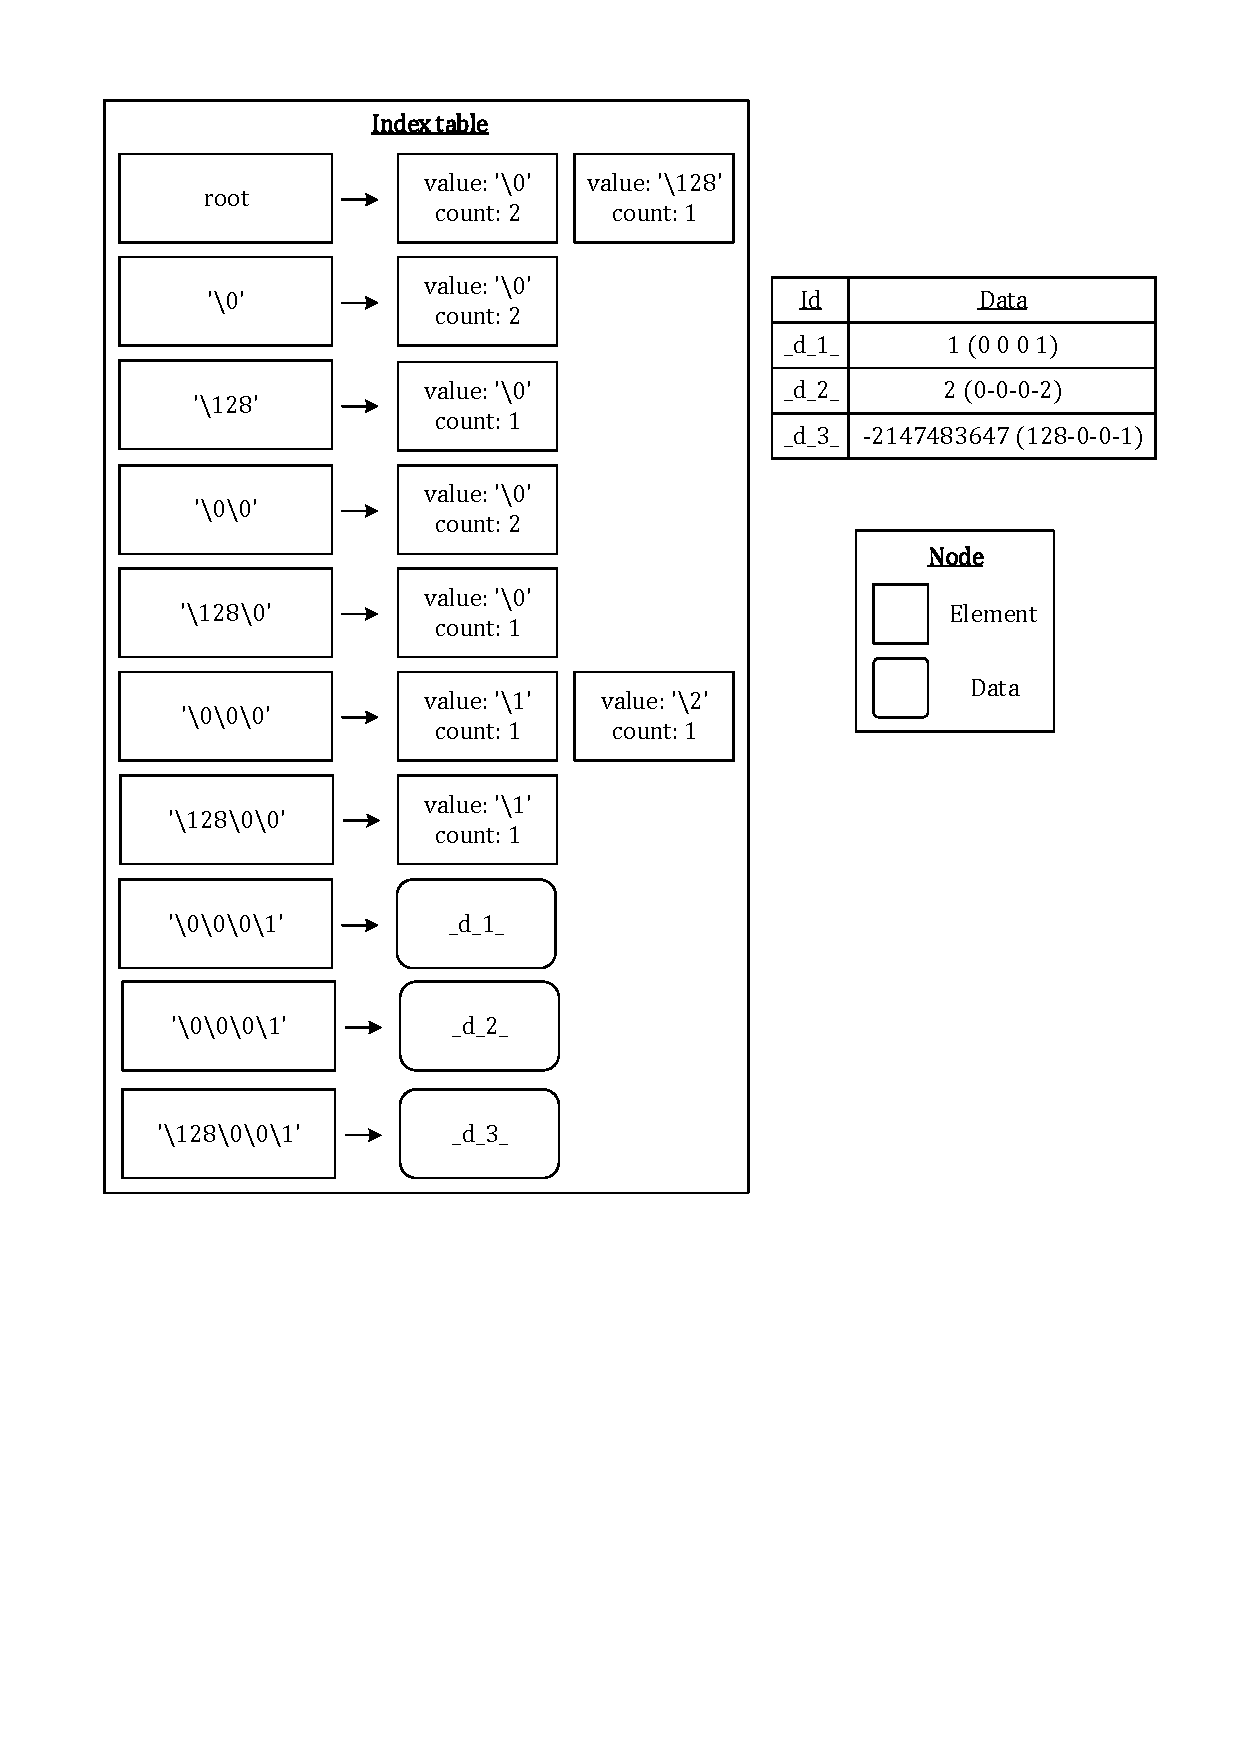
\includegraphics[width=0.8\textwidth]{./algorithm/integer/pic/modification/example_1_v3.pdf}
\caption{The table after modified the value.}
\label{fig:algorithm:integer:modification:example_1}
\end{figure}



% Selection section
\subsubsection{Selection}

Normally the database proves some function for compare the value of searching, so the Li's Hash musts also can do the same thing.

We use figure \ref{fig:algorithm:integer:modification:example_1} as example to demo the selection.

% Selection section enumerate
\begin{enumerate}

% --------------------------------------------------------

% Equal section
\item \textbf{Equal}

Compare the value is very simple. For example if we want to find data is equal to \textit{1 (0-0-0-1)}, we just need to use the key as $'\backslash0\backslash0\backslash0\backslash1'$ to search the index table. This should only take the time as $O(1)$.

% --------------------------------------------------------

% Not equal section
\item \textbf{Not equal}

Because it can't directly use the input value as key. So in this operation, it will start with the root key and parse all the result to find these element node until find the data node, but skip checking the key is as same as the input value. The time complexity be $O(b)$.

% --------------------------------------------------------

% Less than section
\item \textbf{Less than}

The \emph{"Less than"} comparison is similar as \emph{"Not equal"} comparison.

% Less than section description
\begin{description}

% Unsigned section
\item \textbf{Unsigned}

Start from root key, skip all the value which is \textit{"greater than"} the input value of the first byte, for example if the table contain \textit{10-X-X-X}, \textit{15-X-X-X} and \textit{20-X-X-X}, then if the input value is \textit{15-X-X-X}, the result will remain \textit{10-X-X-X} and \textit{15-X-X-X}. After that, search until to the last byte, then check the first byte if it is equal to the first byte of input value, and skip all the last byte which is \textit{"greater than or equal to"} the last byte of input value, otherwise keep all the result.

% Signed section
\item \textbf{Signed}

% Signed section enumerate
\begin{enumerate}

% Input value is a negative value
\item \textbf{Input value is a negative value}

If the input is a negative, then only start from the first byte is \textit{"greater than or equal to"} the inputs' first byte, and skip the key as same as the input.

% Input value is a positive value
\item \textbf{Input value is a positive value}

If the input is a positive, then start from the first byte is \textit{"less than or equal to"} the inputs' first byte and also skip the first byte is \textit{"greater than or equal to"} $\backslash128$ and the key as same as the input.

% Input value is equal to 0.0
\item \textbf{Input value is equal to 0.0}

If the input is zero, then then start from the first byte is \textit{"greater than or equal to"} $\backslash128$.

% End Signed section enumerate
\end{enumerate}

% End Less than section description
\end{description}

The \emph{"Less than or equal to"} comparison is just do the \emph{"Less than"} and \emph{"Equal"} operation and then combine both result for ouput. The time complexity is $O(b)$ for both operation.

% --------------------------------------------------------

% Greater than section
\item \textbf{Greater than}

This comparison flow is same as \emph{"Less than"}, and just need to convert all the \textit{"greater than"} to \textit{"less than"} and \textit{"less than"} to \textit{"greater than"}, the \emph{"Greater than or equal to"} will do the same thing. So time complexities are the same.

% --------------------------------------------------------

% Between section
\item \textbf{Between}

The \emph{"Between"} comparison is combining \emph{"Less than or equal to"} and \emph{"Greater than or equal to"} operation.

% Between section description
\begin{description}

% Unsigned section
\item \textbf{Unsigned}

Start with root key, but only keep the first byte which is only between and equal with the first byte of $minimum$ and $maximum$ input value.

For example if the table contain \textit{5-X-X-X}, \textit{10-X-X-X}, \textit{15-X-X-X}, \textit{20-X-X-X} and \textit{25-X-X-X}, and the input values are \textit{6-X-X-X} and \textit{20-X-X-X}, so \textit{10-X-X-X}, \textit{15-X-X-X} and \textit{20-X-X-X} are the result.

After that, search until to the last byte. Check the first byte if it is equal to the first byte of input value:

% Unsigned section enumerate
\begin{enumerate}[label=\bfseries \arabic*)]

\item When it is equal to the byte of $maximum$ input value, then skip all the last byte which is \textit{"greater than or equal to"} the last byte of $maximum$ input value.

\item When it is equal to the byte of $minimum$ input value, then skip all the last byte which is \textit{"less than or equal to"} the last byte of $minimum$ input value.

\item Otherwise keep all the result.

% End Unsigned section enumerate
\end{enumerate}


% Signed section
\item \textbf{Signed}

In signed integer, there are six cases for the \textbf{Between} operation:

% Signed section enumerate
\begin{enumerate}[label=\bfseries (\arabic*)]

% Case 1
\item \textbf{$minimum$ and $maximum$ are positive}

Use $minimum$ to do the \emph{"Greater than or equal to"}, and do \emph{"Less than or equal to"} by inputting the $maximum$. After that find the common result.

% Case 2
\item \textbf{$minimum$ and $maximum$ are negative}

As same as case \textbf{(1)}.

% Case 3
\item \textbf{$minimum$ is zero and $maximum$ is positive}

Use zero to do the \emph{"Greater than or equal to"}, and do \emph{"Less than or equal to"} by inputting the $maximum$. After that find the common result.

% Case 4
\item \textbf{$minimum$ is negative and $maximum$ is zero}

Use $minimum$ to do the \emph{"Greater than or equal to"}, and do \emph{"Less than or equal to"} by inputting the zero. After that find the common result.

% Case 5
\item \textbf{$minimum$ is negative and $maximum$ is positive}

Cut this into two part, the negative to zero part will do the \textbf{(4)}, another part will do \textbf{(3)}, after that find the common result.

% Case 6
\item \textbf{$minimum$ is positive value and $maximum$ are negative value}

This case should never happend because of the program should show warning message if the user really inputed like this.

% End Signed section enumerate
\end{enumerate}

The time complexity is $O(b)$.

% End Between section description
\end{description}
% --------------------------------------------------------

% End Selection section enumerate
\end{enumerate}



% Summary section
\subsubsection{Summary}

Table \ref{table:algorithm:integer:summary:time_complexity} is the summary the time complexity of each opration in \textit{INTEGER} type.

\begin{table}[h]
\centering
\caption{Time complexity for \textit{INTEGER} type.}
\label{table:algorithm:integer:summary:time_complexity}
\begin{tabular}{|c|c|}

\hline
\multicolumn{1}{|c|}{Operation} &
\multicolumn{1}{c|}{\tabincell{c}{
Time complexity \\ ($b$: The byte length of data, $b$ = 8)
}} \\

\hline
\multicolumn{1}{|c|}{Insert} &
\multicolumn{1}{c|}{$O(b)$)} \\

\hline
\multicolumn{1}{|c|}{Modify} &
\multicolumn{1}{c|}{$O(b)$)} \\

\hline
\multicolumn{1}{|c|}{Delete} &
\multicolumn{1}{c|}{$O(b)$)} \\

\hline
\multicolumn{1}{|c|}{Equal} &
\multicolumn{1}{c|}{$O(1)$} \\

\hline
\multicolumn{1}{|c|}{\tabincell{c}{Equal (muti-value)}} &
\multicolumn{1}{c|}{$O(1)$} \\

\hline
\multicolumn{1}{|c|}{Not equal} &
\multicolumn{1}{c|}{$O(b)$)} \\

\hline
\multicolumn{1}{|c|}{\tabincell{c}{Not equal (muti-value)}} &
\multicolumn{1}{c|}{$O(b)$)} \\

\hline
\multicolumn{1}{|c|}{Less than} &
\multicolumn{1}{c|}{$O(b)$)} \\

\hline
\multicolumn{1}{|c|}{Less than or equal} &
\multicolumn{1}{c|}{$O(b)$)} \\

\hline
\multicolumn{1}{|c|}{Greater than} &
\multicolumn{1}{c|}{$O(b)$)} \\

\hline
\multicolumn{1}{|c|}{Greater than or equal} &
\multicolumn{1}{c|}{$O(b)$)} \\

\hline
\multicolumn{1}{|c|}{Between} &
\multicolumn{1}{c|}{$O(b)$)} \\

\hline
\end{tabular}
\end{table}


\clearpage


% REAL section
\subsection{REAL type}

From 1960, there are many computer company has they own design of floating point, this cause a huge problem in data exchange andcommunication, this bring out the standard of IEEE 754 \cite{web:wiki:ieee-754}. Because of the hardware design, if want to have a range of the data, then it need to sacrifice the accuracy, this called the "Round-off error" \cite{web:wiki:round-off_error,web:c:handle-round-off_error}.\\

That's why the IEEE 754 specific the best between range and the accuracy, but still it can't provide 100\% accuracy, also the design of IEEE 754 is not suitable for do the operation like sorting and comparison. So if want to handle the data as a floating point, then this need to jump out from the IEEE 754, and building the own data structure. Then this can store the data no matter how big it is with 100\% accuracy, but this cost a little more space.\\

We study the design and description of $float$ and $double$ design from some of the existing relational database \cite{web:wiki:floating_point,web:wiki:double-precision_floating-point_format,web:wiki:real-number,web:vcpp:data-type-ranges,web:wiki:c-data-types,web:c:data-types,web:transact-sql:int-bigint-smallint-tinyint,web:transact-sql:effective_number_of_bits-decimal_places-length,web:transact-sql:float-real,web:csharp:decimal,web:sql-server:decimal-float-real,web:c-cpp:floating-point-precision,web:mysql:query-sorting-numbers,web:mysql:using-decimal-to-record-float-point,web:mysql:sql-manual-reference}. In these database, they usually design a data type as \textit{"Decimal"} to handle the problem of IEEE 754.\\

\textit{"Decimal"} is a unpack floating point which contain the sign, and the number are store as a string, this means each number will consume a byte to record it. When need to do sorting or comparison operation, it will need to read the data and convert it into string first, this means it need cost one more step before the process.\\

So if fellow the \textit{"Decimal"} design to handle the floating point, this will cost more spaces. Such as if store "100" as \textit{"Decimal"} type which will as cost 3 bytes ('1', '0', '0'), but if using the character type (char) to store it which just need 1 byte ('d' in ASCII). Also we want the Li's Hash can use the index table can do the sorting or comparison, so we create a data type as \textit{REAL} to handle the problem above.\\

\textit{REAL} (aka the \textit{"real number"} in mathematics \cite{web:wiki:real-number}) is combine the concept of \textit{"Decimal"} and design of $INTEGER$. First convert the floating point into string when inputting the value, then partition it into three part to store as figure \ref{fig:algorithm:real:data_format}: \textit{"Sign"}, \textit{"Integer"}, \textit{"Decimal"}. After that convert \textit{"Integer"} and \textit{"Decimal"} part back into bytes by using base256, so this can use less byte to store the value, also this can use the design in $INTEGER$ to do indexing, so that \textit{REAL} can also do sorting or comparison operation. Also becuase need keep the accuracy of the value, so the length of byte usage is dynamic.\\

\begin{figure}[h]
\centering
%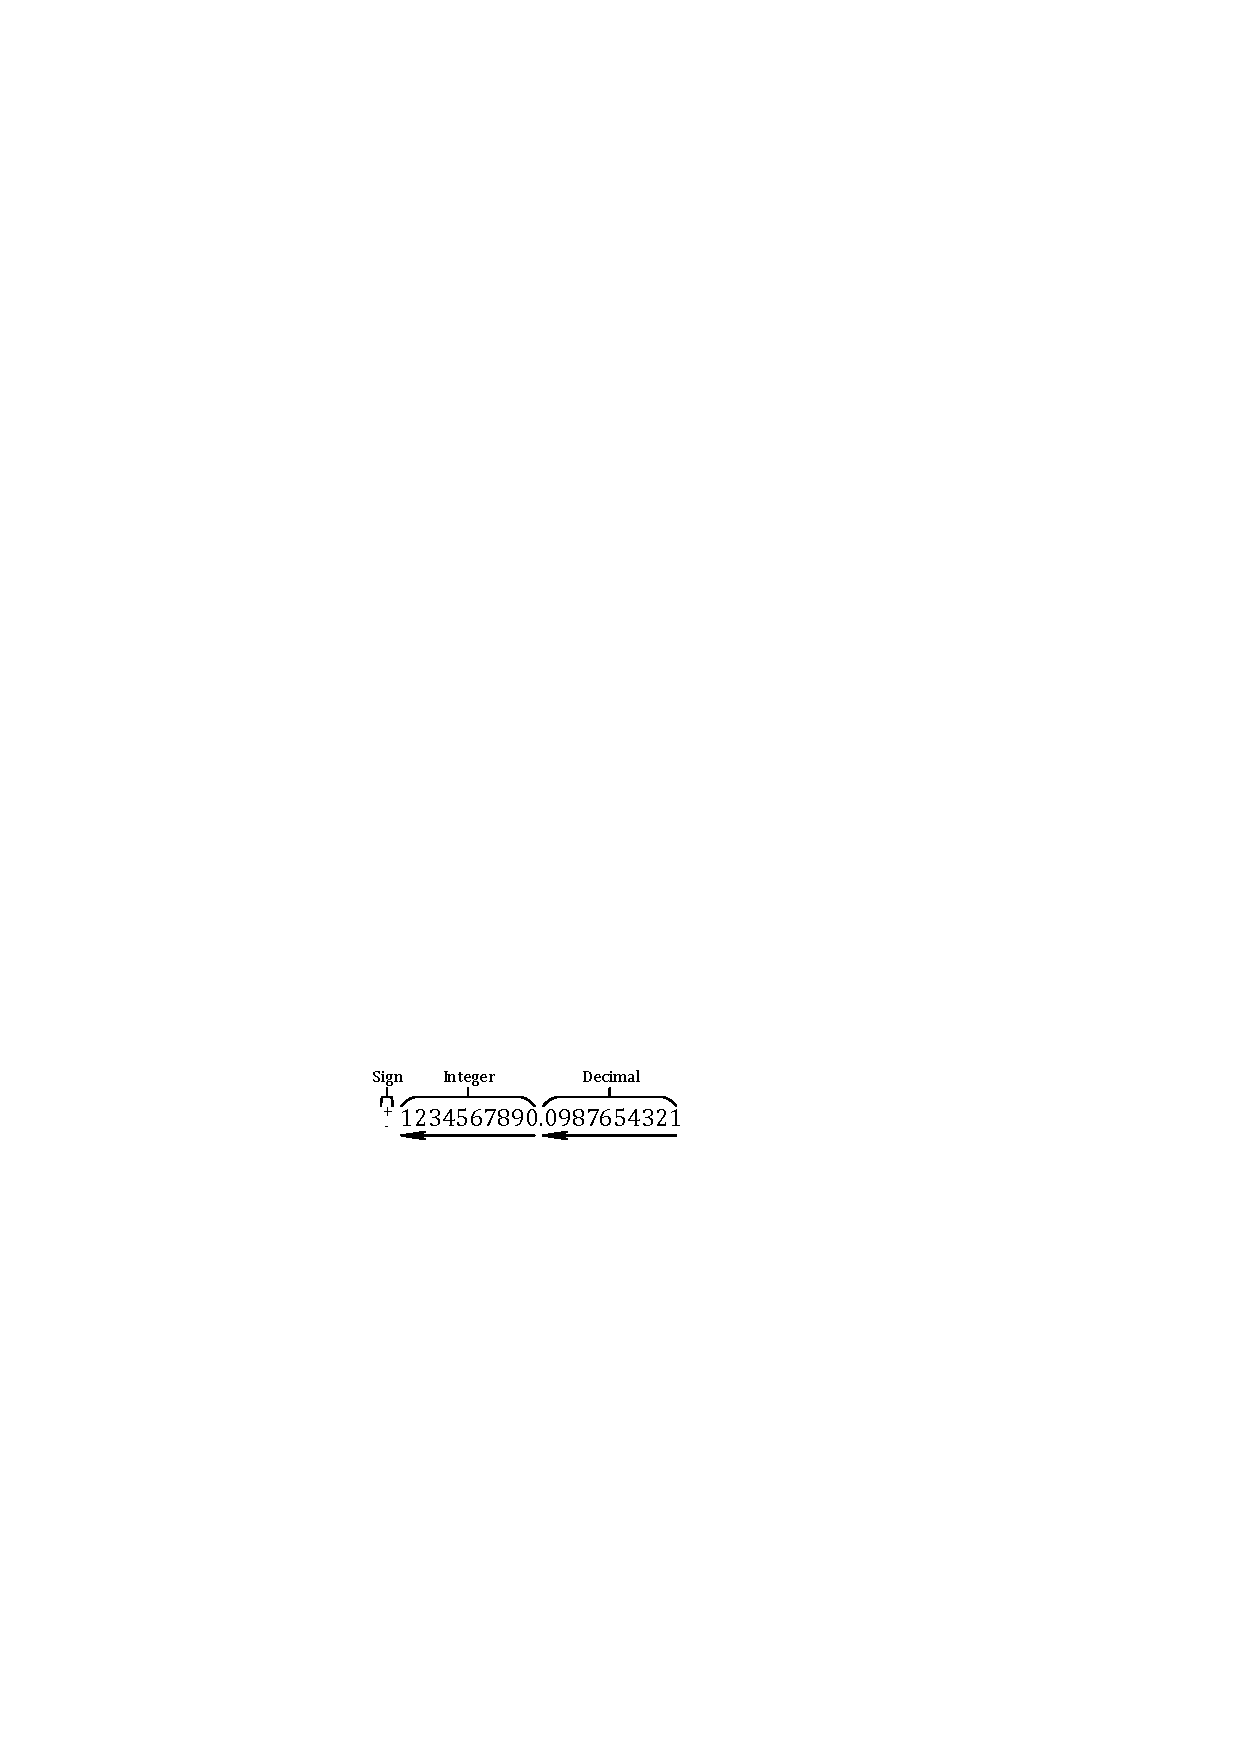
\includegraphics[scale=1.0]{./algorithm/real/pic/design/data_format_v3.pdf}
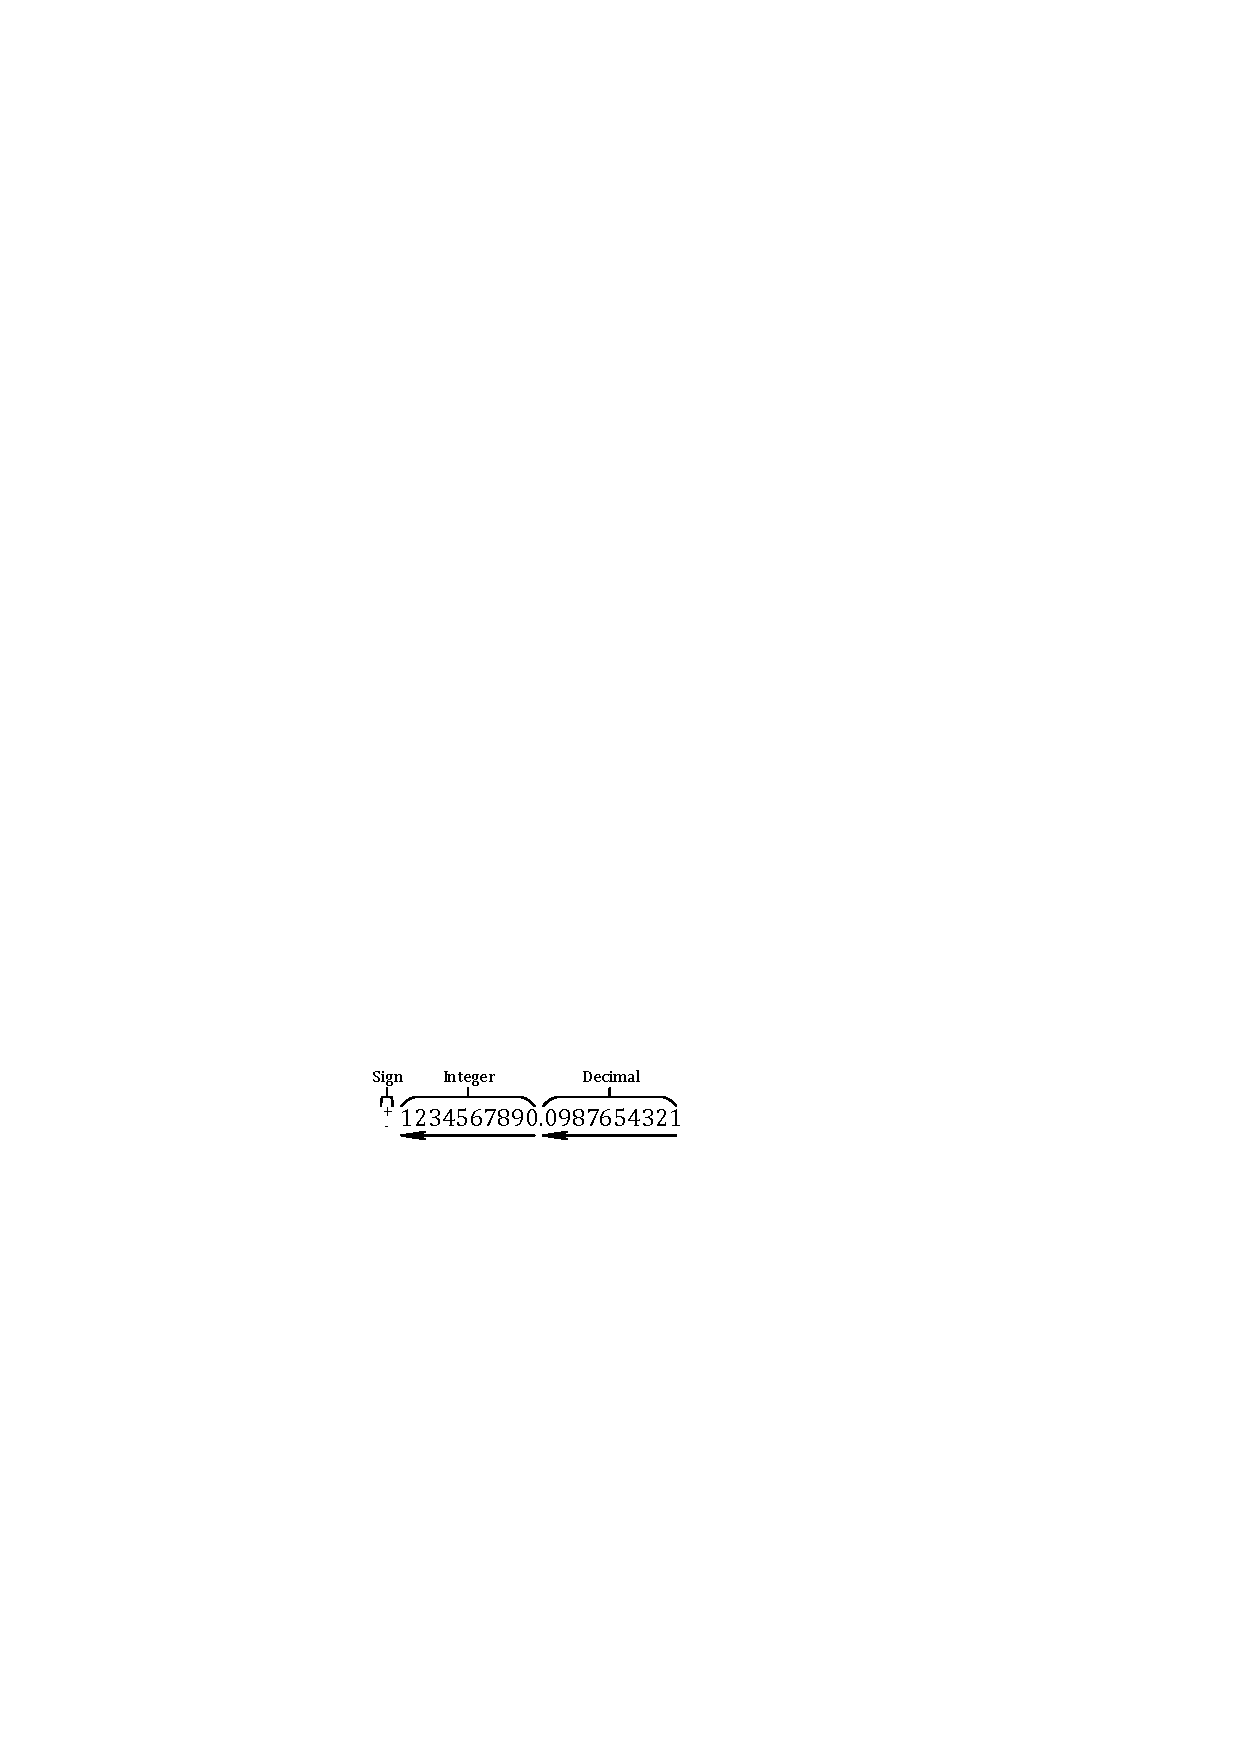
\includegraphics[width=0.6\textwidth]{./algorithm/real/pic/design/data_format_v3.pdf}
\caption{Data format of \textit{REAL} type.}
\label{fig:algorithm:real:data_format}
\end{figure}

The data format (figure \ref{fig:algorithm:real:data_format}) of \textit{REAL} is little bit different than the normal data concept, the value is as same as normal, the number at the left hand side means larger.\\

But when in the storage view is different, the \textit{"Integer"} part is store in normal and inverted order which will explain in the example of each operation, but the \textit{"Decimal"} part is using inverted which means the value will inverted when it stored. We use figure \ref{fig:algorithm:real:data_store_inverted} to explain why we do this.

\begin{figure}[h]
\centering
    \begin{subfigure}[b]{0.4\textwidth}
        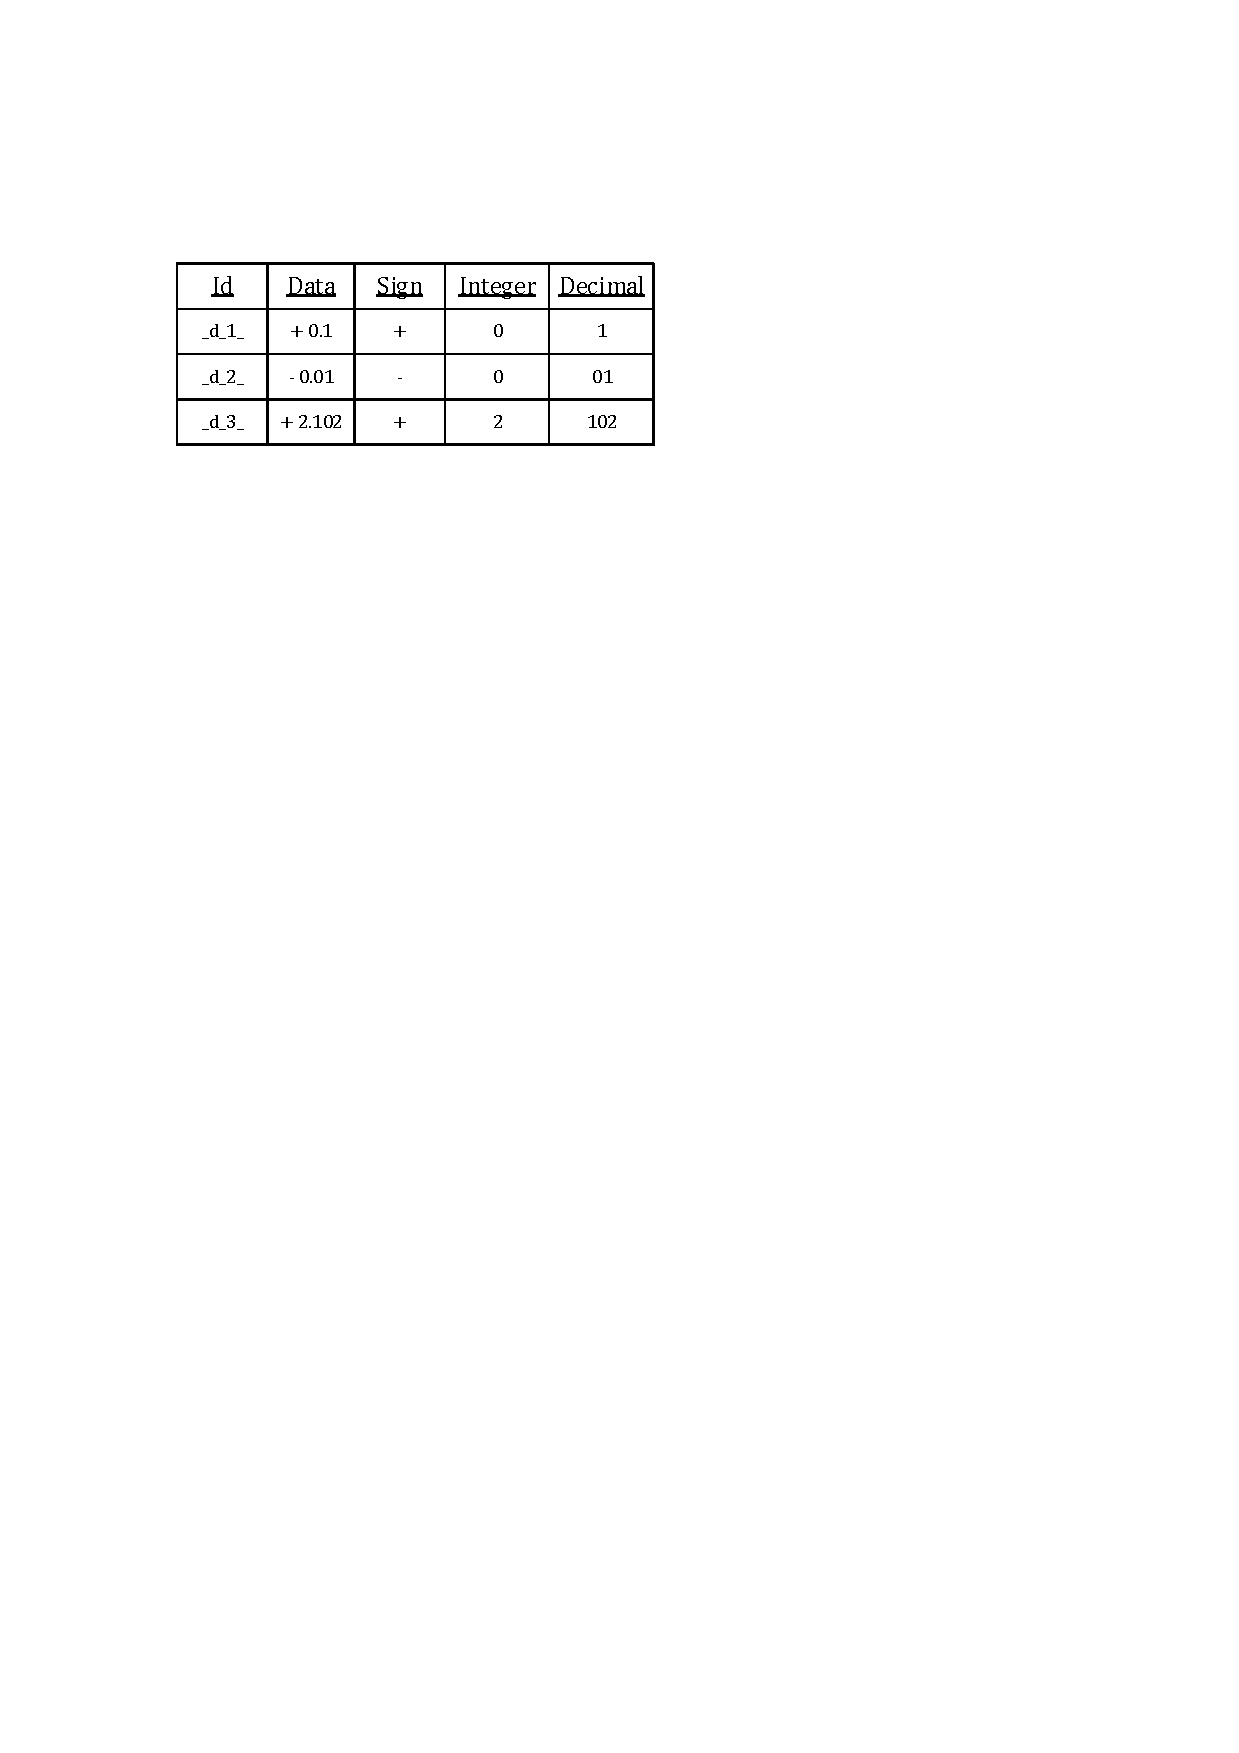
\includegraphics[width=\textwidth]{./algorithm/real/pic/design/data_store_inverted_1_v1.pdf}
        \caption{Normal order}
        \label{fig:algorithm:real:data_store_inverted_1}
    \end{subfigure}%
    ~ %add desired spacing between images, e. g. ~, \quad, \qquad etc.
          %(or a blank line to force the subfigure onto a new line)
    \begin{subfigure}[b]{0.4\textwidth}
        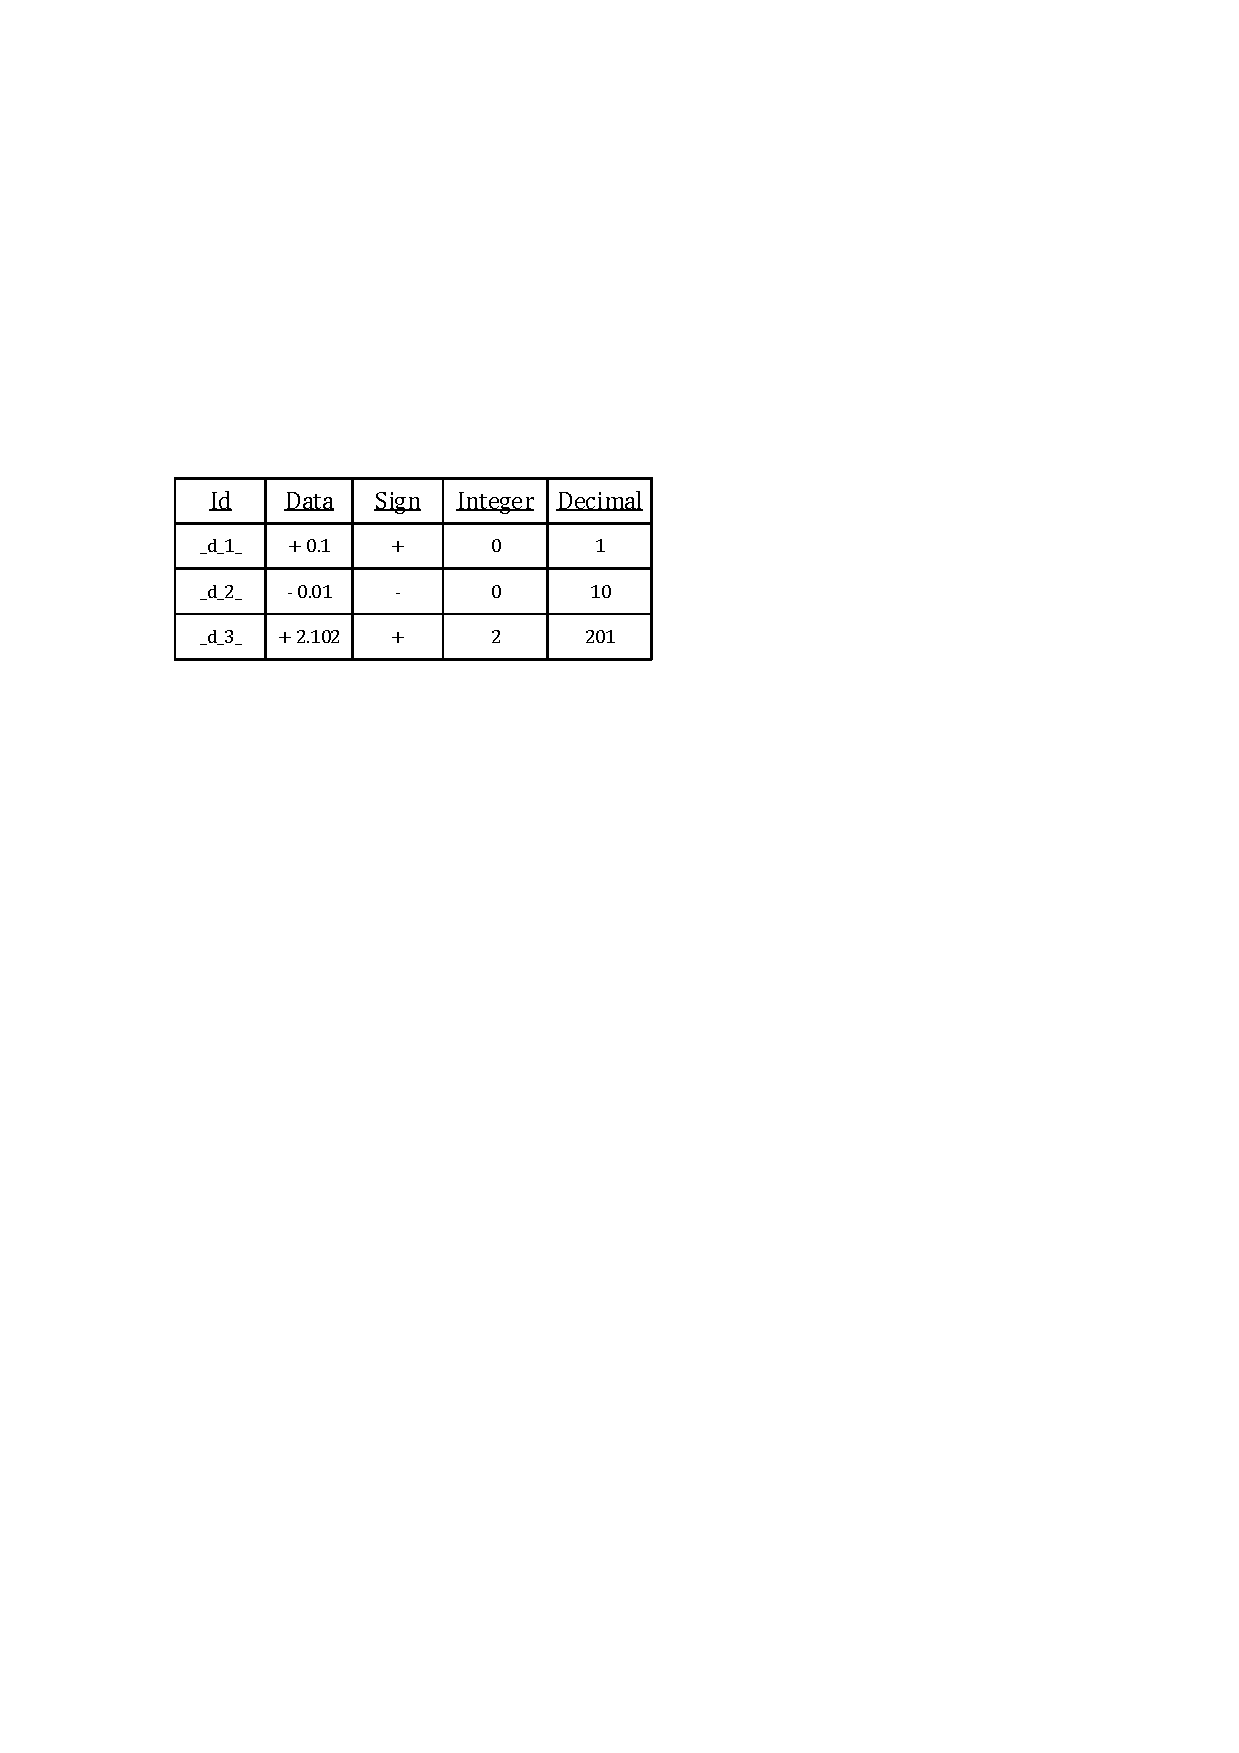
\includegraphics[width=\textwidth]{./algorithm/real/pic/design/data_store_inverted_2_v1.pdf}
        \caption{Inverted order}
        \label{fig:algorithm:real:data_store_inverted_2}
    \end{subfigure}

    \caption{Value storage}
    \label{fig:algorithm:real:data_store_inverted}
\end{figure}

If the data store as the same order as usual, the sample data will store like figure \ref{fig:algorithm:real:data_store_inverted_1}, the problem is if we treat \textit{'01'} as a value, it will convert into \textit{'1'} and lost its owns meaning, because \textit{'.1'} is not equal \textit{'.01'}. So if invert the \textit{"Decimal"} part, the value will look like figure \ref{fig:algorithm:real:data_store_inverted_2}. It shows the value can be store without missing value, the only is a additional convert operation is need to revert back into the real value when return data.\\

\begin{figure}[h]
\centering
%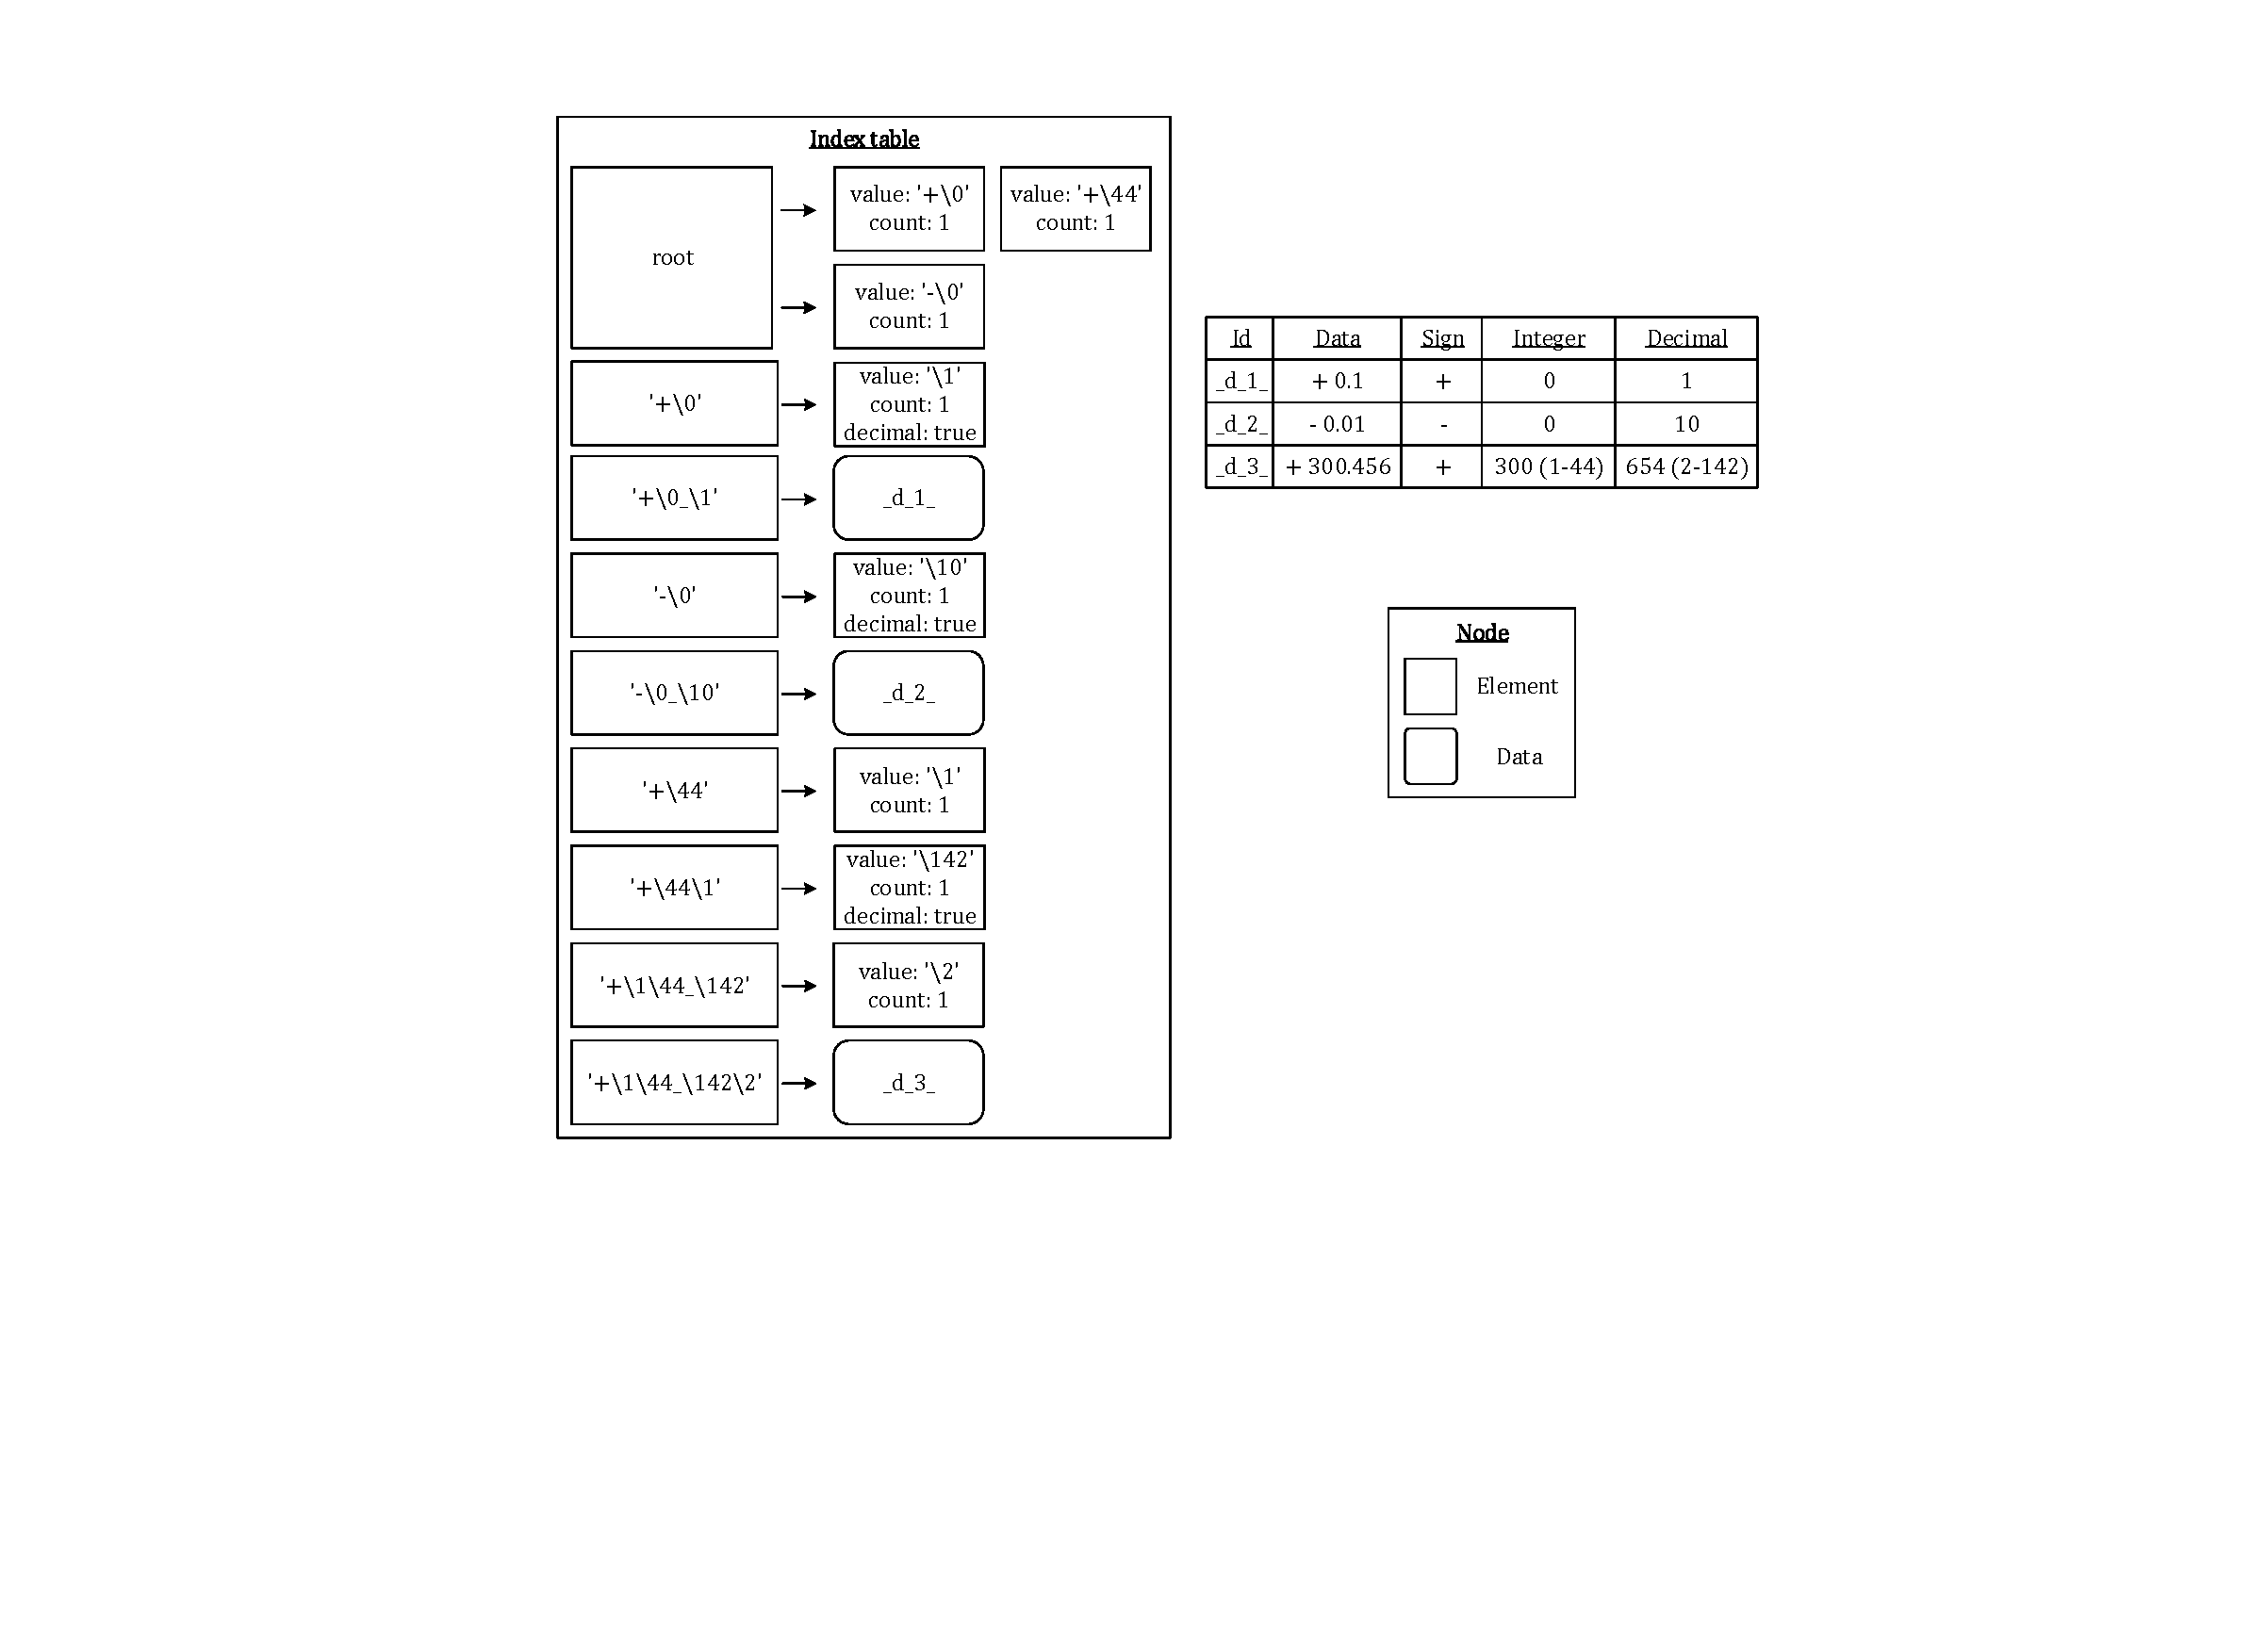
\includegraphics[scale=1.0]{./algorithm/real/pic/design/example_v4.pdf}
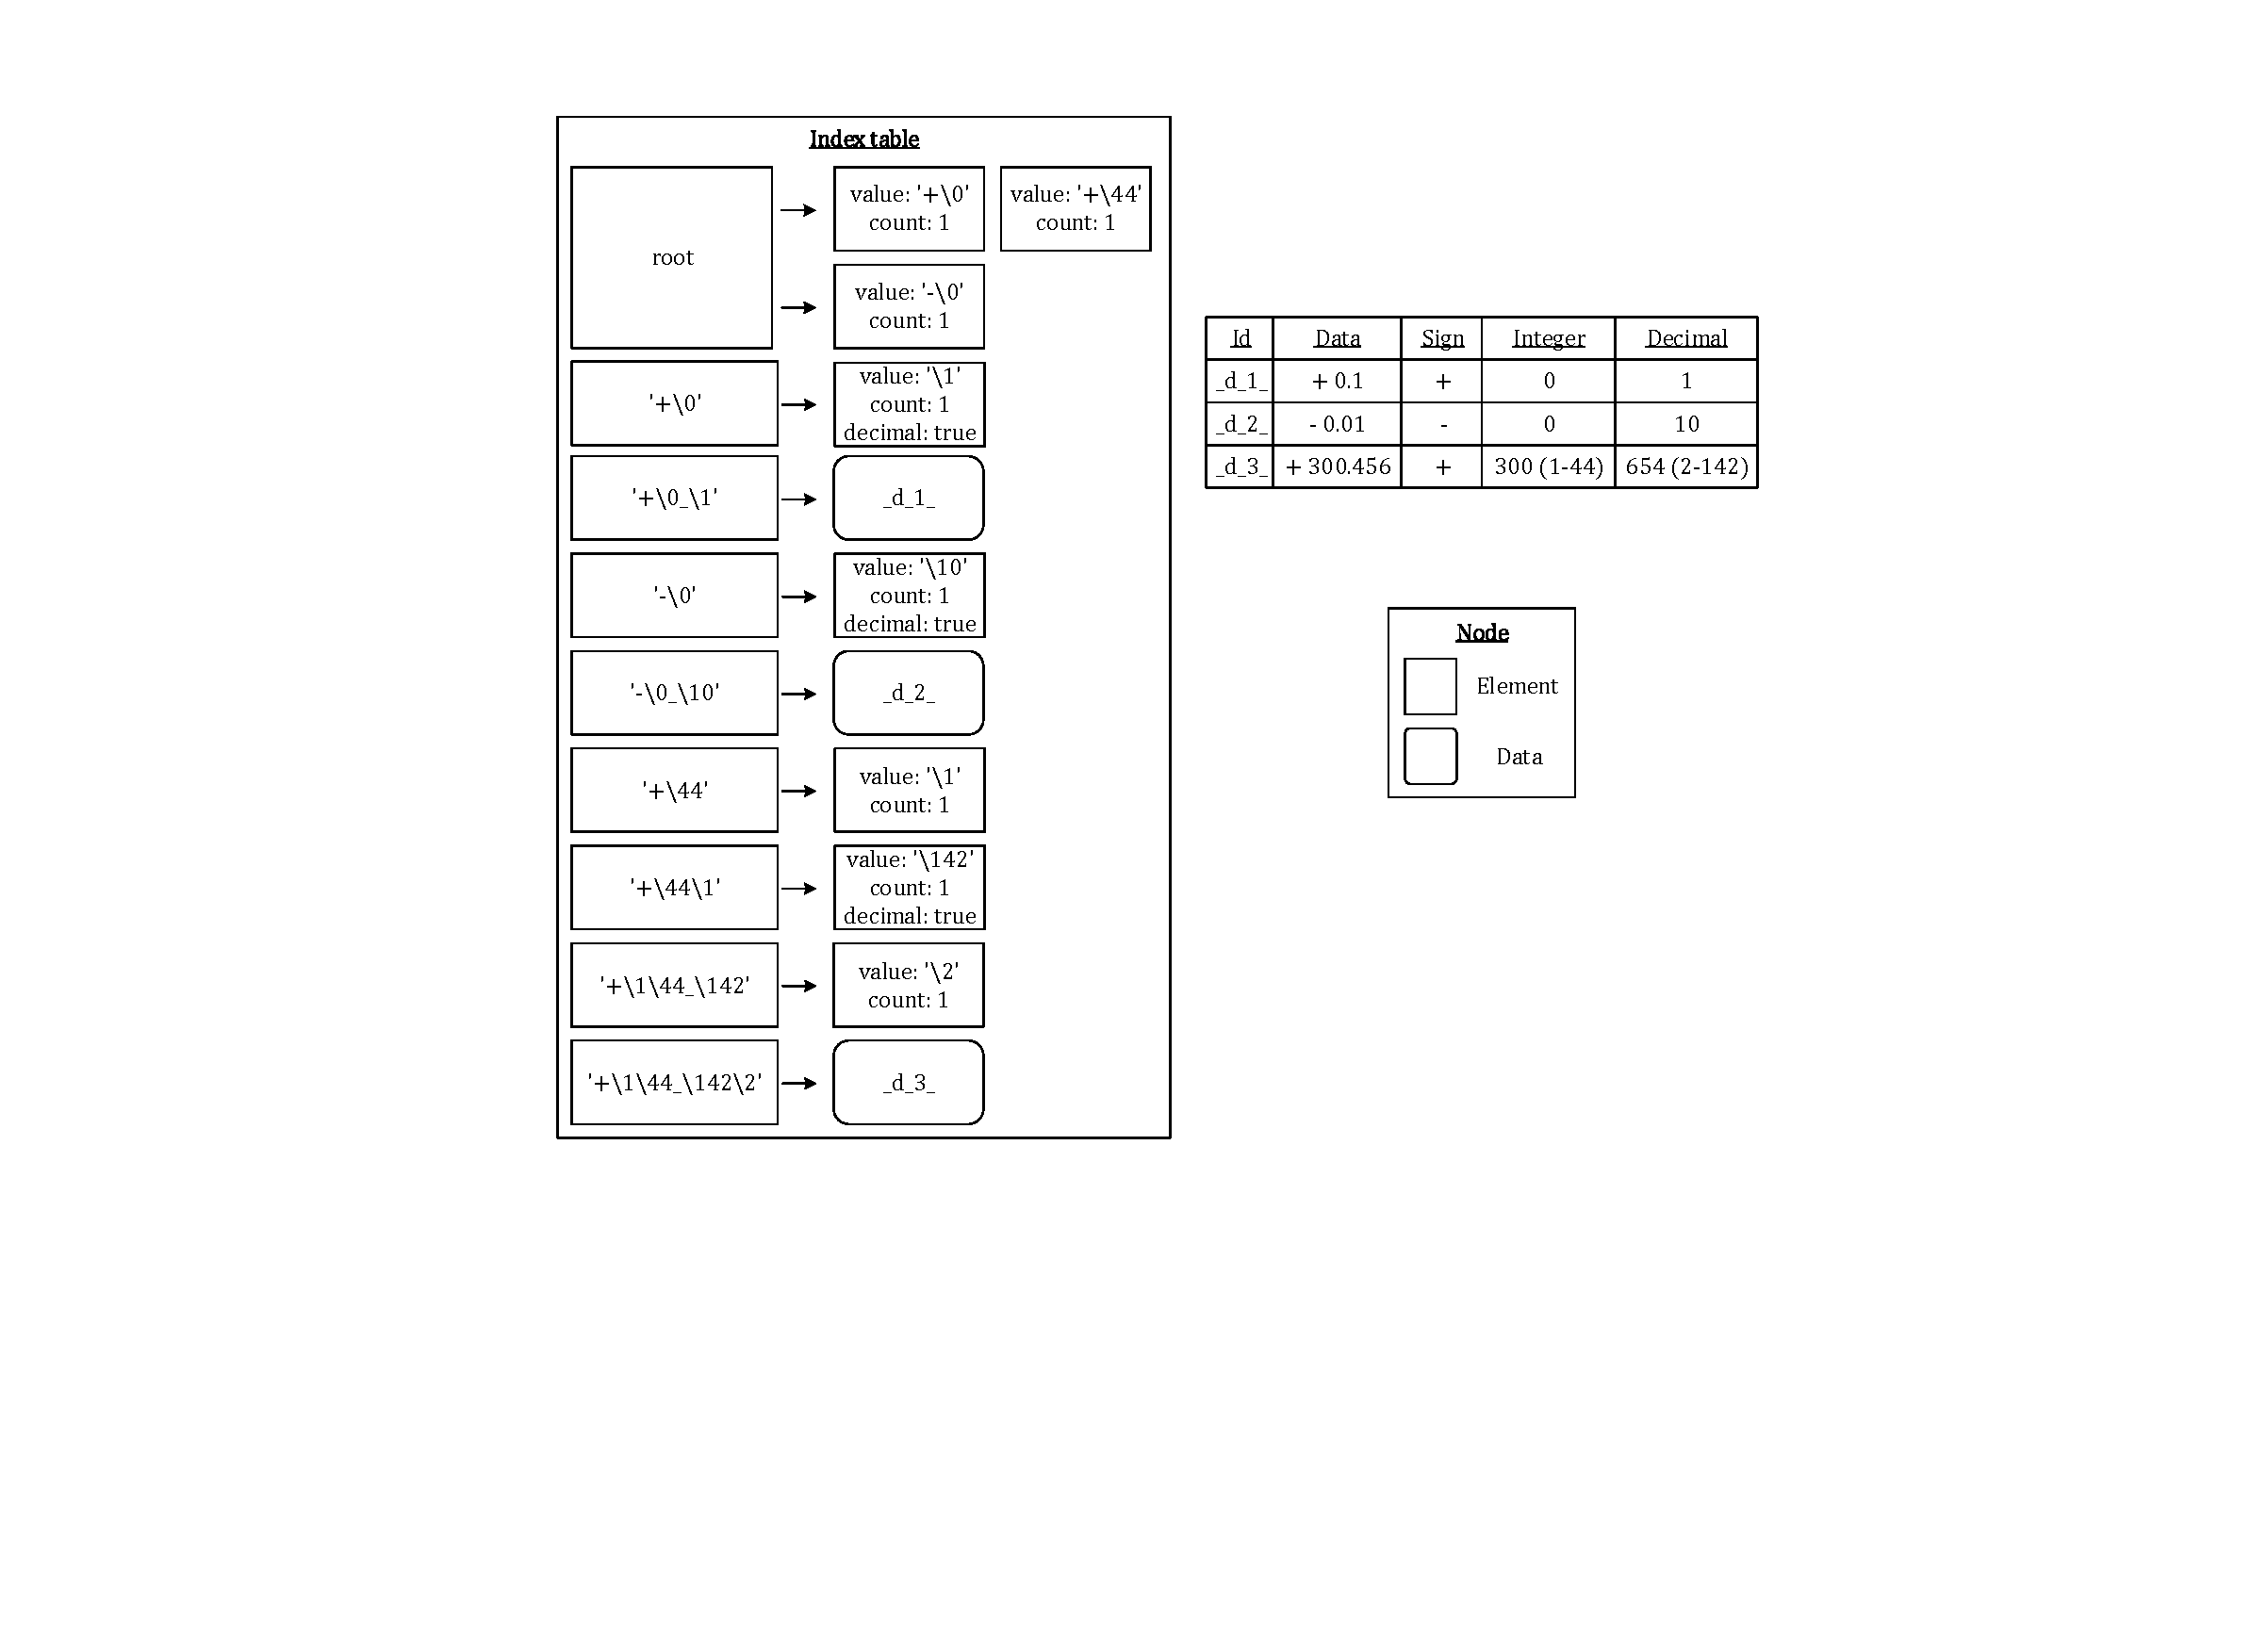
\includegraphics[width=0.8\textwidth]{./algorithm/real/pic/design/example_v4.pdf}
\caption{The index tables of \textit{REAL} type.}
\label{fig:algorithm:real:example}
\end{figure}

Figure \ref{fig:algorithm:real:example} is the example when storing data into index table. This table start with $root$ which is pointing to the \textit{"Sign"} part which is store with the last byte of \textit{"Integer"} part.

The \textit{"Integer"} is indexing using n-gram as normal, but it will index in two way:

\begin{enumerate}

\item When indexing the \textit{"Integer"} part only (like $'$+$\backslash44\backslash1'$ in figure), it is start from the last byte to the first, and then will pointing to the element node which contain a flag that means as $decimal$, which is represent to begin \textit{"Decimal"} part.

\item Like $'$+$\backslash1\backslash44\_\backslash2\backslash142'$ in figure, the order of the \textit{"Integer"} part is store as from the left to right when it is storing with the \textit{"Decimal"} part.

\end{enumerate}

And \textit{"Decimal"} is store from right to left, and because the inverted string value design which means if the value is small then it will become a greater value.

This order of \textit{"Integer"} and \textit{"Decimal"} part design is because this can do faster searching the key when doing sorting and comparison, this will explan detail in fellowing section.

% Insertion section
\subsubsection{Insertion}

In description and figure \ref{fig:algorithm:real:example} have already mentioned some of the flow of insertion, so in here will show the table if insert another value into the table. Insert $\pi (3.14159)$ into table, which will become like figure \ref{fig:algorithm:real:insertion:example}.

\begin{figure}[h]
\centering
%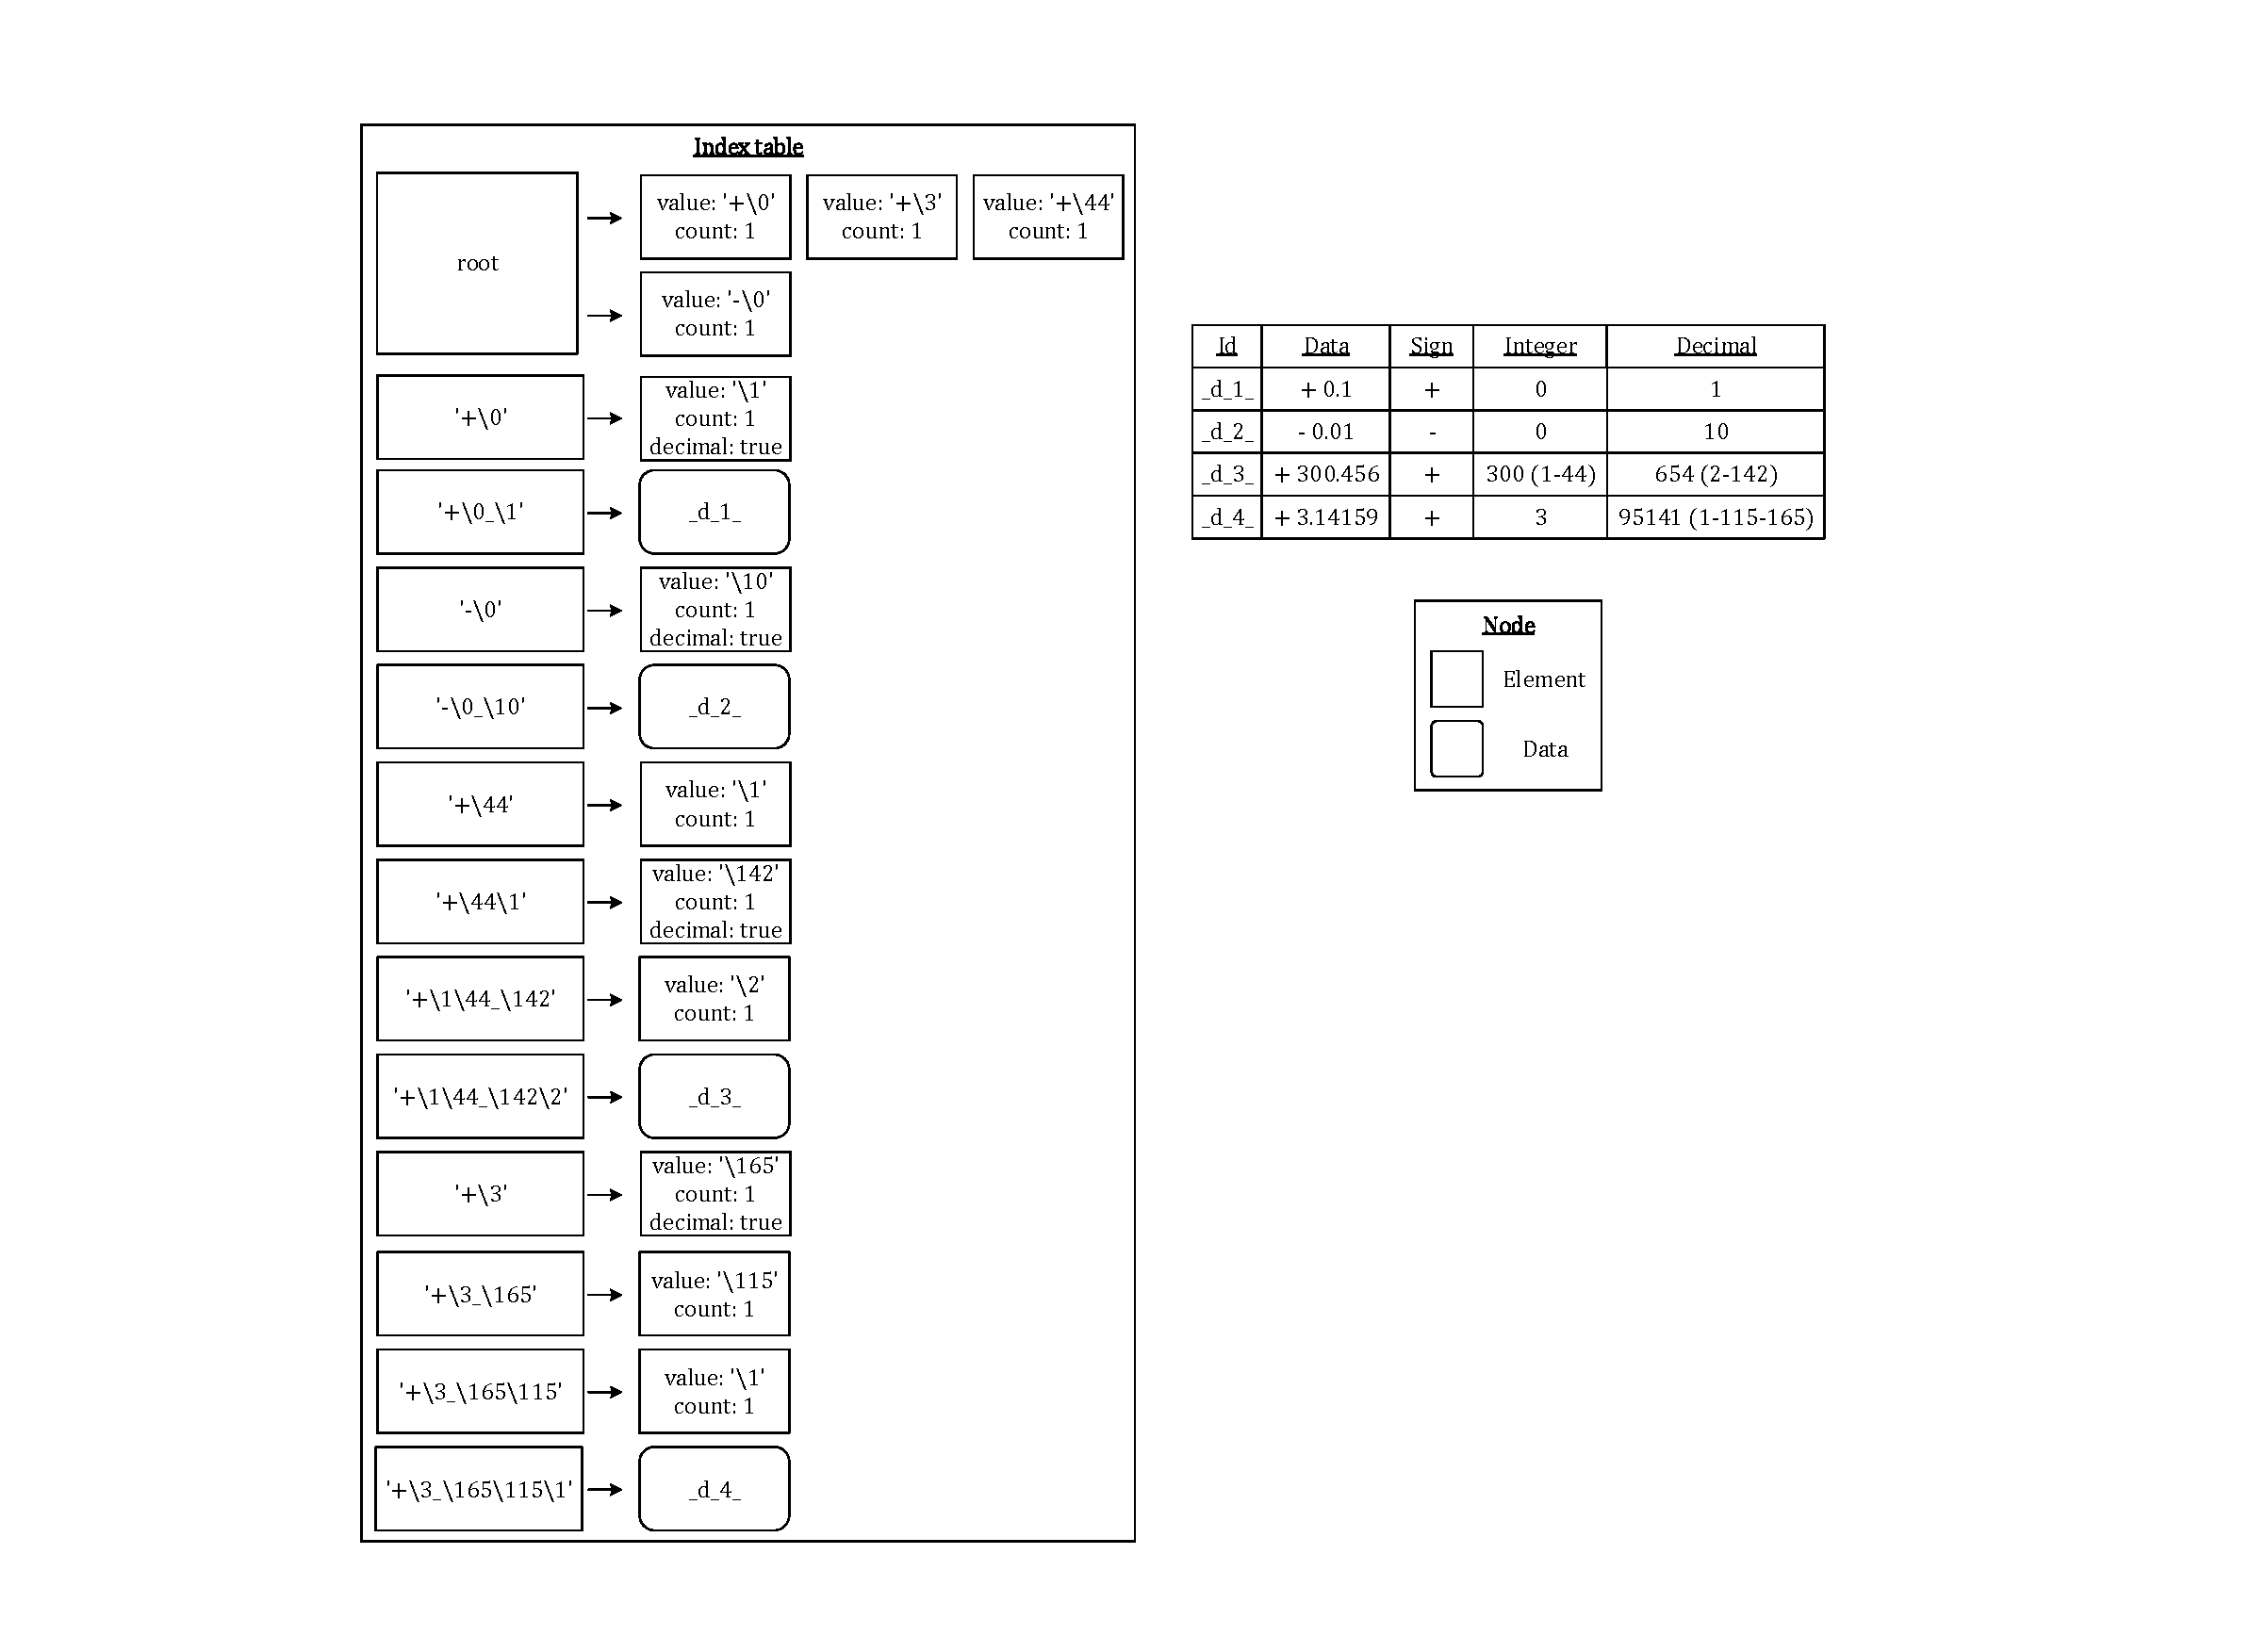
\includegraphics[scale=0.45]{./algorithm/real/pic/insertion/example_v4.png}
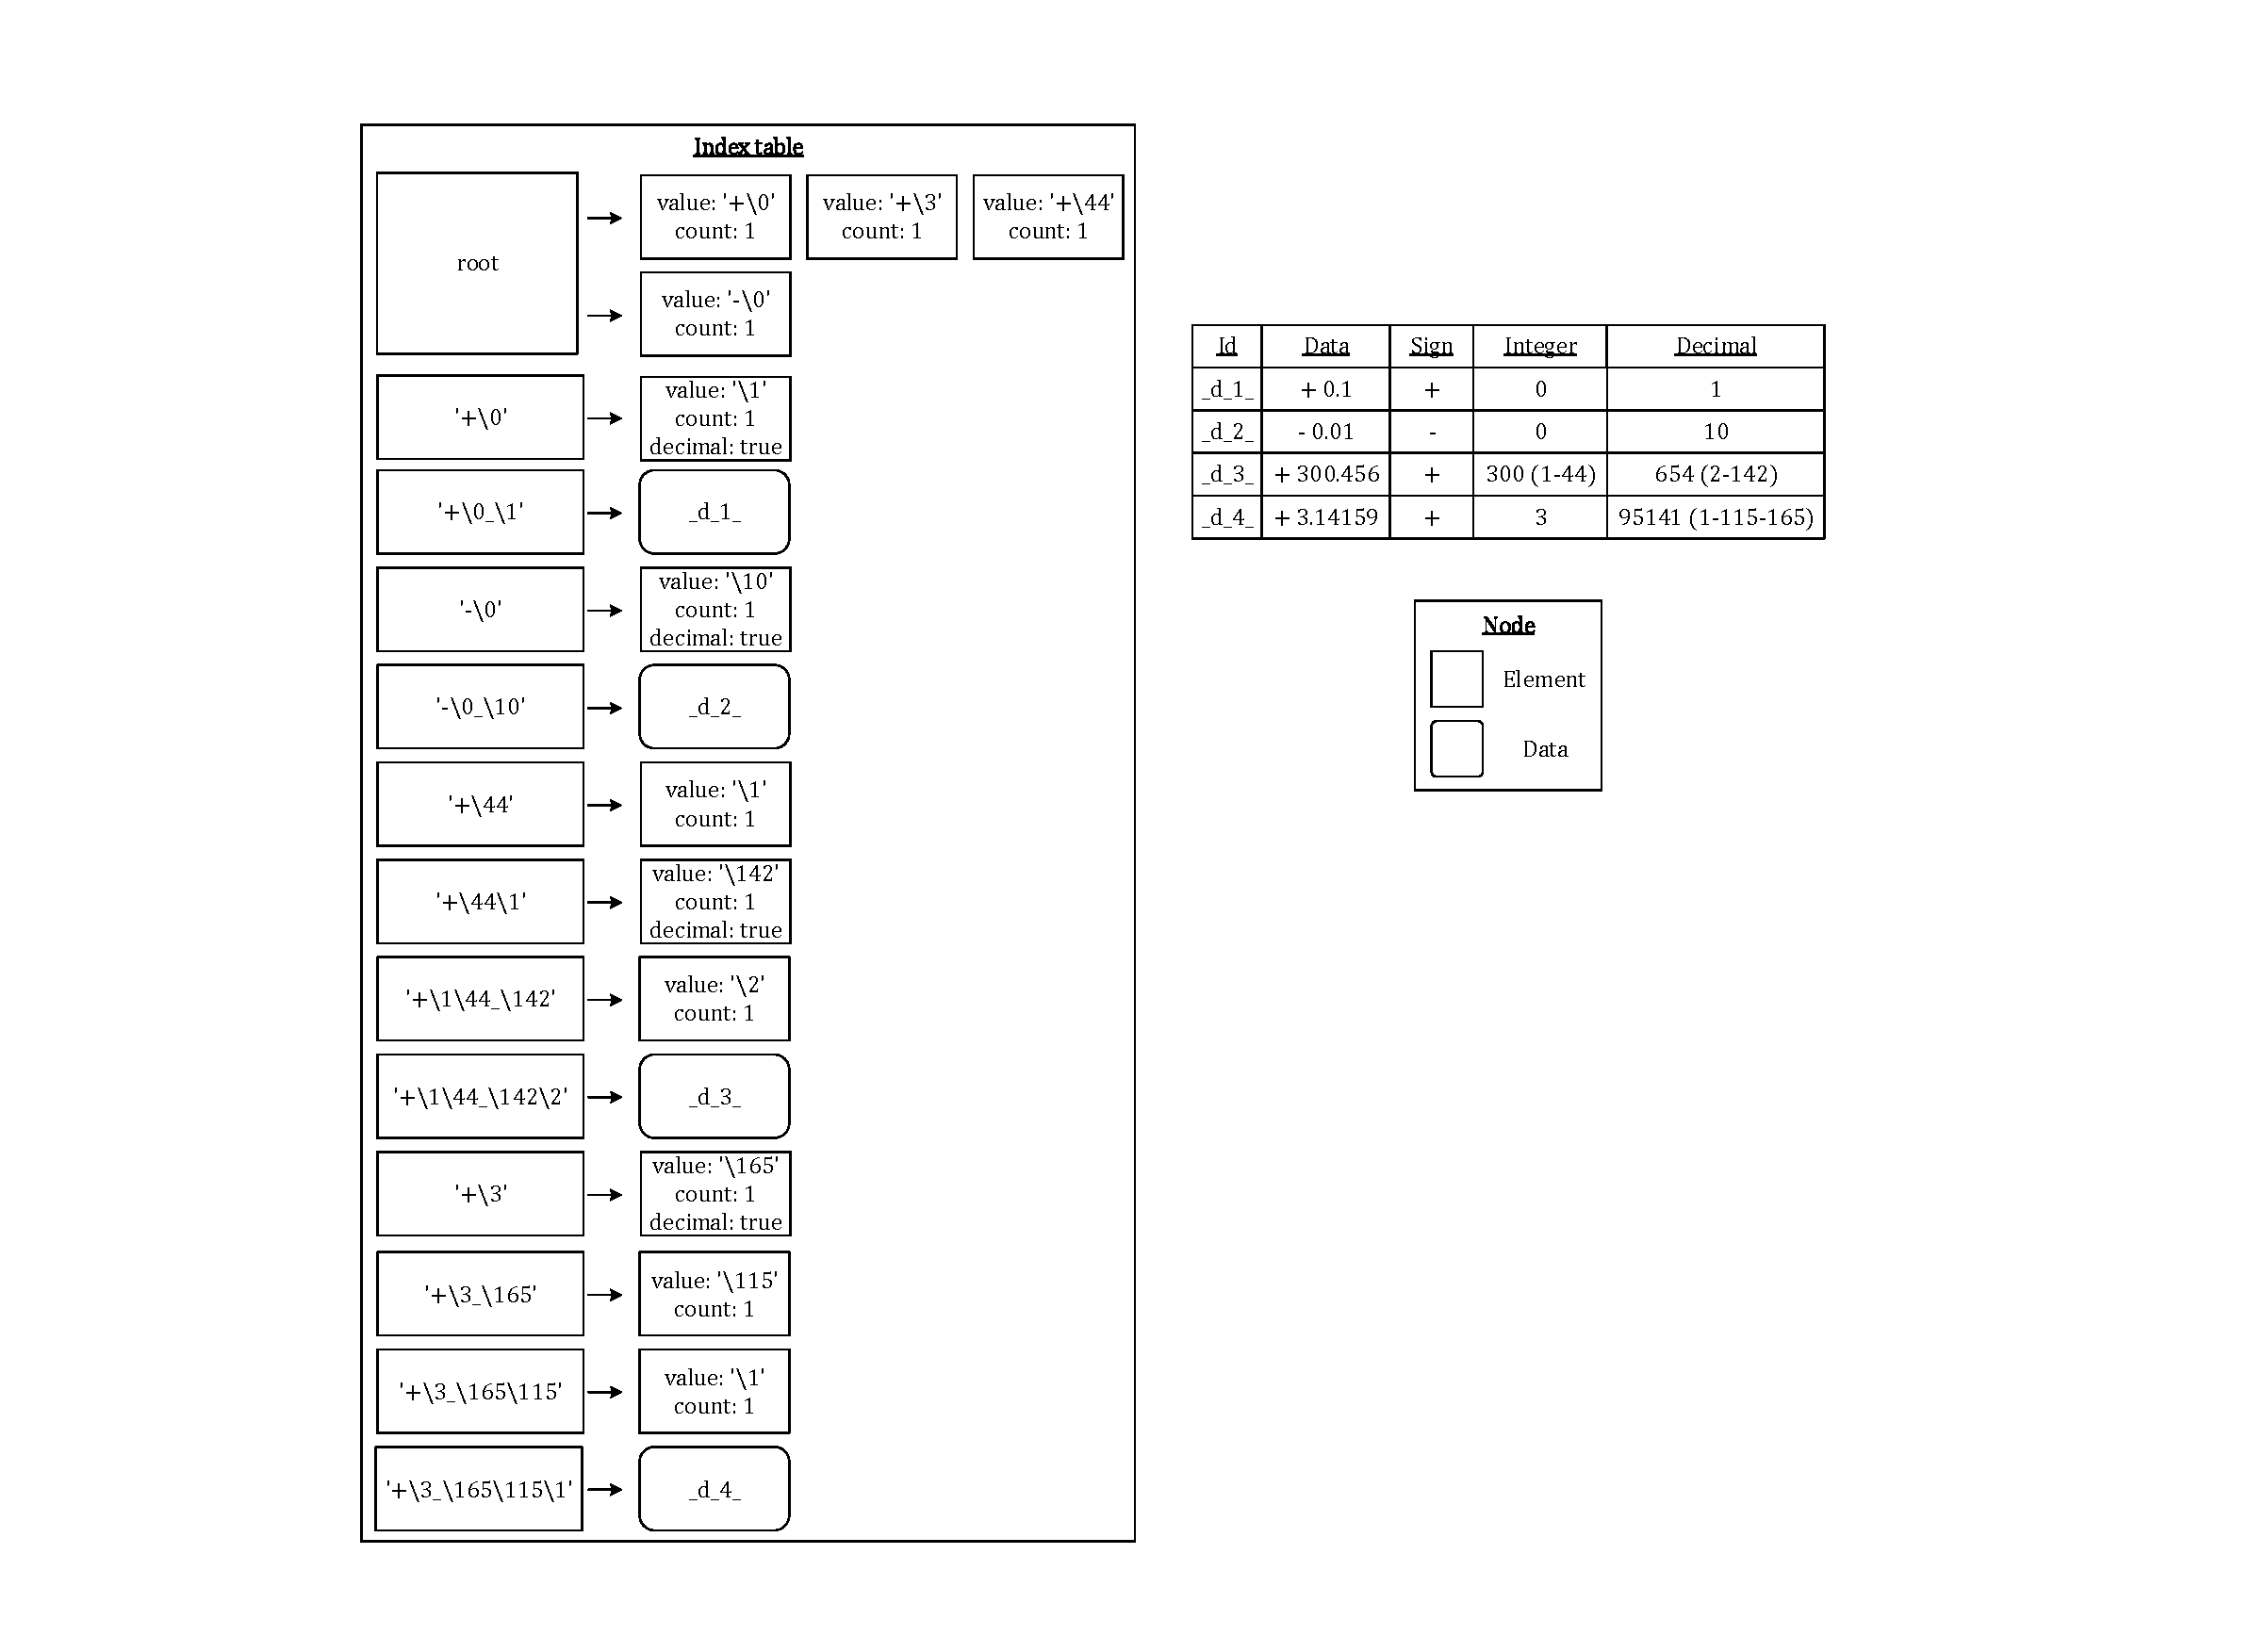
\includegraphics[width=0.8\textwidth]{./algorithm/real/pic/insertion/example_v4.pdf}
\caption{The table after inserted $\pi (3.14159)$.}
\label{fig:algorithm:real:insertion:example}
\end{figure}

Figure \ref{fig:algorithm:real:insertion:example} shows that the $\pi (+3.14159)$ is store the value by its \textit{"Sign"} $(+)$, \textit{"Integer"} $(3)$ and \textit{"Decimal"} $(95141)$.

The \textit{"Sign"} is pointing the last byte of the \textit{"Integer"}, the reason of point to the last byte is because of the dynamic length of \textit{REAL}, also assume the the byte of the data is longer than the input byte length:

\begin{enumerate}

\item  If the \textit{"Sign"} is pointing the first byte, then when we search the result for the input, this may need to compare more byte or we need to get the whole \textit{"Integer"} in the worst case to sure that this value is suitable or not to the input.

\item If \textit{"Sign"} is pointing the last byte, then we just need to compare few bytes or the same byte length of the input that we can immediately to know that is a result or not. So this indexing can speed up the searching.

\end{enumerate}

Time complexity should be $O(b!)$ which domain as $O(b)$, and $b$ is the length of the byte needed where $b = 4$ in this case.



% Deletion section
\subsubsection{Deletion}

Deletion is just do the opposite insertion to remove the byte and decrease the count. So time complexity be $O(b)$.



% Modification section
\subsubsection{Modification}

The modify flow are similar as \textit{INTEGER} type, remove the key which don't needed and add the count if the byte is the same. So follow the example in figure \ref{fig:algorithm:real:insertion:example} and then modify -$0.01$ to +$0.0$ (because zero don't contain positive or negative sign, so using positive sign should be fine), the table will look like figure \ref{fig:algorithm:real:modification:example} and the time complexity be $O(b)$.

\begin{figure}[h]
\centering
%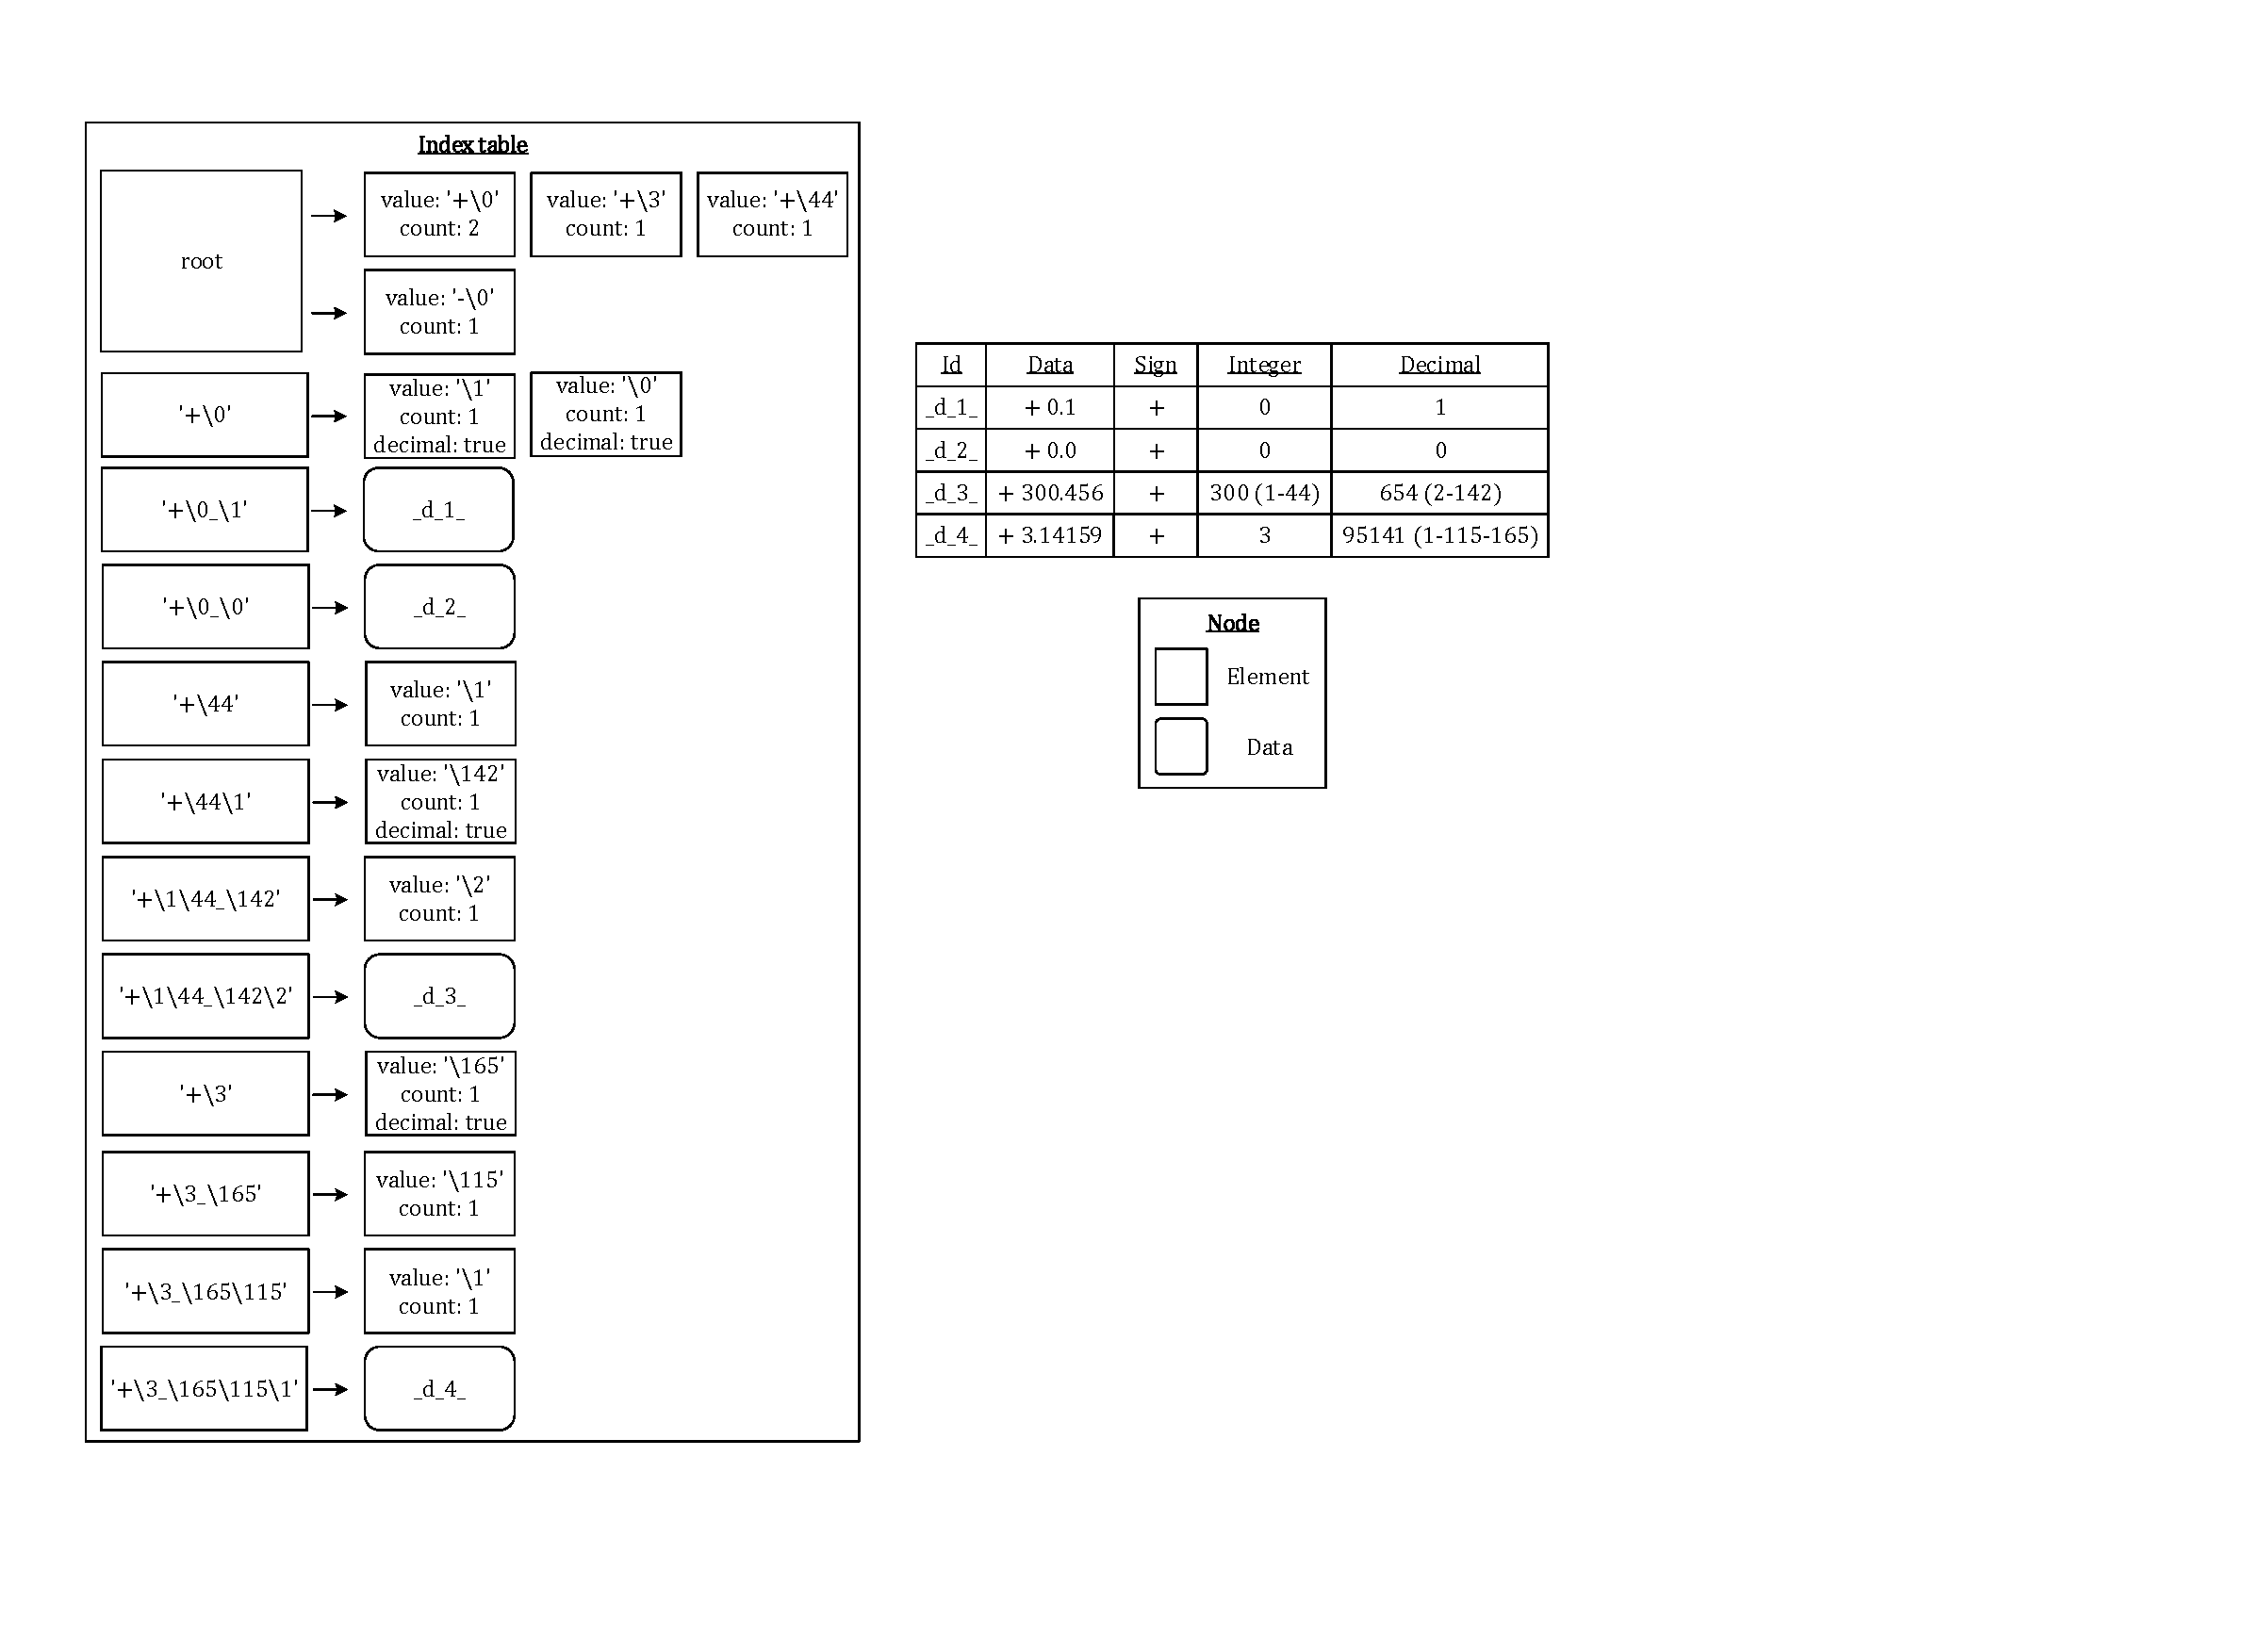
\includegraphics[scale=0.5]{./algorithm/real/pic/modification/example_v4.pdf}
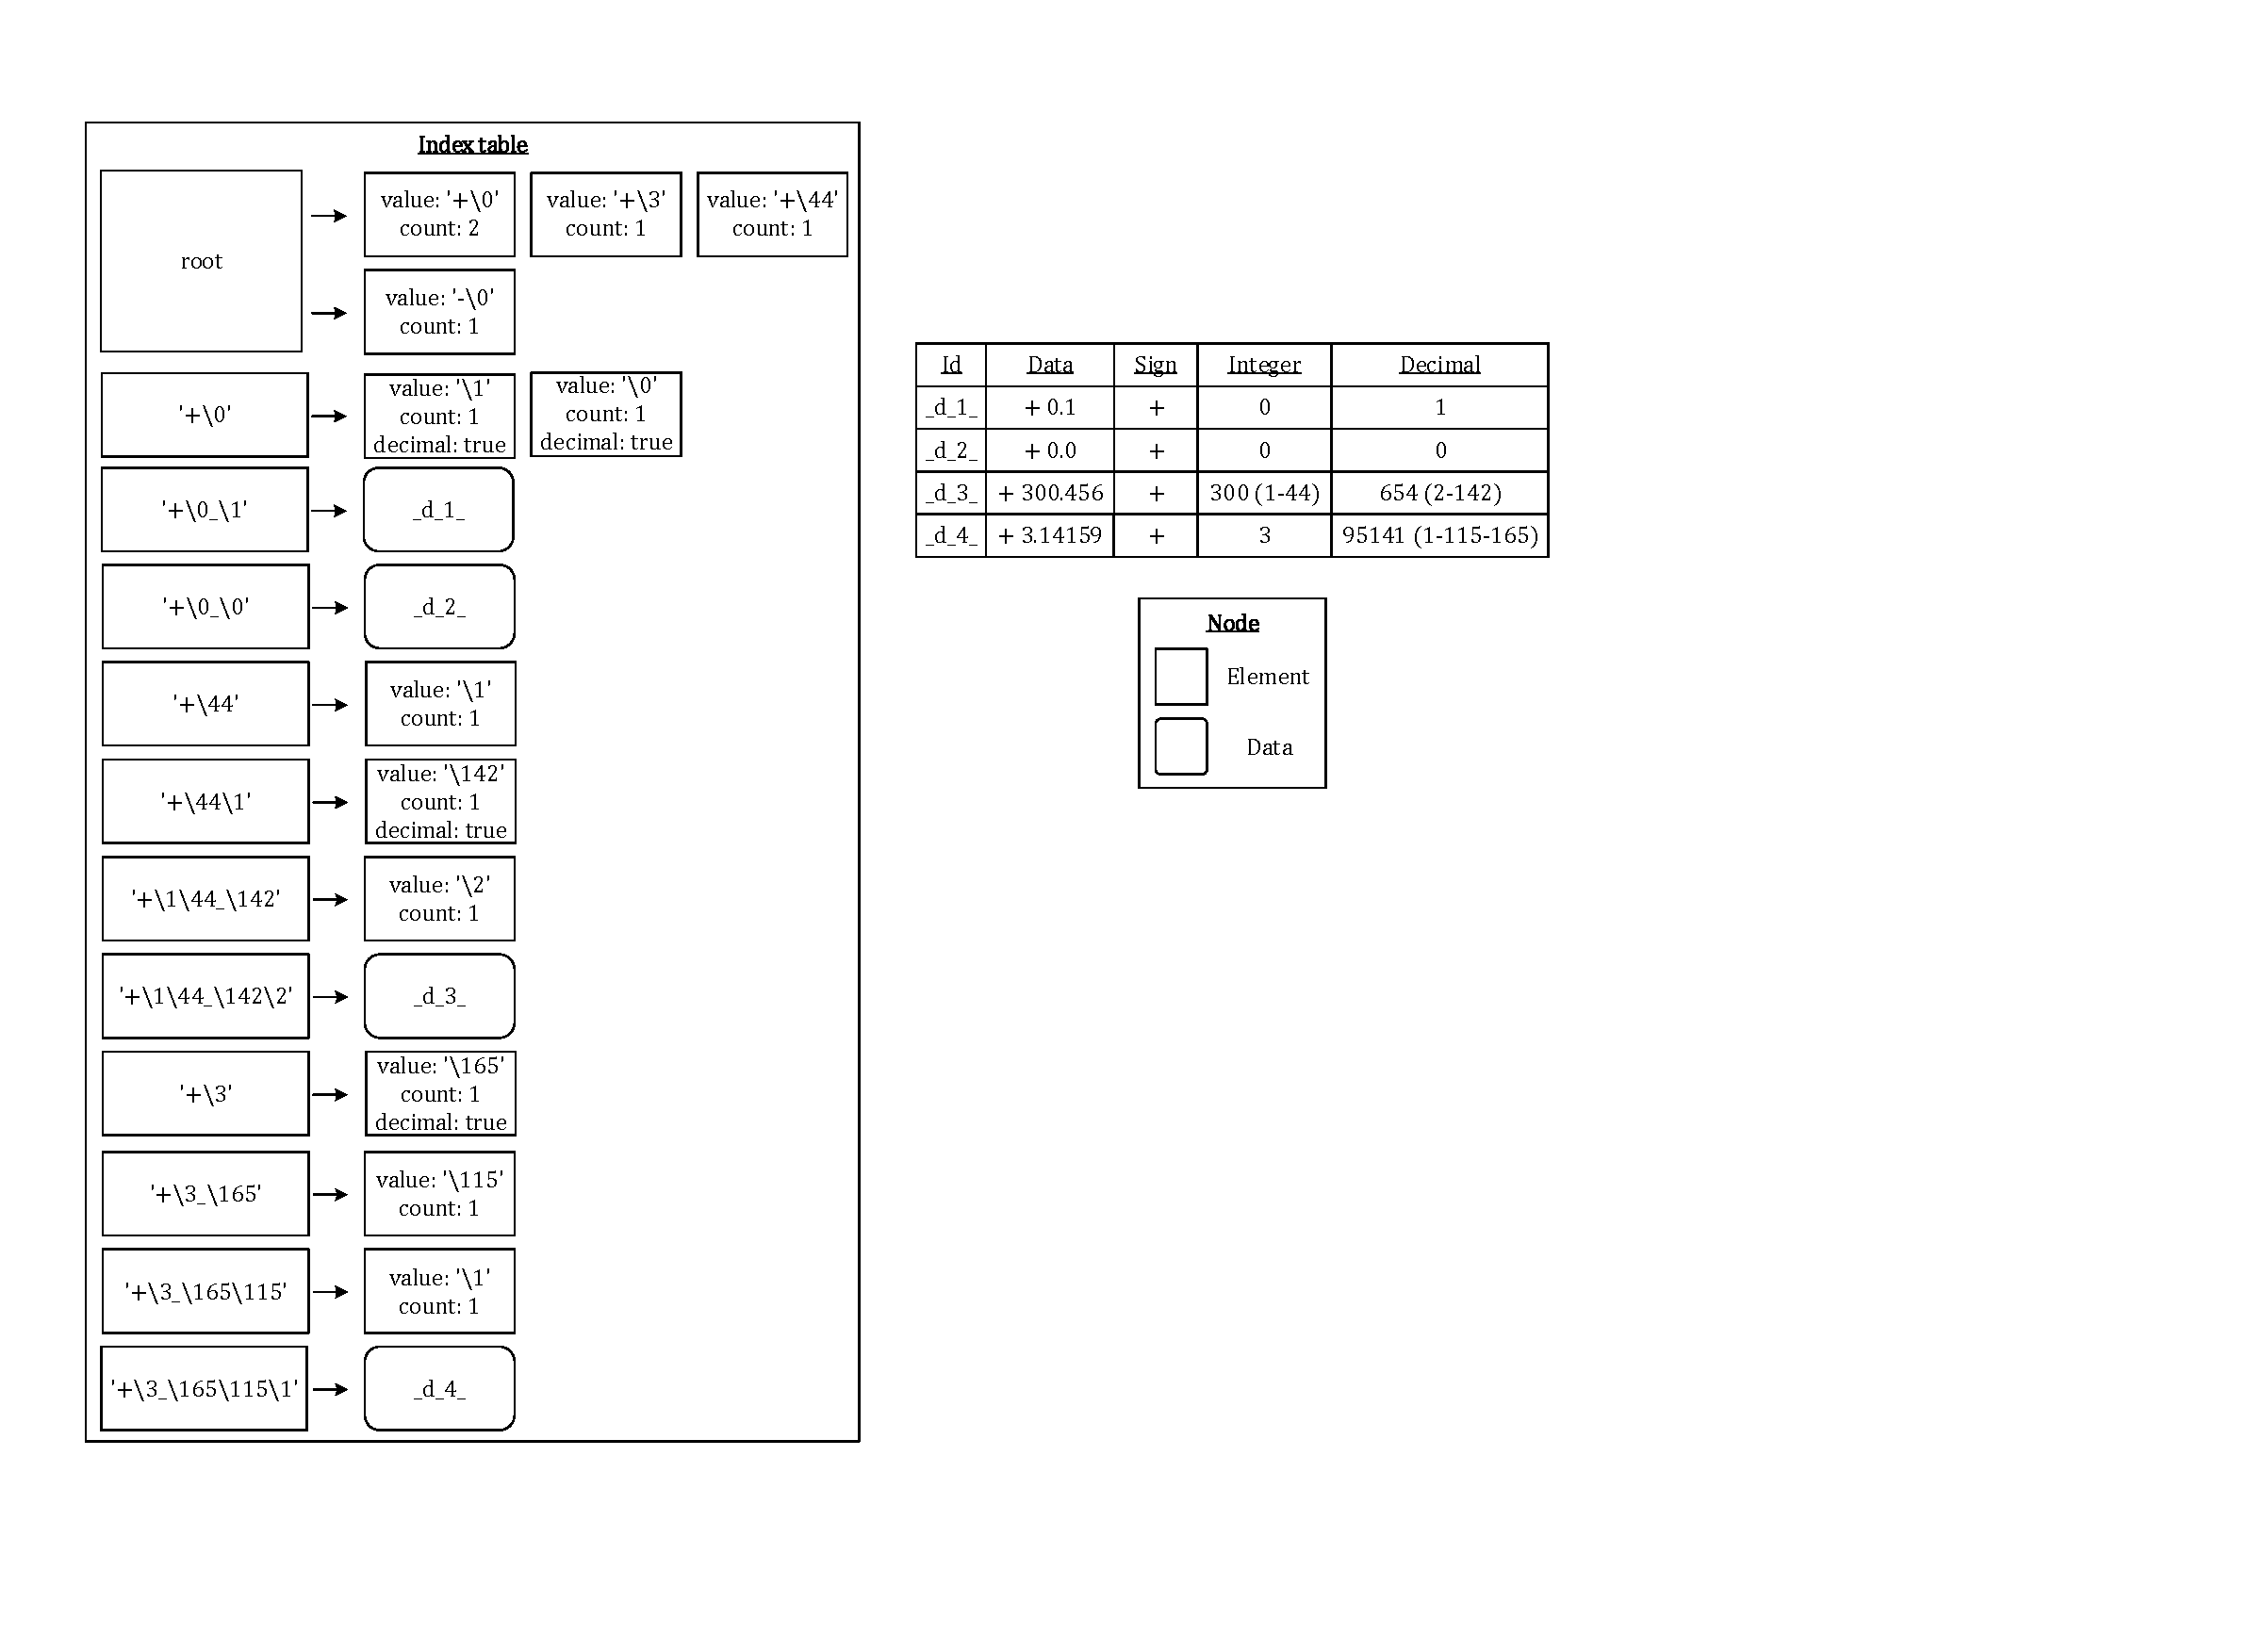
\includegraphics[width=0.8\textwidth]{./algorithm/real/pic/modification/example_v4.pdf}
\caption{The table after modified the value.}
\label{fig:algorithm:real:modification:example}
\end{figure}



% Selection section
\subsubsection{Selection}

The follow operations will use figure \ref{fig:algorithm:real:modification:example} as the example.

% Selection section enumerate
\begin{enumerate}

% --------------------------------------------------------

% Equal
\item \textbf{Equal}

If search \textit{0.0}, then convert it into three part: \textit{"Sign"}, \textit{"Integer"} and \textit{"Decimal"}, which means $'$+$\backslash0\backslash\_\backslash0'$ and use this as key to get the result, this should take $O(1)$.

% --------------------------------------------------------

% Not equal
\item \textbf{Not equal}

If searching the result which is not equal \textit{0.0}, strat of convert it into key, then start from root, then recursively to find the data nodes and only skip the key of input. This operation should take $O(b)$.

% --------------------------------------------------------

% Less than
\item \textbf{Less than}

When comparing the \emph{"Less than"} or \emph{"Greater}, the flow is way different as the other because of the dynamic byte design.

For example searching \textit{300.0} in table, then convert into string $'$+$\backslash44\backslash1\_\backslash0'$ which the length of \textit{"Integer"} is \textit{2} and \textit{1} for \textit{"Decimal"} that the two value is use to let the compare function know how deep of the byte need to search.

% Less than section enumerate
\begin{enumerate}

% Input value is a negative value
\item \textbf{Input value is a negative value}

\begin{enumerate}

\item Start from root and only get the nodes which the \textit{"Sign"} are \textit{'-'}.

\item When searching \textit{"Integer"} part, recursively to search the element node contain \textit{decimal} with the length is \textit{"longer than or equal to"} to the \textit{"Integer"} length of input (in this case is \textit{2}). Then only remain the nodes that the value of \textit{"Integer"} is \textit{"larger than or equal to"} the value in \textit{"Integer"} part of input.

\item Searching in \textit{"Decimal"} part:
\begin{enumerate}

\item If the length of \textit{"Integer"} part is \textit{"longer than"} the input, then get all the data nodes.

\item If the length of \textit{"Integer"} part is \textit{"equal to"} the input, then recursively and only get the element nodes that the length is \textit{"greater than or equal to"} the length of \textit{"Decimal"} of input. And check the value of \textit{"Decimal"} is \textit{"larger than"} the value in \textit{"Decimal"} part of input.
\end{enumerate}

\end{enumerate}

% Input value is a positive value
\item \textbf{Input value is a positive value}

\begin{enumerate}

\item Get all the data nodes start from root which the \textit{"Sign"} are \textit{'-'}.

\item Next start from root and get the nodes which the \textit{"Sign"} are \textit{'+'}.

\item When searching \textit{"Integer"} part, recursively to search the element node contain \textit{decimal} with the length is \textit{"shorter than or equal to"} to the \textit{"Integer"} length of input (in this case is \textit{2}). Then only remain the nodes that the value of \textit{"Integer"} is \textit{"smaller than or equal to"} than the value in \textit{"Integer"} part of input.

\item Searching in \textit{"Decimal"} part:
\begin{enumerate}

\item If the length of \textit{"Integer"} part is \textit{"shorter than"} the input, then get all the data nodes.

\item If the length of \textit{"Integer"} part is \textit{"equal to"} the input, then recursively and only get the element nodes that the length is \textit{"shorter than or equal to"} the length of \textit{"Decimal"} of input. And check the value of \textit{"Decimal"} is \textit{"smaller than"} the value in \textit{"Decimal"} part of input.
\end{enumerate}

\end{enumerate}

% Input value is equal to 0.0
\item \textbf{Input value is equal to \textit{0.0}}

Get all the data nodes start from root which the \textit{"Sign"} are \textit{'-'}.

% End Less than section enumerate
\end{enumerate}

The \emph{"Less than or equal to"} comparison is just do the \emph{"Less than"} and \emph{"Equal"} operation and then combine both result for ouput. The time complexity is $O(b)$ for both operation.

% --------------------------------------------------------

% Greater than
\item \textbf{Greater than}

This comparison flow is similar as \emph{"Less than"}.

% Greater than section enumerate
\begin{enumerate}

% Input value is a negative value
\item \textbf{Input value is a negative value}

\begin{enumerate}

\item Get all the data nodes start from root which the \textit{"Sign"} are \textit{'+'}.

\item Next start from root and get the nodes which the \textit{"Sign"} are \textit{'-'}.

\item When searching \textit{"Integer"} part, recursively to search the element node contain \textit{decimal} with the length is \textit{"shorter than or equal to"} to the \textit{"Integer"} length of input. Then only remain the nodes that the value of \textit{"Integer"} is \textit{"larger than or equal to"} than the value in \textit{"Integer"} part of input.

\item Searching in \textit{"Decimal"} part:
\begin{enumerate}

\item If the length of \textit{"Integer"} part is \textit{"shorter than"} the input, then get all the data nodes.

\item If the length of \textit{"Integer"} part is \textit{"equal to"} the input, then recursively and only get the element nodes that the length is \textit{"shorter than or equal to"} the length of \textit{"Decimal"} of input. And check the value of \textit{"Decimal"} is \textit{"larger than"} the value in \textit{"Decimal"} part of input.
\end{enumerate}

\end{enumerate}

% Input value is a positive value
\item \textbf{Input value is a positive value}

\begin{enumerate}

\item Start from root and only get the nodes which the \textit{"Sign"} are \textit{'+'}.

\item When searching \textit{"Integer"} part, recursively to search the element node contain \textit{decimal} with the length is \textit{"longer than or equal to"} to the \textit{"Integer"} length of input. Then only remain the nodes that the value of \textit{"Integer"} is \textit{"larger than or equal to"} the value in \textit{"Integer"} part of input.

\item Searching in \textit{"Decimal"} part:
\begin{enumerate}

\item If the length of \textit{"Integer"} part is \textit{"longer than"} the input, then get all the data nodes.

\item If the length of \textit{"Integer"} part is \textit{"equal to"} the input, then recursively and only get the element nodes that the length is \textit{"greater than or equal to"} the length of \textit{"Decimal"} of input. And check the value of \textit{"Decimal"} is \textit{"larger than"} the value in \textit{"Decimal"} part of input.
\end{enumerate}

\end{enumerate}

% Input value is equal to 0.0
\item \textbf{Input value is equal to \textit{0.0}}

Get all the data nodes start from root which the \textit{"Sign"} are \textit{'+'} but skip the key of \textit{+0.0}.

% End Greater than section enumerate
\end{enumerate}

The \emph{"Greater than or equal to"} comparison is just do the \emph{"Greater than"} and \emph{"Equal"} operation and then combine both result for ouput. The time complexity is $O(b)$ for both operation.

% --------------------------------------------------------

% Between
\item \textbf{Between}

The \textit{between} operation of \textit{REAL} is as same as the \textit{between} operation of the \textit{signed INTEGER}, so skip the description of this part. The time complexity is $O(b)$.

% --------------------------------------------------------

\end{enumerate}


% Summary section
\subsubsection{Summary}

Table \ref{table:algorithm:real:summary:time_complexity} is a summary the time complexity of each opration in \textit{REAL} type.

\begin{table}[h]
\centering
\caption{Time complexity for \textit{REAL} type.}
\label{table:algorithm:real:summary:time_complexity}
\begin{tabular}{|c|c|}

\hline
\multicolumn{1}{|c|}{Operation} &
\multicolumn{1}{c|}{\tabincell{c}{
Time complexity \\ ($b$: The byte length of data)
}} \\

\hline
\multicolumn{1}{|c|}{Insert} &
\multicolumn{1}{c|}{$O(b)$} \\

\hline
\multicolumn{1}{|c|}{Modify} &
\multicolumn{1}{c|}{$O(b)$} \\

\hline
\multicolumn{1}{|c|}{Delete} &
\multicolumn{1}{c|}{$O(b)$} \\

\hline
\multicolumn{1}{|c|}{Equal} &
\multicolumn{1}{c|}{$O(1)$} \\

\hline
\multicolumn{1}{|c|}{\tabincell{c}{Equal (muti-value)}} &
\multicolumn{1}{c|}{$O(1)$} \\

\hline
\multicolumn{1}{|c|}{Not equal} &
\multicolumn{1}{c|}{$O(b)$} \\

\hline
\multicolumn{1}{|c|}{\tabincell{c}{Not equal (muti-value)}} &
\multicolumn{1}{c|}{$O(b)$} \\

\hline
\multicolumn{1}{|c|}{Less than} &
\multicolumn{1}{c|}{$O(b)$} \\

\hline
\multicolumn{1}{|c|}{Less than or equal} &
\multicolumn{1}{c|}{$O(b)$} \\

\hline
\multicolumn{1}{|c|}{Greater than} &
\multicolumn{1}{c|}{$O(b)$} \\

\hline
\multicolumn{1}{|c|}{Greater than or equal} &
\multicolumn{1}{c|}{$O(b)$} \\

\hline
\multicolumn{1}{|c|}{Between} &
\multicolumn{1}{c|}{$O(b)$} \\

\hline
\end{tabular}
\end{table}

\textit{REAL} is target for the data type of \textit{"long double"}, the only disadvantage that it will need more byte to store the value compare with \textit{"long double"}. From table \ref{table:algorithm:real:design_data_type} shows that the \textit{"float"} can store the range beyond the \textit{"Bigint"}, so that this mean it will need many \textit{"Bigint"} to store the value in \textit{"long double"}.

\begin{table}[h]
\centering
\caption{Information about data type.}
\label{table:algorithm:real:design_data_type}
\begin{tabular}{|c|c|c|}

\hline
\multicolumn{1}{|c|}{Data type} &
\multicolumn{1}{c|}{Range} &
\multicolumn{1}{c|}{Bytes} \\

\hline
\multicolumn{1}{|c|}{float} &
\multicolumn{1}{c|}{$3.40282e^{+038}$ $\thicksim$ $1.17549e^{-038}$} &
\multicolumn{1}{c|}{4} \\

\hline
\multicolumn{1}{|c|}{double} &
\multicolumn{1}{c|}{$1.79769e^{+308}$ $\thicksim$ $2.22507e^{-308}$} &
\multicolumn{1}{c|}{8} \\

\hline
\multicolumn{1}{|c|}{long double} &
\multicolumn{1}{c|}{$1.18973e^{+4932}$ $\thicksim$ $3.3621e^{-4932}$} &
\multicolumn{1}{c|}{16} \\

\hline
\multicolumn{1}{|c|}{unsigned int} &
\multicolumn{1}{c|}{0 $\thicksim$ 4294697295} &
\multicolumn{1}{c|}{4} \\

\hline
\multicolumn{1}{|c|}{\tabincell{c}{
unsigned long long int \\ (Bigint)
}} &
\multicolumn{1}{c|}{0 $\thicksim$ 18446744073709551615} &
\multicolumn{1}{c|}{8} \\

\hline
\end{tabular}
\end{table}

But the advantage of \textit{REAL} that it can store the value with 100\% accuracy, also provide comparison and sorting, and it can store limitless data range. So no matter the basic use of the floating point such as Financial or Basic operations, these usage is hard to use more than five digital in \textit{"Decimal"} part. Also \textit{REAL} can store special data like science data such as the value in physics, this kind of usage may need to use up to thousand digital in \textit{"Decimal"} part, this is a normal range of \textit{"long double"}.\\



\clearpage



% BLOB section
\subsection{BLOB type}

Rather than the other data type, BLOB type is much more similar as the normal \textit{put()} because it don't do any indexing. So that it can't do any selection and comparison so that it need to work with other data type, there is a example show in figure \ref{fig:table_design:example} in section \ref{sec:table_design}.


\clearpage

% Summary and case study section
\subsection{Summary and case study}

Table \ref{table:algorithm:summary:time_complexity} is a summarization and the time complexity of each operation.\\

% Time complexity table
\begin{table}[h]
\centering
\caption{Time complexity of all data type ($b$: The byte length of data)}
\label{table:algorithm:summary:time_complexity}
\begin{tabular}{|c|c|c|c|c|c|}

%\hline
%\multicolumn{6}{|c|}{\tabincell{c}{
%Time complexity \\ ($b$: The byte length of data)
%}} \\

\hline
\multicolumn{1}{|c|}{Operation} &
\multicolumn{1}{c|}{BLOB} &
\multicolumn{1}{c|}{STRING} &
\multicolumn{1}{c|}{BOOLEAN} &
\multicolumn{1}{c|}{INTEGER} &
\multicolumn{1}{c|}{REAL} \\

\hline
\multicolumn{1}{|c|}{Insertion} &
\multicolumn{1}{c|}{X} &
\multicolumn{1}{c|}{$O(b)$} &
\multicolumn{1}{c|}{$O(1)$} &
\multicolumn{1}{c|}{$O(b)$} &
\multicolumn{1}{c|}{$O(b)$} \\

\hline
\multicolumn{1}{|c|}{Modification} &
\multicolumn{1}{c|}{X} &
\multicolumn{1}{c|}{$O(b)$} &
\multicolumn{1}{c|}{$O(1)$} &
\multicolumn{1}{c|}{$O(b)$} &
\multicolumn{1}{c|}{$O(b)$} \\

\hline
\multicolumn{1}{|c|}{Deletion} &
\multicolumn{1}{c|}{X} &
\multicolumn{1}{c|}{$O(b)$} &
\multicolumn{1}{c|}{$O(1)$} &
\multicolumn{1}{c|}{$O(b)$} &
\multicolumn{1}{c|}{$O(b)$} \\

\hline
\multicolumn{1}{|c|}{Equal} &
\multicolumn{1}{c|}{X} &
\multicolumn{1}{c|}{\tabincell{c}{$O(1)$\\(Exact matching)}} &
\multicolumn{1}{c|}{$O(1)$} &
\multicolumn{1}{c|}{$O(1)$} &
\multicolumn{1}{c|}{$O(1)$} \\

\hline
\multicolumn{1}{|c|}{\tabincell{c}{Equal (muti-value)}} &
\multicolumn{1}{c|}{X} &
\multicolumn{1}{c|}{\tabincell{c}{$O(1)$\\(Exact matching)}} &
\multicolumn{1}{c|}{X} &
\multicolumn{1}{c|}{$O(1)$} &
\multicolumn{1}{c|}{$O(1)$} \\

\hline
\multicolumn{1}{|c|}{Not equal} &
\multicolumn{1}{c|}{X} &
\multicolumn{1}{c|}{$O(b)$} &
\multicolumn{1}{c|}{$O(1)$} &
\multicolumn{1}{c|}{$O(b)$} &
\multicolumn{1}{c|}{$O(b)$} \\

\hline
\multicolumn{1}{|c|}{\tabincell{c}{Not equal (muti-value)}} &
\multicolumn{1}{c|}{X} &
\multicolumn{1}{c|}{$O(b)$} &
\multicolumn{1}{c|}{X} &
\multicolumn{1}{c|}{$O(b)$} &
\multicolumn{1}{c|}{$O(b)$} \\

\hline
\multicolumn{1}{|c|}{Less than} &
\multicolumn{1}{c|}{X} &
\multicolumn{1}{c|}{X} &
\multicolumn{1}{c|}{X} &
\multicolumn{1}{c|}{$O(b)$} &
\multicolumn{1}{c|}{$O(b)$} \\

\hline
\multicolumn{1}{|c|}{Less than or equal} &
\multicolumn{1}{c|}{X} &
\multicolumn{1}{c|}{X} &
\multicolumn{1}{c|}{X} &
\multicolumn{1}{c|}{$O(b)$} &
\multicolumn{1}{c|}{$O(b)$} \\

\hline
\multicolumn{1}{|c|}{Greater than} &
\multicolumn{1}{c|}{X} &
\multicolumn{1}{c|}{X} &
\multicolumn{1}{c|}{X} &
\multicolumn{1}{c|}{$O(b)$} &
\multicolumn{1}{c|}{$O(b)$} \\

\hline
\multicolumn{1}{|c|}{Greater than or equal} &
\multicolumn{1}{c|}{X} &
\multicolumn{1}{c|}{X} &
\multicolumn{1}{c|}{X} &
\multicolumn{1}{c|}{$O(b)$} &
\multicolumn{1}{c|}{$O(b)$} \\

\hline
\multicolumn{1}{|c|}{Between} &
\multicolumn{1}{c|}{X} &
\multicolumn{1}{c|}{X} &
\multicolumn{1}{c|}{X} &
\multicolumn{1}{c|}{$O(b)$} &
\multicolumn{1}{c|}{$O(b)$} \\

\hline
\multicolumn{1}{|c|}{\tabincell{c}{Search \\ (Exact matching)}} &
\multicolumn{1}{c|}{X} &
\multicolumn{1}{c|}{$O(1)$} &
\multicolumn{1}{c|}{X} &
\multicolumn{1}{c|}{X} &
\multicolumn{1}{c|}{X} \\

\hline
\multicolumn{1}{|c|}{\tabincell{c}{Search \\ (Prefix matching)}} &
\multicolumn{1}{c|}{X} &
\multicolumn{1}{c|}{$O(b)$} &
\multicolumn{1}{c|}{X} &
\multicolumn{1}{c|}{X} &
\multicolumn{1}{c|}{X} \\

\hline
\multicolumn{1}{|c|}{\tabincell{c}{Search \\ (Suffix matching)}} &
\multicolumn{1}{c|}{X} &
\multicolumn{1}{c|}{$O(b)$} &
\multicolumn{1}{c|}{X} &
\multicolumn{1}{c|}{X} &
\multicolumn{1}{c|}{X} \\

\hline
\multicolumn{1}{|c|}{\tabincell{c}{Search \\ (Partial matching)}} &
\multicolumn{1}{c|}{X} &
\multicolumn{1}{c|}{$O(b)$} &
\multicolumn{1}{c|}{X} &
\multicolumn{1}{c|}{X} &
\multicolumn{1}{c|}{X} \\

\hline
\end{tabular}
\end{table}

% Capacity table
\begin{table}[h]
\centering
\caption{Capacity needed of with all type (Unit: byte)}
\label{table:algorithm:summary:capacity}
\begin{tabular}{|c|c|c|c|c|c|}

\hline
\multicolumn{1}{|c|}{Type} &
\multicolumn{1}{c|}{BLOB} &
\multicolumn{1}{c|}{STRING} &
\multicolumn{1}{c|}{BOOLEAN} &
\multicolumn{1}{c|}{INTEGER} &
\multicolumn{1}{c|}{REAL} \\

\hline
\multicolumn{1}{|c|}{byte length} &
\multicolumn{1}{c|}{$n$} &
\multicolumn{1}{c|}{$n$} &
\multicolumn{1}{c|}{$n$} &
\multicolumn{1}{c|}{$8$} &
\multicolumn{1}{c|}
{\tabincell{c}{
$1 + n + m$ \\ ($n$ is byte length of \textit{"Integer"} part and \\
$m$ is byte length of \textit{"Decimal"} part)
}} \\

\hline
\multicolumn{1}{|c|}{index size} &
\multicolumn{1}{c|}{$0$} &
\multicolumn{1}{c|}{$$} &
\multicolumn{1}{c|}
{\tabincell{c}{
$2$ \\ (\textit{'+'} and \textit{'-'})
}} &
\multicolumn{1}{c|}{$$} &
\multicolumn{1}{c|}{$$} \\

\hline
\multicolumn{1}{|c|}{Total size} &
\multicolumn{1}{c|}{$n$} &
\multicolumn{1}{c|}{$$} &
\multicolumn{1}{c|}{$n + 2$} &
\multicolumn{1}{c|}{$$} &
\multicolumn{1}{c|}{$$} \\

\hline
\end{tabular}
\end{table}


\clearpage

% ------------------------------------------------
% End of page
% ------------------------------------------------


% Performance chapter
%% ------------------------------------------------
% Page start
% ------------------------------------------------
\chapter{Performance Evaluation}
\label{chapter:performance-evaluation}

\baselineskip=26pt
\thispagestyle{empty}
% ------------------------------------------------

% Time evaluation section
\subsection{Time evaluation}

% Setup section
\subsubsection{Setup}

To measure the performance of Li's Hash by measuring the time of each data type (except BLOB) and operation and compare with SQLite \cite{web:sqlite:home-page}, MariaDB \cite{web:mariadb:home-page} and PostgreSQL \cite{web:postgresql:home-page} by using single table in memory to remove any possible I/O delay.\\

There is no SQL parser for Li's Hash which may this test un-fair, but a SQL parser can't too slow because it is one of core part for a SQL database. We observe the timing of SQLite and it take < 0.001 ms per SQL on our platform. So it seem that the time is too small that can be ignore.\\

Also, because normally the real hash table will use the index as a pointer, but the problem is that kind of hash table need to use a static array, but a dynamic hash table that even the std::map in standard C++ library, it still need to use the $\log(n)$ like the other B+ tree does.\\

So if still use these kind library as our back-end storage to do the testing which will not see the improvement of our design, so that we implemented our own back-end storage based on Radix tree \cite{web:wiki:radix-tree} and it work similar as the design of the Linux kernel does \cite{web:linux-kernel:radix-tree}.\\

%\begin{figure}[h]
%\centering
%\includegraphics[scale=0.5]{./performance/pic/a.png}
%\caption{The Radix tree design.}
%\label{fig:performance:}
%\end{figure}

%Figure \cite{fig:performance:} is our design look like, we hash the key become a number (Same as the ring design in Dynamo \cite{paper:amazon-dynamo-1}), next convert the number into byte array which that the index will become its' depth and the value of the byte will be as its' index number for moving to the downward, until found the leaf which is the data storage.\\

%Collision is very easy happen in hash function, we can do two way to slove it in our tree design:

%\begin{enumerate}

%\item \textbf{Increase the depth of tree}\\
%Increase the byte length of the hash function output, which means incease the depth of tree.

%\item \textbf{Multi-level tree}\\
%Our Radix tree can become a multi-level tree, will mean the leaf can become the root of the next level tree.

%The reason of this design is a single hash function still can cause a very small collision, so if using a tree that build from multi-hash function that should highly decrease the collision probelm.

%\end{enumerate}

% Testing section
\subsection{Testing}

We use the default configure for SQLite base on assume the user is new for it, then he/she will only care the performance in the default, also the default is set by the offical that what they think is the best, so this can be as a baseline of the database.\\

%We use 100,000 rows (keys) for test the performance on our platform. The reason is because we tested up to 500,000 and found out when SQLite enabled the indexing, the average time per SQL seem very static, so testing more rows seem don't prodive any useful information.

% Hardware table

\begin{table}[ht]
\centering
\label{table:performance:testing-platform}
\begin{tabular}{|c|c|}

\hline
\multicolumn{1}{|r|}{CPU:} &
\multicolumn{1}{c|}{Intel Xeon E5-2620} \\

\hline
\multicolumn{1}{|r|}{RAM:} &
\multicolumn{1}{c|}{180 GB} \\

\hline
\multicolumn{1}{|r|}{OS:} &
\multicolumn{1}{c|}{Ubuntu 12.04.4} \\

\hline
\multicolumn{1}{|r|}{Kernel:} &
\multicolumn{1}{c|}{3.11.0-15-generic} \\

\hline
\multicolumn{1}{|r|}{GCC version:} &
\multicolumn{1}{c|}{4.6.3} \\

\hline
\multicolumn{1}{|r|}{SQLite version:} &
\multicolumn{1}{c|}{3.8.1} \\

\hline
\end{tabular}
\end{table}



\clearpage

% ----------------------------------------------------------

\begin{enumerate}


%In this layer, we test the baseline of all databases without using the index, but without index the Li's Hash can't do query as a normal non-relational database. So we only test the performance of the back-end database by only use the basic put(), get() for all data type in Li's Hash. Also only use normal SELECT, INSERT in relational database without enable index.\\

% Database layer section
\item \textbf{Database layer}

In this layer, we test the baseline of both databases without using the index, but without index the Li's Hash can't do query as a normal non-relational data-base. So we only test the performance of the back-end data-base by using the basic \textit{put()}, \textit{get()} for all data type in Li's Hash. Also only use normal SELECT, INSERT in relational database without enable index. We use the code in table \ref{table:performance:database-layer:code-example} to do this test.\\

% Database layer test table 

% Database layer test
\begin{table*}
\centering
\caption{Example code that to test STRING type in \textit{Database layer}}
\label{table:performance:database-layer:code-example}
\begin{tabular}{|c|c|c|}

\hline
\multicolumn{1}{|c|}{} &
\multicolumn{1}{c|}{\textbf{Li's Hash}} &
\multicolumn{1}{c|}{\textbf{Relational database}} \\

\hline
\multicolumn{1}{|c|}{Create table} &
\multicolumn{1}{c|}
{\tabincell{c}{
X \\ (Key-value store don't need table)
}} &
\multicolumn{1}{l|}{CREATE TABLE table(value TEXT) ;} \\

\hline
\multicolumn{1}{|c|}{Insert} &
\multicolumn{1}{l|}{put('key-\textit{i}', 'value-\textit{i}')} &
\multicolumn{1}{l|}{INSERT INTO table('value') VALUES ('value-\textit{i}') ;} \\

\hline
\multicolumn{1}{|c|}{Select} &
\multicolumn{1}{l|}{get('key-\textit{i}')} &
\multicolumn{1}{l|}{SELECT value FROM table LIMIT \textit{i}, 1 ;} \\

\hline
\end{tabular}
\end{table*}



% Database layer result

\begin{figure*}
\centering
%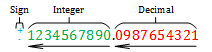
\includegraphics[scale=1.0]{./algorithm/real/pic/design/data_format_v2.png}
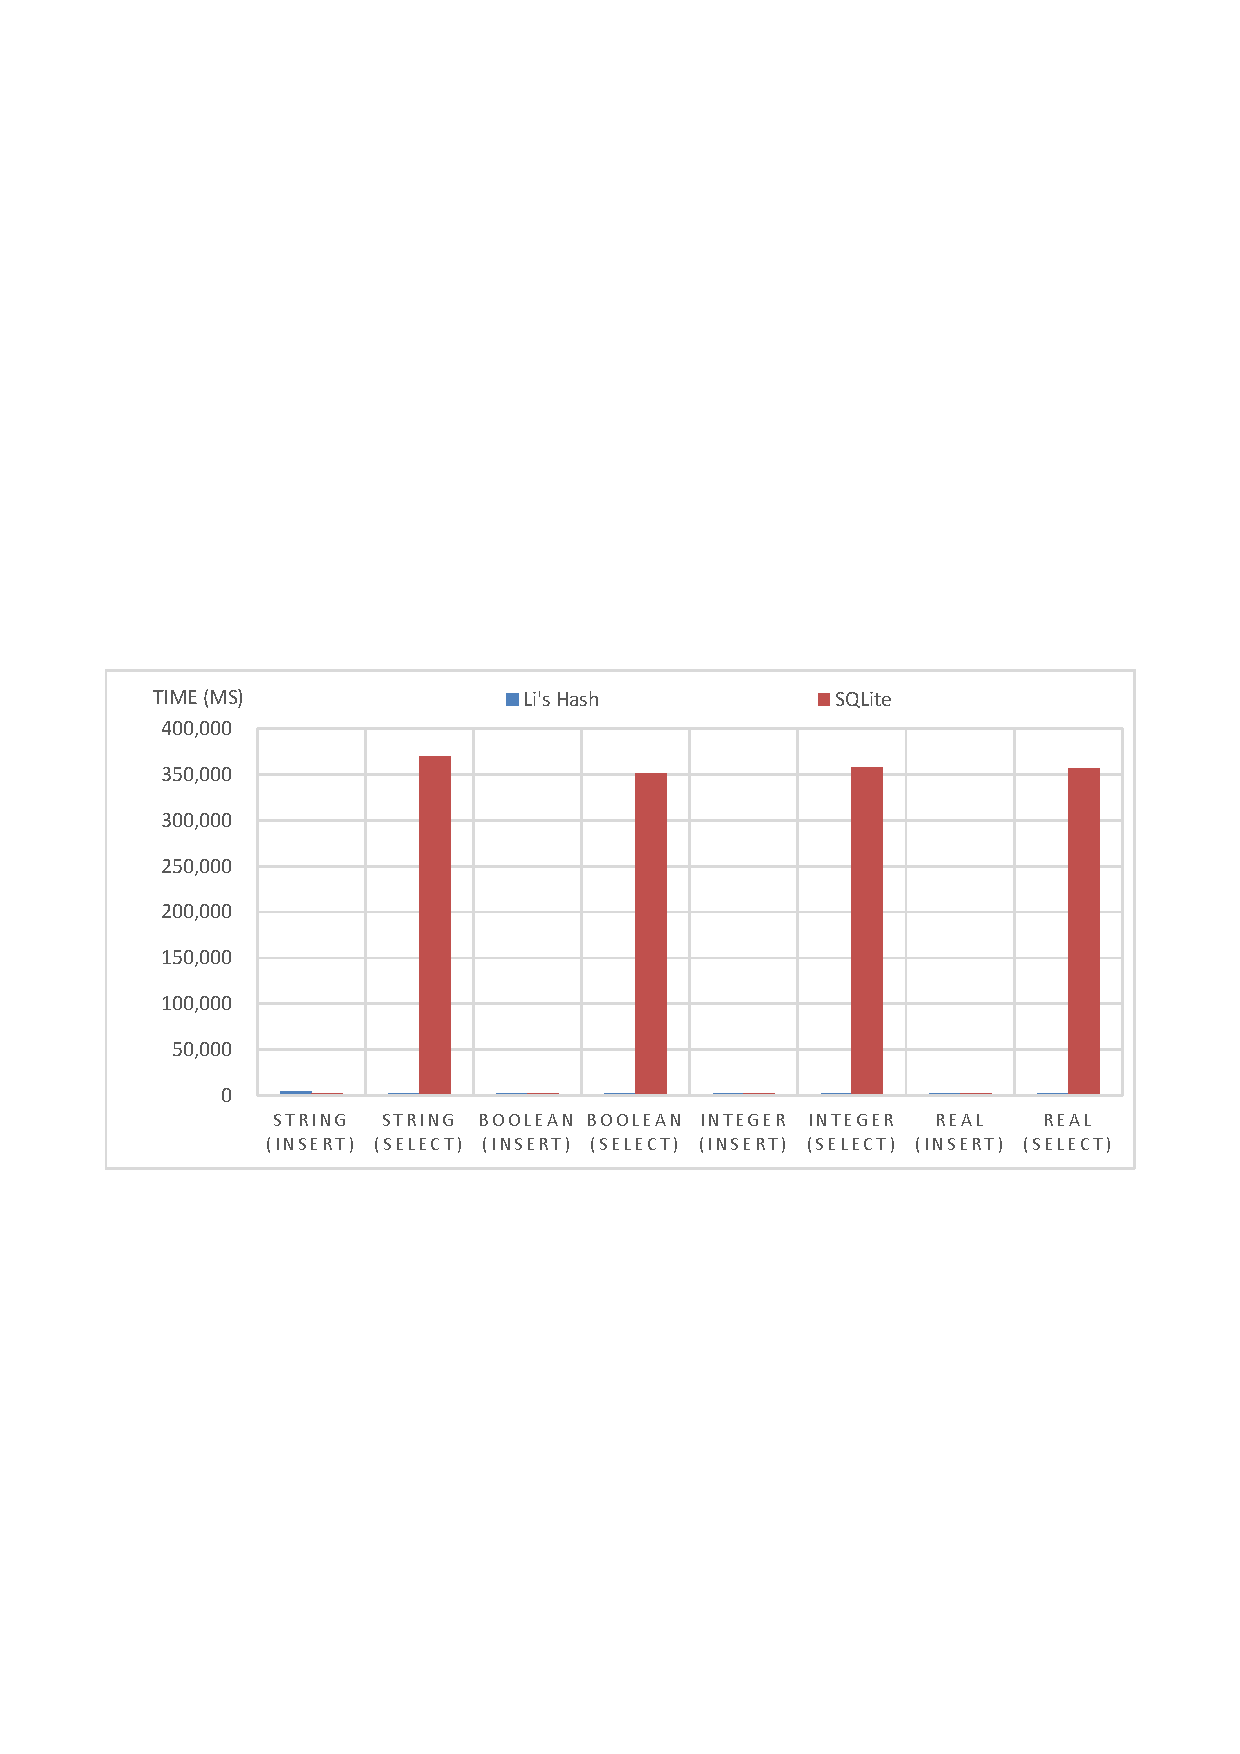
\includegraphics[width=0.8\textwidth]{./performance/result/database-layer/image/100only/full2.pdf}
\caption{Performance on database layer}
\label{fig:performance:result:database-layer}
\end{figure*}



\clearpage

% ----------------------------------------------------------

% Index layer section
\item \textbf{Index layer}

Fellow the test in \textit{Database layer}, but this time we include the index part, remove(), update() for Li's Hash. Also test DELETE, UPDATE with enable the index in relational database which using the code of table \ref{table:performance:index-layer:code-example}.\\

% Index layer test table 

% Index layer test
\begin{table*}[width=\textwidth]
\centering
\caption{Example code that to test STRING type in \textit{Index layer}}
\label{table:performance:index-layer:code-example}
\begin{tabular}{|c|c|c|}

\hline
\multicolumn{1}{|c|}{} &
\multicolumn{1}{c|}{\textbf{Li's Hash}} &
\multicolumn{1}{c|}{\textbf{Relational database}} \\

\hline
\multicolumn{1}{|c|}{Create table} &
\multicolumn{1}{l|}
{\tabincell{l}{
create\_table('table', 'value', STRING\_TYPE)
}} &
\multicolumn{1}{l|}
{\tabincell{l}{
CREATE TABLE table(id INT, value TEXT) ; \\
CREATE INDEX idx\_value ON table (value) ;
}} \\

\hline
\multicolumn{1}{|c|}{Insert} &
\multicolumn{1}{l|}
{\tabincell{l}{
insert('table', 'value-\textit{i}')
}} &
\multicolumn{1}{l|}
{\tabincell{l}{
INSERT INTO table('value') VALUES ('value-\textit{i}') ;
}} \\

\hline
\multicolumn{1}{|c|}{Select} &
\multicolumn{1}{l|}
{\tabincell{l}{
select('table', 'value', 'value-\textit{i}')
}} &
\multicolumn{1}{l|}
{\tabincell{l}{
SELECT value FROM table \\
WHERE value = 'value-\textit{i}' ;
}} \\

\hline
\multicolumn{1}{|c|}{Update} &
\multicolumn{1}{l|}
{\tabincell{l}{
update('table', 'value', 'value-\textit{i}', 'value-\textit{i}-')
}} &
\multicolumn{1}{l|}
{\tabincell{l}{
UPDATE table SET 'value' = 'value-\textit{i}-' \\
WHERE value = 'value-\textit{i}' ;
}} \\

\hline
\multicolumn{1}{|c|}{Remove} &
\multicolumn{1}{l|}
{\tabincell{l}{
remove('table', 'value', 'value-\textit{i}-')
}} &
\multicolumn{1}{l|}
{\tabincell{l}{
DELETE FROM table WHERE value = 'value-\textit{i}' ;
}} \\

\hline
\end{tabular}
\end{table*}



% Index layer result 

\begin{figure*}
        \centering

        \begin{subfigure}[b]{0.4\textwidth}
                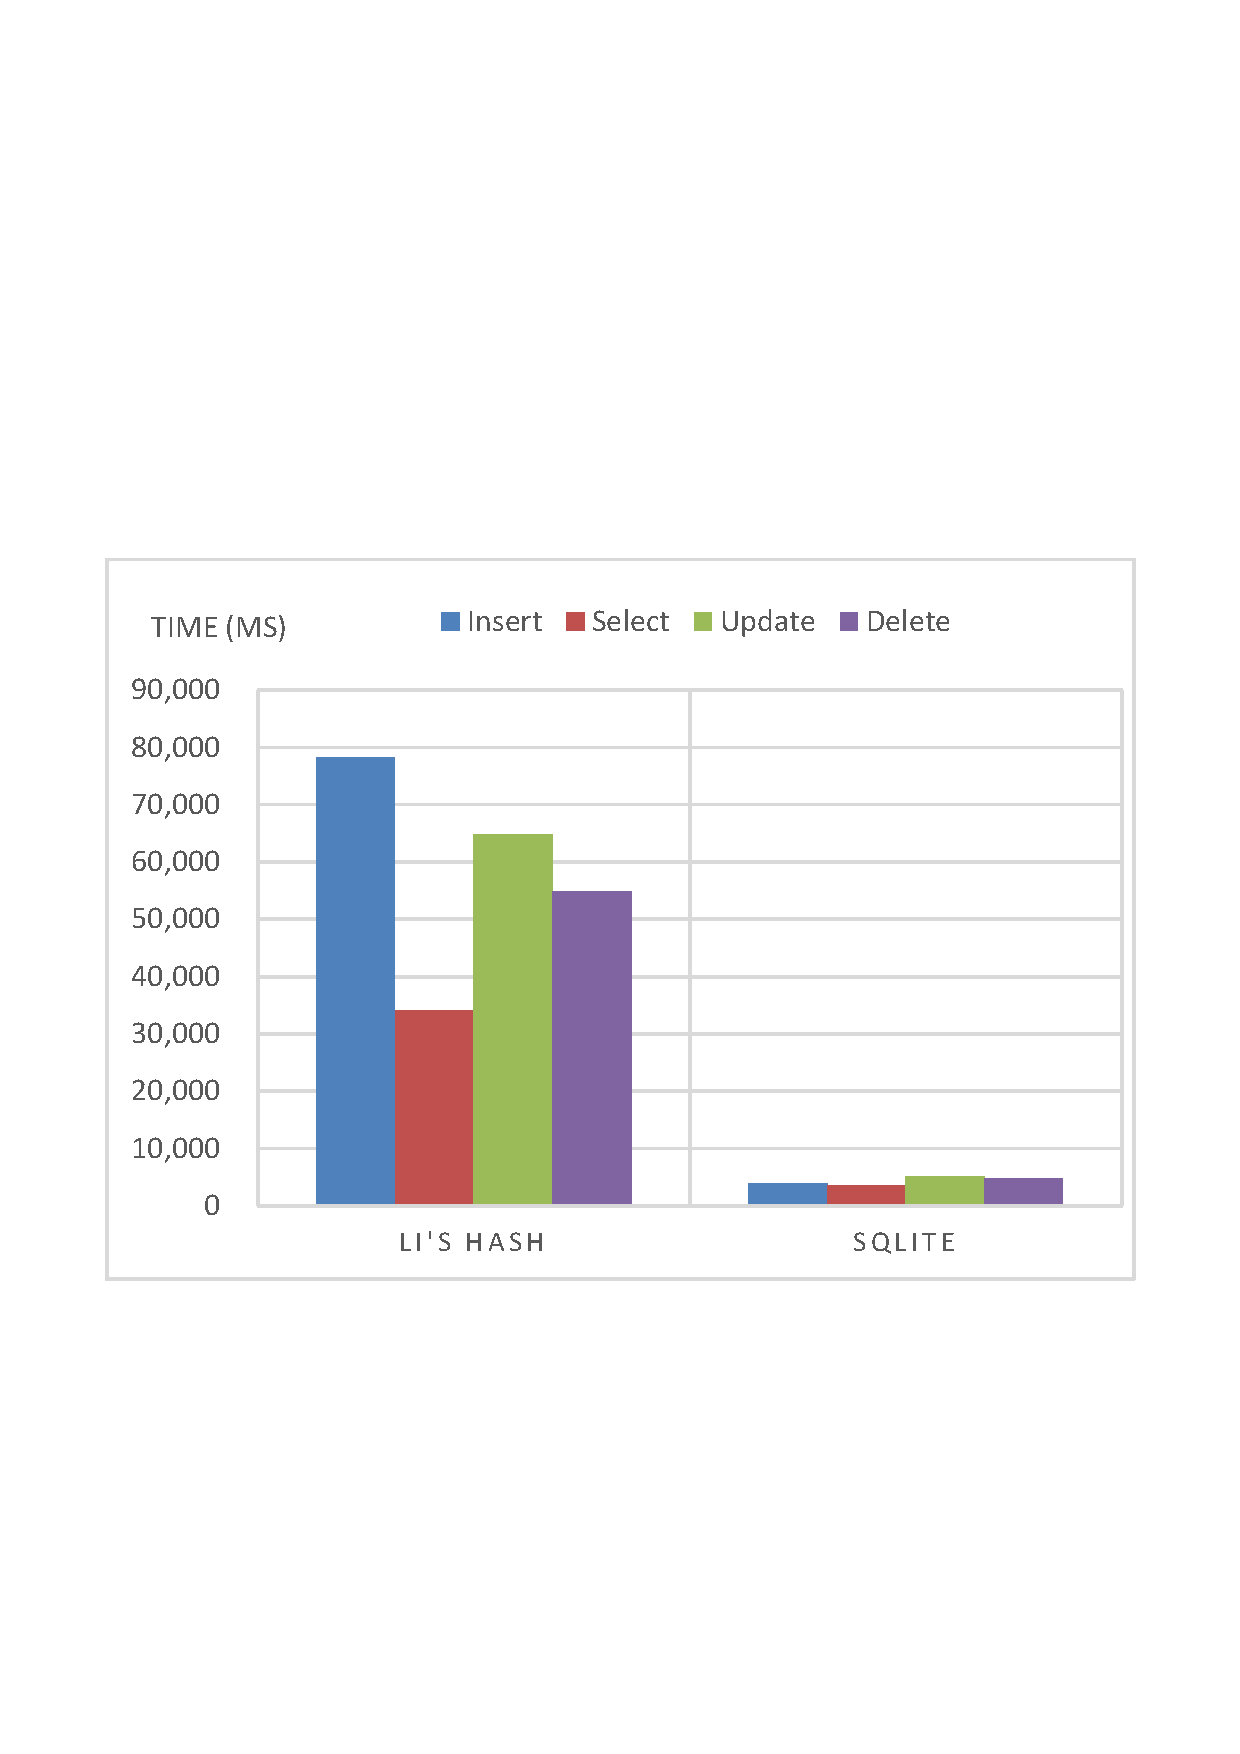
\includegraphics[width=\textwidth]{./performance/result/index-layer/image/100only/string1.pdf}
                \caption{STRING type}
                \label{fig:performance:result:index-layer:insert:boolean}
        \end{subfigure}%
        ~ %add desired spacing between images, e. g. ~, \quad, \qquad etc.
          %(or a blank line to force the subfigure onto a new line)
        \begin{subfigure}[b]{0.4\textwidth}
                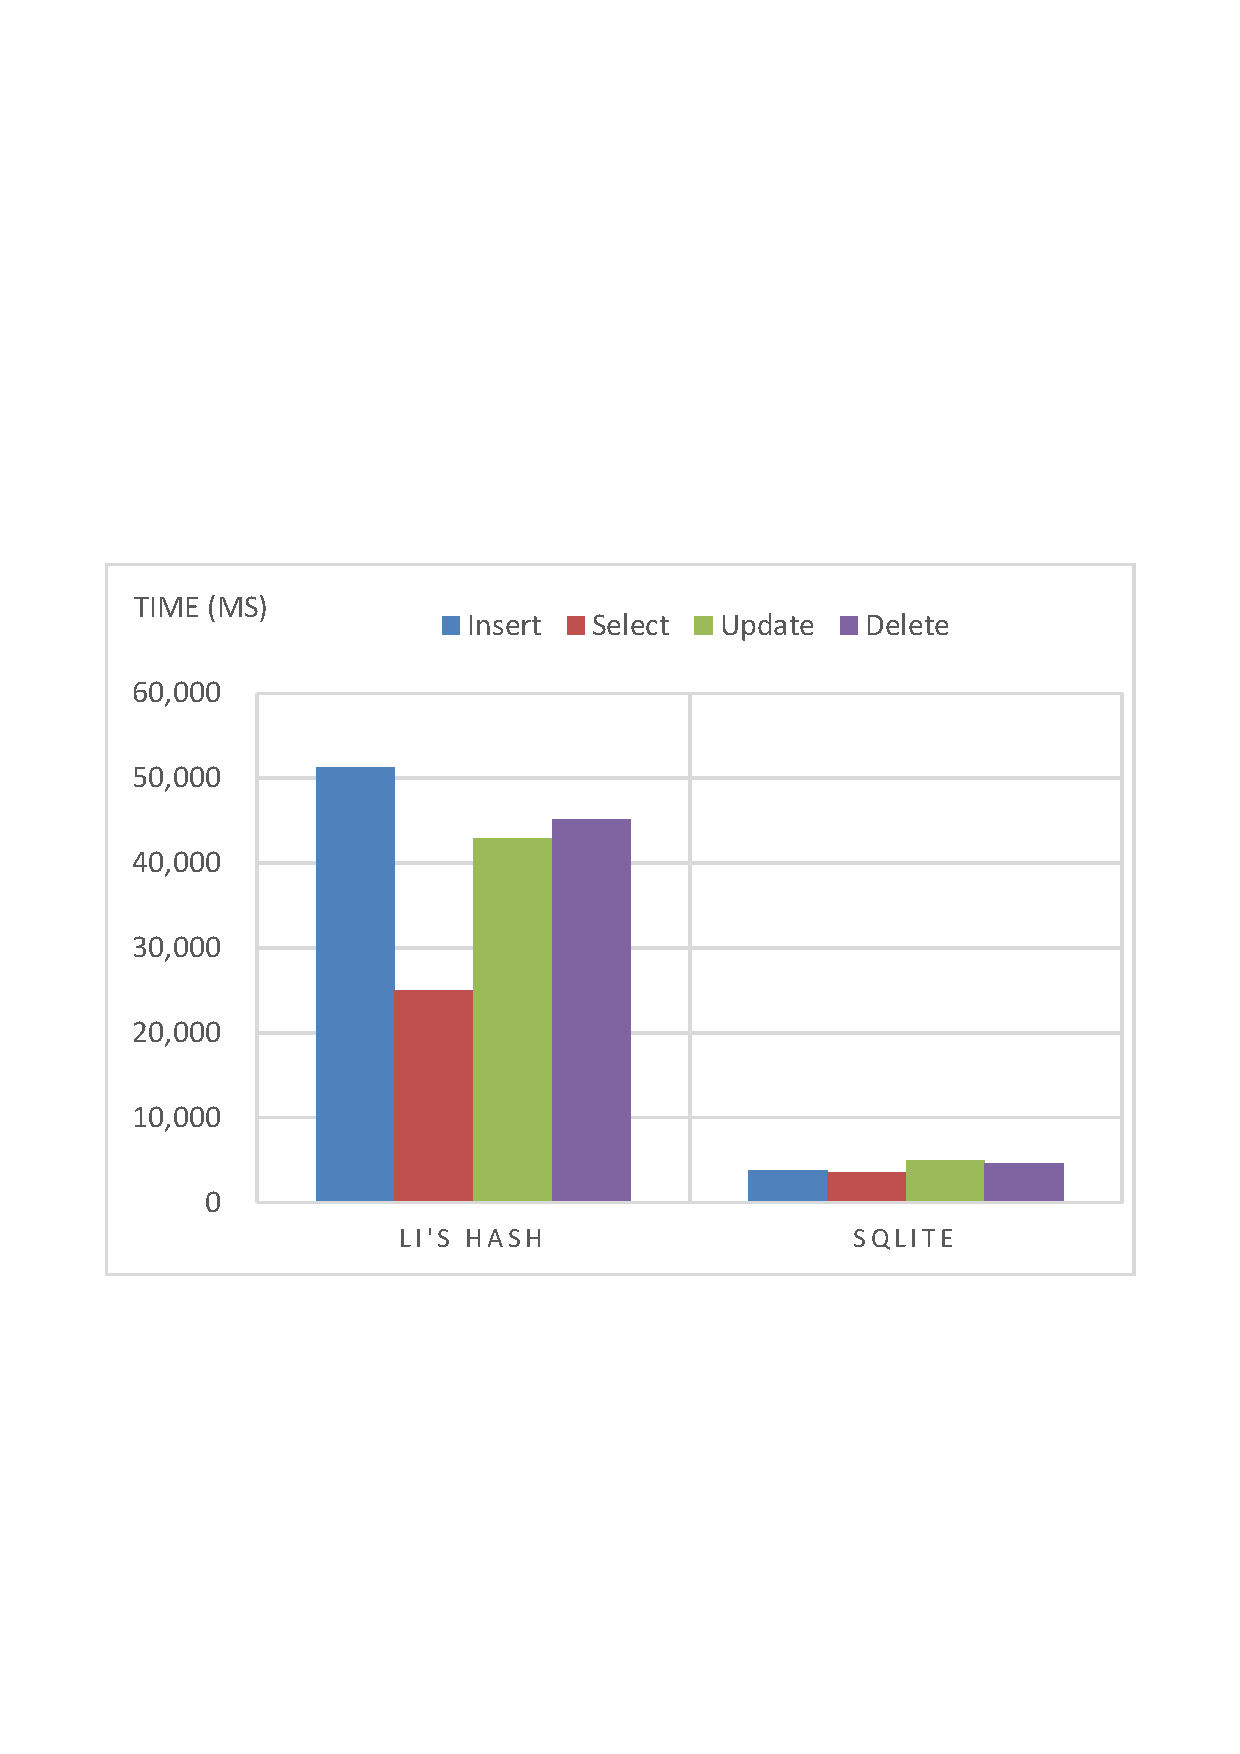
\includegraphics[width=\textwidth]{./performance/result/index-layer/image/100only/boolean1.pdf}
                \caption{BOOLEAN type}
                \label{fig:performance:result:index-layer:insert:int}
        \end{subfigure}

        \begin{subfigure}[b]{0.4\textwidth}
                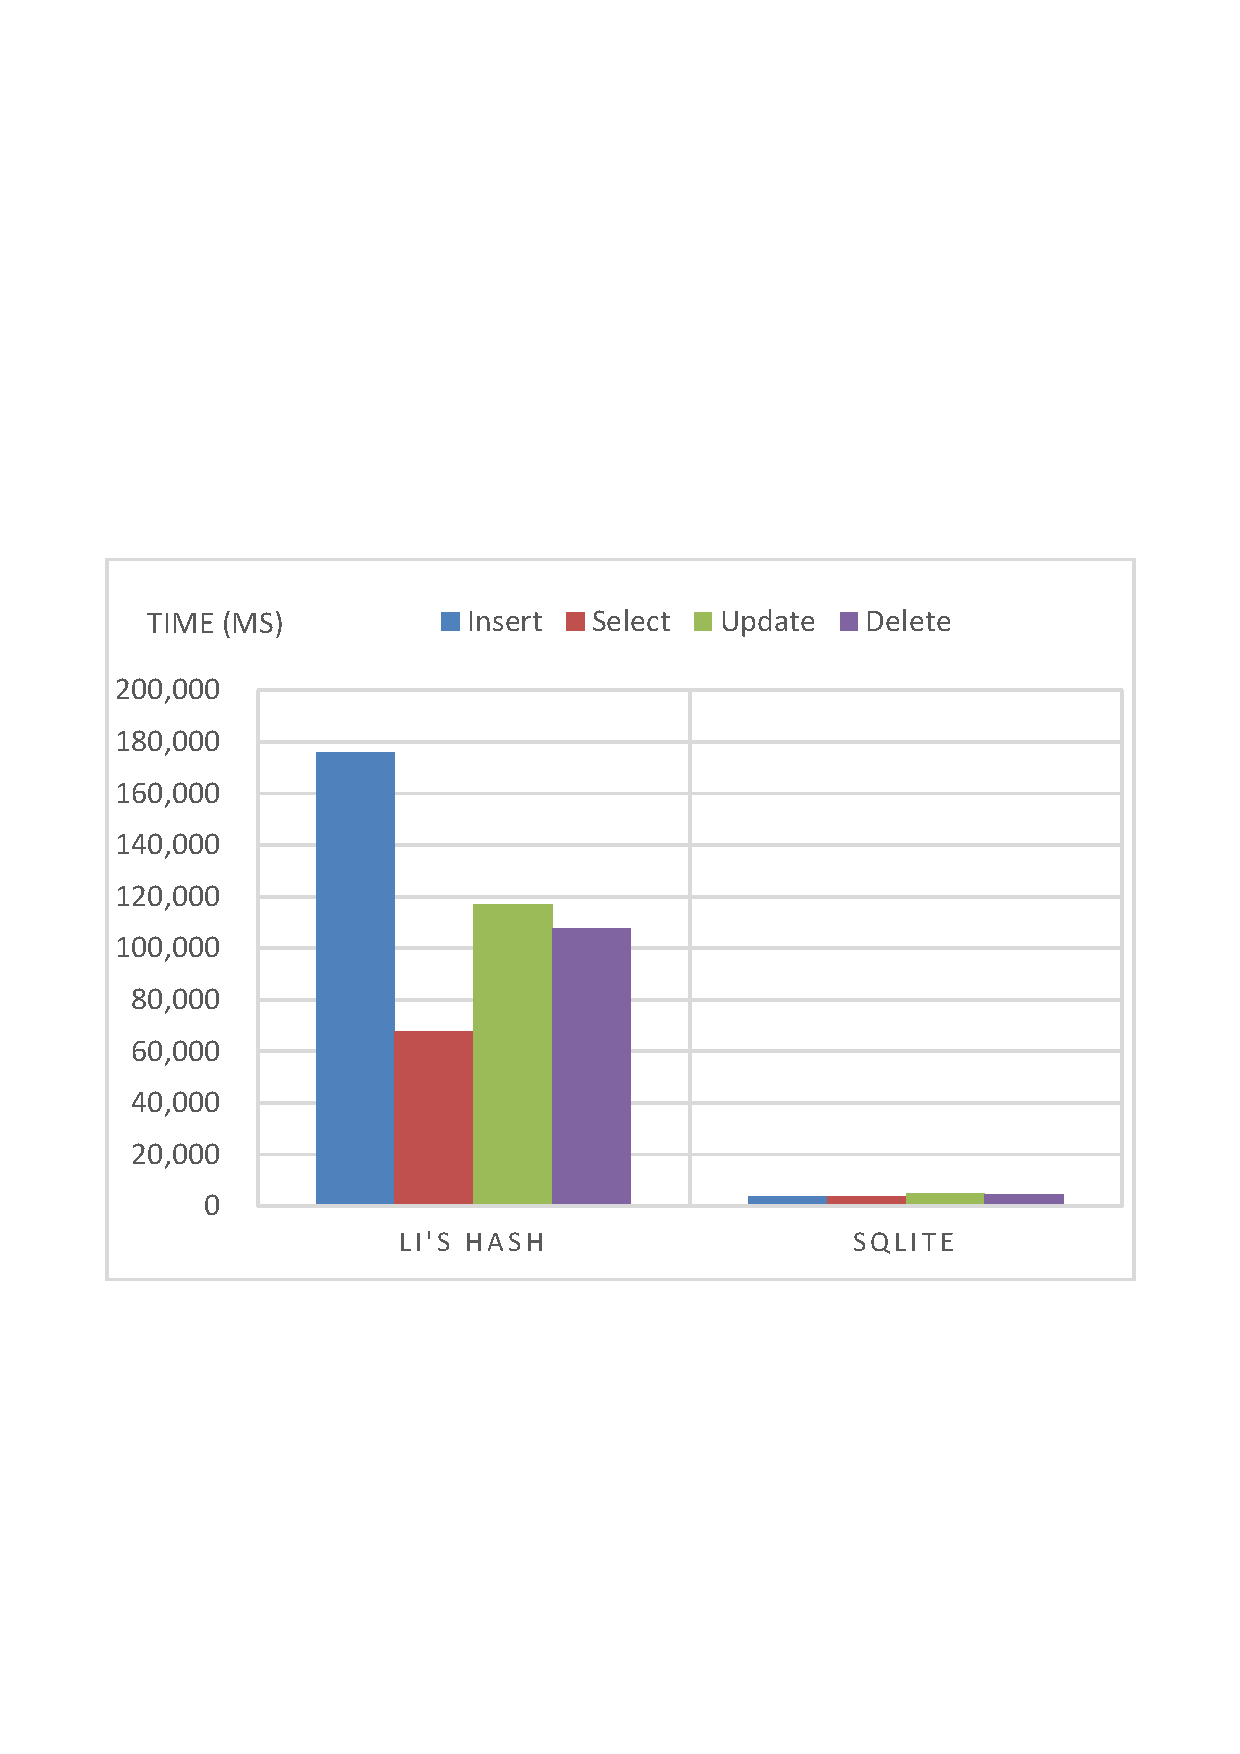
\includegraphics[width=\textwidth]{./performance/result/index-layer/image/100only/integer1.pdf}
                \caption{INTEGER type}
                \label{fig:performance:result:index-layer:insert:real}
        \end{subfigure}
        ~ %add desired spacing between images, e. g. ~, \quad, \qquad etc.
          %(or a blank line to force the subfigure onto a new line)
        \begin{subfigure}[b]{0.4\textwidth}
                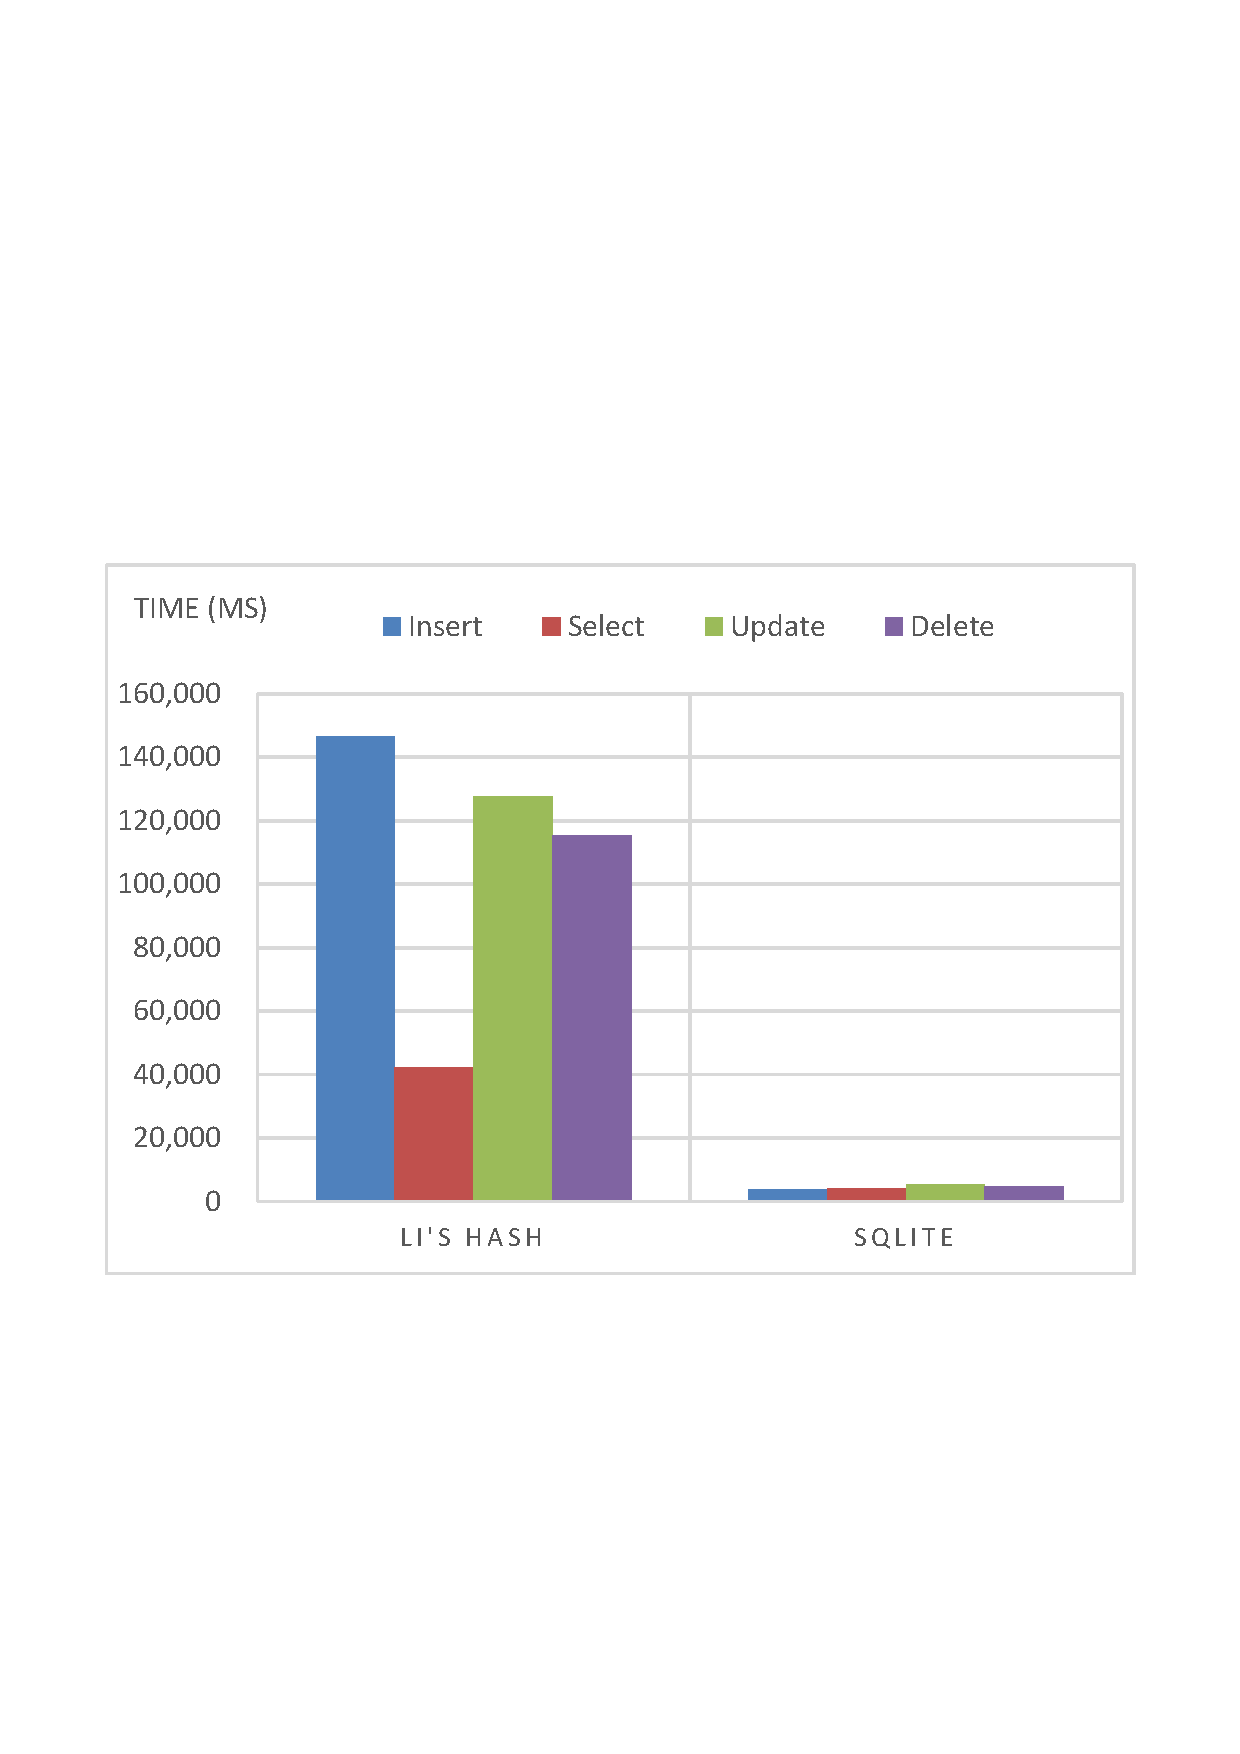
\includegraphics[width=\textwidth]{./performance/result/index-layer/image/100only/real1.pdf}
                \caption{REAL type}
                \label{fig:performance:result:index-layer:insert:string}
        \end{subfigure}

        \caption{Performance on index layer}
        \label{fig:performance:result:index-layer}
\end{figure*}



\clearpage

% ----------------------------------------------------------

% Joining section
\item \textbf{Joining operation}

Joining always is one of the bottleneck of the relational database, but it is just a intersection operation for Li's Hash. So in this test, we let them to do the a mutli-table joining.\\

\begin{figure}[h]
\centering
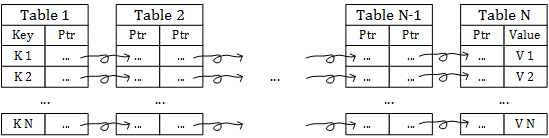
\includegraphics[scale=0.8]{./performance/pic/multi-table_v1.png}
\caption{A example of mutli-table joining.}
\label{fig:performance:multi-table}
\end{figure}

The mutli-table is look like figure \ref{fig:performance:multi-table}, this example is a very sample joining in Human thought, but it still can be a over-hand of the relational database. This example is just search the value by joining many table in the middle, the starting point is the column "Key" in Table 1 and finish is the "Value" column in the Table N, between them is a ton of the pointer which is use for pointing to the next pointer in the next table, so that when search the value which will need to joining these tables and pointer to get the correct value.\\

So this should need to use complex SQL and need times to do that, which will get our a result that the Li's Hash can do the  joining operation and a better time.\\

\clearpage

% ----------------------------------------------------------

\end{enumerate}

% Result section
\subsection{Result}

Figure \ref{fig:performance:result:database-layer} and \ref{fig:performance:result:index-layer} are shows that it is faster after enabled the indexing in SQLite, also Li's Hash become slower because the indexing rather directly using the \textit{put()} or \textit{get()} that because it need to build the index table.\\

In this testing, the main point is not to test how good as the Li's Hash compare to a well-known embedded relational database, but to test it is workable or not, so our will focus on the improvement and the application extension (such as graph database, base on the same table design) to provide different angle and usage.\\

\clearpage

% ------------------------------------------------
% End of page
% ------------------------------------------------


% Conclusion chapter
%% ------------------------------------------------
\StartChapter{Conclusion}{chapter:conclusion}
% ------------------------------------------------

Write your conclusion here.

% ------------------------------------------------
\EndChapter
% ------------------------------------------------


% Future work chapter
%% ------------------------------------------------
% Page start
% ------------------------------------------------
\chapter{Future work}
\label{chapter:future-work}

\baselineskip=26pt
\thispagestyle{empty}
% ------------------------------------------------

The next step of Li's Hash is focus on the improvement and the application extension (such as graph database, base on the same table design) to provide different angle and usage.\\

Later on, by adding the SQL parser into the library for handle SQL as the input, which should let the people more comfortable to use it like the normally SQL database. Also provide some more feature for the library is needed, such as multi-table joining operation in SQL, graph database (like Neo4j\cite{web:neo4j:home-page}, by using different back-end database rather than a fixed storage engine), decision tree, similarity (like Lucene \cite{web:wiki:lucene}), etc. These feature are very basic and common that should become very useful in many field, such as information retrieval and data mining.\\

%\clearpage

% ------------------------------------------------
% End of page
% ------------------------------------------------


% ------------------------------------------------

% 參考文獻 References
%
% ----------------------------------------------------------------------------
%                                 References
%                                   參考文獻
% ----------------------------------------------------------------------------

% Page start
\newpage
\phantomsection

% Add to "Table of Contents"
%\addcontentsline{toc}{chapter}{References}

% Change the title of bibliography
%\renewcommand\bibname{\centerline{\Large References}}

% ------------------------------------------------

\bibliographystyle{abbrv}
\bibliography{./example/references/paper,./example/references/msic}

% ------------------------------------------------
% End of page
% ------------------------------------------------


% ------------------------------------------------

% 附錄 Appendix
%% ------------------------------------------------
\StartAppendix
% ------------------------------------------------

% ------------------------------------------------
% Page start
\newpage
\phantomsection
% ------------------------------------------------

\chapter{可使用這模版的系所}
\label{appendix:acceptable-dept}

這邊列出一些\textbf{應該可使用}或\textbf{不可使用}這模版的系所名字, 這表可能會有不正確, 所以還是先問系辦確定會比較好.\\

因為這名單都是靠網路上能找多少而得出的結果, 而如果沒有分類的話, 很高機會是使用圖書館的要求. \\

而如果這表名單中沒有顯示你的系所, 但你已經\textbf{知道}是否能使用, 請告知以供更新.

\clearpage

\section{應該可使用}

    可使用的原因幾乎都是系所自己沒有特殊要求, 所以直接使用圖書館的要求, 而本模版就是跟隨圖書館所定下的要求來設計.

    \begin{table*}[pht]
    \centering
    \caption{應該可使用的系所}
    \label{table:acceptable-dept:acceptable}
    \begin{tabular}{|c|c|}

    \hline
    \multicolumn{1}{|c|}{資訊工程學系} &
    \multicolumn{1}{c|}{Department of Computer Science and Information Engineering} \\

    \hline
    \end{tabular}
    \end{table*}

\section{應該不可使用}

    不可使用的原因是系所自己已經有提供一份樣版出來, 而那份樣版的要求有沒有跟本模版一樣設計, 這個就不作詳細分析. 故如果已經有樣版, 那我就會把它們分類成\textit{無法使用這本模版}比較好, 但如果分類錯誤, 請告知.

    \begin{table*}[pht]
    \centering
    \caption{應該不可使用的系所}
    \label{table:acceptable-dept:unacceptable}
        \begin{tabular}{|c|c|c|}

        \hline
        \multicolumn{1}{|c|}{生物科技研究所} &
        \multicolumn{1}{c|}{Institute of Biotechnology} &
        \multicolumn{1}{c|}{\href{www.biotech.ncku.edu.tw/files/archive/331_4b79187a.doc}{樣版URL}} \\

        \hline
        \multicolumn{1}{|c|}{體育健康與休閒研究所} &
        \multicolumn{1}{c|}{
            \tabincell{l}{
            Institute of Physical Education,\\
            Health and Leisure Studies
            }
        } &
        \multicolumn{1}{c|}{\href{www.ncku.edu.tw/~deprb/docs/Thesis\%20Regulation\%20.doc}{樣版URL}} \\

        \hline
        \end{tabular}
    \end{table*}

% ------------------------------------------------
% End of page
% ------------------------------------------------

%% ------------------------------------------------
\StartChapter{繳交流程說明}
% ------------------------------------------------

這部份資料來源是使用'電子學位論文服務'提供的'電子學位論文服務流程說明圖'\RefBib{web:lib:submit-flow}和'繳交論文全文電子檔案說明'\RefBib{web:lib:submit-file}.\\

\setboolean{@twoside}{false}
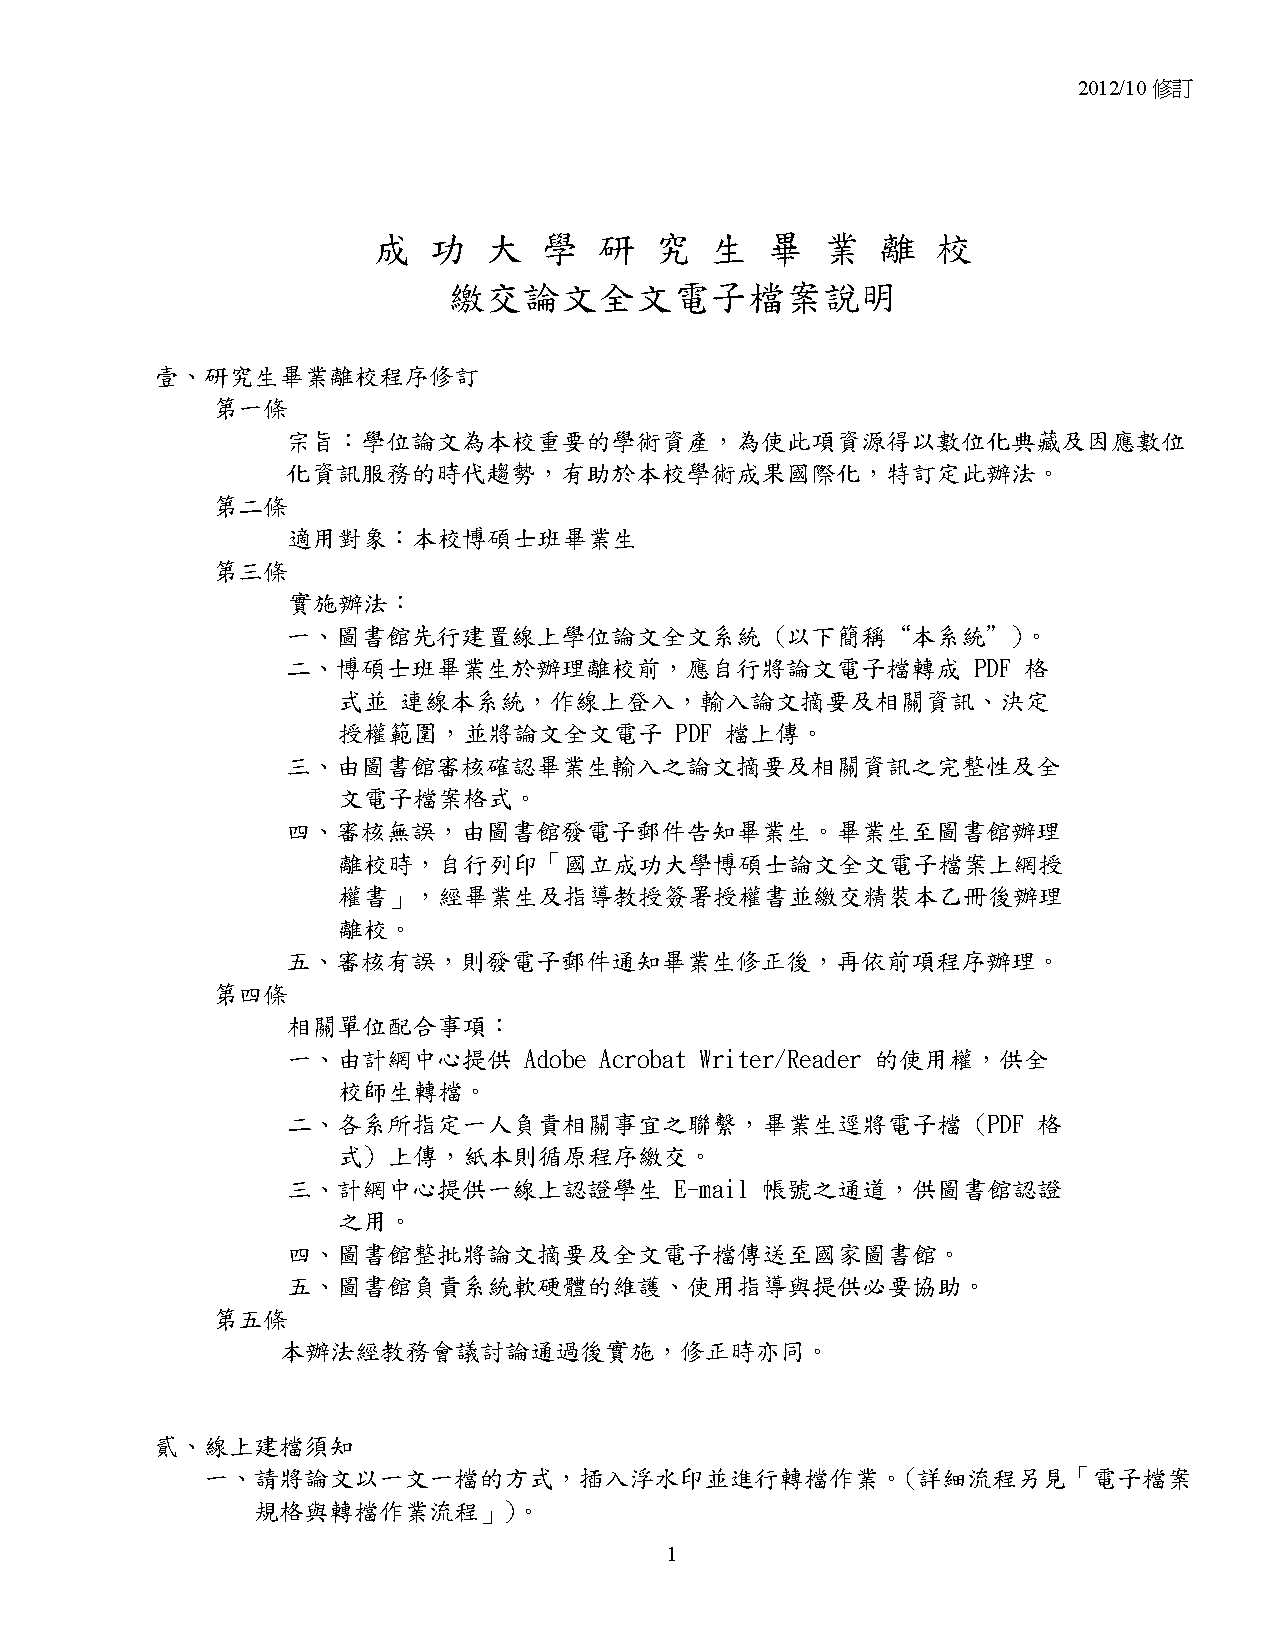
\includepdf[pages=-]{./example/appendix/pdf/2012050004-a.pdf}
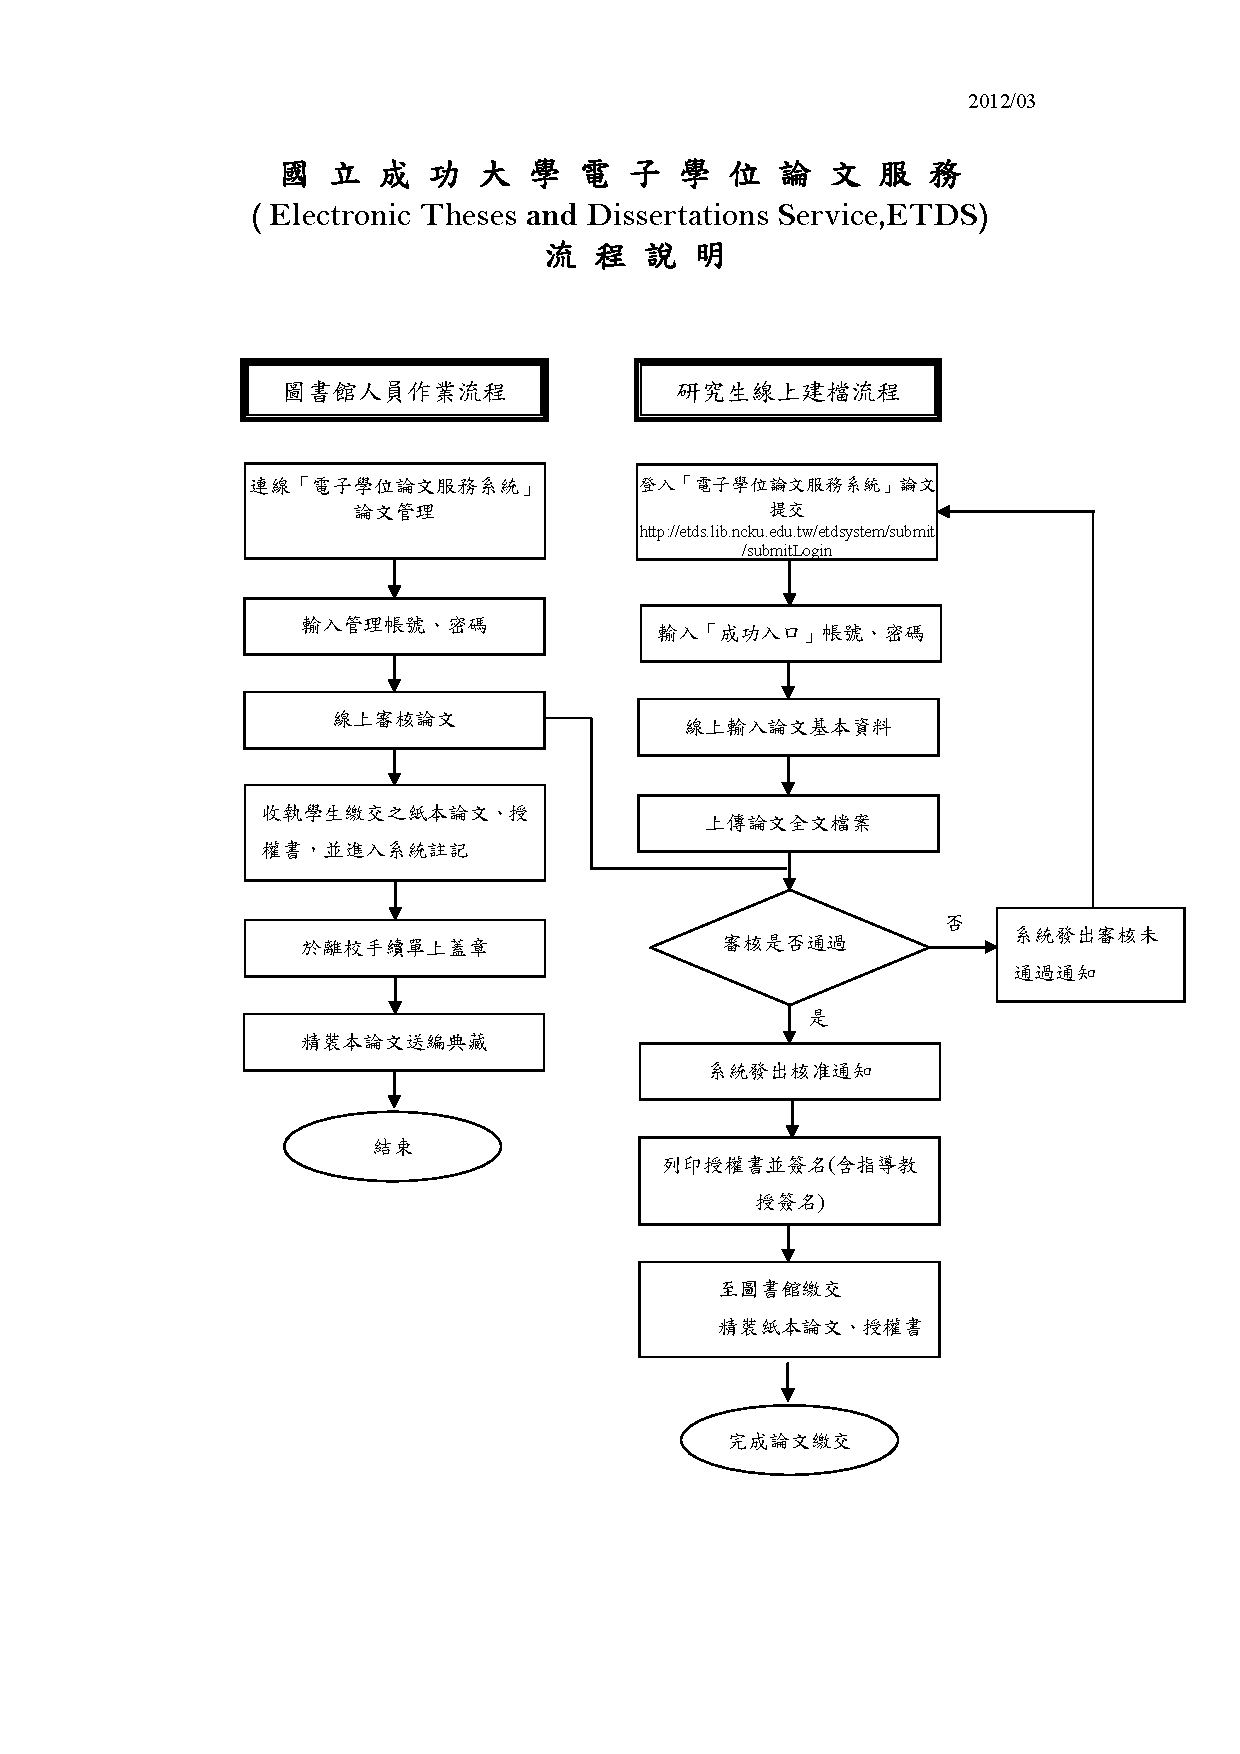
\includepdf[pages=-]{./example/appendix/pdf/2012050006-a.pdf}

% ------------------------------------------------
\EndChapter
% ------------------------------------------------

% ------------------------------------------------
% Page start
\newpage
\phantomsection
% ------------------------------------------------

\chapter{各系所博碩士撰寫論文須知}
\label{appendix:thesis-spec}

\section{介紹}
這部份資料來源是使用'電機工程系辦網頁'中的'論文撰寫須知.pdf'(\url{http://office.ee.ncku.edu.tw/uploads/%E8%AB%96%E6%96%87%E6%92%B0%E5%AF%AB%E9%A0%88%E7%9F%A5.pdf}).\\

但由於原檔案沒法顯示, 故需要另重新儲存成一個新的出來. 使用學校的Adobe Acrobat XI試驗, 發現要使用'儲存為其他->可存檔PDF (PDF/A)'才能顯示出來.\\

\begin{figure}[h]
\centering
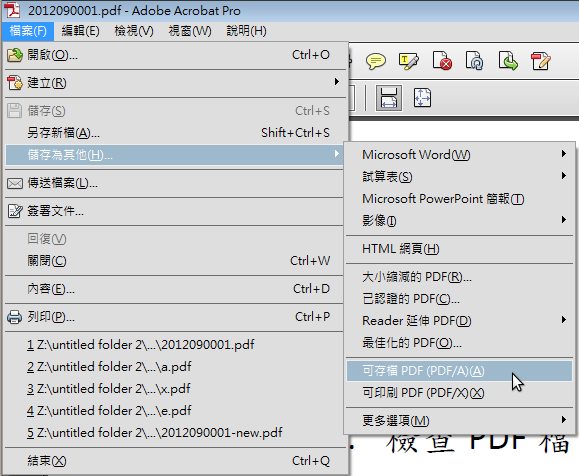
\includegraphics[scale=0.3]{./example/appendix/pic/save_pdf.png}
\caption{在Adobe Acrobat另存新版本}
\label{fig:appendix:save_pdf}
\end{figure}

檔案位置:\\
新: 'example/appendix/pdf/thesis-spec.pdf'\\
原: 'example/appendix/pdf/論文撰寫須知.pdf'\\

\setboolean{@twoside}{false}
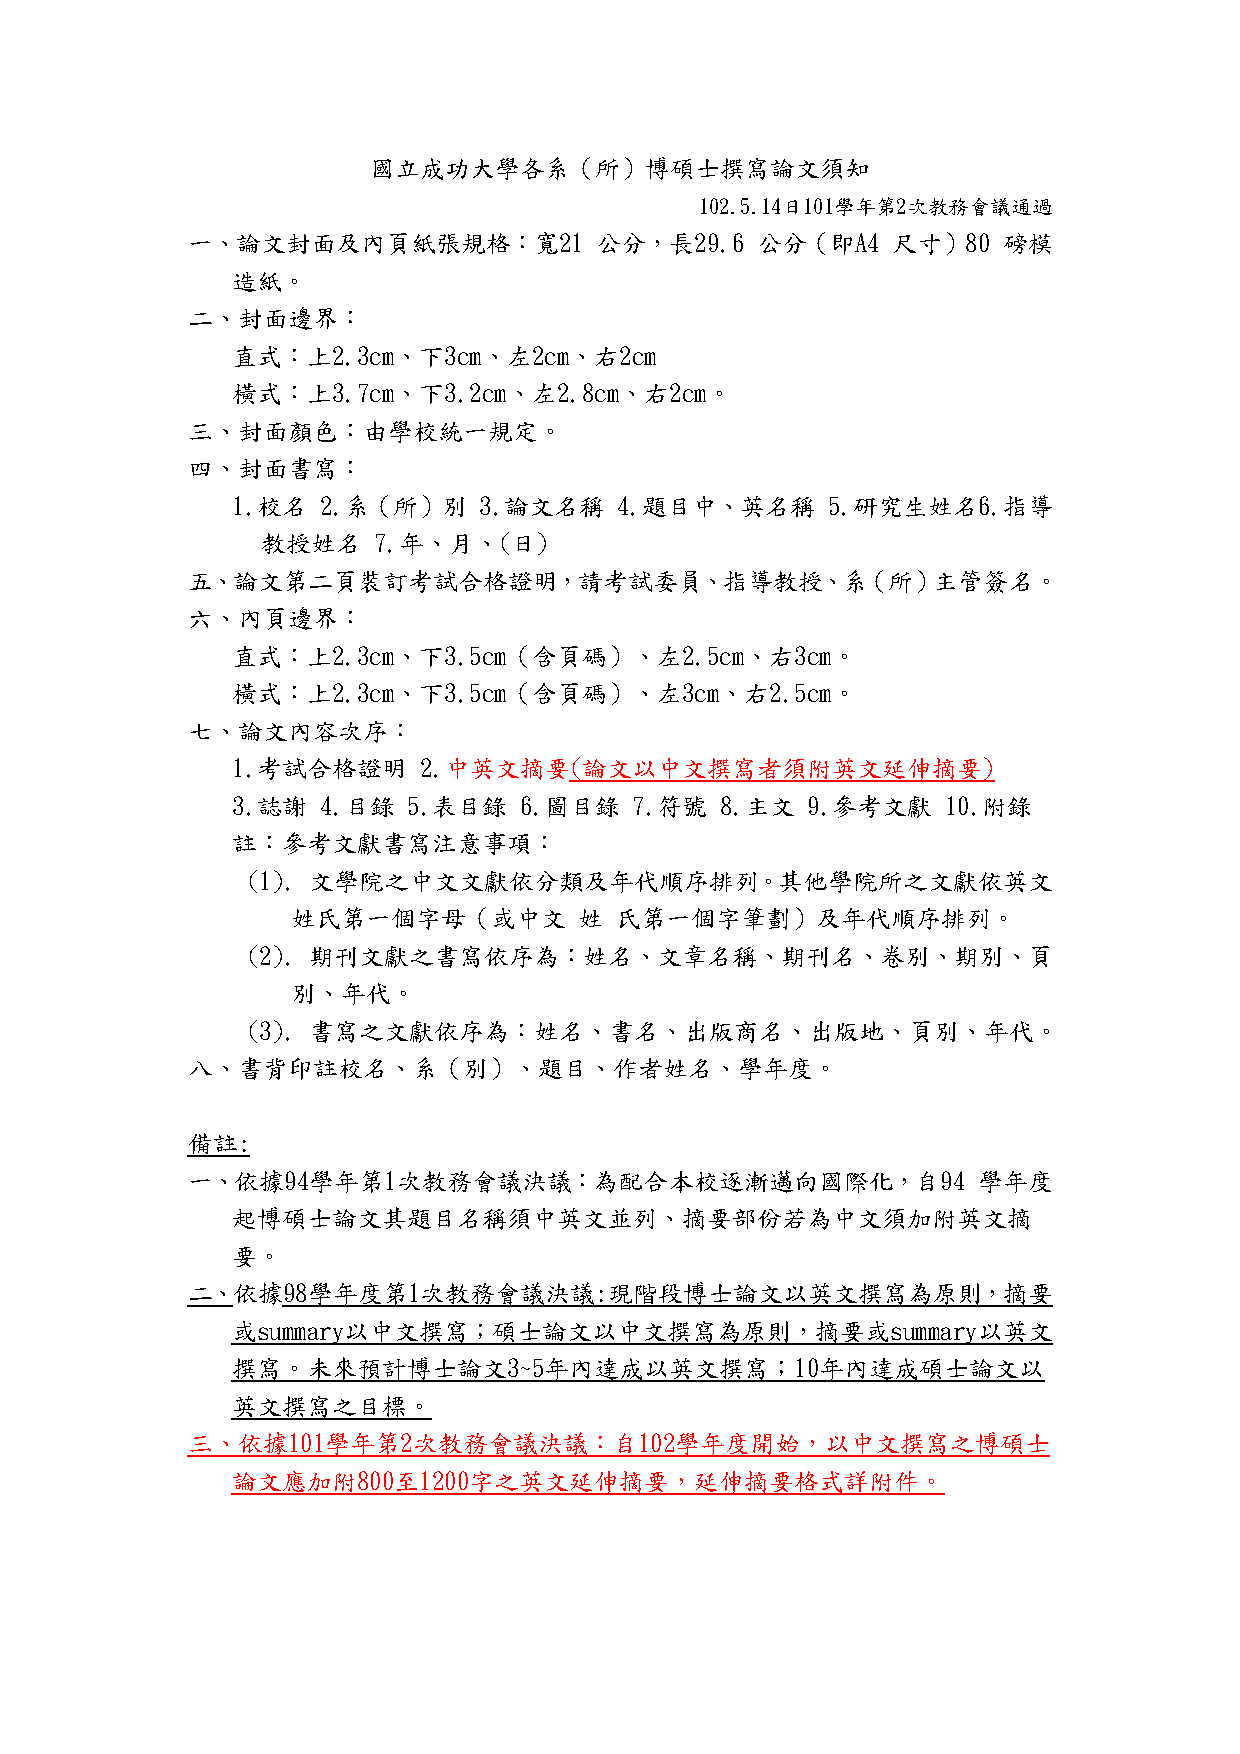
\includepdf[pages=-]{./example/appendix/pdf/thesis-spec.pdf}

% ------------------------------------------------
% End of page
% ------------------------------------------------

%% ------------------------------------------------
\StartChapter{電子論文上傳前檢查事項}{appendix:e-paper_upload}
% ------------------------------------------------

\section{介紹}
這部份資料來源是使用'成功大學電子學位論文服務'中的'電子論文上傳前檢查事項'的'2012090001.pdf'.\\

同樣原檔案沒法顯示, 故需要進行另儲存.\\

檔案位置:\\
新: 'example/appendix/pdf/2012090001-a.pdf'\\
原: 'example/appendix/pdf/2012090001.pdf'\\

\setboolean{@twoside}{false}
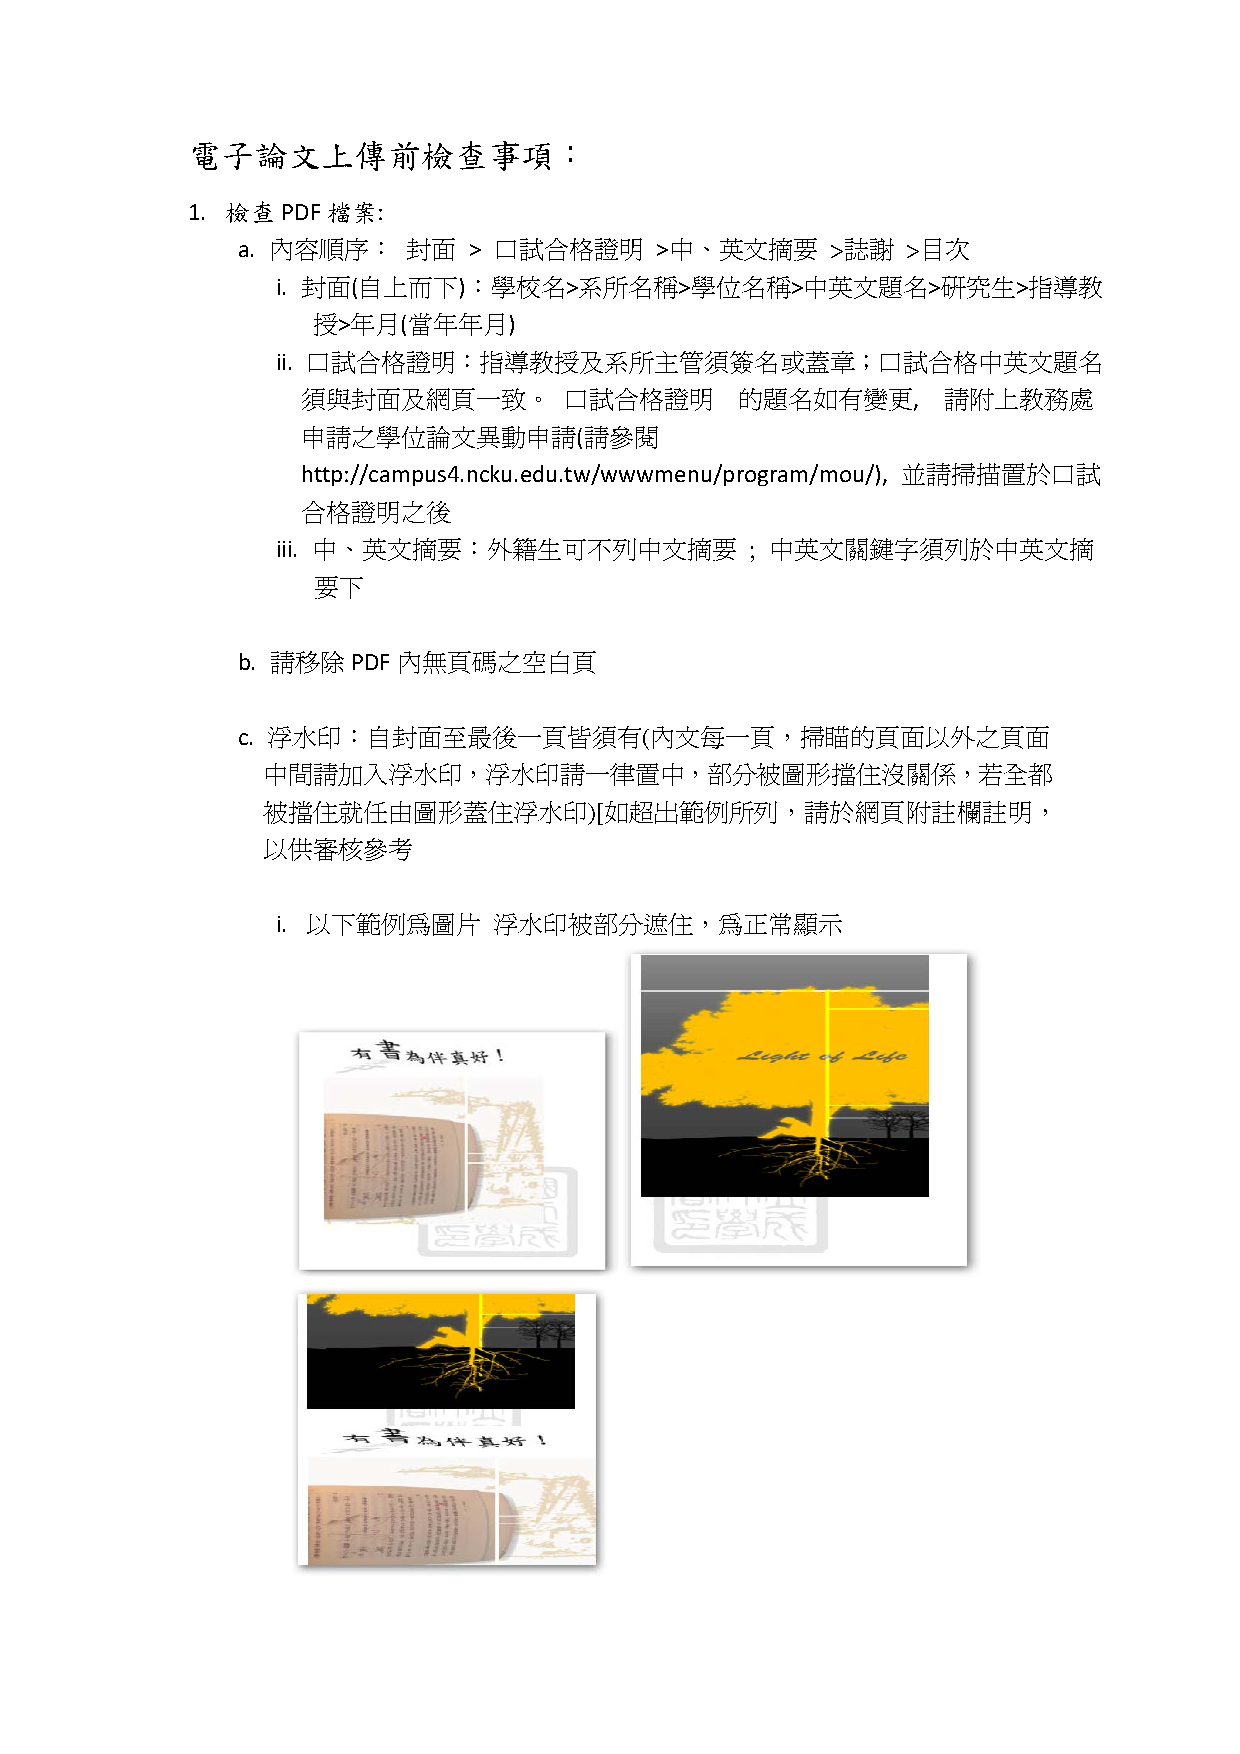
\includepdf[pages=-]{./example/appendix/pdf/2012090001-a.pdf}

% ------------------------------------------------
\EndChapter
% ------------------------------------------------

%% ------------------------------------------------
\StartChapter{學位論文上傳說明}{appendix:e-paper_upload_ppt}
% ------------------------------------------------

這部份資料來源是使用'電子學位論文服務'提供的 '2015論文提交說明簡報檔'\RefBib{web:lib:2015-submit-ppt} 修改而成的, 只抽出使用本模版後, 還要做什麼的行為.\\

\setboolean{@twoside}{false}
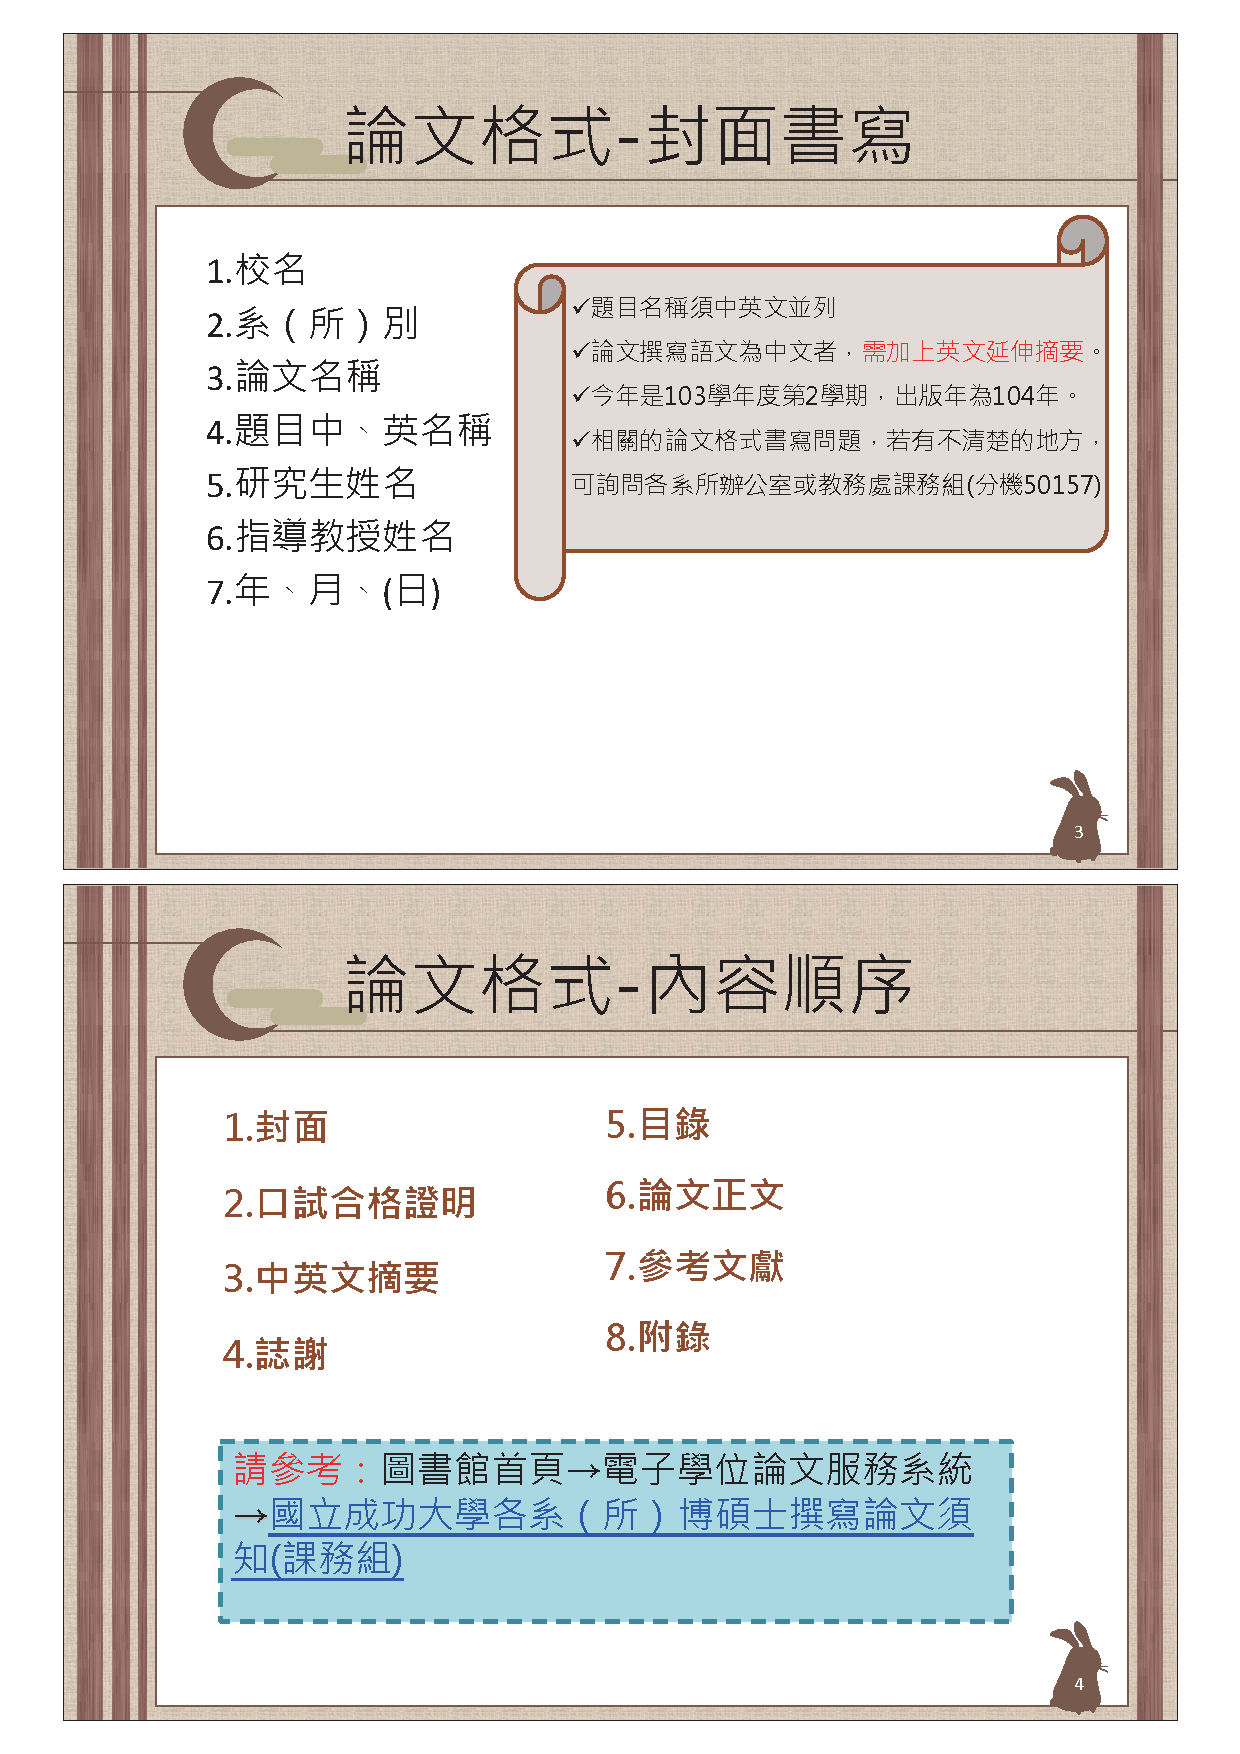
\includepdf[pages=-]{./example/appendix/pdf/2012050003-short-a}

% ------------------------------------------------
\EndChapter
% ------------------------------------------------


%% ------------------------------------------------
\StartChapter{口試注意事項}
% ------------------------------------------------

這部份資料來源是使用本系資訊工程研究所系辦所提供的資料, 雖然內容主要針對本系, 但某些內容都是適合非本系的同學們.

\setboolean{@twoside}{false}
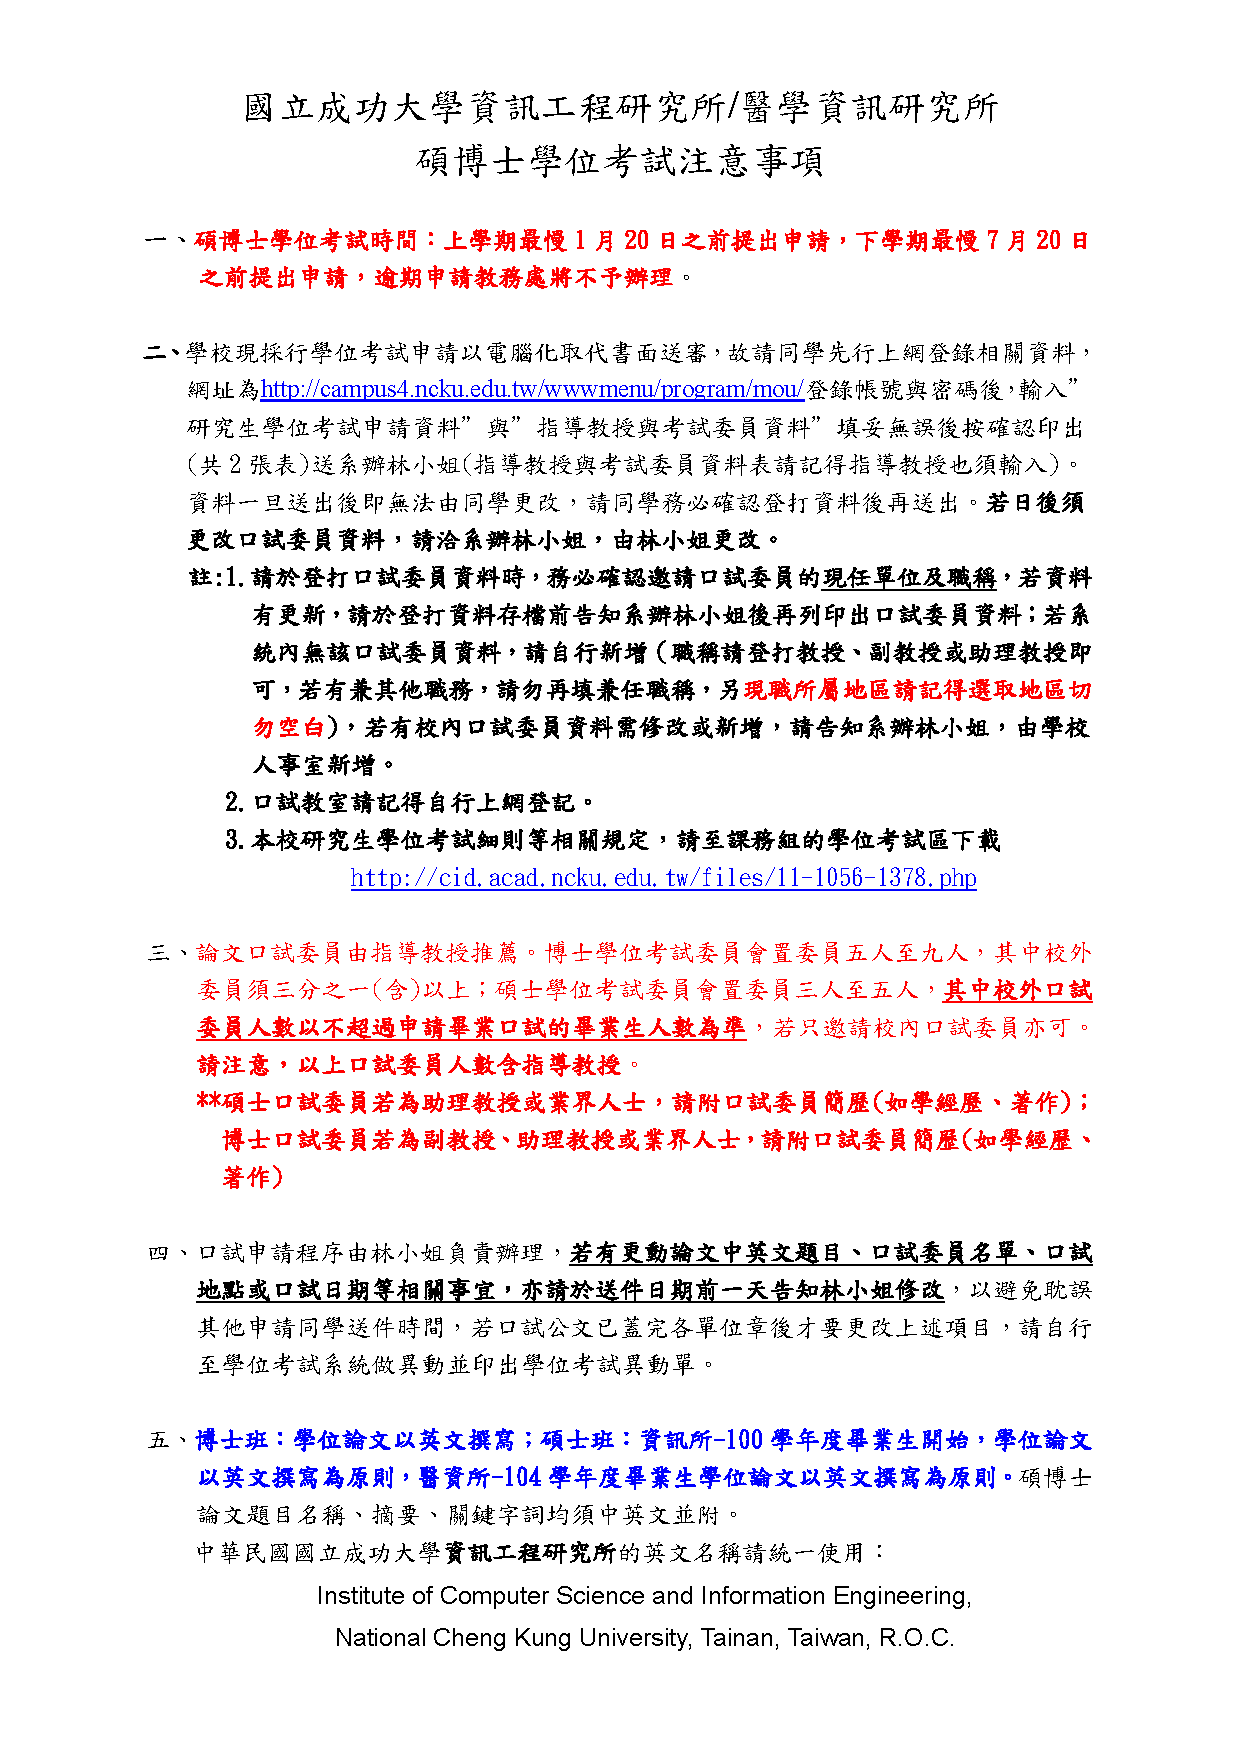
\includepdf[pages=-]{./example/appendix/pdf/oral-1040616-a.pdf}

% ------------------------------------------------
\EndChapter
% ------------------------------------------------

%% ------------------------------------------------
\StartChapter{常見問題Q\&A}{appendix:faq}
% ------------------------------------------------

\StartSection{介紹}
這部份資料來源是使用'電子學位論文服務'提供的'FAQ'\RefBib{web:lib:ETDS-QA}, 用來補充其他Appendix沒提到的一些情報.\\

\setboolean{@twoside}{false}
\includepdf[pages=-]{./example/appendix/pdf/2012050009-a.pdf}

% ------------------------------------------------
\EndChapter
% ------------------------------------------------

%% ------------------------------------------------
\StartChapter{LaTex Symbol寫法}{appendix:unicode-symbols}
% ------------------------------------------------

這部份資料來源是xeCJK的v3.3.4(2016/02/10)版本中提供的50頁有關所有Symbol的寫法, 極度值得同學們閱讀或在這邊找你所需的Symbols.\\

內容的說明方式為:\\
Symbol: 符號所顯示的樣子\\
USV: 以Unicode方式所代表的這個符號, 例如 `(' 的Unicode寫法為U+0028.\\
Description: 是這符號的名字.\\
Macro(s): 是LaTex使用這符號的寫法.\\

\textbf{P.S: }因為符號數量多, 沒法100\%保證全能使用.

\setboolean{@twoside}{false}
\includepdf[pages=-]{./example/appendix/pdf/xunicode-symbols.pdf}

% ------------------------------------------------
\EndChapter
% ------------------------------------------------


% ------------------------------------------------
\EndAppendix
% ------------------------------------------------


% ------------------------------------------------
